\documentclass{book}
\usepackage[utf8]{inputenc}
\usepackage[czech]{babel}
\usepackage{amsmath}
\usepackage{amssymb}
\usepackage{tikz}
\usepackage{siunitx}
\usepackage{environ}
\usetikzlibrary{math}
\usetikzlibrary{arrows.meta}

\newcommand{\eeql}[2]{
	\begin{equation}
	\begin{split}
	\label{#2}
	\input{out/eq_#1}
	\end{split}
	\end{equation}
}

\newcommand{\eeq}[1]{
\eeql{#1}{eq:#1}
}

\newcommand{\eeqn}[1]{
	\begin{equation}
	\begin{split}
	\input{out/eq_#1}
	\end{split}
	\end{equation}
}

\newcommand{\etab}[2]{
	\begin{table}[ht]
		\centering
		\input{out/tab_#1}
		\caption{#2}
		\label{tab:#1}
	\end{table}
}

\newcommand{\eimg}[2]{
	\begin{figure}[!h]
		\centering
		\begin{tikzpicture}
			\input{out/img_#1}
		\end{tikzpicture}
		\caption{#2}
		\label{img:#1}
	\end{figure}
}

\newcommand{\true}{\mathcal{P}}
\newcommand{\false}{\mathcal{N}}
\newcommand{\naturalnumbers}{\mathbb{N}}
\newcommand{\whole}{\mathbb{N}_0}
\newcommand{\integers}{\mathbb{Z}}
\newcommand{\rationals}{\mathbb{Q}}
\newcommand{\real}{\mathbb{R}}
\newcommand{\complex}{\mathbb{C}}
\newcommand{\imag}{\mathrm{i}}
\newcommand{\realpart}{\mathrm{Re}}
\newcommand{\imagpart}{\mathrm{Im}}
\newcommand{\predicate}[1]{\mathrm{#1}}
\newcommand{\func}[1]{\mathrm{#1}}
\newcommand{\domain}[1]{\mathcal{D}_{#1}}
\newcommand{\codomain}[1]{\mathcal{H}_{#1}}
\newcommand{\impl}{\rightarrow}
\newcommand{\equivalent}{\Leftrightarrow}
\newcommand{\negation}[1]{\overline{#1}}
\newcommand{\vect}[1]{\boldsymbol{#1}}
\newcommand{\unitvect}[1]{\hat{\boldsymbol{#1}}}
\newcommand{\vectpoints}[1]{\overrightarrow{#1}}
\newcommand{\kovarvect}[1]{\underrightarrow{#1}}
\newcommand{\kontravect}[1]{\overrightarrow{#1}}
\newcommand{\grad}{\mathrm{grad}}
\newcommand{\diverg}{\mathrm{div}}
\newcommand{\rot}{\mathrm{rot}}
\newcommand{\tg}{\mathrm{tg}}
\newcommand{\arctg}{\mathrm{arctg}}
\newcommand{\rad}{\mathrm{rad}}

\NewEnviron{fact}{
	\fbox{\parbox{\textwidth}{\BODY}}
}

\NewEnviron{abstract}{
	\textit{\BODY}
}

\NewEnviron{fig}[2]{
	\begin{figure}[ht]
	\begin{center}
	\BODY
	\end{center}
	\caption{#2}
	\label{img:#1}
	\end{figure}
}

\newcommand{\drawvenn}[8]{
	\begin{tikzpicture}

	\pgfmathsetmacro{\r}{2}
	\pgfmathsetmacro{\yintersect}{\r * sin(60)}
	\pgfmathsetmacro{\xcentre}{\r / 2}
	
	\path[fill=#3] (0, \yintersect) arc(60:300:\r) arc(240:120:\r); 
	\path[fill=#5] (0, \yintersect) arc(120:240:\r) arc(-60:60:\r);
	\path[fill=#7] (0, \yintersect) arc(60:-60:\r) arc(-120:120:\r);
	
	\draw (-\xcentre, \r) node[anchor=south]{#1};
	\draw (-\xcentre, 0) circle[radius=\r];
	
	\draw (\xcentre, \r) node[anchor=south]{#2};
	\draw (\xcentre, 0) circle[radius=\r];
	
	\draw (-\r, 0) node[anchor=center]{#4};
	\draw (0, 0) node[anchor=center]{#6};
	\draw (\r, 0) node[anchor=center]{#8};
	
	\end{tikzpicture}
}

\newcommand{\drawcross}[3]{   -- x, y, d
	\draw (#1 - #3, #2 - #3) -- (#1 + #3, #2 + #3);
	\draw (#1 - #3, #2 + #3) -- (#1 + #3, #2 - #3);
}

\newcommand{\drawaxestar}[6]{   -- x, y, dx, dy, dz, param
}

\newcommand{\drawaxesxy}[6]{   -- x, y, minx, miny, maxx, maxy
	\draw[->] (#1 + #3, #2) -- (#1 + #5, #2);
	\draw (#1 + #5, #2) node[anchor=north]{x};

	\draw[->] (#1, #2 + #4) -- (#1, #2 + #6);
	\draw (#1, #2 + #6) node[anchor=east]{y};
}

\newcommand{\drawxcoord}[3]{   -- x, y, label
	\draw (#1, #2 - 0.1) -- (#1, #2 + 0.1);
	\draw (#1, #2 - 0.1) node[anchor=north]{#3};
}

\newcommand{\drawycoord}[3]{   -- x, y, label
	\draw (#1 - 0.1, #2) -- (#1, #2);
	\draw (#1 - 0.1, #2) node[anchor=east]{#3};
}

\newcommand{\drawaxes}[5]{   -- x, y, dx, dy, dz
	\draw[->] (#1, #2) -- (#1 + #3, #2);
	\draw (#1 + #3, #2) node[anchor=north]{x};
	
	\draw[->] (#1, #2) -- (#1, #2 + #4);
	\draw (#1, #2 + #4) node[anchor=east]{y};
	
	\draw[->] (#1, #2) -- (#1 - #5, #2 - #5);
	\draw (#1 - #5, #2 - #5) node[anchor=east]{z};
}

\newcommand{\drawrect}[5]{   -- x1, y1, x2, y2, param
	\draw[#5] (#1, #2) -- (#3, #2) -- (#3, #4) -- (#1, #4) -- (#1, #2);
}

\newcommand{\drawbox}[6]{   -- x1, y1, x2, y2, d
	-- Front rectangle
	\drawrect{#1}{#2}{#3}{#4}{thick};
	
	-- Rear rectangle
	\draw[dashed] (#1 + #5, #4 + #5) -- (#1 + #5, #2 + #5) -- (#3 + #5, #2 + #5);
	\draw[thick] (#3 + #5, #2 + #5) -- (#3 + #5, #4 + #5) -- (#1 + #5, #4 + #5);
	
	-- Z edges
	\draw[dashed] (#1, #2) -- (#1 + #5, #2 + #5);
	\draw[thick] (#3, #2) -- (#3 + #5, #2 + #5);
	\draw[thick] (#3, #4) -- (#3 + #5, #4 + #5);
	\draw[thick] (#1, #4) -- (#1 + #5, #4 + #5);
}

\newcommand{\drawaxex}[7]{   -- x, y, linebegin, lineend, numbegin, numend, label
	\draw[->] (#1 + #3, #2) -- (#1 + #4, #2) node[anchor=north]{\(#7\)};

	\foreach \i in {#5, ..., #6}
	{
		\draw (#1 + \i, #2 - 0.2) -- (#1 + \i, #2 + 0.2);
		\draw (#1 + \i, #2) node[anchor=north east]{\i};
	}
}

\newcommand{\drawaxey}[7]{   -- x, y, linebegin, lineend, numbegin, numend, label
	\draw[->] (#1, #2 + #3) -- (#1, #2 + #4) node[anchor=east]{\(#7\)};

	\foreach \i in {#5, ..., #6}
	{
		\draw (#1 - 0.2, #2 + \i) -- (#1 + 0.2, #2 + \i);
		\draw (#1, #2 + \i) node[anchor=north east]{\i};
	}
}

\newcommand{\drawhnaturalnumberline}[3]{   -- x, y, end
	\draw[->] (#1, #2) -> (#1 + #3 + 0.5, #2);
	
	\foreach \i in {1, ..., #3}
	{
		\draw (#1 + \i, #2 - 0.2) -- (#1 + \i, #2 + 0.2);
		\draw (#1 + \i, #2 - 0.2) node[anchor=north]{\i};
	}
}

\newcommand{\drawvnaturalnumberline}[3]{   -- x, y, end
	\draw[->] (#1, #2) -> (#1, #2 + #3 + 0.5);
	
	\foreach \i in {1, ..., #3}
	{
		\draw (#1 - 0.2, #2 + \i) -- (#1 + 0.2, #2 + \i);
		\draw (#1 - 0.2, #2 + \i) node[anchor=east]{\i};
	}
}

\newcommand{\drawnaturalnumberplane}[4]{   -- x, y, xend, yend
	\drawhnaturalnumberline{#1}{#2}{#3};
	\drawvnaturalnumberline{#1}{#2}{#4};
}

\newcommand{\drawboxrowrational}[6]{   -- x, y, numerator, denominatorx, denominatory, param
	\foreach \i in {1, ..., #3}
		\drawrect{#1 + \i / #4 - 0.9 / #4}{#2 + 0.1 / #5}{#1 + \i / #4 - 0.1 / #4}{#2 + 0.9 / #5}{#6};
}

\newcommand{\drawboxrow}[4]{   -- x, y, count, param
	\drawboxrowrational{#1}{#2}{#3}{1}{1}{#4};
}

\newcommand{\drawboxrectrational}[7]{   -- x, y, numeratorx, denominatorx, numeratory, denominatory, param
	\foreach \j in {1, ..., #5}
		\drawboxrowrational{#1}{#2 + \j / #6 - 1 / #6}{#3}{#4}{#6}{#7};
}

\newcommand{\drawboxrect}[5]{   -- x, y, countx, county, param
	\drawboxrectrational{#1}{#2}{#3}{1}{#4}{1}{#5};
}

\newcommand{\drawhintegerline}[4]{   -- x, y, begin, end
	\draw[<->] (#1 + #3 - 0.5, #2) -> (#1 + #4 + 0.5, #2);

	\foreach \i in {#3, ..., #4}
	{
		\draw (#1 + \i, #2 - 0.2) -- (#1 + \i, #2 + 0.2);
		\draw (#1 + \i, #2 - 0.2) node[anchor=north]{\i};
	}
}

\newcommand{\drawpointset}[2]{   -- x, y
	\filldraw (#1, #2) circle[radius=0.08];
}

\newcommand{\drawopeninfset}[4]{   -- x1, y1, x2, y2
	\draw[->] (#1, #2) -- (#3, #4);
	\filldraw[fill=white] (#1, #2) circle[radius=0.08];
}

\newcommand{\drawinfopenset}[4]{   -- x1, y1, x2, y2
	\drawopeninfset{#3}{#4}{#1}{#2};
}

\newcommand{\drawsmallangle}[6] {   -- x, y, r, from, to
	\draw[<-] (#1, #2) ++(#4:#3) arc(#4:#4-10:#3);
	\draw (#1, #2) ++(#4:#3) arc(#4:#5:#3);
	\draw[<-] (#1, #2) ++(#5:#3) arc(#5:#5+10:#3) node[anchor=south]{#6};
}

\newcommand{\drawrightangle}[4] {   -- x, y, r, from
	\draw (#1, #2) ++(#4:#3) arc(#4:#4 + 90:#3);
	\filldraw (#1, #2) ++(#4 + 45:#3 / 2) circle[radius=#3 / 16];
}


\title{Poissonova parciální diferenciální rovnice [draft]}
\author{Petr Ležák}

\begin{document}
\maketitle

\tableofcontents

\chapter{Copyright}

\input{README.txt}

\begin{figure}
	\includegraphics{pic/by-nc-nd-eu.eps}
\end{figure}

\chapter{Symboly}

V~knize se používají následující symboly:
\begin{itemize}
\item \(\vect{u}\) - vektor
\item \(\unitvect{u}\) - jednotkový vektor
\item \(A\) - souřadnice bodu
\item \(\vectpoints{AB}\) - vektor vedoucí z~bodu \(A\) do bodu \(B\)
\item \(\kovarvect{u}\) - kovariantní vektor
\item \(\kontravect{u}\) - kontravariantní vektor
\item \(u_{ij}^k\) - složka tenzoru s~kovariantními indexy \(i\) a~\(j\) a~kontravariantním indexem \(k\); speciálním případem jsou složky kovariantních a kontravariantních vektorů
\item \(u_i\) - složka kovariantního vektoru
\item \(u^i\) - složka kontravariantního vektoru
\item \((x)^j\) - \(x\) umocněno na \(j\); závorky jsou nutné, aby se mocnina odlišila od indexu kontravariantního vektoru
\item \(P\), \(P'\) - souřadnice bodu v~původní a~transformované soustavě souřadnic; apostrof nikde v~knize neznačí derivaci
\end{itemize}


\chapter{Úvod}

\chapter{Logika}

Logika je nauka o~odvozování tvrzení z~jiných tvrzení. V~této kapitole budou představeny základy výrokové a~predikátové logiky prvního řádu, aby byly čtenářům zřejmé formule používané dále v~knize.

Výrok je jakékoli tvrzení, o~kterém má smysl řící, že je pravdivé nebo nepravdivé. Výroky jsou proto:

\begin{itemize}
	\item 2 je sudé číslo. (pravdivý výrok)
	\item \(4 > 5\) (nepravdivý výrok)
	\item Počet planet ve vesmíru je dělitelný třemi. (výrok, jehož pravdivost nedokážeme určit)
	\item Pro každé sudé číslo \(n\) platí, že \(n + 1\) je liché číslo. (výrok s~vázanou proměnnou)
\end{itemize}

Zavedeme konvenci, že pravdivý výrok budeme označovat \(\true\) a~nepravdivý výrok \(\false\).

Predikát, někdy nezývaný výroková funkce, je výraz obsahující volné proměnné, ze které se dosazením za tyto volné proměnné stane výrok. Příklady predikátů jsou:

\begin{itemize}
	\item \(n\) je sudé číslo.
	\item \(x > y\)
\end{itemize}

Vidíme, že o~těchto predikátech nemá smysl řící, zda jsou pravdivé nebo ne. Avšak například dosazením \(n = 2\) do prvního predikátu získáme pravdivý výrok "2 je sudé číslo", zatímco dosazením \(n = \mathrm{automobil}\) získáme nepravdivý výrok "automobil je sudé číslo". Z~důvodu obecnosti můžeme jakýkoli výrok považovat za predikát s~nula volnými proměnnými.

Volné proměnné je nutné rozlišovat od vázaných proměnných. Volné proměnné nejsou v~predikátech nijak kvatnifikovány a~vstupují do nich "zvenku" jako parametry. Například již zmíněný predikát bychom mohli zapsat takto:

\begin{equation}
\predicate{A}(n) = n \ \text{je sudé číslo}
\end{equation}

Naproti tomu výraz "Pro každé sudé číslo \(n\) platí, že \(n + 1\) je liché číslo" je výrokem. Proměnná \(n\) je zde kvantifikovaná tvrzením "pro každé sudé číslo \(n\)" a~nevstupuje tedy jako parametr. Tento výrok můžeme vyhodnotit aniž bychom znali konkrétní hodnotu vázané proměnné \(n\).

\section{Negace}

Je-li \(\predicate{A}\) predikát (nebo výrok), pak

\begin{equation}
\overline{\predicate{A}} 
\end{equation}

je predikát, který je pravdivý tehdy a jen tehdy, když \(A\) není pravdivý. Říkáme "není pravda \(\predicate{A}\)".
Ekvivalenci můžeme vyjádřit pravdivostní tabulkou:

\etab{truth_not}

Příklad: Není pravda, že je den. \(\overline{\predicate{den}}\).

Je třeba upozornit, že negace není tzv. pravý opak, ale výrok, který je pravdivý právě tehdy, když není pravdivý výrok negovaný. Negací výroku "prší" proto není "svítí slunce", ale "neprší. Ne vždy, když neprší, tak svítí slunce - může být zataženo.

\section{Konjunkce}

Jsou-li \(\predicate{A}\) a~\(\predicate{B}\) predikáty, pak

\begin{equation}
\predicate{A} \land \predicate{B} 
\end{equation}

je pravdivý, pokud jsou oba výroky pravdivé. Říkáme "\(\predicate{A}\) a~(zárověň) \(\predicate{B}\)".
Konjunkci můžeme vyjádřit pravdivostní tabulkou:

\etab{truth_and}

Příklad: Země je kulatá a~obíhá okolo Slunce. Země je kulatá \(\land\) Země obíhá okolo Slunce.

\section{Disjunkce}

Jsou-li \(\predicate{A}\) a~\(\predicate{B}\) predikáty, pak

\begin{equation}
\predicate{A} \lor \predicate{B}
\end{equation}

je pravdivý, pokud je pravdivý alespoň jeden z~nich (tedy i~oba). Říkáme "\(\mathrm{A}\) nebo \(\mathrm{B}\)".
Disjunkci můžeme vyjádřit pravdivostní tabulkou:

\etab{truth_or}

Příklad: Buď je den nebo noc. Den \(\lor\) noc.

\section{Implikace}

Jsou-li \(\predicate{A}\) a~\(\predicate{B}\) predikáty, pak

\begin{equation}
\predicate{A} \impl \predicate{B}
\end{equation}

je pravdivý, pokud z~předpokladu \(A\) plyne závěr \(B\). Tedy pokud není splněn předpoklad \(A\) nebo je splněn předpoklad \(B\). Říkáme "z~\(\predicate{A}\) plyne \(\predicate{B}\)", "Pokud \(\predicate{A}\) pak \(\predicate{B}\)" nebo "\(\predicate{A}\) implikuje \(\predicate{B}\)".
Implikaci můžeme vyjádřit pravdivostní tabulkou:

\etab{truth_impl}

Příklad: Pokud prší, pak je mokro. Prší \(\impl\) mokro.

Implikaci není možné obrátit. Z~výše uvedeného výroku tak nelze vyvodit "pokud je pokro, pak prší" - po cestě mohl například projet kropící vůz. Také není možné pouze negovat výroky v~impliaci. Z uvedeného výroku nelze tedy odvodit "pokud neprší, pak není mokro" - opět mohl projet kropící vůz. Ale je možné impliaci obrátit~a~negovat výroky, tedy odvodit "pokud není mokro, pak neprší", viz tautologie~\eqref{eq:impl_swap}. Dále je poněkud neintuitivní, že je implikace pravdivá, pokud je nepravdivý předpoklad. Tedy pokud neprší, pak je výše uvedený výrok pravdivý ať už je mokro nebo ne. 

\section{Ekvivalence}

Jsou-li \(\predicate{A}\) a~\(\predicate{B}\) predikáty, pak

\begin{equation}
\predicate{A} \equivalent \predicate{B} 
\end{equation}

je pravdivý, pokud mají oba predikáty stejnou pravdivost - jsou oba pravdivé nebo oba nepravdivé. Říkáme "\(\predicate{A}\) je pravdivý tehdy a~jen tehdy, pokud je pravdivý \(\predicate{B}\)" nebo "\(\predicate{A}\) je pravdivý právě tehdy, když je pravdivý \(\predicate{B}\)".
Ekvivalenci můžeme vyjádřit pravdivostní tabulkou:

\etab{truth_equiv}

Příklad: Den je tehdy a~jen tehdy, když není noc. \(\predicate{Den} \equivalent \overline{\predicate{noc}}\).

Konvence: často pozřebujeme vyjádřit, že nekolik výroků je vzájemně ekvivalentních. Zavedeme proto zápis obdobný rovnosti výrazů. Zápisem

\begin{equation}
\predicate{A} \equivalent \predicate{B} \equivalent \predicate{C} \equivalent \predicate{D} ... 
\end{equation}

proto rozumíme

\begin{equation}
(\predicate{A} \equivalent \predicate{B}) \land (\predicate{B} \equivalent \predicate{C}) \land (\predicate{C} \equivalent \predicate{D}) \land ... 
\end{equation}

\section{Vyhodnocování logických výrazů}

Logické výrazy, někdy nazývané formule, jsou obdobné matematickým výrazům. Skládají se z~predikátů, proměnných a~logických operátorů oposaných výše. Podobně jako u~matematických výrazů se pořadí vyhodnocování řídí závorkami a~prioritou operátorů. Operátory se vyhodnocují v~pořadí:

\(\overline{A}\), \(\forall\), \(\exists\), \(\land\), \(\lor\), \(\impl\), \(\equivalent\)

Příklad - určete pravdivost predikátu pro \(x = 5, y = 10\):
\begin{equation}
x < 3 \lor y = 10 \land (x = 5 \lor x < 5)
\end{equation}

Nejdříve uzávorkujeme výraz podle priority operátorů a~pak jej postupně vyhodnotíme:

\begin{equation}
\begin{split}
x < 3 \lor (x \cdot y = 50 \land (x = 5 \lor x < 5)) = \\
5 < 3 \lor (5 \cdot 10 = 50 \land (5 = 5 \lor 5 < 5)) = \\
\false \lor (\true \land (\true \lor \false)) = \false \lor (\true \land \true) = \false \lor \true = \true 
\end{split}
\end{equation}

\section{Množiny}

Množina je neuspořádaný soubor prvků, říkáme, že množina své prvky obsahuje. Zápisem

\begin{equation}
\{1, 2, 3\}
\end{equation}

rozumíme množinu, která obsahuje prvky 1, 2 a~3. Podobně zápisem

\begin{equation}
\{x: \predicate{A}(x)\}
\end{equation}

rozumíme množinu všech prvků \(x\), pro které je predikát \(\predicate{A}(x)\) pravdivý. Proto

\begin{equation}
\{1, 2, 3\} = \{x: x = 1 \lor x = 2 \lor x = 3\}
\end{equation}

Symbolem \(\emptyset\) rozumíme prázdnou množinu - množinu, která neobsahuje žádný prvek:

\begin{equation}
\{\} = \{x: \false\} = \emptyset
\end{equation}

Je-li \(M\) množina, pak můžeme zavést predikát

\begin{equation}
x \in M
\end{equation}

který je pravdivý tehdy a~jen tehdy, pokud je prvek \(x\) obsažen v~množině \(M\). Proto platí

\eeq{in_set_definition}

Jeho negaci označme

\eeq{not_in_set_definition}

\section{Obecný kvantifikátor}

Je-li \(\predicate{A}(x)\) predikát, pak

\begin{equation}
\forall x \ \predicate{A}(x)
\end{equation}

je výrok, který je pravdivý tehdy a~jen tehdy, když \(\predicate{A}\) je pravdivý pro všechny hodnoty \(x\). Říkáme "pro každé \(x\) platí \(\predicate{A}(x)\)". Obdobně, pokud \(\predicate{A}(x, y, ...)\) je predikát, pak

\begin{equation}
\forall x \ \predicate{A}(x, y, ...)
\end{equation}

je predikát, který je pravdivý tehdy a~jen tehdy, když \(\predicate{A}\) je pravdivý pro všechny hodnoty \(x\). Tentokrát však již není výrokem, protože obsahuje volné proměnné \(y, ...\). Proměnná \(x\) je ve výrazu vázaná, již nevstupuje jako parametr zvenčí.

V~uvedených příkladech může proměnná \(x\) nabývat jakékoli hodnoty - tedy například 1, -2.5, automobil atd. Často potřebujeme omezit proměnnou na určitou množinu hodnot. K~tomu použijeme zápis

\begin{equation}
\forall x \in \mathrm{S} \ \predicate{A}(x)
\end{equation}

který chápeme jako zkrácení zápisu

\begin{equation}
\forall x \ \left( x \in \mathrm{S} \impl \predicate{A}(x) \right)
\end{equation}

tedy "pro každé \(x\) z~množiny \(\mathrm{S}\) platí \(\predicate{A}(x)\)" je shodné s~"pro každé \(x\) platí, že pokud \(x\) je prvkem množiny \(\mathrm{S}\), pak platí \(\predicate{A}(x)\)".

Příklad: Každé přirozené číslo je větší než 0. 

\(\forall x \in \mathbb{N} \ x > 0\) neboli \(\forall x \ (x \in \mathbb{N} \impl x > 0)\).

Kvantifikátory úzce souvisí s~množinami. Pravdivost predikátu \(\predicate{A}(x)\) závisí na proměnné \(x\). Možné hodnoty
proměnné \(x\) můžeme tedy rozdělit do dvou disjunktních množin - množiny hodnot, ve kterých je predikát pravdivý a~množiny hodnot, ve kterých je predikát nepravdivý. Proto platí:

\eeq{forall_set}

Neboli, výrok, že predikát \(\predicate{A}(x)\) je pravdivý pro všechny možné hodnoty proměnné \(x\) je ekvivalentní výroku, že množina hodnot, pro které je tento predikát nepravdivý, je prázdná.

Mějme větu (pravdivý predikát, který není součástí jiného predikátu) ve tvaru

\begin{equation}
\predicate{A}(x, y, ...)
\end{equation}

neboli predikát \(\predicate{A}(x, y, ...)\) je pravdivý pro nespecifikované proměnné \(x\), \(y\) atd. Pak to znamená,
že je predikát pravdivý pro všechny možné hodnoty (kombinace hodnot) těchto proměnných, protože je do věty můžeme dosadit a~věta nám říká, že vzniklý výrok bude pravdivý. Proto je tato věta ekvivalentní větě:

\begin{equation}
\forall x \forall y ... \predicate{A}(x, y, ...)
\end{equation}

Před větu tedy můžeme dopsat obecné kvantifikátory pro volné proměnné nebo "vnější" obecné kvantifikátory můžeme vypustit. Je důležité upozornit, že toto nelze provést v~nějakém podpredikátu (uvnitř věty).

Příklad: vztah \((a + b) \cdot (a - b) = a^2 - b^2\) tedy znamená \(\forall a \in \real \ \forall b \in \real \ (a + b) \cdot (a - b) = a^2 - b^2\) 

\section{Existenční kvantifikátor}

Je-li \(\predicate{A}(x)\) predikát, pak

\begin{equation}
\exists x \ \predicate{A}(x)
\end{equation}

je výrok, který je pravdivý tehdy a~jen tehdy, když \(\predicate{A}\) je pravdivý alespoň pro jednu hodnotu \(x\). Říkáme "existuje \(x\) takové, že platí \(\predicate{A}(x)\)". Obdobně, pokud \(\predicate{A}(x, y, ...)\) je predikát, pak

\begin{equation}
\exists x \ \predicate{A}(x, y, ...)
\end{equation}

je predikát, který je pravdivý tehdy a~jen tehdy, když \(\predicate{A}\) je pravdivý alespoň pro jednu hodnotu \(x\). Tato hodnota ale může být závislá na volných proměnných \(y, ...\). Proměnná \(x\) je ve výrazu vázaná, již nevstupuje jako parametr zvenčí.

V~uvedených příkladech může proměnná \(x\) nabývat jakékoli hodnoty. Často potřebujeme omezit proměnnou na určitou množinu hodnot. K~tomu použijeme zápis

\begin{equation}
\exists x \in \mathrm{S} \ \predicate{A}(x)
\end{equation}

který chápeme jako zkrácení zápisu

\begin{equation}
\exists x \ \left( x \in \mathrm{S} \land \predicate{A}(x) \right)
\end{equation}

tedy "existuje \(x\) z~množiny \(\mathrm{S}\) takové, že platí \(\predicate{A}(x)\)" je shodné s~"existuje \(x\) takové, že \(x\) je prvkem množiny \(\mathrm{S}\) a~zároveň platí \(\predicate{A}(x)\)".

Příklad: Pro každé přirozené číslo existuje přirozené číslo větší. 

\(\forall x \in \mathbb{N} \ \exists y \ y > x\)

Obdobně jako u~obecného kvantifikátoru můžeme existenční kvantifikátor zapsat pomocí množiny. Výrok, že existuje hodnota \(x\), pro kterou je predikát \(\predicate{A}(x)\) pravdivý je ekvivalentní výroku, že množina hodnot, pro které tento predikát pravdivý je neprázdná:

\eeq{exists_set}

Prozkoumejme, jak můžeme věty s~existenčními kvantifikátory dokázat. Začněme větami ve tvaru \(\exists x \ \predicate{A}(x)\). Takovéto věty říkají, že predikát \(\predicate{A}(x)\) je pravdivý alespoň pro jednu hodnotu proměnné \(x\).  Nalezením této hodnoty tedy větu dokážeme.

Příklad: Věta \(\exists x \in \real \ \forall y \in \real \ x + y = y\) tvrdí, že existuje jedno konkrétní reálné číslo \(x\), které můžeme přičíst k~libovolnému reálnému číslu \(y\) a~toto číslo se nezmění. Dokážeme ji nalezením takového čísla: \(x = 0\). Platí totiž \(\forall y \in \real \ 0 + y = y\).

Pokračujme větavi ve tvaru \(\forall x \ \exists y \ \predicate{A}(x, y)\). Tato věta říká, že pro každou hodnotu proměnné \(x\) existuje hodnota \(y\) taková, že je predikát \(\predicate{A}(x, y)\) pravdivý. Tuto větu tedy opět dokážeme tak, že nalezneme hodnotu \(y\), pro kterou je predikát \(\predicate{A}(x, y)\) pravdivý, nicméně nyní už tato hodnota může záviset na proměnné \(x\). Hledáme tedy funkci \(y(x)\) takovou, že predikát \(\predicate{A}(x, y(x))\) je pravdivý pro všechny hodnoty \(x\). Obdobně můžeme postupovat, pokud před existenčním kvantifikátorem je více obecných kvantifikátorů, hledaná funkce bude mít více parametrů.

Příklad: Věta \(\forall x \in \real \ \exists y \in \real \ x + y = 0\) říká, že ke každému reálnému číslu \(x\) existuje reálné číslo \(y\) takové, že jejich součet je 0. To splňuje opačné číslo \(y = -x\), kterým dokážeme pravdivost uvedené věty.

\section{Tautologie}

Tautologie jsou výroky, které jsou pravdivé bez ohladu na pravdivost výroků v~nich obsažených. Tautologie můžeme dokázat vyzkoušením všech možnosí, kterých mohou tyto výroky nabývat. Ideálně zkonstruováním pravdivostní tabulky.

Příklad: Nechť \(\predicate{A}\) a~\(\predicate{B}\) jsou výroky. Pak bez ohledu na jejich pravdivost platí:

\eeq{de_morgan_example}

Sestrojme pravdivostní tabulku, která vyhodnotí výrok~\eqref{eq:de_morgan_example} pro všechny možné kombinace výroků \(\predicate{A}\) a~\(\predicate{B}\). V~tabulce jsou uvedeny i~hodnoty pro podvýroky:

\etab{de_morgan_example}

Vidíme, že výrok~\eqref{eq:de_morgan_example} platí ve všech případech. Takto lze obecně dokazovat tautologie, které neobsahují kvantifikátory.

Máme-li tautologii ve formě ekvivalence a~máme-li výraz, který obsahuje jednu stranu ekvivalence, pak ji můžeme nahradit druhou stranou ekvivalence podobně, jako to děláme s~operátorem rovnosti při úpravách matematických výrazů. Například máme výrok

\begin{equation}
\overline{\predicate{C}} \lor \overline{\predicate{C} \lor (\predicate{D} \land \predicate{E})}
\end{equation}

ve kterém můžeme na část výrazu použít uvedenou tautologii se substitucí \(\predicate{A} = \predicate{C}\) a~\(\predicate{B} = \predicate{D} \land \predicate{E}\):

\begin{equation}
\overline{\predicate{C}} \lor \overline{\predicate{C}} \land \overline{\predicate{D} \land \predicate{E}}
\end{equation}

Využitím další tautologie~\eqref{eq:or_specific} se celý výraz zjednoduší na

\begin{equation}
\overline{\predicate{C}}
\end{equation}

a~proto můžeme napsat

\eeq{tautology_example}

\section{Důležité vztahy}

Proberme nyní důležité logické vztahy. Začněme symetričností disjunkce a~konjunkce:

\eeqn{or_symmetry}
\eeqn{and_symmetry}

Tyto vztahy vyjadřují fakt, že můžeme prohodit operandy aniž bychom změnily výraz. Jejich platnost je vidět přímo z~pravdivostních tabulek - hodnota na dvou řádcích s~rozdílnýmí vstupy (odpovídající prohození vstupů) je shodná.

Disjunkce a~konjunkce jsou také asociativní operace. Můžeme proto změnit pořadí vyhodnocování disjunkcí nebo konjunkcí, neboli je jinak uzávorkovat. Proto také při zápisu konjunkce a~disjunkce více výrazů nemusíme závorky psát vůbec, protože na pořadí jejich vyhodnocení nezáleží:

\eeqn{or_associativity}
\eeqn{and_associativity}

Vztahy dokážeme pomocí pravdivostních tabulek:

\etab{or_associativity}

\etab{and_associativity}

V~tabulkách je také vidět, že disjunkce více výrazů je pravdivá právě tehdy, pokud je pravdivý alespoň jeden výraz. Podobně konjunkce více výrazů je pravdivá tehdy a~jen tehdy, pokud jsou pravdivé všechny výrazy. V~ohledu symetričnosti a~asociativity se tedy disjunkce a~konjunkce chová jako sčítání a~násobení. Podobně je to s~distributivitou, která umožňuje "roznásobit" disjunkci konjunkcí, ale i~konjunkci disjunkcí:

\eeqn{or_distributivity}
\eeqn{and_distributivity}

Vztahy dokážeme opět pomocí pravdivostních tabulek:

\etab{or_distributivity}

\etab{and_distributivity}

Důležité jsou i~vztahy umožňující zjednodušit disjunkci a~konjunkci se dvou stejných výroků, nebo výrok naopak zduplikovat. Jejich platnost je vidět z~pravdivostních tabulek disjunkce a~konjunkce:

\eeqn{double_or}
\eeqn{double_and}

Přejděme dále ke vztahům s~negací. Zákon dvojí negace vyjadřuje fakt, že dvojitou negací získáme původní výrok a~je zřejmý z~pravidostní tabulky negace:

\eeqn{double_negation}

Zákon o~vyloučení třetího a~vyjadřuje fakt, že buď platí výrok, nebo jeho negace. Opět je zřejmý z~pravidostní tabulky negace:

\eeqn{excluded_middle}

Podobně nemůže zároveň platit výrok i~jeho negace: 

\eeqn{and_both}

Dále pomocí De-Morganových pravidel lze posunou negaci skrz disjunkci a~konjunkci, při tom ale dojde k~záměně disjunkce za konjunkci a~naopak:

\eeqn{de_morgan_or}
\eeqn{de_morgan_and}

Důkaz provedeme opět pomocí pravdivostních tabulek:

\etab{de_morgan_or}

\etab{de_morgan_and}

Dále se podívejme na vztahy s~implikací. Začněme vyjádřením implikaci pomocí disjunkce:

\eeqn{impl_definition}

Vztah dokážeme pomocí pravdivostní tabulky:

\etab{impl_definition}

Snadno dokážeme, že při negaci výroků v~implikaci je nutné implikaci obrátit. Důkaz provedeme postupným upravováním výroku pomocí dříve dokázaných vztahů:

\eeq{impl_swap_proof}

Pro další dokazování je nutný následující vztah umožňující zjednodušit výrok \((\negation{\predicate{A}} \land \predicate{B}) \lor \predicate{A}\):

\eeq{or_generalization_proof}

V~prvních dvou krocích jsme výrok \(\predicate{A}\) zapsali jako \((\predicate{A} \land \predicate{B}) \lor (\predicate{A} \land \negation{\predicate{B}})\). Dále jsme výrok \(\predicate{A} \land \predicate{B}\) zduplikovali, abychom mohli z~výroků vytknout a~využitím zákonu vyloučení třetího celý výrok zjednodušit.

Dále dokážeme, že v~implikaci z~předpokladu plyne závěr:

\eeq{impl_usage_proof}

Nejdříve jsme rozepsali druhou implikaci na disjunkci. Pak jsme na první člen použili De-Morganovo pravidlo. Poté jsme zbývající implikaci opět nahradili disjunkcí a~použili na ni De-Morganovo pravdilo. Nakonec jsme použili vztah~\eqref{eq:or_generalization_proof}. Vznikne tak disjunkce, ve které se vyskytuje výrok 
\(\predicate{A}\) i~jeho negace. Díky zákonu o~vyloučení třetího je pak tato disjunkce vždy pravdivá a~tím i celý výrok.

Pokračujme důkazem tranzitivity implikace:

\eeq{impl_transitivity_proof}

Nakonec dokážeme vztah mezi implikací a~ekvivalencí pomocí pravdivostní tabulky:

\eeqn{equiv_to_impl}

\etab{equiv_to_impl}

Shrňme si vztahy, které jsme doposud odvodili:

\begin{fact}
\eeq{or_symmetry}
\eeq{and_symmetry}
\eeq{or_associativity}
\eeq{and_associativity}
\eeq{or_distributivity}
\eeq{and_distributivity}
\eeq{double_or}
\eeq{double_and}
\eeq{double_negation}
\eeq{excluded_middle}
\eeq{and_both}
\eeq{de_morgan_or}
\eeq{de_morgan_and}
\eeq{impl_definition}
\eeq{impl_usage}
\eeq{impl_transitivity}
\eeq{impl_swap}
\eeq{equiv_to_impl}
\end{fact}

\section{Množiny - pokračování}

Dvě množiny jsou shodné, pokud mají stejné prvky:

\eeq{set_equal_definition}

Jsou-li \(M_A\) a~\(M_B\) množiny, pak \(M_A\) je podmnožinou \(M_B\) pokud každý prvek množiny \(M_A\) je také prvkem množiny \(M_B\). Naopak můžeme říci, že \(M_B\) je nadmonožinou množiny \(M_A\):

\eeq{subset_definition}
\eeq{superset_definition}

Z~výše uvedeného plyne, že každá množina je sama sobě podmnožonou:

\eeq{subset_reflexivity}

Dále pak, že dvě množiny jsou si rovny právě tehdy, pokud jsou zároveň podmnožiny a~nadmnožiny:

\eeq{subset_to_equal}

Důkaz nechám na čtenářích.

Jsou-li \(M_A\) a~\(M_B\) množiny, pak \(M_A \cap M_B\) je jejich průnik a~obsahuje prvky, které jsou obsaženy v~obou množinách. Proto platí:

\eeq{intersection_definition}

Toto sjednocení můžeme zapsat i~pomocí operátoru \(\in\). Zkusme to odvodit. Začněme identitou:
\eeq{intersection_in_1}

Dále třikrát použijeme vztah~\eqref{eq:in_set_definition}:
\eeq{intersection_in_2}

Použijeme vztah~\eqref{eq:intersection_definition}:
\eeq{intersection_in_3}

A~nakonec zavedeme substituci \(M_A = \{x: \predicate{A}(x)\}\) a~\(M_B = \{x: \predicate{B}(x)\}\):
\eeq{intersection_in_4}

Obdobně \(M_A \cup M_B\) je sjednocení množin a~obsahuje prvky, které jsou obsaženy v~jedné nabo druhé množině. Proto platí:

\eeq{union_definition}
\eeq{union_in}

Rozdíl množin \(M_A \setminus M_B\) obsahuje prvky, které jsou obsaženy v~množině \(M_A\) a~nejsou obsaženy v~množině \(M_B\). Proto platí:

\eeq{difference_definition}
\eeq{difference_in}

Dále dokážeme, že sjednocení dvou množin je prázdnou množinou tehdy a~jen tehdy, pokud jsou obě množiny prázdné:

\eeq{union_empty_sets}

Podle vztahu~\eqref{eq:equiv_to_impl} musíme dokázat, že sjednocení dvou prázdných množin je prázdná množina - to je triviální - a~že sjednocení množin může být prázdná množina pouze pokud sjednocované množiny jsou prázdné. To dokážeme nyní. Mějme sjednocení dvou množin o~kterém tvrdíme, že je prázdnou množinou:

\begin{equation}
\{x: \predicate{A}(x)\} \cup \{x: \predicate{B}(x)\} = \{x: \predicate{A}(x) \lor \predicate{B}(x)\} = \{x: \false\}
\end{equation}

To tedy znamená:

\begin{equation}
\predicate{A}(x) \lor \predicate{B}(x) = \false
\end{equation}

Podle pravdivostní tabulky disjunkce vidíme, že tato situace může nastat pouze pokud jsou oba predikáty nepravdivé:

\begin{equation}
\predicate{A}(x) = \predicate{B}(x) = \false
\end{equation}

Obě sjednocované množiny tedy musí být prázdné.

\section{Vztahy s~kvantifikátory}

Začněme vztahy mezi kvantifikátory, které nám umožní přesunout negaci z/do kvantifikátoru. Pro jejich dokázání využejeme
vztahy~\eqref{eq:forall_set} a~\eqref{eq:exists_set}. Vztah~\eqref{eq:forall_not_eq_not_exists_proof} udává, že výrok "pro každé \(x\) je predikát nepravdivý" je ekvivalentní výroku "neexistuje \(x\), pro které je predikát pravdivý". Vztah~\eqref{eq:exists_not_eq_not_forall_proof} udává, že výrok "existuje \(x\) pro které je predikát nepravdivý" je ekvivalentní výroku "ne pro všechna \(x\) je predikát pravdivý":

\eeq{forall_not_eq_not_exists_proof}
\eeq{exists_not_eq_not_forall_proof}

Dále můžeme odvodit vztah pro konjunkci v~obecném kvantifikátoru. Vztah~\eqref{eq:forall_and_proof} říká, že výrok "každé \(x\) má vlastnost \(\predicate{A}\) i~\(\predicate{B}\)" je ekvivalentní výroku "každé \(x\) má vlastnost \(\predicate{A}\) a~každé \(x\) má vlastnost~\(\predicate{B}\)".

\eeq{forall_and_proof}

Obdobně můžeme odvodit vztah pro disjunkci v~existenčním kvantifikátoru. Vztah~\eqref{eq:exists_or_proof} říká, že výrok "existuje \(x\) takové, že má vlastnost \(\predicate{A}\) nebo \(\predicate{B}\)" je ekvivalentní výroku "existuje \(x\), které má vlastnost \(\predicate{A}\) nebo existuje \(x\), které má vlastnost~\(\predicate{B}\)".

\eeq{exists_or_proof}

\begin{fact}
\eeq{forall_not_eq_not_exists}
\eeq{exists_not_eq_not_forall}
\eeq{forall_and}
\eeq{exists_or}
\end{fact}

\chapter{Čísla}

\begin{prolog}
:- ensure_loaded("../equations/formula").
:- ensure_loaded("../equations/truth_table").

make_test_numbers([-1, 0, 1, 2, 3, 1.5]).
make_test_nonzero_numbers([-1, 1, 2, 3, 1.5]).
make_test_positive_numbers([1, 2, 3, 1.5]).
make_test_log_bases([0.5, 2, 3, 1.5]).
make_test_integers([-3, -2, -1, 0, 1, 2, 3]).
make_test_nonzero_integers([-3, -2, -1, 1, 2, 3]).
make_test_natural_numbers([1, 2, 3, 4, 5]).
make_test_predicates(Y, [equal([Y, 1]), equal([Y, 2]), log_true, log_false]).

make_test_nonempty_sets([set(S1), set(S2), set(S3), set(S4)]) :-
	make_set([1], S1),
	make_set([2], S2),
	make_set([1, 2], S3),
	make_set([-1, 0, 1, 2, 3, 1.5], S4).
	
\end{prolog}


\begin{abstract}
V~této kapitole definujeme obory čísel a~prozkoumáme jejich vlastnosti.
\end{abstract}

\section{Přirozená čísla}

Začněme nějjednoduššími tzv. přirozenými čísly. Přirozenými čísly rozumíme čísla 1, 2, 3 atd. Upozorňuji, že literatura není jednotná v~tom, zda je nula přirozené číslo. V~této knize nulu nepovažujeme za přirozené číslo. Přirozená čísla typicky vyjadřují počet nějakých objektů. Množinu všech přirozených čísel značíme \(\naturalnumbers\). Tato množina je nekonečná, neexistuje největší přirozené číslo.

Prozkoumejme, jak můžeme přirozená čísla definovat. Nejnižší přirozené číslo je 1. Každé přirozené číslo \(n\) má
následníka, označme ho \(n + 1\). Každé přirozené číslo, vyjma čísla 1, je následníkem právě jednoho čísla. To nás vede k~axiomům~\eqref{eq:natural_numbers_definition_1} až~\eqref{eq:natural_numbers_definition_4}.

\begin{fact}
\begin{prolog}
?-	print_validated_formula(
		'natural_numbers_definition_1',
		in(1, natural_numbers)
	).
\end{prolog}
\eeq{natural_numbers_definition_1}
%%%%%%%%%%%%%%%%%%%%%
\begin{prolog}
?-	make_test_numbers(Values),
	print_validated_formula(
		'natural_numbers_definition_2',
		forall_in(N, 'n', natural_numbers, Values,
				in(N + 1, natural_numbers)
		)
	).
\end{prolog}
\eeq{natural_numbers_definition_2}
%%%%%%%%%%%%%%%%%%%%%
\begin{prolog}
?-	make_test_numbers(Values),
	print_validated_formula(
		'natural_numbers_definition_3',
		forall_in(M, 'm', natural_numbers, Values,
			forall_in(N, 'n', natural_numbers, Values,
				equiv(
					equal([M, N]),				
					equal([M + 1, N + 1])
				)
			)
		)
	).
\end{prolog}
\eeq{natural_numbers_definition_3}
%%%%%%%%%%%%%%%%%%%%%
\begin{prolog}
?-	make_test_numbers(Values),
	print_validated_formula(
		'natural_numbers_definition_4',
		not(
			exists_in(N, 'n', natural_numbers, Values,
				equal([N + 1, 1])
			)
		)
	).
\end{prolog}
\eeq{natural_numbers_definition_4}
%%%%%%%%%%%%%%%%%%%%%
Pro každý predikát \(\predicate{A}(n)\) platí:
\begin{prolog}
?-	make_test_numbers(Values),
	make_test_predicates(Z, Predicates),
	print_validated_formula(
		'natural_numbers_definition_induction',
		declare_predicate(A, 'A', Predicates,
			impl(			
				and(
					apply(A, [Z], [1]),
					forall_in(N, 'n', natural_numbers, Values,
						impl(
							apply(A, [Z], [N]),
							apply(A, [Z], [N + 1])
						)
					)
				),
				forall_in(N, 'n', natural_numbers, Values,
					apply(A, [Z], [N])
				)
			)
		)
	).
\end{prolog}
\eeq{natural_numbers_definition_induction}
\end{fact}

Číslo 2 tedy můžeme zapsat jako \(1 + 1\), číslo 3 jako \(2 + 1 = (1 + 1) + 1\) atd. Zápis a~význam přirozených čísel nám shrnuje tabulka~\ref{tab:natural_numbers}. Vidíme, že počet jedniček v~zápisu odpovídá počtu reprezentovaných objektů.

\begin{table}[ht]
\centering
\begin{tabular}{|r|l|l|l|}
\hline
Číslo & Pořadí & Reprezentace & Význam \\
\hline
1 & 1 & 1 & \(\bigcirc\) \\
2 & 1 + 1 & 1 + 1 & \(\bigcirc \bigcirc\) \\
3 & 2 + 1 & (1 + 1) + 1 & \(\bigcirc \bigcirc \bigcirc\) \\
4 & 3 + 1 & ((1 + 1) + 1) + 1 & \(\bigcirc \bigcirc \bigcirc \bigcirc\) \\
\ldots & \ldots & \ldots & \ldots \\
\hline
\end{tabular}
\caption{Přirozená čísla}
\label{tab:natural_numbers}
\end{table}

Fakt, že každé přirozené číslo kromě jedničky je následník jiného přirozeného čísla, nám umožňuje zavést důkaz matematickou indukcí. Máme-li predikát \(\predicate{A}(n)\), který je pravdivý pro \(n=1\) a~z~jeho pravdivosti pro \(n\) plyne  pravdivost pro \(n + 1\), pak je tento predikát pravdivý pro všechna přirozená čísla. Důkaz matematickou
indukcí popisuje vztah~\eqref{eq:natural_numbers_definition_induction}.

Intuitivně je princip důkazu matematickou indukcí zřejmý. Víme, že predikát \(\predicate{A}(n)\) je pravdivý pro \(n=1\). Z~jeho pravdivosti pro \(n=1\) plyne pravdivost pro \(n=2\), z~ní pak pro \(n=3\) atd. Jedná se vlastně o~tranzitivitu implikace prodlouženou do nekonečna.

Aximom~\eqref{eq:natural_numbers_definition_induction} má ještě jeden význam. Axiomy~\eqref{eq:natural_numbers_definition_1} až~\eqref{eq:natural_numbers_definition_4} nám definují, že existují přirozená čísla mající strukturu podle tabulky~\ref{tab:natural_numbers}. Nezaručují nám ale, že existují pouze takováto přirozená čísla. To nám zaručuje právě axiom~\eqref{eq:natural_numbers_definition_induction}, stačí zvolit \(\predicate{A}(n) = \) \uv{\(n\) lze vyjádřit postupným přičítáním 1 k~číslu 1}. Tento predikát je pravdivý pro každé přirozené číslo, které odpovídá tabulce ~\ref{tab:natural_numbers}, ale pouze pro ně. Zkuste ho dokázat matematickou indukcí. Z~toho ale vyplývá, že množina přirozených čísel nemůže obsahovat čísla nesplňující tento predikát, protože jinak by axiom~\eqref{eq:natural_numbers_definition_induction} udával, že predikát je pravdivý i~pro tato čísla. Tím bychom získali spor.

Přirozená čísla lze také znázornit na číselné ose, jak je zobrazeno na obrázku~\ref{img:ciselna_osa}. Osa začíná číslem 1 a~pokračuje do nekonečna.

\begin{figure}[!h]
\centering
\begin{tikzpicture}
\drawhnaturalnumberline{0}{0}{4}	
\end{tikzpicture}
\caption{Číselná osa}
\label{img:ciselna_osa}
\end{figure}

Nyní, když už víme, co jsou přirozená čísla, tak si zkusme definovat jejich součet. Jak se sčítají přirozená čísla všichni víme od~první třídy základní školy. Chceme-li sečíst čísla \(a\) a~\(b\), pak k~číslu \(a\) \(b\)-krát přičteme jedničku:

\begin{equation}
\label{eq:soucet_n_definice}
c = a + b = a + \overbrace{1 + 1 + 1 + ...}^{b \times}
\end{equation}

Povšimněme si, že výraz pod složenou závorkou odpovídá reprezentaci čísla \(b\) až na pořadí přičítání jedniček. Proto pokud bychom tento vztah rozepsali pomocí zavedené reprezentace přirozených čísel, tak by \uv{počet jedniček} v~jednotlivých částech rovnice~\eqref{eq:soucet_n_definice} byl stejný, pouze by byli jinak uzávorkované. Například pro \(a=2\), \(b=3\) bychom dostali:

\begin{prolog}
?-	print_validated_formula(
		'add_example',
		equal(
			[
				2 + 3,
				par(1 + 1) + par(par(1 + 1) + 1),
				linebreak,
				par(par(par(1 + 1) + 1) + 1) + 1,
				5
			]
		)
	).
\end{prolog}
\eeq{add_example}

To je logické, součet má představovat počet objektů, které ze dvou skupin dáme dohromady. Přesunutím objektů do jedné skupiny se tyto objekty nemohou vytvořit nebo ztratit. Každý objekt je reprezentován jednou jedničkou, proto se tyto jedničky mohou pouze přeskupovat, ale jejich počet se nemůže změnit. Se součtem, popřípadě součty, můžeme proto provádět takové operace, které nezmění počet jedniček ve výrazu s~reprezentacemi přirozených čísel. Máme dvě takovéto operace. Můžeme prohodit operandy součtu beze změny jeho hodnoty. Tato vlastnost se nazývá komutativita sčítání a~popisuje ji rovnice~\eqref{eq:natural_numbers_comutativity}. Dále můžeme změnit uzávorkování součtů beze změny celkového součtu. Tato vlastnost se nazývá asociativita sčítání a~popisuje ji rovnice~\eqref{eq:natural_numbers_asociativity}.

\begin{fact}
\begin{prolog}
?-	make_test_natural_numbers(Values),
	print_validated_formula(
		'natural_numbers_comutativity',
		forall_in(A, 'a', natural_numbers, Values,
			forall_in(B, 'b', natural_numbers, Values,
				equal([A + B, B + A])
			)
		)
	).
\end{prolog}
\eeq{natural_numbers_comutativity}
%%%%%%%%%%%%%%%%%%%%%
\begin{prolog}
?-	make_test_natural_numbers(Values),
	print_validated_formula(
		'natural_numbers_asociativity',
		forall_in(A, 'a', natural_numbers, Values,
			forall_in(B, 'b', natural_numbers, Values,
				forall_in(C, 'c', natural_numbers, Values,
					equal([par(A + B) + C, A + par(B + C)])
				)
			)
		)
	).
\end{prolog}
\eeq{natural_numbers_asociativity}
\end{fact}

Nyní můžeme zapomenout na původní definici součtu pomocí přičítání jedniček. Rovnice~\eqref{eq:natural_numbers_comutativity} a~\eqref{eq:natural_numbers_asociativity} spolu s~definicí, jak jdou čísla po sobě~v~tabulce~\ref{tab:natural_numbers} nám plně definují součet dvou čísel. Pro každý součet dvou čísel totiž můžeme postupně snižovat jedno číslo a~zvyšovat druhé, až získáme výsledek. Ukážeme si to na příkladu součtu 5 + 3:

\begin{prolog}
?-	print_validated_formula(
		'natural_numbers_add_example',
		equal([
			5 + 3,
			5 + par(2 + 1),
			5 + par(1 + 2),
			par(5 + 1) + 2,
			linebreak,
			6 + 2,
			6 + par(1 + 1),
			par(6 + 1) + 1,
			linebreak,
			7 + 1,
			8
		])
	).
\end{prolog}
\eeq{natural_numbers_add_example}

Součet můžeme také zobrazit na číselné ose, jak je vidět na obrázku \ref{img:soucet_ciselna_osa}. Na obrázku~\ref{img:komutativita_souctu_ciselna_osa} je znázorněna komutativita součtu a~na obrázku~\ref{img:asociativita_souctu_ciselna_osa} asociativita součtu.

\begin{figure}[!h]
\centering
\begin{tikzpicture}
\drawhnaturalnumberline{0}{0}{5}
\drawboxrow{0}{0}{2}{fill=cyan}
\drawboxrow{2}{0}{3}{fill=orange}
\end{tikzpicture}
\caption{Grafické znázornění součtu \(\textcolor{cyan}{2} + \textcolor{orange}{3}\)}
\label{img:soucet_ciselna_osa}
\end{figure}

\begin{figure}[!h]
\centering
\begin{tikzpicture}
\drawhnaturalnumberline{0}{2}{8}
\drawboxrow{0}{2}{5}{fill=orange}
\drawboxrow{5}{2}{3}{fill=cyan}

\drawhnaturalnumberline{0}{0}{8}
\drawboxrow{0}{0}{3}{fill=cyan}
\drawboxrow{3}{0}{5}{fill=orange}
\end{tikzpicture}
\caption{Grafické znázornění komutativity součtu \(\textcolor{orange}{5} + \textcolor{cyan}{3} = \textcolor{cyan}{3} + \textcolor{orange}{5}\)}
\label{img:komutativita_souctu_ciselna_osa}
\end{figure}

\begin{figure}[!h]
\centering
\begin{tikzpicture}
\drawhnaturalnumberline{0}{2.5}{9}
\drawboxrow{0}{3}{2}{fill=cyan}
\drawboxrow{2}{3}{3}{fill=orange}
\drawboxrow{5}{2.5}{4}{fill=green}

\drawhnaturalnumberline{0}{0}{9}
\drawboxrow{0}{0.5}{2}{fill=cyan}
\drawboxrow{2}{0}{3}{fill=orange}
\drawboxrow{5}{0}{4}{fill=green}
\end{tikzpicture}
\caption{Grafické znázornění asociativity součtu \((\textcolor{cyan}{2} + \textcolor{orange}{3}) + \textcolor{green}{4} = \textcolor{cyan}{2} + (\textcolor{orange}{3} + \textcolor{green}{4})\)}
\label{img:asociativita_souctu_ciselna_osa}
\end{figure}

Pokračujme definicí součinu. Chceme-li vynásobit čísla \(a\) a~\(b\), pak \(b\)-krát sečteme číslo \(a\).

\begin{equation}
\label{eq:multiplication_definition}
c = a \cdot b = \overbrace{a + a + a + ...}^{b \times}
\end{equation}

Násobení můžeme znázornit graficky pomocí obdélníka. Podle definice \eqref{eq:multiplication_definition} musíme při výpočtu součinu \(a \cdot b\) sečíst \(b\) čísel \(a\). Pokud tedy číslo \(a\) představuje \(a\) objektů a~my je vyskládáme do jedné řady, pak součin \(a \cdot b\) může být zakreslen jako \(b\) takovýchto řad nad sebou. Například součin \(3 \cdot 4\) je zobrazen na obrázku~\ref{img:multiplication_definition}. 

\begin{figure}[!h]
\centering
\begin{tikzpicture}
\drawnaturalnumberplane{0}{0}{3}{4};
\drawboxrect{0}{0}{3}{4}{fill=lightgray};
\end{tikzpicture}
\caption{Grafické znázornění součinu \(3 \cdot 4\)}
\label{img:multiplication_definition}
\end{figure}

Z~definice~\eqref{eq:multiplication_definition} přímo plynou dva vztahy. Vztah \eqref{eq:natural_multiply_by_one} nám udává, co znamená násobit číslem 1. Vztah~\eqref{eq:multiplication_distributivity} je tzv. distributivita násobení a~udává vztah mezi nádobením a~sčítáním.

\begin{fact}
\begin{prolog}
?-	make_test_natural_numbers(Values),
	print_validated_formula(
		'natural_multiply_by_one',
		forall_in(A, 'a', natural_numbers, Values,
			equal([A * 1, A])
		)
	).				
\end{prolog}
\eeq{natural_multiply_by_one}
%%%%%%%%%%%%%%%%%%%%%%%
\begin{prolog}
?-	make_test_natural_numbers(Values),
	print_validated_formula(
		'multiplication_distributivity',
		forall_in(A, 'a', natural_numbers, Values,
			forall_in(B, 'b', natural_numbers, Values,
				forall_in(C, 'c', natural_numbers, Values,
					equal([A * (B + C), A * B + A * C])
				)
			)
		)
	).				
\end{prolog}
\eeq{multiplication_distributivity}
\end{fact}

Distributivitu součinu můžeme odvodit rozepsáním součinu pomocí definice, jak je vidět v rovnici~\ref{eq:multiplication_distributivity_proof}. Graficky je distributivita znázorněna na obrázku~\ref{img:multiplication_distributivity}.

\begin{equation}
\label{eq:multiplication_distributivity_proof}
a \cdot (b + c) = \overbrace{a + a + a + ...}^{(b + c) \times} = \overbrace{a + a + a + ...}^{b \times} + \overbrace{a + a + a + ...}^{c \times} = a \cdot b + a \cdot c
\end{equation}

\begin{figure}[!h]
\centering
\begin{tikzpicture}
\drawnaturalnumberplane{0}{0}{4}{5};
\drawboxrect{0}{0}{4}{2}{fill=cyan};
\drawboxrect{0}{2}{4}{3}{fill=orange};
\end{tikzpicture}
\caption{Grafické znázornění distributivity součinu \(4 \cdot (\textcolor{cyan}{2} + \textcolor{orange}{3}) = 4 \cdot \textcolor{cyan}{2} + 4 \cdot \textcolor{orange}{3}\)}
\label{img:multiplication_distributivity}
\end{figure}

Zamyslíme-li se nad vztahy~\ref{eq:natural_multiply_by_one} a~\ref{eq:multiplication_distributivity}, tak zjistíme, že nám plně definují součin přirozených čísel. Pravý operand totiž můžeme postupně snižovat o~jedničku a~rozepsat součin na součet. Například pro součin \(3 \cdot 4\) získáme:

\begin{prolog}
?-	print_validated_formula(
		'multiplication_example',
		equal([
			3 * 4,
			3 * (3 + 1),
			3 * 3 + 3 * 1,
			3 * (2 + 1) + 3 * 1,
			linebreak,
			3 * 2 + 3 * 1 + 3 * 1,
			3 * (1 + 1) + 3 * 1 + 3 * 1,
			linebreak,
			3 * 1 + 3 * 1 + 3 * 1 + 3 * 1,
			3 + 3 + 3 + 3,
			12
		])
	).				
\end{prolog}
\eeq{multiplication_example}

Původní definici tedy můžeme snížit nahradit formálními rovnicemi~\ref{eq:natural_multiply_by_one} a~\ref{eq:multiplication_distributivity}.

Z~grafické reprezentace součinu je také vidět, že součin je komutativní operace. Obdélníku totiž můžeme prohodit strany, aniž by se tím změnil jeho obsah. Počet objektů, na obrázku~\ref{img:multiplication_comutativity} znázorněných počtem čtverců, se tím nezmění. Jinak řečeno, máme-li \(b\) skupin (na levém obrázku řádků) po \(a\) objektech, pak je můžeme přeskupit tak, že budeme mít \(a\) skupin po \(b\) objektech. Přeskupením se počet objektů nezmění. Komutativitu součinu popisuje rovnice~\eqref{eq:multiplication_comutativity}.

\begin{figure}[!h]
\centering
\begin{tikzpicture}
\drawnaturalnumberplane{0}{0}{3}{4};
\drawboxrect{0}{0}{3}{4}{fill=orange};

\drawnaturalnumberplane{5}{0}{4}{3};
\drawboxrect{5}{0}{4}{3}{fill=cyan};
\end{tikzpicture}
\caption{Grafické znázornění komutativity součinu \(\textcolor{orange}{3 \cdot 4} = \textcolor{cyan}{4 \cdot 3}\)}
\label{img:multiplication_comutativity}
\end{figure}

Obdobně můžeme uvažovat o~asociativitě součinu popsaného rovnicí~\eqref{eq:multiplication_asociativity}. Výraz \(a \cdot b \cdot c\) odpovídá objemu kvádru, v~případě přirozených čísel \(a\), \(b\) a~\(c\) počtu jednotkových krychlí naskládaných do kvádru. Postavením kvádru na jinou stranu se jeho objem - počet jednotkových krychlí - nezmění. Proto součin musí být asociativní operace.

\begin{fact}
\begin{prolog}
?-	make_test_natural_numbers(Values),
	print_validated_formula(
		'multiplication_comutativity',
		forall_in(A, 'a', natural_numbers, Values,
			forall_in(B, 'b', natural_numbers, Values,
				equal([A * B, B * A])
			)
		)
	).				
\end{prolog}
\eeq{multiplication_comutativity}
%%%%%%%%%%%%%%%%%%%%%%%
\begin{prolog}
?-	make_test_natural_numbers(Values),
	print_validated_formula(
		'multiplication_asociativity',
		forall_in(A, 'a', natural_numbers, Values,
			forall_in(B, 'b', natural_numbers, Values,
				forall_in(C, 'c', natural_numbers, Values,
					equal([par(A * B) * C, A * par(B * C)])
				)
			)
		)
	).				
\end{prolog}
\eeq{multiplication_asociativity}
\end{fact}

Nakonec rovnicí~\eqref{eq:power_definition} definujeme mocninu jako opakované násobení.

\begin{equation}
\label{eq:power_definition}
a^b = \overbrace{a \cdot a \cdot a \cdot ...}^{b \times}
\end{equation}

Opět můžeme z~této definice odvodit rovnice~\eqref{eq:natural_power_by_one} a~\eqref{eq:natural_power_distributivity}, které nám plně definují mocniny přirozených čísel.

\begin{fact}
\begin{prolog}
?-	make_test_natural_numbers(Values),
	print_validated_formula(
		'natural_power_by_one',
		forall_in(A, 'a', natural_numbers, Values,
			equal([A^1, A])
		)
	).				
\end{prolog}
\eeq{natural_power_by_one}
%%%%%%%%%%%%%%%%%%%%%%%
\begin{prolog}
?-	make_test_natural_numbers(Values),
	print_validated_formula(
		'natural_power_distributivity',
		forall_in(A, 'a', natural_numbers, Values,
			forall_in(B, 'b', natural_numbers, Values,
				forall_in(C, 'c', natural_numbers, Values,
					equal([A^(B + C), A^B * A^C])
				)
			)
		)
	).				
\end{prolog}
\eeq{natural_power_distributivity}
\end{fact}

Na rozdíl od sčítání a~násobení není umocňování komutativní operace (\(2^3 = 8 \neq 3^2 = 9\)) ani asociativní operace (\((4^3)^2 = 4096 \neq 4^{(3^2)} = 262144\)). Nicméně některé zákonitosti zde platí. Dokážeme rovnici~\eqref{eq:power_by_multiplication_proof}.

\begin{fact}
\begin{prolog}
?-	make_test_natural_numbers(Values),
	print_validated_formula(
		'power_by_multiplication_proof',
		forall_in(A, 'a', natural_numbers, Values,
			forall_in(B, 'b', natural_numbers, Values,
				forall_in(C, 'c', natural_numbers, Values,
					equal([(A^B)^C, A^(B * C)])
				)
			)
		)
	).
\end{prolog}
\eeq{power_by_multiplication_proof}
\end{fact}

Mocniny bohužel není možné jednoduše graficky znázornit jako násobení nebo sčítání. Rovnici proto dokážeme matematickou indukcí. Nejdříve ověříme platnost rovnice pro \(c = 1\):

\begin{prolog}
?-	make_test_natural_numbers(Values),
	print_validated_formula(
		'power_by_multiplication_proof_1',
		forall_in(A, 'a', natural_numbers, Values,
			forall_in(B, 'b', natural_numbers, Values,
				equal([(A^B)^1, A^B, A^(B * 1)])
			)
		)
	).
\end{prolog}
\eeq{power_by_multiplication_proof_1}

Dále ověříme platnost výroku~\eqref{eq:power_by_multiplication_proof_2} a~to pomocí rovnice~\eqref{eq:power_by_multiplication_proof_3}.

\begin{prolog}
?-	make_test_natural_numbers(Values),
	print_validated_formula(
		'power_by_multiplication_proof_2',
		forall_in(A, 'a', natural_numbers, Values,
			forall_in(B, 'b', natural_numbers, Values,
				forall_in(C, 'c', natural_numbers, Values,
					impl(
						equal([(A^B)^C, 	A^(B*C)]),
						equal([(A^B)^(C+1), 	A^(B*(C+1))])
					)
				)
			)
		)
	).
\end{prolog}
\eeq{power_by_multiplication_proof_2}

V~prvním kroku jsme využili distributivitu násobení. Ve druhém kroku jsme využili předpoklad z~výroku~\eqref{eq:power_by_multiplication_proof_2}. Nakonec jsme opět využili distributivitu násobení, tentokrát opačným směrem, a~upravili exponent do požadovaného tvaru. Tím je rovnice~\eqref{eq:power_by_multiplication_proof} dokázána pro všechna přirozená čísla.

\begin{prolog}
?-	make_test_natural_numbers(Values),
	print_validated_formula(
		'power_by_multiplication_proof_3',
		declare_variable(A, 'a', Values,
			declare_variable(B, 'b', Values,
				declare_variable(C, 'c', Values,
					equal([
						(A^B)^(C + 1),
						(A^B)^C * (A^B)^1,
						A^(B*C) * A^B,
						A^(B*C + B),
						A^(B*(C+1))
					])
				)
			)
		)
	).
\end{prolog}
\eeq{power_by_multiplication_proof_3}

Dále dokažme rovnici~\eqref{eq:power_of_multiplication_proof}.

\begin{fact}
\begin{prolog}
?-	make_test_natural_numbers(Values),
	print_validated_formula(
		'power_of_multiplication_proof',
		forall_in(A, 'a', natural_numbers, Values,
			forall_in(B, 'b', natural_numbers, Values,
				forall_in(N, 'n', natural_numbers, Values,
					equal((A*B)^N, A^N * B^N)
				)
			)
		)
	).
\end{prolog}
\eeq{power_of_multiplication_proof}
\end{fact}

Její důkaz opět provedeme matematickou indukcí. Ověření rovnice pro \(n = 1\) je triviální:

\begin{prolog}
?-	make_test_natural_numbers(Values),
	print_validated_formula(
		'power_of_multiplication_proof_1',
		declare_variable(A, 'a', Values,
			declare_variable(B, 'b', Values,
				equal([
					(A*B)^1,
					A*B,
					A^1 * B^1
				])
			)
		)
	).
\end{prolog}
\eeq{power_of_multiplication_proof_1}

Dále dokážeme, že z~\((a \cdot b)^n = a^n \cdot b^n\) plyne \((a \cdot b)^{n+1} = a^{n+1} \cdot b^{n+1}\).

\begin{prolog}
?-	make_test_natural_numbers(Values),
	print_validated_formula(
		'power_of_multiplication_proof_2',
		declare_variable(A, 'a', Values,
			declare_variable(B, 'b', Values,
				declare_variable(N, 'n', Values,
					equal([
						(A*B)^(N+1),
						(A*B)^N * A*B,
						A^N * B^N * A*B,
						linebreak,
						par(A^N * A) * par(B^N * B),
						A^(N+1) * B^(N+1)
					])
				)
			)
		)
	).
\end{prolog}
\eeq{power_of_multiplication_proof_2}

Tím je rovnice~\eqref{eq:power_of_multiplication_proof} dokázána pro všechna přirozená čísla.

\section{Celá čísla}

Zkusme dále definovat rozdíl jako opačnou operaci k~součtu pomocí rovnice~\eqref{eq:difference_definition}.

\begin{prolog}
?-	make_test_numbers(Values),
	print_validated_formula(
		'difference_definition',
		declare_variable(A, 'a', Values,
			declare_variable(B, 'b', Values,
				declare_variable(C, 'c', Values,
					equiv(
						equal([C, A - B]),
						equal([B + C, A])
					)
				)
			)
		)
	).
\end{prolog}
\eeq{difference_definition}

Z této rovnice například vyplývá, že \(5 - 2 = 3\) protože \(2 + 3 = 5\). Vidíme ale, že pro některé dvojice přirozených čísel rozdíl neexistuje. Například nelze vypočítat \(2 - 3\), protože neexistuje přirozené číslo, které kdybychom přičetli k číslu 3, tak dostaneme číslo 2. Potřebovali bychom číslo, které je menší než nejmenší přirozené číslo 1. Abychom mohli taková čísla zavést, tak musíme opustit náš dosavadní model reprezentace čísel pomocí počtu jedniček nebo objektů a~definovat čísla jejich pořadím podle tabulky~\ref{tab:integers}. Celá čísla můžeme zobrazit na číselné ose jako na obrázku~\ref{img:integer_number_line}.

\begin{table}[ht]
\centering
\begin{tabular}{|r|r|}
\hline
Číslo & Pořadí \\
\hline
\ldots & \ldots \\
-4 & -5 + 1 \\
-3 & -4 + 1 \\
-2 & -3 + 1 \\
-1 & -2 + 1 \\
0 & -1 + 1 \\
1 & 0 + 1 \\
2 & 1 + 1 \\
3 & 2 + 1 \\
4 & 3 + 1 \\
\ldots & \ldots \\
\hline
\end{tabular}
\caption{Celá čísla}
\label{tab:integers}
\end{table}

\begin{figure}[!h]
\centering
\begin{tikzpicture}
\drawhintegerline{0}{0}{-4}{4};
\end{tikzpicture}
\caption{Číselná osa}
\label{img:integer_number_line}
\end{figure}

Operace součtu zůstává definovaná pomocí tohoto pořadí a~rovnic~\eqref{eq:natural_numbers_comutativity} a~\eqref{eq:natural_numbers_asociativity}. Součet můžeme znázornit na číselné ose, jak je zobrazeno na obrázku~\ref{img:integer_add}. Abychom mohli zobrazit i~záporné sčítance, tak namísto čtverců použijeme šipky. U~kladných sčítanců míří šipka doprava, u~záporných sčítanců doleva.

\begin{figure}[!h]
\centering
\begin{tikzpicture}
\drawhintegerline{0}{0}{-4}{4};
\draw[dotted] (0, 0) -- (0, 0.5);
\draw[->, color=cyan] (0, 0.5) -- (2, 0.5);
\draw[dotted] (2, 0.5) -- (2, 1);
\draw[->, color=orange] (2, 1) -- (-1, 1);
\end{tikzpicture}
\caption{Grafické znázornění součtu \(\textcolor{cyan}{2} + (-\textcolor{orange}{3})\)}
\label{img:integer_add}
\end{figure}

Komutativita součtu je znázorněna na obrázku~\ref{img:integer_add_comutativity} a~asociativita na obrázku~\ref{img:integer_add_asociativity}.

\begin{figure}[!h]
\centering
\begin{tikzpicture}

\drawhintegerline{0}{2}{-4}{4};
\draw[dotted] (0, 2) -- (0, 2.5);
\draw[->, color=cyan] (0, 2.5) -- (2, 2.5);
\draw[dotted] (2, 2.5) -- (2, 3);
\draw[->, color=orange] (2, 3) -- (-1, 3);

\drawhintegerline{0}{0}{-4}{4};
\draw[dotted] (0, 0) -- (0, 0.5);
\draw[->, color=orange] (0, 0.5) -- (-3, 0.5);
\draw[dotted] (-3, 0.5) -- (-3, 1);
\draw[->, color=cyan] (-3, 1) -- (-1, 1);

\end{tikzpicture}
\caption{Grafické znázornění komutativity součtu \(\textcolor{cyan}{2} + (-\textcolor{orange}{3}) = -\textcolor{orange}{3} + \textcolor{cyan}{2}\)}
\label{img:integer_add_comutativity}
\end{figure}

\begin{figure}[!h]
\centering
\begin{tikzpicture}

\drawhintegerline{0}{3}{-4}{4};
\draw[dotted] (0, 3) -- (0, 3.5);
\draw[->, color=cyan] (0, 3.5) -- (2, 3.5);
\draw[dotted] (2, 3.5) -- (2, 4);
\draw[->, color=orange] (2, 4) -- (-1, 4);
\draw[dotted] (-1, 4) -- (-1, 4.5);
\draw[->, color=green] (-1, 4.5) -- (3, 4.5);

\drawhintegerline{0}{0}{-4}{4};
\draw[dotted] (0, 0) -- (0, 1);
\draw[->, color=cyan] (0, 0.5) -- (2, 0.5);

\draw[->, color=orange] (0, 1) -- (-3, 1);
\draw[dotted] (-3, 1) -- (-3, 1.5);
\draw[->, color=green] (-3, 1.5) -- (1, 1.5);

\draw[->] (2, 0.5) -- (3, 0.5);
\draw[->] (0, 1) -- (1, 1);
\draw[dotted] (1, 1) -- (1, 1.5);
\draw[dotted] (2, 0.5) -- (0, 1);
\draw[dotted] (3, 0.5) -- (1, 1);
\end{tikzpicture}
\caption{Grafické znázornění asociativity součtu \((\textcolor{cyan}{2} + (-\textcolor{orange}{3})) + \textcolor{green}{4} = \textcolor{cyan}{2} + (-\textcolor{orange}{3} + \textcolor{green}{4})\)}
\label{img:integer_add_asociativity}
\end{figure}


Operace rozdílu je definovaná rovnicí~\eqref{eq:difference_definition} a~každé dvojici celých čísel přiřazuje celé číslo. Říkáme, že množina celých čísel je uzavřená pro operaci odčítání (to množina přirozených čísel nebyla).


Mezi celými čísly najdeme zvláštní číslo 0. Z~definice čísla 1 v~tabulce~\ref{tab:integers} vidíme, že \(0 + 1 = 1\), tedy když k~jedničce přičteme nulu, tak získáme zase jedničku. To platí obecně:

\begin{prolog}
?-	make_test_numbers(Values),
	print_validated_formula(
		'add_zero_proof_1',
		declare_variable(B, 'b', Values,
			equal([
				par(B + 1) + 0,
				B + par(0 + 1),
				B + 1
			])
		)
	).
\end{prolog}
\eeq{add_zero_proof_1}

V~prvním kroku jsme s~využitím komutativity a~asociativity sčítání výraz přeuspořádali. Ve druhém kroku jsme využili definice čásla 1. Protože každé celé číslo má svého předchůdce, tak můžeme zavést substituci \(a = b + 1\):

\begin{prolog}
?-	make_test_numbers(Values),
	print_validated_formula(
		'add_zero_proof_2',
		declare_variable(A, 'a', Values,
			equal([
				A + 0,
				A
			])
		)
	).
\end{prolog}
\eeq{add_zero_proof_2}

Srovnáme-li tento vztah se vztahem \eqref{eq:difference_definition}, dostaneme:

\begin{prolog}
?-	make_test_numbers(Values),
	print_validated_formula(
		'difference_itself',
		declare_variable(A, 'a', Values,
			equal([
				A - A,
				0
			])
		)
	).
\end{prolog}
\eeq{difference_itself}

Vidíme, že rovnicí~\eqref{eq:opposite_number_definition} můžeme ke každému číslu \(a\) zavést tzv. opačné číslo \(-a\). Toto číslo můžeme vypočítat podle vztahu~\eqref{eq:opposite_number_calculation}. Teď už také rozumíme proč se záporná čísla zapisují se znaménkem minus.

\begin{prolog}
?-	make_test_numbers(Values),
	print_validated_formula(
		'opposite_number_definition',
		declare_variable(A, 'a', Values,
			equal([
				A + par(-A),
				0
			])
		)
	).
\end{prolog}
\eeq{opposite_number_definition}
%%%%%%%%%%%%%%%%%%%%
\begin{prolog}
?-	make_test_numbers(Values),
	print_validated_formula(
		'opposite_number_calculation',
		declare_variable(A, 'a', Values,
			equal([
				-A,
				0 - A
			])
		)
	).
\end{prolog}
\eeq{opposite_number_calculation}

Opačná čísla nám umožňují vypočítat rozdíl pomocí součtu jak je vidět v~rovnici~\eqref{eq:difference_by_add}.

\begin{prolog}
?-	make_test_numbers(Values),
	print_validated_formula(
		'difference_by_add',
		declare_variable(A, 'a', Values,
			declare_variable(B, 'b', Values,
				equal([
					A - B,
					A + 0 - B,
					A + par(-B)
				])
			)
		)
	).
\end{prolog}
\eeq{difference_by_add}

\begin{figure}[!h]
\centering
\begin{tikzpicture}
\drawhintegerline{0}{0}{-4}{4};
\end{tikzpicture}
\caption{Číselná osa}
\label{img:integer_number_line}
\end{figure}

Pokračujme rozšířením součinu na celá čísla. Začněme nulou. Srovnáním členů v~rovnici~\eqref{eq:multiplication_by_zero_1} lze odvodit vztah~\eqref{eq:multiplication_by_zero_2}.

\begin{prolog}
?-	make_test_numbers(Values),
	print_validated_formula(
		'multiplication_by_zero_1',
		declare_variable(A, 'a', Values,
			equal([
				A * 1,
				A * (1 + 0),
				A * 1 + A * 0
			])
		)
	).
\end{prolog}
\eeq{multiplication_by_zero_1}
%%%%%%%%%%%%%%%%%%%%
\begin{prolog}
?-	make_test_numbers(Values),
	print_validated_formula(
		'multiplication_by_zero_2',
		declare_variable(A, 'a', Values,
			equal([A * 0, 0])
		)
	).
\end{prolog}
\eeq{multiplication_by_zero_2}

Pokračujme součinem, kde je jeden operand záporný. Z~rovnice~\eqref{eq:multiplication_by_negative_1} plyne vztah~\eqref{eq:multiplication_by_negative_2}. Díky komutativitě součinu můžeme v~rovnici~\eqref{eq:multiplication_by_negative_3} odvodit totéž pro první operand. 

\begin{prolog}
?-	make_test_numbers(Values),
	print_validated_formula(
		'multiplication_by_negative_1',
		declare_variable(A, 'a', Values,
			declare_variable(B, 'b', Values,
				equal([
					0,
					A * (-B + B),
					A * (-B) + A * B
				])
			)
		)
	).
\end{prolog}
\eeq{multiplication_by_negative_1}
%%%%%%%%%%%%%%%%%%%%
\begin{prolog}
?-	make_test_numbers(Values),
	print_validated_formula(
		'multiplication_by_negative_2',
		declare_variable(A, 'a', Values,
			declare_variable(B, 'b', Values,
				equal([
					A * (-B), -par(A * B)
				])
			)
		)
	).
\end{prolog}
\eeq{multiplication_by_negative_2}
%%%%%%%%%%%%%%%%%%%%
\begin{prolog}
?-	make_test_numbers(Values),
	print_validated_formula(
		'multiplication_by_negative_3',
		declare_variable(A, 'a', Values,
			declare_variable(B, 'b', Values,
				equal([
					(-A) * B,
					B * (-A),
					-par(B * A),
					-par(A * B)
				])
			)
		)
	).
\end{prolog}
\eeq{multiplication_by_negative_3}

Nakonec v~rovnici~\eqref{eq:multiplication_by_negative_4} vyšetříme případ, kdy jsou oba operandy záporné.

\begin{prolog}
?-	make_test_numbers(Values),
	print_validated_formula(
		'multiplication_by_negative_4',
		declare_variable(A, 'a', Values,
			declare_variable(B, 'b', Values,
				equal([
					(-A) * (-B),
					-par(A * (-B)),
					-par(-par(A * B)),
					A * B
				])
			)
		)
	).
\end{prolog}
\eeq{multiplication_by_negative_4}

Nakonec rozšiřme definici mocniny na celá čísla. Začněme rozšířením mocněnce. Podle definice~\eqref{eq:power_definition} je zřejmé, že mezi sebou budeme násobit záporná čísla. Vztahy~\eqref{eq:natural_power_by_one} a~\eqref{eq:natural_power_distributivity} proto zůstanou zachovány i~pro záporné mocněnce. Přejděme dále k~rozšíření mocnitele (exponentu) na celá čísla. Rovnici~\eqref{eq:power_by_zero_1} můžeme vydělit \(a^1\) a~získáme vztah~\eqref{eq:power_by_zero_2}.

\begin{prolog}
?-	make_test_nonzero_integers(Values),
	print_validated_formula(
		'power_by_zero_1',
		declare_variable(A, 'a', Values,
			equal([
				A^1,
				A^(0 + 1),
				A^0 * A^1
			])
		)
	).
\end{prolog}
\eeq{power_by_zero_1}
%%%%%%%%%%%%%%%%%%%%
\begin{prolog}
?-	make_test_numbers(Values),
	print_validated_formula(
		'power_by_zero_2',
		declare_variable(A, 'a', Values,
			impl(
				not_equal(A, 0),
				equal([A^0, 1])
			)
		)
	).
\end{prolog}
\eeq{power_by_zero_2}

Zbývá vyšetřit hodnotu \(0^0\). Vztah~\eqref{eq:power_by_zero_2} naznačuje, že by mohlo platit \(0^0 = 1\), protože pro ostatní mocněnce umocnené na nulu dostáváme hodnotu 1. Naopak definice~\eqref{eq:power_definition} naznačuje, že by mohlo platit \(0^0 = 0\), protože nula na cokoli je rovna nula - násobíme mezi sebou samé nuly. Proto výraz \(0^0\) nemá definovanou hodnotu.

\section{Racionální čísla}

Definujme podíl jako opačnou operaci k~násobení pomocí rovnice~\eqref{eq:division_definition}.

\begin{prolog}
?-	make_test_numbers(Numbers),
	make_test_nonzero_numbers(NonzeroNumbers),
	print_validated_formula(
		'division_definition',
		declare_variable(A, 'a', Numbers,
			declare_variable(B, 'b', NonzeroNumbers,
				declare_variable(C, 'c', Numbers,
					equiv(
						equal([C, A / B]),
						equal([B * C, A])
					)
				)
			)
		)
	).
\end{prolog}
\eeq{division_definition}

Z~této věty například vyplývá, že \(\frac{6}{3} = 2\) protože \(3 \cdot 2 = 6\). Vidíme ale, že pro některé dvojice celých čísel podíl neexistuje. Například nelze vypočítat \(\frac{3}{2}\), protože neexistuje celé číslo, které kdybychom vynásobili číslem 2, tak dostaneme číslo 3. Potřebovali bychom číslo, které je větší než 1 a~menší než 2. Toto omezení celách čísel můžeme obejít tak, že jako číslo definujeme podíl dvou celých čísel a~nazveme ho racionální číslo. Množinu všech racionálních čísel označíme \(\rationals\):

\begin{equation}
\forall a \in \integers \ \forall b \in (\integers \setminus \{0\}) \ \frac{a}{b} \in \rationals
\end{equation}

Racionální čísla jsou tedy zlomky. Číslu, které dělíme, říkáme čitatel. Číslu, kterým děláme, říkáme jmenovatel. Jmenovatel nemůže být nulový. Podle věty~\eqref{eq:division_definition} bychom pro \(b = 0\) totiž museli najít hodnotu \(c\) splňující podmínku \(0 \cdot c = a\). Mohou nastat dva případy:

\begin{itemize}
	\item \(a = 0\), pak může být \(c\) jakékoli.
	\item \(a \neq 0\), pak odpovídající hodnota \(c\) neexistuje. 
\end{itemize}

V~obou případech nemá zlomek definovanou hodnotu. Proto nulou dělit nelze.

Graficky lze kladná racionální čísla zobrazit jako boxy. Čitatel určuje počet boxů, jmenovatel kolik boxů se vejde do jednotky. Racionální čísla tedy mohou být mezi celými čísly jak vidíme na obrázku~\ref{img:rational_definition}.

\begin{figure}[!h]
\centering
\begin{tikzpicture}
\drawhintegerline{0}{0}{-1}{2}
\drawboxrowrational{0}{0}{3}{2}{1}{fill=lightgray}
\end{tikzpicture}
\caption{Grafické znázornění racionálního čísla \(\frac{3}{2}\)}
\label{img:rational_definition}
\end{figure}

Vyjádřeme násobení racionálních čísel v~soustavě~\eqref{eq:rational_multiplication}. Mějme dvě racionální čísla \(c\) a~\(f\) zapsaná jako zlomky. Potom můžeme podle věty~\eqref{eq:division_definition} zapsat jejich definici součinem. Z~nich můžeme vyjádřit součin \(a \cdot d\), ze kterého podle věty~\eqref{eq:division_definition} vyjádříme součin racionálních čísel.

\begin{prolog}
?-	Numbers = [1, 2, 3, 4, 6],
	print_validated_formula(
		'rational_multiplication',
		declare_variable(A, 'a', Numbers,
			declare_variable(B, 'b', Numbers,
				declare_variable(C, 'c', Numbers,
					declare_variable(D, 'd', Numbers,
						declare_variable(E, 'e', Numbers,
							declare_variable(F, 'f', Numbers,
								proof([
									equal([C, A / B]),
									equal([F, D / E])
								],
								[
									equal([A, B * C]),
									equal([D, E * F]),
									equal([A * D, par(B * C) * par(E * F), par(B * E) * par(C * F)]),
									equal([(C * F), (A / B) * (D / E), (A * D) / (B * E)])
								])
							)
						)
					)
				)
			)
		)
	).
\end{prolog}
\eeq{rational_multiplication}

Graficky můžeme znázornit násobení racionálních čísel jako na obrázku~\ref{img:rational_multiplication_definition}.
Je zde obdélník, jehož strany mají délku danou násobenými čísly. Tyto strany mají počet boxů daný čitateli násobených čísel a~velikost boxů je taková, aby se do jednotky vešel počet boxů odpovídající jmenovateli násobených čísel. Součin je zlomek. Čitatel součinu odpovídá celkovému počtu boxů, tedy součinu čitatelů násobených čísel. Jmenovatel součinu odpovídá počtu boxů, které se vejdou do jednotkového čtverce, tedy součinu jmenovatelů násobených čísel. V~uvedeném příkladě tedy máme 15 boxů, přičemž 6 boxů tvoří jednotkový čtverec (na obrázku šedě podbarveno). Je zřejmé, že i~součin racionálních čísel je komutativní a~asociativní, protože jsou komutativní a~asociativní součiny čísel v~čitatelích a jmenovatelích. Graficky je komutativita znázorněna na obrázku~\ref{img:rational_multiplication_comutativity}.

\begin{figure}[!h]
\centering
\begin{tikzpicture}
\drawrect{0}{0}{1}{1}{fill=lightgray};
\drawnaturalnumberplane{0}{0}{2}{2};
\drawboxrectrational{0}{0}{3}{2}{5}{3}{fill=orange};
\end{tikzpicture}
\caption{Grafické znázornění součinu \(\frac{3}{2} \cdot \frac{5}{3} = \frac{15}{6}\)}
\label{img:rational_multiplication_definition}
\end{figure}


\begin{figure}[!h]
\centering
\begin{tikzpicture}
\drawrect{0}{0}{1}{1}{fill=lightgray};
\drawnaturalnumberplane{0}{0}{2}{2};
\drawboxrectrational{0}{0}{3}{2}{5}{3}{fill=orange};

\drawrect{3}{0}{4}{1}{fill=lightgray};
\drawnaturalnumberplane{3}{0}{2}{2};
\drawboxrectrational{3}{0}{5}{3}{3}{2}{fill=cyan};
\end{tikzpicture}
\caption{Grafické znázornění komutativity součinu \(\textcolor{orange}{\frac{3}{2} \cdot \frac{5}{3}} = \textcolor{cyan}{\frac{5}{3} \cdot \frac{3}{2}}\)}
\label{img:rational_multiplication_comutativity}
\end{figure}

Z~definice~\eqref{eq:division_definition} dále plyne vztah~\eqref{eq:rational_one} definující podíl stejných čísel.

\begin{prolog}
?-	make_test_nonzero_numbers(Numbers),
	print_validated_formula(
		'rational_one',
		declare_variable(A, 'a', Numbers,
			equal([A / A, 1])
		)
	).
\end{prolog}
\eeq{rational_one}

Ze vztahů~\eqref{eq:rational_multiplication} a~\eqref{eq:rational_one} můžeme odvodit vztah~\eqref{eq:rational_reduction} umožňující rozšíření nebo naopak krácení zlomků. Tento vztah nám umožňuje zapsat racionální čísla ve tvaru, kdy jmenovatel je přirozené číslo (tedy kladný) a~čitatel a~jmenovatel jsou nesoudělní.

\begin{prolog}
?-	make_test_nonzero_numbers(Numbers),
	print_validated_formula(
		'rational_reduction',
		declare_variable(A, 'a', Numbers,
			declare_variable(B, 'b', Numbers,
				declare_variable(C, 'c', Numbers,
					equal([
						A / B,
						(A / B) * 1,
						(A / B) * (C / C),
						(A * C) / (B * C)
					])
				)
			)
		)
	).
\end{prolog}
\eeq{rational_reduction}

Dále můžeme odvodit vztah~\eqref{eq:division_distributivity} pro distributivitu podílu. Tento vztah nám umožňuje vypočítat součet a~rozdíl zlomků se stejným jmenovatelem.

\begin{prolog}
?-	make_test_numbers(Numbers),
	make_test_nonzero_numbers(NonzeroNumbers),
	print_validated_formula(
		'division_distributivity',
		declare_plus_minus(PM,
			declare_variable(A, 'a', Numbers,
				declare_variable(B, 'b', Numbers,
					declare_variable(C, 'c', NonzeroNumbers,
						equal([
							plus_minus(A, B, PM) / C,
							plus_minus(A, B, PM) * (1 / C),
							plus_minus(A * (1 / C), B * (1 / C), PM),
							plus_minus(A / C, B / C, PM)
						])
					)
				)
			)
		)
	).
\end{prolog}
\eeq{division_distributivity}

Pokud chceme vypočítat součet nebo rozdíl zlomků s~rozdílnými jmenovateli, pak je musíme převést na společného jmenovatele, jak je vidět ve vztahu~\eqref{eq:sum_of_rationals}.

\begin{prolog}
?-	make_test_numbers(Numbers),
	make_test_nonzero_numbers(NonzeroNumbers),
	print_validated_formula(
		'sum_of_rationals',
		declare_plus_minus(PM,
			declare_variable(A, 'a', Numbers,
				declare_variable(B, 'b', NonzeroNumbers,
					declare_variable(C, 'c', Numbers,
						declare_variable(D, 'd', NonzeroNumbers,
							equal([
								plus_minus(A / B, C / D, PM),
								plus_minus((A * D) / (B * D), (C * B) / (D * B), PM),
								plus_minus(A * D, B * C, PM) / (B * D)
							])
						)
					)
				)
			)
		)
	).
\end{prolog}
\eeq{sum_of_rationals}

Graficky je součet racionálních čísel zobrazen na obrázku~\ref{img:add_rational_numbers}. Sčítáme třetiny a~poloviny, ty mají ale jinak veliké boxy. Proto každý třetinový box rozdělíme na dva stejné a~každý polovinový box rozdělíme na tři stejné. Získáme tak boxy o~velikosti jedné šestiny jednotky, ty pak už můžeme sčítat.

\begin{figure}[!h]
\centering
\begin{tikzpicture}
\drawboxrowrational{0}{1}{4}{3}{1}{fill=cyan}
\drawboxrowrational{4 / 3}{1}{3}{2}{1}{fill=orange}

\drawhintegerline{0}{0}{0}{3}
\drawboxrowrational{0}{0}{8}{6}{1}{fill=cyan}
\drawboxrowrational{4 / 3}{0}{9}{6}{1}{fill=orange}
\end{tikzpicture}
\caption{Grafické znázornění součtu \(\textcolor{cyan}{\frac{4}{3}} + \textcolor{orange}{\frac{3}{2}} = \textcolor{cyan}{\frac{8}{6}} + \textcolor{orange}{\frac{9}{6}} = \frac{17}{6}\)}
\label{img:add_rational_numbers}
\end{figure}

Nakonec můžeme rovnicí~\eqref{eq:division_of_rationals} vyjádřit podíl racionálních čísel.

\begin{prolog}
?-	make_test_numbers(Numbers),
	make_test_nonzero_numbers(NonzeroNumbers),
	print_validated_formula(
		'division_of_rationals',
		declare_variable(A, 'a', Numbers,
			declare_variable(B, 'b', NonzeroNumbers,
				declare_variable(C, 'c', NonzeroNumbers,
					declare_variable(D, 'd', NonzeroNumbers,
						equal([
							(A / B) / (C / D),
							((A / B) / (C / D)) * ((D / C) / (D / C)),
							((A * D) / (B * C)) / ((C * D) / (D * C)),
							((A * D) / (B * C)) / 1,
							(A * D) / (B * C)
						])
					)
				)
			)
		)
	).
\end{prolog}
\eeq{division_of_rationals}

Nakonec rozšiřme definici mocniny na racionální čísla. Podle definice~\eqref{eq:power_definition} můžeme rozšířit mocněnce na racionální čísla tak, že mezi sebou budeme násobit racionální čísla. Vztahy~\eqref{eq:natural_power_by_one} a~\eqref{eq:natural_power_distributivity} proto zůstanou zachovány i~pro racionální mocněnce.

Dále můžeme s~racionálními čísly vyjádřit mocniny se zápornými exponenty. Z~rovnice~\eqref{eq:power_by_negative_exponent_1} plyne rovnice~\eqref{eq:power_by_negative_exponent_2}. Speciálním případem je rovnice~\eqref{eq:power_by_negative_exponent_3} udávající, že umocnění čísla na \(-1\) je rovno jeho převrácené hodnotě.

\begin{prolog}
?-	make_test_nonzero_integers(TestBases),
	make_test_integers(TestExponents),
	print_validated_formula(
		'power_by_negative_exponent_1',
		declare_variable(A, 'a', TestBases,
			declare_variable(B, 'b', TestExponents,
				impl(
					not_equal(A, 0),
					equal([
						1,
						A^0,
						A^(-B + B),
						A^(-B) * A^B
					])
				)
			)
		)
	).
\end{prolog}
\eeq{power_by_negative_exponent_1}
%%%%%%%%%%%%%%%%%%%%%
\begin{prolog}
?-	make_test_nonzero_integers(TestBases),
	make_test_integers(TestExponents),
	print_validated_formula(
		'power_by_negative_exponent_2',
		declare_variable(A, 'a', TestBases,
			declare_variable(B, 'b', TestExponents,
				impl(
					not_equal(A, 0),
					equal([A^(-B), 1 / (A^B)])
				)
			)
		)
	).
\end{prolog}
\eeq{power_by_negative_exponent_2}
%%%%%%%%%%%%%%%%%%%%%
\begin{prolog}
?-	make_test_nonzero_integers(TestBases),
	print_validated_formula(
		'power_by_negative_exponent_3',
		declare_variable(A, 'a', TestBases,
			impl(
				not_equal(A, 0),
				equal([A^(-1), 1 / A])
			)
		)
	).
\end{prolog}
\eeq{power_by_negative_exponent_3}


\begin{fact}
\begin{prolog}
?-	make_test_natural_numbers(Values),
	print_validated_formula(
		'rational_power_by_one',
		forall_in(A, 'a', rational_numbers, Values,
			equal([A^1, A])
		)
	).				
\end{prolog}
\eeq{rational_power_by_one}
%%%%%%%%%%%%%%%%%%%%%%%
\begin{prolog}
?-	make_test_natural_numbers(Values),
	print_validated_formula(
		'rational_power_distributivity',
		forall_in(A, 'a', rational_numbers, Values,
			forall_in(B, 'b', integers, Values,
				forall_in(C, 'c', integers, Values,
					equal([A^(B + C), A^B * A^C])
				)
			)
		)
	).				
\end{prolog}
\eeq{rational_power_distributivity}
\end{fact}

\section{Uspořádání čísel}

Operátor rovnosti už známe ze sekce~\ref{sec:equality_operator}. Nyní definujeme, která čísla jsou menší a~která jsou větší. Idea je taková, že máme-li dvě celá (a~tedy i~přirozená) čísla, tak se z~menšího čísla můžeme udělat větší postupným přičítáním jedniček. Větší číslo je tedy v~tabulce~\ref{tab:integers} níže a~menší číslo výše. Uděláme-li rozdíl mezi větším a~menším číslem, tak tedy vyjde kladný. Proto definujeme:

\begin{fact}
\begin{prolog}
?-	make_test_numbers(Numbers),
	print_validated_formula(
		'order_equal',
		declare_variable(A, 'a', Numbers,
			declare_variable(B, 'b', Numbers,
				equiv(
					equal(A, B),
					equal(A - B, 0)
				)
			)
		)
	).
\end{prolog}
\eeq{order_equal}
%%%%%%%%%%%%%%%%%%%%
\begin{prolog}
?-	make_test_numbers(Numbers),
	print_validated_formula(
		'order_less_than',
		declare_variable(A, 'a', Numbers,
			declare_variable(B, 'b', Numbers,
				equiv(
					less_than(A, B),
					less_than(A - B, 0)
				)
			)
		)
	).
\end{prolog}
\eeq{order_less_than}
%%%%%%%%%%%%%%%%%%%%
\begin{prolog}
?-	make_test_numbers(Numbers),
	print_validated_formula(
		'order_greater_than',
		declare_variable(A, 'a', Numbers,
			declare_variable(B, 'b', Numbers,
				equiv(
					greater_than(A, B),
					greater_than(A - B, 0)
				)
			)
		)
	).
\end{prolog}
\eeq{order_greater_than}
%%%%%%%%%%%%%%%%%%%%
\begin{prolog}
?-	make_test_numbers(Numbers),
	print_validated_formula(
		'order_less_or_equal',
		declare_variable(A, 'a', Numbers,
			declare_variable(B, 'b', Numbers,
				equiv(
					less_or_equal(A, B),
					or(
						less_than(A, B),
						equal(A, B)
					)
				)
			)
		)
	).
\end{prolog}
\eeq{order_less_or_equal}
%%%%%%%%%%%%%%%%%%%%
\begin{prolog}
?-	make_test_numbers(Numbers),
	print_validated_formula(
		'order_greater_or_equal',
		declare_variable(A, 'a', Numbers,
			declare_variable(B, 'b', Numbers,
				equiv(
					greater_or_equal(A, B),
					or(
						greater_than(A, B),
						equal(A, B)
					)
				)
			)
		)
	).
\end{prolog}
\eeq{order_greater_or_equal}
\end{fact}

Stačí tedy definovat, která čísla jsou kladná a~která záporná. Začněme celými čísly. Zde je situace jednoduchá - přirozená čísla jsou kladná a~k~nim opačná čísla jsou záporná:

\begin{fact}
\begin{prolog}
?-	make_test_numbers(Numbers),
	print_validated_formula(
		'order_positive_integers',
		forall_in(N, 'n', natural_numbers, Numbers,
			greater_than(N, 0)
		)
	).
\end{prolog}
\eeq{order_positive_integers}
%%%%%%%%%%%%%%%%%%%%%%
\begin{prolog}
?-	make_test_numbers(Numbers),
	print_validated_formula(
		'order_positive_negative',
		forall_in(N, 'n', natural_numbers, Numbers,
			less_than(-N, 0)
		)
	).
\end{prolog}
\eeq{order_positive_negative}
\end{fact}

Přejděme k~racionálním číslům. Podle rovnice~\eqref{eq:order_rationals_1} můžeme každé racionální číslo rozšířit tak, že jeho jmenovatel bude kladný. Potom je znaménko určeno čitatelem takto rozšířeného zlomku. Platí proto vztahy~\eqref{eq:order_rationals_positive} a~\eqref{eq:order_rationals_negative}.

\begin{prolog}
?-	make_test_numbers(Numbers),
	make_test_nonzero_numbers(NonzeroNumbers),
	print_validated_formula(
		'order_rationals_1',
		declare_variable(A, 'a', Numbers,
			declare_variable(B, 'b', NonzeroNumbers,
				equal(A / B, (A * B) / (B * B))
			)
		)
	).
\end{prolog}
\eeq{order_rationals_1}

\begin{fact}
\begin{prolog}
?-	make_test_numbers(Numbers),
	make_test_nonzero_numbers(NonzeroNumbers),
	print_validated_formula(
		'order_rationals_positive',
		declare_variable(A, 'a', Numbers,
			declare_variable(B, 'b', NonzeroNumbers,
				equiv(
					greater_than(A / B, 0),
					greater_than(A * B, 0)
				)
			)
		)
	).
\end{prolog}
\eeq{order_rationals_positive}
%%%%%%%%%%%%%%%%%%
\begin{prolog}
?-	make_test_numbers(Numbers),
	make_test_nonzero_numbers(NonzeroNumbers),
	print_validated_formula(
		'order_rationals_negative',
		declare_variable(A, 'a', Numbers,
			declare_variable(B, 'b', NonzeroNumbers,
				equiv(
					less_than(A / B, 0),
					less_than(A * B, 0)
				)
			)
		)
	).
\end{prolog}
\eeq{order_rationals_negative}
\end{fact}

Graficky můžeme zobrazit uspořádání čísel na číselné ose jako na obrázku~\ref{img:ordering}. Plným kroužkem je zobrazeno číslo 1. Vlevo od něj je zobrazena množina čísel menších než 1. Vpravo pak množina čísel větších než 1. Prázdné kroužky znamenají, že číslo 1 není v~těchto množinách obsaženo. Šipky na konci znamenají, že množina pokračuje do plus nebo minus nekonečna. 

\begin{figure}[!h]
\centering
\begin{tikzpicture}
\drawhintegerline{0}{0}{-4}{4};

\drawpointset{1}{1.5};
\draw (1, 1.6) node[anchor=south]{\(x = 1\)};

\drawinfopenset{-4.2}{0.5}{1}{0.5};
\draw (-1.5, 0.5) node[anchor=south]{\(\{x: x < 1\}\)};

\drawopeninfset{1}{1}{4.2}{1};
\draw (2.5, 1) node[anchor=south]{\(\{x: x > 1\}\)};

\end{tikzpicture}
\caption{Grafické znázornění uspořádání čísel}
\label{img:ordering}
\end{figure}

Z~definic~\eqref{eq:order_less_than} a~\eqref{eq:order_at_least_one} také plynou věty~\eqref{eq:order_not_less_than} až~\eqref{eq:order_less_or_equal_opposite}. Tyto věty vyjadřují fakt, že vždy platí právě jedna z~relací \(a < b\), \(a = b\), \(a > b\). Důkaz nechám na čtenáři, stačí vždy danou relaci pomocí definic~\eqref{eq:order_less_than} a~\eqref{eq:order_at_least_one} převést na porovnání s~nulou.

\begin{fact}
\begin{prolog}
?-	make_test_numbers(Numbers),
	print_validated_formula(
		'order_at_least_one',
		declare_variable(A, 'a', Numbers,
			declare_variable(B, 'b', Numbers,
				or(
					or(
						less_than(A, B),
						equal(A, B)
					),
					greater_than(A, B)
				)
			)
		)
	).
\end{prolog}
\eeq{order_at_least_one}
%%%%%%%%%%%%%%%%%%%%%%%%
\begin{prolog}
?-	make_test_numbers(Numbers),
	print_validated_formula(
		'order_not_less_than',
		declare_variable(A, 'a', Numbers,
			declare_variable(B, 'b', Numbers,
				equiv(
					not(less_than(A, B)),
					greater_or_equal(A, B)
				)
			)
		)
	).
\end{prolog}
\eeq{order_not_less_than}
%%%%%%%%%%%%%%%%%%%%%%%%
\begin{prolog}
?-	make_test_numbers(Numbers),
	print_validated_formula(
		'order_not_greater_than',
		declare_variable(A, 'a', Numbers,
			declare_variable(B, 'b', Numbers,
				equiv(
					not(greater_than(A, B)),
					less_or_equal(A, B)
				)
			)
		)
	).
\end{prolog}
\eeq{order_not_greater_than}
%%%%%%%%%%%%%%%%%%%%%%%%
\begin{prolog}
?-	make_test_numbers(Numbers),
	print_validated_formula(
		'order_less_than_opposite',
		declare_variable(A, 'a', Numbers,
			declare_variable(B, 'b', Numbers,
				equiv(
					less_than(A, B),
					greater_than(B, A)
				)
			)
		)
	).
\end{prolog}
\eeq{order_less_than_opposite}
%%%%%%%%%%%%%%%%%%%%%%%%
\begin{prolog}
?-	make_test_numbers(Numbers),
	print_validated_formula(
		'order_less_or_equal_opposite',
		declare_variable(A, 'a', Numbers,
			declare_variable(B, 'b', Numbers,
				equiv(
					less_or_equal(A, B),
					greater_or_equal(B, A)
				)
			)
		)
	).
\end{prolog}
\eeq{order_less_or_equal_opposite}
\end{fact}

Předpokládejme, že platí \(a > b\) a \(b > c\). Tyto relace nejdříve rozepíšeme podle definice~\eqref{eq:order_less_than}. Následně využijeme faktu, že součet klasných čísel je kladné číslo (viz~\eqref{eq:order_positive_integers} a~\eqref{eq:order_rationals_positive}). Úpravou pak získáme \(a > c\). Výsledek je zapsán ve větě~\eqref{eq:order_transitivity_greater_than} a~říká se mu tranzitivita. Obdobně platí věta~\eqref{eq:order_transitivity_less_than}.

\begin{prolog}
?-	make_test_numbers(Numbers),
	print_validated_formula(
		'order_transitivity_proof',
		declare_variable(A, 'a', Numbers,
			declare_variable(B, 'b', Numbers,
				declare_variable(C, 'c', Numbers,
					proof([
						greater_than(A, B),
						greater_than(B, C)
					],
					[
						greater_than(A - B, 0),
						greater_than(B - C, 0),
						greater_than(par(A - B) + par(B - C), 0),
						greater_than(A - C, 0),
						greater_than(A, C)
					])
				)
			)
		)
	).
\end{prolog}
\eeq{order_transitivity_proof}

\begin{fact}
\begin{prolog}
?-	make_test_numbers(Numbers),
	print_validated_formula(
		'order_transitivity_greater_than',
		declare_variable(A, 'a', Numbers,
			declare_variable(B, 'b', Numbers,
				declare_variable(C, 'c', Numbers,
					impl(
						and(
							greater_than(A, B),
							greater_than(B, C)
						),
						greater_than(A, C)
					)
				)
			)
		)
	).
\end{prolog}
\eeq{order_transitivity_greater_than}
%%%%%%%%%%%%%%%%%%%%%%%%%%%%%
\begin{prolog}
?-	make_test_numbers(Numbers),
	print_validated_formula(
		'order_transitivity_less_than',
		declare_variable(A, 'a', Numbers,
			declare_variable(B, 'b', Numbers,
				declare_variable(C, 'c', Numbers,
					impl(
						and(
							less_than(A, B),
							less_than(B, C)
						),
						less_than(A, C)
					)
				)
			)
		)
	).
\end{prolog}
\eeq{order_transitivity_less_than}
\end{fact}

Graficky je tranzitivita zobrazena na obrázku~\ref{img:ordering_transitivity}. Díky tranzitivitě platí, že jakékoli číslo z~množiny \(A\) je menší než jakékoli číslo z~množiny \(C\).

\begin{figure}[!h]
\centering
\begin{tikzpicture}

\drawinfopenset{-4.2}{0.5}{0}{0.5};
\draw (-2, 0.5) node[anchor=south]{\(A = \{a: a < b\}\)};

\drawopeninfset{0}{1}{4.2}{1};
\draw (2, 1) node[anchor=south]{\(C = \{c: c > b\}\)};

\draw (0, -0.2) -- (0, 0.2);
\draw (0, -0.2) node[anchor=north]{\(b\)};

\draw[<->] (-4.5, 0) -- (4.5, 0);
\end{tikzpicture}
\caption{Grafické znázornění tranzitivity uspořádání čísel}
\label{img:ordering_transitivity}
\end{figure}

Minimem množiny rozumíme její nejmenší prvek, maximem její nejvyšší prvek.

\begin{fact}
\begin{prolog}
?-	make_test_nonempty_sets(Sets),
	print_validated_formula(
		'min_definition_1',
		declare_variable(M, 'M', Sets,
			in(min(M), M)
		)
	).
\end{prolog}
\eeq{min_definition_1}
%%%%%%%%%%%%%%%%%%%%%%%%%
\begin{prolog}
?-	make_test_numbers(Numbers),
	make_test_nonempty_sets(Sets),
	print_validated_formula(
		'min_definition_2',
		declare_variable(M, 'M', Sets,
			forall_in(X, 'x', M, Numbers, greater_or_equal(X, min(M)))
		)
	).
\end{prolog}
\eeq{min_definition_2}
%%%%%%%%%%%%%%%%%%%%%%%%%
\begin{prolog}
?-	make_test_nonempty_sets(Sets),
	print_validated_formula(
		'max_definition_1',
		declare_variable(M, 'M', Sets,
			in(max(M), M)
		)
	).
\end{prolog}
\eeq{max_definition_1}
%%%%%%%%%%%%%%%%%%%%%%%%%
\begin{prolog}
?-	make_test_numbers(Numbers),
	make_test_nonempty_sets(Sets),
	print_validated_formula(
		'max_definition_2',
		declare_variable(M, 'M', Sets,
			forall_in(X, 'x', M, Numbers, less_or_equal(X, max(M)))
		)
	).
\end{prolog}
\eeq{max_definition_2}
\end{fact}

Například \(\min(\{x: x \geq 5\}) = 5\), maximum tato množina nemá, protože není shora ohraničená. Množina \(\{x: x > 0\}\) nemá v~\(\rationals\) ani minimum. Nula není prvkem této množiny a~ke každému číslu \(x > 0\) existuje číslo \(\frac{x}{2}\), které je také prvkem této množiny a~je menší.

Infimum množiny \(M\) je nejvyšší číslo menší nebo rovno všem prvkům množiny \(M\), viz rovnice~\eqref{eq:inf_definition}. Supremum množiny \(M\) je nejmenší číslo větší nebo rovno všem prvkům množiny \(M\), viz rovnice~\eqref{eq:sup_definition}. 

\begin{fact}
\begin{prolog}
?-	make_test_numbers(Numbers),
	make_test_nonempty_sets(Sets),
	print_validated_formula(
		'inf_definition',
		declare_variable(M, 'M', Sets,
			equal(
				inf(M),
				max(
					set_by(X, 'x', Numbers, 
						forall_in(ME, 'm', M, Numbers,
							less_or_equal(X, ME)
						)
					)
				)
			)
		)
	).
\end{prolog}
\eeq{inf_definition}
%%%%%%%%%%%%%%%%%%%%%
\begin{prolog}
?-	make_test_numbers(Numbers),
	make_test_nonempty_sets(Sets),
	print_validated_formula(
		'sup_definition',
		declare_variable(M, 'M', Sets,
			equal(
				sup(M),
				min(
					set_by(X, 'x', Numbers, 
						forall_in(ME, 'm', M, Numbers,
							greater_or_equal(X, ME)
						)
					)
				)
			)
		)
	).
\end{prolog}
\eeq{sup_definition}
\end{fact}

Prozkoumejme vztah mezi infimem a~minimem. Nejdříve srovnejme větu~\eqref{eq:min_definition_2} a~množinu v~definici~\eqref{eq:inf_definition}. Proto, pokud existuje minimum množiny \(M\), musí platit:

\begin{prolog}
?-	make_test_numbers(Numbers),
	make_test_nonempty_sets(Sets),
	print_validated_formula(
		'inf_max_proof_1',
		declare_variable(M, 'M', Sets,
			in(
				min(M),
				set_by(X, 'x', Numbers, 
					forall_in(ME, 'm', M, Numbers,
						less_or_equal(X, ME)
					)				
				)
			)
		)
	).
\end{prolog}
\eeq{inf_max_proof_1}

Zároveň toto minimum je nejvyšší prvek uvedené množiny, protože všechny její prvky jsou menší nebo rovny jakémukoli prvku množiny \(M\), tedy také jejímu minimu. Proto, po pokud existuje minimum množiny \(M\), platí:

\begin{prolog}
?-	make_test_numbers(Numbers),
	make_test_nonempty_sets(Sets),
	print_validated_formula(
		'inf_max_proof_2',
		declare_variable(M, 'M', Sets,
			equal([
				inf(M),
				max(
					set_by(X, 'x', Numbers, 
						forall_in(ME, 'm', M, Numbers,
							less_or_equal(X, ME)
						)
					)
				),
				min(M)
			])
		)
	).
\end{prolog}
\eeq{inf_max_proof_2}

Infimum je tedy zobecnění pojmu minumum, obdobně supremum je zobecnění pojmu maximum.

Množinu nazveme shora ohraničenou, pokud existuje číslo větší nebo rovno všem prvkům množiny. Obdobně množinu nazveme sdola ohraničenou pokud existuje číslo menší nebo rovno všem prvkům množiny.

\section{Reálná čísla}

Uvažujme dvě různá racionální čísla \(a\) a~\(b\). Mezi nimi existuje nekonečně mnoho jiných racionálních čísel, například čísel ve tvaru \(a + \frac{b - a}{k}\). Také vidíme, že k~libovolnému racionálnímu číslu \(a\) můžeme nalézt libovolně blízké číslo \(a \pm \frac{1}{k}\), stačí zvolit dostatečně velké \(k\). Racionální čísla jsou tedy nekonečně hustá, přesto ale mají mezery. Uvažujme množinu \(\{x: x^3 < 2\}\). Tato množina nemá v~oboru racionálních čísel supremum, protože neexistuje racionální číslo \(\left( \frac{a}{b} \right)^3 = \frac{a^3}{b^3} = 2\). Později uvidíme, že tuto podmínku splňuje číslo \(\sqrt[3]{2}\). Množina racionálních čísel je rozdělena na dvě podmnožiny \(M\) a~\(V\), jak vidíme na obrázku~\ref{img:real_numbers_example}.

\begin{figure}[!h]
\centering
\begin{tikzpicture}

\drawinfopenset{-4.2}{0.5}{0}{0.5};
\draw (-2, 0.5) node[anchor=south]{\(M = \{x: x^3 < 2\}\)};

\drawopeninfset{0}{1}{4.2}{1};
\draw (2, 1) node[anchor=south]{\(V = \{x: x^3 \geq 2\}\)};

\draw (0, -0.2) -- (0, 0.2);
\draw (0, -0.2) node[anchor=north]{\(\sqrt[3]{2}\)};

\draw[<->] (-4.5, 0) -- (4.5, 0);
\draw (4.5, 0) node[anchor=north]{\(x\)};
\end{tikzpicture}
\caption{Příklad reálného čísla}
\label{img:real_numbers_example}
\end{figure}

Množina racionálních čísel je rozdělena na dvě množiny tak, že všechna čísla z~množiny \(M\) jsou menší než všechna čísla z~množiny \(V\), jak udávají podmínky~\eqref{eq:real_1} a~\eqref{eq:real_2}. Supremum množiny \(M\) potažmo infimum množiny \(V\) nazveme reálným číslem.

\begin{equation}
\label{eq:real_1}
M \cup V = \rationals
\end{equation}
%%%%%%%%%%%%%%%%
\begin{equation}
\label{eq:real_2}
\forall m \in M \ \forall v \in V \ m < v
\end{equation}
%%%%%%%%%%%%%%%%
\begin{equation}
\label{eq:real_3}
M \neq \emptyset
\end{equation}
%%%%%%%%%%%%%%%%
\begin{equation}
\label{eq:real_4}
V \neq \emptyset
\end{equation}

Dále si všimněme, že z~podmínky~\eqref{eq:real_1} plyne

\begin{equation}
V = \rationals \setminus M
\end{equation}

a~proto můžeme podmínku~\eqref{eq:real_2} upravit

\begin{equation}
\forall m \in M \ \forall v \in (\rationals \setminus M) \ m < v
\end{equation}
%%%%%%%%%%%%%%%%
\begin{equation}
\forall m \in M \ \forall v \in \rationals \ v \notin M \impl m < v
\end{equation}
%%%%%%%%%%%%%%%%
\begin{equation}
\forall m \in M \ \forall v \in \rationals \ v \leq m \impl v \in M
\end{equation}
%%%%%%%%%%%%%%%%
\begin{equation}
\forall m \in M \ \forall v \in (-\infty; m \rangle \ v \in M
\end{equation}
%%%%%%%%%%%%%%%%
\begin{equation}
\label{eq:real_single_set}
\forall m \in M \ (-\infty; m \rangle \subset M
\end{equation}

Neboli pokud je nějaké číslo prvkem množiny \(M\), pak jsou i~všechna menší čísla prvkem této množiny. Podmínka~\eqref{eq:real_single_set} je ekvivalentní podmínkám~\eqref{eq:real_1} a~\eqref{eq:real_2}.

Povšimněme si, že každou shora ohraničenou množinu \(M'\) můžeme rozšířit tak, aby splňovala podmínku~\eqref{eq:real_single_set} aniž bychom změnili její supremum:

\begin{equation}
M = \{x \in \rationals: \exists y \in M' \ x \leq y\} 
\end{equation}

Proto platí, že každá shora ohraničená množina racionálních čísel má v~oboru reálných čísel supremum. Obdobně, každá zdola ohraničená množina racionálních čísel má v~oboru reálných čísel infimum. Reálná čísla můžeme proto definovat takto:

\begin{fact}
\begin{equation}
r \in \real \equivalent \exists M \ r = \sup(M)
\end{equation}
\end{fact}

Každé racionální číslo tedy zapsat ve tvaru

\begin{equation}
\forall x \in Q \ x = \sup(\{y: y \leq x\})
\end{equation}

a~proto \(\rationals \subset \real\).

Mohli bychom definovat, jak provádět operace s~reálnými čísly pomocí manipulace s~množinami. Byla by to ale čistě teoretická definice, nikdo takto s~reálnými čísly nepočítá. Reálná čísla ale můžeme aproximovat pomocí racionálních čísel nebo pomocí desetinného rozvoje.

Uvažujme tedy reálné číslo definované jako supremum množiny splňující podmínku~\eqref{eq:real_single_set}. V~ní uvažujme racionální čísla ve tvaru \(\frac{a}{b}\), kde \(b\) je pevně zvolený kladný jmenovatel. Potom existuje nejvyšší čitatel \(a\), respektive nejvyšší racionální číslo \(\frac{a}{b}\) se zvoleným jmenovatelem. Podle podmínky~\eqref{eq:real_single_set} musí být všechna menší racionální čísla se zvoleným jmenovatelem také obsažena v~množině. Takto jsme schopni aproximovat reálné číslo pomocí racionálního. Uvažujme dále pouze tzv. desetinné zlomky, tedy racionální čísla ve tvaru \(\frac{a}{10^n}\).

\begin{table}[ht]
\centering
\begin{tabular}{|r|l|l|l|}
\hline
n & a & \(\frac{a}{10^n}\) & desetinné číslo\\
\hline
0 & 1 & \(\frac{1}{1}\) & 1 \\
1 & 12 & \(\frac{12}{10}\) & 1.2 \\
2 & 125 & \(\frac{125}{100}\) & 1.25 \\
3 & 1259 & \(\frac{1259}{1000}\) & 1.259 \\
4 & 12599 & \(\frac{12599}{10000}\) & 1.2599 \\
\ldots & \ldots & \ldots & \ldots \\
\hline
\end{tabular}
\caption{Desetinný rozvoj reálného čísla \(\sqrt[3]{2}\)}
\label{tab:real_decimal}
\end{table}

Takovýto tzv. nekonečný desetinný rozvoj je podle výše uvedeného postupu plně určen reálným čísle. Prozkoumejme, zda to platí i~naopak a~zda je reálné číslo plně určeno jeho desetinným rozvojem. Označme množinu všech čísel v~desetinném rozvoji \(S\), v~našem příkladu proto bude platit \(S = \{1, 1.2, 1.25, 1,259, 1.2599, ...\}\). Je zřejmé, že \(S \subset M\) a~proto \(\sup(S) \leq \sup(M)\).

Předpokládejme, že \(\sup(S) < \sup(M)\). Potom \(\exists x \in M \ x > \sup(S)\). Označme rozdíl \(dx = x - \sup(S)\). Potom ale \(\exists n \in \naturalnumbers \ dx > \frac{1}{10^n}\). To znamená, že se desetinný rozvoj musí lišit na \(n\)-tém místě za desetinnou čárkou, protože tuto číslici můžeme zvýšit alespoň o~jedničku. Tím jsme ale dospěli ke sporu. Znamená to tedy, že nemůže platit \(\sup(S) < \sup(M)\) a~platí \(\sup(S) = \sup(M)\). Reálné číslo je tedy plně určeno svým (nekonečným) desetinným rozvojem. Pokud čtěnář zná pojem limity posloupnosti, pak jsme právě dokázali, že každé reálné číslo je rovno limitě posloupnosti svého desetinného rozvoje. 

Desetinný rozvoj nám umožňuje s~reálnými čísly počítat. Samozřejmě počítáme s~konečným počtem desetinných míst a~musíme pak mít na paměti, že počítáme pouze přibližně.

Rozšiřme definici množiny na reálná čísla. Nejprve rozšiřme definice~\eqref{eq:rational_power_by_one} a~\eqref{eq:rational_power_distributivity} na reálné základy. Získáme tak definice~\eqref{eq:real_power_by_one} a~\eqref{eq:real_power_distributivity}.

\begin{fact}
\begin{prolog}
?-	make_test_numbers(Values),
	print_validated_formula(
		'real_power_by_one',
		forall_in(A, 'a', real_numbers, Values,
			equal([A^1, A])
		)
	).				
\end{prolog}
\eeq{real_power_by_one}
%%%%%%%%%%%%%%%%%%%%%%%
\begin{prolog}
?-	make_test_numbers(Values),
	print_validated_formula(
		'real_power_distributivity',
		forall_in(A, 'a', positive_real_numbers, Values,
			forall_in(B, 'b', integers, Values,
				forall_in(C, 'c', integers, Values,
					equal([A^(B + C), A^B * A^C])
				)
			)
		)
	).				
\end{prolog}
\eeq{real_power_distributivity}
\end{fact}

\begin{prolog}
?-	make_test_numbers(Values),
	print_validated_formula(
		'real_power_fraction',
		forall_in(A, 'a', positive_real_numbers, Values,
			forall_in(B, 'b', integers, Values,
				forall_in(C, 'c', integers, Values,
					equal([A^(B - C), A^B / A^C])
				)
			)
		)
	).				
\end{prolog}
\eeq{real_power_fraction}

Definujme odmocňování jako inverzní funkci k~umocňování. Musíme se ale omezit na kladné hodnoty základu:

\begin{prolog}
?-	print_validated_formula(
		'sqrt_def',
		forall_in(A, 'a', positive_real_numbers, [1, 2, 3],
			forall_in(B, 'b', natural_numbers, [1, 2, 3],
				forall_in(C, 'c', positive_real_numbers, [1, 2, 3, 4, 9, 8, 27],
					equiv(
						equal(C, A^B),
						equal(A, sqrt(B, C))
					)
				)
			)
		)
	).				
\end{prolog}
\eeq{sqrt_def}

Dosazením jednoho vztahu do druhého získáme identity~\eqref{eq:sqrt_inv_1} a~\eqref{eq:sqrt_inv_2}.

\begin{prolog}
?-	make_test_positive_numbers(Bases),
	make_test_natural_numbers(Exponents),
	print_validated_formula(
		'sqrt_inv_1',
		forall_in(A, 'a', positive_real_numbers, Bases,
			forall_in(B, 'b', natural_numbers, Exponents,
				equal(sqrt(B, A)^B, A)
			)
		)
	).				
\end{prolog}
\eeq{sqrt_inv_1}
%%%%%%%%%%%%%%%%%%%%%%%%%
\begin{prolog}
?-	make_test_positive_numbers(Bases),
	make_test_natural_numbers(Exponents),
	print_validated_formula(
		'sqrt_inv_2',
		forall_in(A, 'a', positive_real_numbers, Bases,
			forall_in(B, 'b', natural_numbers, Exponents,
				equal(sqrt(B, A^B), A)
			)
		)
	).				
\end{prolog}
\eeq{sqrt_inv_2}

Zkusme dále rozšířit exponent na racionální čísla. Začněme identitou~\eqref{eq:sqrt_rational_proof}.

\begin{prolog}
?-	make_test_positive_numbers(Bases),
	make_test_natural_numbers(Exponents),
	print_validated_formula(
		'sqrt_rational_proof',
		declare_variable(A, 'a', Bases,
			declare_variable(B, 'b', Exponents,
				equal([
					A,
					A^1,
					A^(B / B),
					(A^(1 / B))^B
				])
			)
		)
	).				
\end{prolog}
\eeq{sqrt_rational_proof}

Srovnáním vztahů~\eqref{eq:sqrt_rational_proof} a~\eqref{eq:sqrt_inv_1} vidíme, že platí vztahy~\eqref{eq:pow_rational_1} a~\eqref{eq:pow_rational_2}. Tím jsme definovali umocňování pro racionální exponent.

\begin{fact}
\begin{prolog}
?-	make_test_positive_numbers(Bases),
	make_test_natural_numbers(Exponents),
	print_validated_formula(
		'pow_rational_1',
		forall_in(A, 'a', positive_real_numbers, Bases,
			forall_in(B, 'b', natural_numbers, Exponents,
				equal(A^(1 / B), sqrt(B, A))
			)
		)
	).				
\end{prolog}
\eeq{pow_rational_1}
%%%%%%%%%%%%%%%%%%%%%%%
\begin{prolog}
?-	make_test_positive_numbers(Bases),
	make_test_integers(Numerators),
	make_test_natural_numbers(Denominators),
	print_validated_formula(
		'pow_rational_2',
		forall_in(A, 'a', positive_real_numbers, Bases,
			forall_in(B, 'b', integers, Numerators,
				forall_in(C, 'c', natural_numbers, Denominators,
					equal([
						A^(B / C),
						(sqrt(C, A)^B),
						sqrt(C, A^B)
					])
				)
			)
		)
	).				
\end{prolog}
\eeq{pow_rational_2}
\end{fact}

Protože umocňování není komutativní operace, tak můžeme definovat ještě jinou inverzní operaci, a~to logaritmus.

\begin{prolog}
?-	print_validated_formula(
		'log_def',
		forall_in(A, 'a', difference(positive_real_numbers, set_of([1])), [2, 3],
			forall_in(B, 'b', real_numbers, [1, 2, 3],
				forall_in(C, 'c', positive_real_numbers, [1, 2, 3, 4, 9, 8, 27],
					equiv(
						equal(C, A^B),
						equal(B, log(A, C))
					)
				)
			)
		)
	).				
\end{prolog}
\eeq{log_def}

Říkáme, že \(b\) je logaritmem o~základu \(a\) z~argumentu \(c\). Základ logaritmu musí být kladný a~nesmí být roven 1. Argument logaritmu musí být kladný. V~dalších úvahách budeme vždy předpokládat, že jsou tyto předpoklady splněny.

Dosazením jednoho vztahu do druhého získáme identity~\eqref{eq:log_inv_1} a~\eqref{eq:log_inv_2}.

\begin{fact}
\begin{prolog}
?-	make_test_numbers(Numbers),
	print_validated_formula(
		'log_inv_1',
		forall_in(A, 'a', difference(positive_real_numbers, set_of([1])), Numbers,
			forall_in(B, 'b', real_numbers, Numbers,
				equal(log(A, A^B), B)
			)
		)
	).				
\end{prolog}
\eeq{log_inv_1}
%%%%%%%%%%%%%%%%%%%%%
\begin{prolog}
?-	make_test_positive_numbers(Numbers),
	print_validated_formula(
		'log_inv_2',
		forall_in(A, 'a', difference(positive_real_numbers, set_of([1])), Numbers,
			forall_in(B, 'b', positive_real_numbers, Numbers,
				equal(A^log(A, B), B)
			)
		)
	).				
\end{prolog}
\eeq{log_inv_2}
\end{fact}

Odvoďme vztah pro logaritmus součinu. Při odvození využijeme identitu~\eqref{eq:log_inv_2}. Dále využijeme fakt, že pro \(a \neq 1\) je funkce \(a^x\) prostá, tedy různým argumentům \(x\) přiřazuje různé hodnoty \(a^x\). Proto z~\(a^x = a^y\) plyne \(x = y\).

\begin{prolog}
?-	make_test_positive_numbers(Numbers),
	make_test_log_bases(Bases),
	print_validated_formula(
		'log_product_proof',
		declare_variable(A, 'a', Bases,
			declare_variable(B, 'b', Numbers,
				declare_variable(C, 'c', Numbers,
					proof(
					[],
					[
						equal(B * C, B * C),
						equal(A^log(A, B * C), A^log(A, B) * A^log(A, C)),
						equal(A^log(A, B * C), A^(log(A, B) + log(A, C))),
						equal(log(A, B * C), log(A, B) + log(A, C))
					])
				)
			)
		)
	).				
\end{prolog}
\eeq{log_product_proof}

Obdobně můžeme odvodit vztah pro logaritmus podílu.

\begin{prolog}
?-	make_test_positive_numbers(Numbers),
	make_test_log_bases(Bases),
	print_validated_formula(
		'log_fraction_proof',
		declare_variable(A, 'a', Bases,
			declare_variable(B, 'b', Numbers,
				declare_variable(C, 'c', Numbers,
					proof(
					[],
					[
						equal(B / C, B / C),
						equal(A^log(A, B / C), A^log(A, B) / A^log(A, C)),
						equal(A^log(A, B / C), A^(log(A, B) - log(A, C))),
						equal(log(A, B / C), log(A, B) - log(A, C))
					])
				)
			)
		)
	).				
\end{prolog}
\eeq{log_fraction_proof}

Dále odvoďme vztah pro logaritmus mocniny.

\begin{prolog}
?-	make_test_log_bases(Bases),
	make_test_numbers(Exponents),
	make_test_positive_numbers(Numbers),
	print_validated_formula(
		'log_power_proof',
		declare_variable(A, 'a', Bases,
			declare_variable(B, 'b', Numbers,
				declare_variable(C, 'c', Exponents,
					proof(
					[],
					[
						equal(B^C, B^C),
						equal(B^C, (A^log(A, B))^C),
						equal(A^log(A, B^C), A^(C * log(A, B))),
						equal(log(A, B^C), C * log(A, B))
					])
				)
			)
		)
	).				
\end{prolog}
\eeq{log_power_proof}

Vidíme, že logaritmus snižuje \uv{řád operace}. Z~umocňování dělá násobení a~z~násobení a~dělení dělá sčítání a~odčítání. Nakonec odvoďme vztah mezi logaritmy různých základů.

\begin{prolog}
?-	make_test_log_bases(Bases),
	make_test_positive_numbers(Numbers),
	print_validated_formula(
		'log_base_proof',
		declare_variable(A, 'a', Bases,
			declare_variable(B, 'b', Numbers,
				declare_variable(C, 'c', Bases,
					proof(
					[],
					[
						equal(B, B),
						equal(A^log(A, B), B),
						equal(log(C, A^log(A, B)), log(C, B)),
						equal(log(A, B) * log(C, A), log(C, B)),
						equal(log(A, B), log(C, B) / log(C, A))
					])
				)
			)
		)
	).				
\end{prolog}
\eeq{log_base_proof}

\chapter{Prostor}

\section{Pseudometrický prostor, metrický prostor}

Mějme množinu prvků \(M\) a funkci \(d: M \times M \rightarrow \mathbb{R}\), která určuje vzdálenost dvou prvků z \(M\).

\begin{equation}
\label{eq:pseudometricky_prostor_definice_1}
\forall u \in M : d(u, u) = 0
\end{equation}

\begin{equation}
\label{eq:pseudometricky_prostor_definice_2}
\forall u, v \in M : d(u, v) = d(v, u)
\end{equation}

\begin{equation}
\label{eq:pseudometricky_prostor_definice_3}
\forall u, v, w \in M : d(u, v) \leq d(u, w) + d(w, v)
\end{equation}

Pokud funkce \(d\) splňuje podmínky \eqref{eq:pseudometricky_prostor_definice_1} - \eqref{eq:pseudometricky_prostor_definice_3}, pak se nazývá pseudometrika a dvojice \((M, d)\) pseudometrický prostor.

Podmínka \eqref{eq:pseudometricky_prostor_definice_1} říká, že vzdálenost totožných prvků je nulová. Podmínka \eqref{eq:pseudometricky_prostor_definice_2} znamená symetrii vzdálenosti a \eqref{eq:pseudometricky_prostor_definice_3} je trojúhelníková nerovnost.

Provedeme-li v rovnici \eqref{eq:pseudometricky_prostor_definice_3} subsstituci \(u = v = x, w = y\), a využijeme podmínky \eqref{eq:pseudometricky_prostor_definice_1} a \eqref{eq:pseudometricky_prostor_definice_2},
tak odvodíme nezápornost vzdálenosti.

\begin{equation}
\begin{split}
\forall x, y \in M : d(x, x) \leq d(x, y) + d(y, x) \\
\forall x, y \in M : 0 \leq 2 \cdot d(x, y) \\
\forall x, y \in M : d(x, y) \geq 0
\end{split}
\end{equation}

Pokud pseudometrický prostor splňuje navíc podmínku \eqref{eq:metricky_prostor_definice_1}, pak jej nazýváme metrickým prostorem.

\begin{equation}
\label{eq:metricky_prostor_definice_1}
\forall u, v \in M : d(u, v) = 0 \rightarrow u = v
\end{equation}

V~pseudometrickém prostoru tedy mohou existovat různé prvky s~nulovovou vzdáleností, v~metrickém prostoru je to vyloučeno.

\section{Euklidovský prostor, kartézský systém souřadnic}

Začněme definicí Euklidovského prostoru.

\begin{fact}
Definice: Euklidovský prostor \(E_n\) je metrický prostor, jehož prvky jsou body, v~němž můžeme zavést kartézský systém souřadnic a~v~němž platí metrika daná vztahem \eqref{eq:euklidovsky_prostor_metrika}.

\begin{equation}
\label{eq:euklidovsky_prostor_metrika}
d(A, B) = \sqrt{\sum_{i=1}^{n} (B_i - A_i)^2}
\end{equation}
\end{fact}

Euklidovský prostor je tedy prostor tvořený body. Můžeme zde zavést kartézský systém souřadnic, který každému bodu \(X\) přiřazuje \(n\)-tici reálných čísel \(X_i\). Říkáme, že se jedná o~\(n\)-rozměrný prostor.
Kartézský systém souřadnic není jediný možný, později si ukážeme, jak zavést jiné systémy souřadnic. Je pravděpodobné, že čtenář je s~kartézskou soustavou souřadnic podrobně seznámen. Předpokládejme ale nyní,
že o~ní nic nevíme a~ukážeme si, co vše lze z~rovnice \eqref{eq:euklidovsky_prostor_metrika} odvodit.

Především si všimněme, že ve vztahu \eqref{eq:euklidovsky_prostor_metrika} vystupují pouze rozdíly souřadnic. To znamená, že máme-li soustavu bodů,
pak přičtením konstantní \(n\)-tice ke všem jejich souřadnicím se vzájemné vzdálenosti bodů nezmění. Můžeme tedy soustavu bodů libovolně posunout a~jejich vzájemná poloha zůstane nezměněna. Toto je vlastnost Euklidovského
prostoru jako takového, ne jen soustavy souřadnic. To se může zdát samozřejmé, ale například teorie relativity předpokládá, že prostor může být deformovaný a~tuto vlastnost nemá. Tím jsme odvodili první fakt:

\begin{fact}
Euklidovský prostor \(E_n\) je invariantní vůči posunutí.
\end{fact}

Zavedeme označení
\eqref{eq:vektor_rozdil_bodu} a~veličinu \(\vectpoints{AB}\) nazveme vektorem. Vektor se v~některé literatuře označuje tučně, v~některé šipkou nad vektorem. V~této knize budeme vektory označovat tučně s~výjimkou vektoru
utvořeného jako rozdíl dvou bodů - ten označíme šipkou nad oněmi dvěma body. Pokud je daný vektor jednotkový (jeho velikost je rovna 1), pak nad ním
nakreslíme stříšku.

Velikost vektoru definujeme pomocí vztahu \eqref{eq:vektor_velikost}. Tím se nám definice \eqref{eq:euklidovsky_prostor_metrika} zjednoduší na \eqref{eq:euklidovsky_prostor_metrika_vektor}.

\begin{equation}
\label{eq:vektor_rozdil_bodu}
\vectpoints{AB} = (B_1 - A_1, B_2 - A_2, ..., B_n - A_n)
\end{equation}

\begin{equation}
\label{eq:vektor_velikost}
|\vect{u}| = \sqrt{\sum_{i=1}^{n} u_i^2}
\end{equation}

\begin{equation}
\label{eq:euklidovsky_prostor_metrika_vektor}
d(A, B) = |\vectpoints{AB}|
\end{equation}

Graficky budeme vektor reprezentovat pomocí šipky vedoucí od počátečního ke koncovému bodu, jak je vidět na obrázku~\ref{img:vektor_graficky}.

\begin{figure}[!h]
\centering
\begin{tikzpicture}
\draw[->] (0, 0) -- (2, 2);
\draw (0, 0) node[anchor=east]{A};
\draw (2, 2) node[anchor=west]{B};
\draw (1, 1) node[anchor=south east]{\(\vectpoints{AB}\)};
\end{tikzpicture}
\caption{Vektor}
\label{img:vektor_graficky}
\end{figure}

Mějme 3 body - A, B, C. Vidíme, že \(i\)-tá souřadnice vektoru \(\vectpoints{AB}\) je \(\vectpoints{AB}_i = B_i - A_i\), \(i\)-tá souřadnice vektoru \(\vectpoints{BC}\) je \(\vectpoints{BC}_i = C_i - B_i\) a~\(i\)-tá souřadnice vektoru \(\vectpoints{AC}\) je \(\vectpoints{AC}_i = C_i - A_i = (B_i - A_i) + (C_i - B_i) = \vectpoints{AB}_i + \vectpoints{BC}_i\). Můžeme proto zavést sčítání vektorů vztahem \eqref{eq:euklidovsky_prostor_vektor_soucet}.

\begin{figure}[!h]
\centering
\begin{tikzpicture}
\draw[->] (0, 0) -- (2, 2);
\draw[->] (2, 2) -- (3, 1);
\draw[->] (0, 0) -- (3, 1);
\draw (0, 0) node[anchor=east]{A};
\draw (2, 2) node[anchor=south]{B};
\draw (3, 1) node[anchor=west]{C};
\draw (1, 1) node[anchor=south east]{\(\vectpoints{AB}\)};
\draw (2.5, 1.5) node[anchor=south west]{\(\vectpoints{BC}\)};
\draw (1.5, 0.5) node[anchor=south]{\(\vectpoints{AC}\)};
\end{tikzpicture}
\caption{Součet vektorů}
\label{img:soucet_vektoru}
\end{figure}

\begin{equation}
\label{eq:euklidovsky_prostor_vektor_soucet}
\vect{u} + \vect{v} = (u_1 + v_1, u_2 + v_2, ..., u_n + v_n)
\end{equation}

Dále definujme nulový vektor \(\vect{0}\) tak, že pokud jej přičteme k~libovolnému vektoru \(\vect{u}\), tak se nezmění. Tedy:

\begin{equation}
\begin{split}
\vect{u} + \vect{0} = \vect{u} \\
(u_1 + 0_1, u_2 + 0_2, ..., u_n + 0_n) = (u_1, u_2, ..., u_n ) \\
\vect{0} = (0, 0, ...)
\end{split}
\end{equation}

Vidíme, že nulový vektor má všechny složky nulové. Dosadíme-li jej do definice velikosti vektoru \eqref{eq:vektor_velikost}, tak vidíme, že \(|\vect{0}| = 0\). Navíc vidíme, že se jedná o~jediný vektor s~nulovou velikostí. Ve vztahu \eqref{eq:vektor_velikost} se totiž vyskytuje součet druhých mocnin složek vektoru. Aby tento součet mohl být nulový, tak každá složka musí být nulová. Také to tedy znamená, že nulovou metriku mohou mít jen stejné body Euklidovského prostoru. Dokázali jsme tak platnost podmínky \eqref{eq:metricky_prostor_definice_1}.

Opačný vektor \(-\vect{u}\) zavedeme jako vektor, který když přičteme k~vektoru \(\vect{u}\), tak získáme nulový vektor. Takto to bude odpovídat běžné algebře:

\begin{equation}
\begin{split}
\vect{u} + (-\vect{u}) = \vect{0} \\
(u_1 + (-\vect{u})_1, u_2 + (-\vect{u})_2, ..., u_n + (-\vect{u})_n) = (0, 0, ...) \\
-\vect{u} = (-u_1, -u_2, ..., -u_n)
\end{split}
\end{equation}

Rozdíl vektorů zavedeme jako přičtení opačného vektoru vztahem \eqref{eq:euklidovsky_prostor_vektor_rozdil}. Takto to bude odpovídat běžným pravidlům algebry.

\begin{equation}
\label{eq:euklidovsky_prostor_vektor_rozdil}
\vect{u} - \vect{v} = \vect{u} + (-\vect{v})= (u_1 - v_1, u_2 - v_2, ..., u_n - v_n)
\end{equation}

Přirozeně můžeme zavést násobení vektoru skalárem, aby odpovídalo sčítání příslušného počtu shodných vektorů. Získáme tak vztah \eqref{eq:euklidovsky_prostor_vektor_nasobeni}, který je kompatibilní se sčítáním a odečítáním vektorů:

\begin{equation}
\label{eq:euklidovsky_prostor_vektor_nasobeni}
\alpha \cdot \vect{u} = (\alpha \cdot u_1, \alpha \cdot u_2, ..., \alpha \cdot u_n)
\end{equation}


Protože jsme zavedli operace s~vektory tak, že provádíme běžné algebraické operace s~\(n\)-ticemi čísel po jednotlivých složkách, tak běžná pravidla algebry budou platit i~pro operace s~vektory. Neměla by nás proto překvapit následující pravidla. Čtenář si je může ověřit sám rozepsáním jednotlivých operací:

\begin{fact}
\begin{equation}
\label{eq:euklidovsky_prostor_definice_nuloveho_vektoru}
\vect{u} + \vect{0} = \vect{u}
\end{equation}

\begin{equation}
\label{eq:euklidovsky_prostor_definice_opacneho_vektoru}
\vect{u} + (-\vect{u}) = \vect{0}
\end{equation}

\begin{equation}
\label{eq:euklidovsky_prostor_definice_odecitani_vektoru}
\vect{u} - \vect{v} = \vect{u} + (-\vect{v})
\end{equation}

\begin{equation}
\label{eq:euklidovsky_prostor_vektor_asociativita_scitani}
\vect{u} + (\vect{v} + \vect{w}) = (\vect{u} + \vect{v}) + \vect{w}
\end{equation}

\begin{equation}
\label{eq:euklidovsky_prostor_definice_nasobeni}
\sum_{i=1}^n \vect{u} = n \cdot \vect{u}
\end{equation}

\begin{equation}
\label{eq:euklidovsky_prostor_vektor_opacny}
-\vect{u} = (-1) \cdot \vect{u}
\end{equation}

\begin{equation}
\label{eq:euklidovsky_prostor_vektor_distribuce_scitani}
\alpha \vect{u} + \beta \vect{u} = (\alpha + \beta) \cdot \vect{u}
\end{equation}

\begin{equation}
\label{eq:euklidovsky_prostor_vektor_distribuce_nasobeni}
\alpha \vect{u} + \alpha \vect{v} = \alpha \cdot (\vect{u} + \vect{v})
\end{equation}

\begin{equation}
\label{eq:euklidovsky_prostor_asociativita_nasobeni}
\alpha (\beta \vect{u}) = (\alpha \beta) \vect{u}
\end{equation}
\end{fact}

Každý nenulový vektor můžeme tzv. normalizovat - podělit jej jeho velikostí. Získáme tak jednotkový vektor \(\unitvect{u} = \frac{\vect{u}}{|\vect{u}|}\). Nebo jinak, každý nenulový vektor můžeme zapsat ve tvaru \(\vect{u} = |\vect{u}| \cdot \unitvect{u}\). Vektor \(\vect{u}\) jsme tak rozdělili na složku určující jeho velikost a~na složku určující jeho směr.

Ukazuje se, že ve výpočtech se často vyskytuje výraz  \(\sum_{i=1}^{n} u_i \cdot v_i\).
Nazveme jej skalárním součinem vektorů \(\vect{u}\) a \(\vect{v}\) a~označíme ho \(\vect{u} \cdot \vect{v}\).
Pokud jsou vektory nenulové, pak je můžeme normalizovat: \(\unitvect{u} = \frac{\vect{u}}{|\vect{u}|}\), \(\unitvect{v} = \frac{\vect{v}}{|\vect{v}|}\).

Prozkoumejme, jakých hodnot může nabývat skalární součin \(\unitvect{u} \cdot \unitvect{v}\). Ve vztahu \eqref{eq:skalarni_soucin_1} jsme skalární součin
vyjádřili pomocí sumy, kterou jsme dále upravovali. Využili jsme faktu, že \(\sum_{i=1}^{n} \hat{u}_i^2 = \sum_{i=1}^{n} \hat{v}_i^2 = 1\), protože vektory
\(\unitvect{u}\) a \(\unitvect{v}\) jsou jednotkové. Všimněme si, že \(\sum_{i=1}^{n} (\hat{u}_i + \hat{v}_i)^2\) je součet druhých mocnin členů
\(\hat{u}_i + \hat{v}_i\), proto je určitě nezáporný. Výraz \eqref{eq:skalarni_soucin_1} nabývá minimální hodnoty \(-1\) pouze pokud je suma nulová, tedy pokud každý je nulový, tedy pokud
\(\hat{u}_i = -\hat{v}_i\). Proto pro skalární součin (obecně nejednotkových) vektorů platí \(\vect{u} \cdot \vect{v} = |\vect{u}| \cdot \unitvect{u} \cdot |\vect{v}| \cdot \unitvect{v} \geq -|\vect{u}| \cdot |\vect{v}|\)
a~minimální hodnoty \(-|\vect{u}| \cdot |\vect{v}|\) nabývá právě tehdy pokud \(\unitvect{u} = -\unitvect{v}\), tedy pokud vektory \(\vect{u}\) a \(\vect{v}\) mají opačný směr.

\begin{equation}
\label{eq:skalarni_soucin_1}
\begin{split}
\unitvect{u} \cdot \unitvect{v} = \sum_{i=1}^{n} \hat{u}_i \cdot \hat{v}_i = \frac{1}{2} \sum_{i=1}^{n} 2 \cdot \hat{u}_i \cdot \hat{v}_i = \\
\frac{1}{2} \sum_{i=1}^{n} \left(\hat{u}_i^2 + 2 \cdot \hat{u}_i \cdot \hat{v}_i + \hat{v}_i^2 - \hat{u}_i^2 - \hat{v}_i^2 \right) = \\
\frac{1}{2} \sum_{i=1}^{n} (\hat{u}_i + \hat{v}_i)^2 - \frac{1}{2} \sum_{i=1}^{n} \hat{u}_i^2 - \frac{1}{2} \hat{v}_i^2 = \\
\frac{1}{2} \sum_{i=1}^{n} (\hat{u}_i + \hat{v}_i)^2 - \frac{1}{2} - \frac{1}{2} =  \\
\frac{1}{2} \sum_{i=1}^{n} (\hat{u}_i + \hat{v}_i)^2 - 1 \geq -1
\end{split}
\end{equation}

Skalární součin můžeme vyjádřit také pomocí vztahu \eqref{eq:skalarni_soucin_2}. Postupovali jsme obdobně jako v~minulém případě, ale tentokrát
vidíme, že skalární součin jednotkových vektorů nabývá maximální hodnoty \(1\) pouze pokud \(\hat{u}_i = \hat{v}_i\). Proto pro skalární součin (obecně nejednotkových) vektorů platí \(\vect{u} \cdot \vect{v} = |\vect{u}| \cdot \unitvect{u} \cdot |\vect{v}| \cdot \unitvect{v} \leq |\vect{u}| \cdot |\vect{v}|\)
a~maximální hodnoty \(|\vect{u}| \cdot |\vect{v}|\) nabývá právě tehdy pokud \(\unitvect{u} = \unitvect{v}\), tedy pokud vektory \(\vect{u}\) a \(\vect{v}\) mají stejný směr.

\begin{equation}
\label{eq:skalarni_soucin_2}
\begin{split}
\unitvect{u} \cdot \unitvect{v} = \sum_{i=1}^{n} \hat{u}_i \cdot \hat{v}_i = -\frac{1}{2} \sum_{i=1}^{n} -2 \cdot \hat{u}_i \cdot \hat{v}_i = \\
-\frac{1}{2} \sum_{i=1}^{n} \left(\hat{u}_i^2 - 2 \cdot \hat{u}_i \cdot \hat{v}_i + \hat{v}_i^2 - \hat{u}_i^2 - \hat{v}_i^2 \right) = \\
-\frac{1}{2} \sum_{i=1}^{n} (\hat{u}_i - \hat{v}_i)^2 + \frac{1}{2} \sum_{i=1}^{n} \hat{u}_i^2 + \frac{1}{2} \hat{v}_i^2 = \\
-\frac{1}{2} \sum_{i=1}^{n} (\hat{u}_i + \hat{v}_i)^2 + \frac{1}{2} + \frac{1}{2} =  \\
-\frac{1}{2} \sum_{i=1}^{n} (\hat{u}_i - \hat{v}_i)^2 + 1 \leq 1
\end{split}
\end{equation}

Souřadnice bodů a~vektorů jsou pro nás zatím jen \(n\)-tice čísel, nevíme, co si před nimi představit. Musíme nějakým způsobem definovat přímku a~úhly.

Zamysleme se nejdříve jak zavést obecnou definici úsečky tak, aby obstála i~v~zakřiveném prostoru. Představme si, že bychom zedníkovi vytyčili 2 body tak, že bychom do země zatloukly 2 kolíky, a~chtěli po něm, aby mezi nimi vytyčil
úsečku. Vzal by provaz, napnul by ho mezi kolíky a~řekl by nám, že provaz tvoří úsečku. Důležité je právě to, že by provaz napnul - tím by zajistil, že ze všech možných drah mezi oběma kolíky povede po dráze, která má
nejkratší vzdálenost. Takto můžeme zavést definici úsečky v~jakémkoli metrickém prostoru. Přesnou definici křivky si nechme na později.

\begin{fact}
Úsečka je křivka mezi dvěma body, která má ze všech možných křivek minimální délku.
\end{fact}

Abychom zjistili, kdy tento případ nastává, tak se podívejme na velikost součtu 2 vektorů.

\begin{equation}
\label{eq:delka_souctu_vektoru}
\begin{split}
|\vect{u} + \vect{v}|^2 = \sum_{i=1}^{n} (u_i + v_i)^2 = \sum_{i=1}^{n} u_i^2 + 2 \sum_{i=1}^{n} u_i \cdot v_i + \sum_{i=1}^{n} v_i^2 = \\
|\vect{u}|^2 + 2 \cdot \vect{u} \cdot \vect{v} + |\vect{v}|^2
\end{split}
\end{equation}

Dosadíme-li tyto meze skalárního součinu do vztahu \eqref{eq:delka_souctu_vektoru}, tak vidíme, že 

\begin{equation}
\begin{split}
|\vect{u}|^2 - 2 \cdot |\vect{u}| \cdot |\vect{v}| + |\vect{v}|^2 \leq |\vect{u} + \vect{v}|^2 \leq
|\vect{u}|^2 + 2 \cdot |\vect{u}| \cdot |\vect{v}| + |\vect{v}|^2 \\
(|\vect{u}| - |\vect{v}|)^2 \leq |\vect{u} + \vect{v}|^2 \leq
|(\vect{u}|+ |\vect{v}|)^2 \\
||\vect{u}| - |\vect{v}|| \leq |\vect{u} + \vect{v}| \leq
|\vect{u}|+ |\vect{v}|
\end{split}
\end{equation}

Uvedenému závěru se říká trojúhelníkové nerovnosti.
Vidíme také, že je splněna podmínka \eqref{eq:pseudometricky_prostor_definice_3}, kterou jsme kladli na metriku v~pseudometrickém prostoru. Splnění ostatních podmínek nebudeme rozebírat, čtenář si je může triviálně ověřit sám. Dále vidíme, že aby platilo \(|\vect{u} + \vect{v}| = |\vect{u}| + |\vect{v}|\), tak
je nutné, aby \(\unitvect{u} = \unitvect{v}\).

Mějme tedy 2 body \(A\) a~\(B\), které představují konce úsečky \(AB\). Bod \(X\) na ní leží pokud:

\begin{equation}
\begin{split}
\frac{\vectpoints{AX}}{|\vectpoints{AX}|} = \frac{\vectpoints{XB}}{|\vectpoints{XB}|} \\
\frac{\vectpoints{AX}}{|\vectpoints{AX}|} = \frac{\vectpoints{AB} - \vectpoints{AX}}{|\vectpoints{XB}|} \\
\vectpoints{AX} \cdot |\vectpoints{XB}| = \vectpoints{AB} \cdot |\vectpoints{AX}| - \vectpoints{AX} \cdot |\vectpoints{AX}| \\
\vectpoints{AX} \cdot |\vectpoints{XB}| + \vectpoints{AX} \cdot |\vectpoints{AX}| = \vectpoints{AB} \cdot |\vectpoints{AX}| \\
\vectpoints{AX} = \vectpoints{AB} \cdot \frac{|\vectpoints{AX}|}{|\vectpoints{XB}| + |\vectpoints{AX}|} \\
\vectpoints{AX} = \vectpoints{AB} \cdot \frac{|\vectpoints{AX}|}{|\vectpoints{AB}|}
\end{split}
\end{equation}

Využili jsme faktu, že pokud bod \(X\) leží na úsečce \(AB\), tak \(|\vectpoints{XB}| + |\vectpoints{AX}| = |\vectpoints{AB}|\). Zaveďme substituci \(t = \frac{|\vectpoints{AX}|}{|\vectpoints{AB}|}\). Získáme tak parametrickou rovnici úsečky. Pro parametr \(t = 0\) bude \(\vect{X} = \vect{A}\), \(t = 1\) bude \(\vect{X} = \vect{B}\) a~pro \(0 < t < 1\) bude \(X\) bod ležící mezi body \(A\) a~\(B\).

\begin{equation}
\begin{split}
\vect{X} - \vect{A} = t \cdot \vectpoints{AB} \\
\vect{X} = \vect{A} + t \cdot \vectpoints{AB}
\end{split}
\end{equation}

\begin{fact}
Úsečka \(AB\) má parametrickou rovnici \(\vect{X} = \vect{A} + t \cdot \vectpoints{AB}; 0 \leq t \leq 1\).
\end{fact}

Pokud bychom odstranili meze parametru \(t\), tak bychom získaly parametrickou rovnici přímky.

Parametrická rovnice úsečky je příklad parametrické rovnice křivky. Křivka má obecně parametrickou rovnici \(\vect{X} = \Gamma(t)\). Funkce \(\Gamma\) akceptuje jeden parametr, protože úsečka je jednorozměrná, a~vrací souřadnice bodu.

Prozkoumejme dále jak definovat úhly. Mějme trojúhelník ABC. Označme vektor \(a = \vectpoints{BC}\), \(b = \vectpoints{AC}\), \(c = \vectpoints{AB}\). Potom:

\begin{equation}
\label{eq:kosinova_veta}
\begin{split}
\vect{a} = \vect{b} - \vect{c} \\
|\vect{a}|^2 = |\vect{b} - \vect{c}|^2 = \sum_{i=1}^{n} (b_i - c_i)^2 = \sum_{i=1}^{n} b_i^2 - 2 \sum_{i=1}^{n} b_i \cdot c_i - \sum_{i=1}^{n} c_i^2 = \\
|\vect{b}|^2 - 2 \cdot \vect{b} \cdot \vect{c} + |\vect{c}|^2 \\
\vect{a} = |\vect{b}|^2 + |\vect{c}|^2 - 2 \cdot |\vect{b}| \cdot |\vect{c}| \cdot \unitvect{b} \cdot \unitvect{c}
\end{split}
\end{equation}

Vidíme, že rovnice \eqref{eq:kosinova_veta} svou strukturou odpovídá kosinové větě, pokud \(\unitvect{b} \cdot \unitvect{c} = \cos \alpha\). Proto můžeme úhel sevřený nenulovými vektory \(\vect{b}\) a~\(\vect{c}\) definovat vztahem:

\begin{fact}
\begin{equation}
\cos \alpha = \frac{\vect{b} \cdot \vect{c}}{|\vect{b}| \cdot |\vect{c}|}
\end{equation}
\end{fact}

Speciální případ je, pokud vektory \(\vect{b}\) a~\(\vect{c}\) jsou na sebe kolmé. Pak \(\cos \alpha\). Proto:

\begin{fact}
2 nenulové vektory \(\vect{b}\) a~\(\vect{c}\) jsou na sebe kolmé tehdy a~jen tehdy pokud \(\vect{b} \cdot \vect{c} = 0\).
\end{fact}

Když nyní už máme definovány přímky a~úhly, tak se můžeme podívat, jak vypadá kartézský systém souřadnic. Označme \(\unitvect{i}_i\) jednotkový vektor, který má jedničku v~souřadnici \(i\), tedy v~prostoru \(E_3\) bude \(\unitvect{i}_1 = (1, 0, 0)\), \(\unitvect{i}_2 = (0, 1, 0)\) a~\(\unitvect{i}_3 = (0, 0, 1)\). Pak můžeme libovolný vektor \(v\) zapsat jako \(\vect{v} = \sum_{i=1}^n u_i \cdot \unitvect{A}_i\). Povšimněme si, že \(|\unitvect{A}_i| = 1\) a~\(\unitvect{i}_i \cdot \unitvect{i}_j = 0\) pro každé \(i \neq j\). Vidíme, že vektory \(\unitvect{i}_i\) jsou vzájemně kolmé jednotkové vektory ve směru os souřadného systému.
Osy jsou vzájemně kolmé přímky procházející počátkem souřadnicového systému (bodem \([0, 0, ..., 0]\)). V~prostoru \(E_3\) má první osa, označovaná \(x\), parametrickou rovnici \(\unitvect{x} = \unitvect{i}_1 \cdot t = (1, 0, 0) \cdot t\), druhá osa, označovaná \(y\), má parametrickou rovnici \(\unitvect{y} = \unitvect{i}_2 \cdot t = (0, 1, 0) \cdot t\), a~třetí osa, označovaná \(z\), má parametrickou rovnici \(\unitvect{z} = \unitvect{i}_3 \cdot t = (0, 0, 1) \cdot t\).
Souřadnice jekéhokoli bodu je pak \(n\)-tice čísel odpovídajících orientovaným vzdálenostem průmětu bodu do jednotlivých souřadnicových os.

Kupříkladu na obrázku \ref{img:kartezsky_system_souradnic} jsou dva body: \(A = [2, 1]\) a \(B = [3, 4]\).

\begin{tikzpicture}
\label{img:kartezsky_system_souradnic}
\draw[->] (-0.5, 0) -- (4.5, 0);
\draw (4.5, 0) node[anchor=north]{x};

\foreach \i in {1, 2, 3, 4} {
	\draw (\i, -0.1) -- (\i, 0.1);
	\draw (\i, -0.1) node[anchor=north]{\i};
}

\draw[->] (0, -0.5) -- (0, 4.5);
\draw (0, 4.5) node[anchor=east]{y};

\foreach \i in {1, 2, 3, 4} {
	\draw (-0.1, \i) -- (0.1, \i);
	\draw (-0.1, \i) node[anchor=east]{\i};
}

\draw (0, 0) node[anchor=north east]{0};

\draw[dashed] (0, 1) -- (2, 1) -- (2, 0);
\draw (2, 1) node[anchor=west]{A};

\draw[dashed] (0, 4) -- (3, 4) -- (3, 0);
\draw (3, 4) node[anchor=west]{B};

\draw[->] (2, 1) -- (3, 4);
\draw (2.5, 2.5) node[anchor=east]{\(\overrightarrow{AB}\)};
\end{tikzpicture}

Viděli jsme, že kartézský systém souřadnic je definován pomocí polohy počátku a~vektorů definujících souřadnicové osy. Zabývejme se nyní otázkou, zda lze zvolit i~jiný počátek a~jiné vektory.

Definujme souřadnice bodů vztahem \(\vect{p} = \vect{o} + \sum_{i=1}^m p_i \cdot \vect{i}_i\). Pak

\begin{equation}
\begin{split}
d^2(a, b) = \left( \left( \vect{o} + \sum_{i=1}^m b_i \cdot \vect{i}_i \right) - \left( \vect{o} + \sum_{i=1}^m a_i \cdot \vect{i}_i \right) \right) \cdot \left(
\left( \vect{o} + \sum_{i=1}^m b_i \cdot \vect{i}_i \right) - \left( \vect{o} + \sum_{i=1}^m a_i \cdot \vect{i}_i \right) \right) \\
d^2(a, b) = \left(\sum_{i=1}^m (b_i - a_i) \cdot \vect{i}_i \right) \cdot \left(\sum_{i=1}^m (b_i - a_i) \cdot \vect{i}_i \right) \\
d^2(a, b) = \sum_{i=1}^m (b_i - a_i)^2 \cdot \vect{i}_i \cdot \vect{i}_i + 2 \cdot \sum_{i=1}^m \sum_{j=i + 1}^m (b_i - a_i) \cdot (b_i - a_i) \cdot \vect{i}_i \cdot \vect{i}_j
\end{split}
\end{equation}

Pokud \(\vect{i}_i \cdot \vect{i}_i = 1\), tedy pokud \(|\vect{i}_i| = 1\), a~pokud \(\vect{i}_i \cdot \vect{i}_j = 0\) pro \(i \neq j\), pak se výraz zjednoduší na:

\begin{equation}
d^2(a, b) = \sum_{i=1}^n (b_i - a_i)^2
\end{equation}

Vidíme, že za uvedených podmínek platí vztah \eqref{eq:euklidovsky_prostor_metrika} i~pro souřadnice \(p_i\). Proto \(p_i\) jsou souřadnice bodu v~Euklidovském prostoru \(E_m\). Pokud \(m = n\), pak má takto vzniklý Euklidovský prostor stejnou dimenzi jako prostor původní. Pokud \(m < n\), pak se jedná o~podprostor.

\subsection{Vektorový součin}

Začněme vysvětlením pojmu permutace. Permutace prvků z~určité množiny je uspořádání těchto prvků. Pro naše účely se můžeme omezit na množiny prvků tvořených posloupností přirozených čísel \([1, 2, ..., n]\). Například pro \(n = 3\) existuje celkem 6 různých permutací: \([1, 2, 3]\), \([2, 3, 1]\), \([3, 1, 2]\), \([2, 1, 3]\), \([3, 2, 1]\) a \([1, 3, 2]\).

Inverzí v~dané permutaci rozumíme dva ne nutně sousední prvky v~opačném pořadí - větší prvek před menším. Například permutace \([3, 1, 2]\) obsahuje 2 inverze \((3, 1)\) a \((3, 2)\), permutace \([3, 2, 1]\) obsahuje 3 inverze \((3, 2)\), \((3, 1)\) a \((2, 1\), zatímco permutace \([1, 2, 3]\) neobsahuje inverzi žádnou.

Prozkoumejme, jaký vliv na počet inverzí má prohození dvou prvků permutace. V následující permutaci čísel 1 až 9 cheme prohodit čísla 2 a 6:

\begin{tikzpicture}
\draw (0, 0) -- (9, 0);
\draw (0, 1) -- (9, 1);

\foreach \i in {0, 1, 2, 3, 4, 5, 6, 7, 8, 9}
	\draw (\i, 0) -- (\i, 1);
	
\draw[<->] (1.5, 0) -- (1.5, -0.5) -- (7.5, -0.5) -- (7.5, 0);

\draw (0.5, 0.5) node{9};
\draw (1.5, 0.5) node{2};
\draw (2.5, 0.5) node{8};
\draw (3.5, 0.5) node{4};
\draw (4.5, 0.5) node{1};
\draw (5.5, 0.5) node{7};
\draw (6.5, 0.5) node{3};
\draw (7.5, 0.5) node{6};
\draw (8.5, 0.5) node{5};
\end{tikzpicture}

Především si povšimněme, že pořadí prvků 2 a~6 se nezmění vůči prvkům ležícím před prvkem 2 a~vůči prvkům ležícím za prvkem 6. Ke změnám inverzí tedy dochází jen mezi nimi:

\begin{tikzpicture}
\draw (0, 0) -- (7, 0);
\draw (0, 1) -- (7, 1);

\foreach \i in {0, 1, 2, 3, 4, 5, 6, 7}
	\draw (\i, 0) -- (\i, 1);
	
\draw[<->] (0.5, 0) -- (0.5, -0.5) -- (6.5, -0.5) -- (6.5, 0);

\draw (0.5, 0.5) node{2};
\draw (1.5, 0.5) node{8};
\draw (2.5, 0.5) node{4};
\draw (3.5, 0.5) node{1};
\draw (4.5, 0.5) node{7};
\draw (5.5, 0.5) node{3};
\draw (6.5, 0.5) node{6};
\end{tikzpicture}

Dále si uvědomme, že čísla která jsou menší než číslo 2, jsou také menší než číslo 6. Záměnou prvku 2 za prvek 6 se tedy nezmění inverze s~prvky menšími než 2. Obdobně to platí pro prvky větší než 6. Počet inverzí s prvky ležící mimo aritmetický interval dvou prohazovaných čísel se proto nezmění. Stačí tedy uvažovat jen prvky ležící v~něm:


\begin{tikzpicture}
\draw (0, 0) -- (4, 0);
\draw (0, 1) -- (4, 1);

\foreach \i in {0, 1, 2, 3, 4}
	\draw (\i, 0) -- (\i, 1);
	
\draw[<->] (0.5, 0) -- (0.5, -0.5) -- (3.5, -0.5) -- (3.5, 0);

\draw (0.5, 0.5) node{2};
\draw (1.5, 0.5) node{4};
\draw (2.5, 0.5) node{3};
\draw (3.5, 0.5) node{6};
\end{tikzpicture}

Prozkoumejme změnu počtu inverzí s~některým ze zbývajících prvků, například s~prvkem 4. Před prohozením prvků 2 a~6 nejsou s~prvkem 4 žádné inverze, prohozením prvků 2 a~6 vzniknou inverze \((6, 4)\) a~\((4, 2)\). Povšimněme si, že takto vznikne nebo zanikne sudý počet inverzí - buď budeme mít konfiguraci \((2, ..., 4, ..., 6)\) bez inverzí nebo \((6, ..., 4, ..., 2)\) se dvěma inverzemi s~prvkem 4. Je to dáno tím, že prvek 4 leží aritmeticky i~pozičně mezi prvky 2 a 6 - důsledek naší předchozí úvahy o~prvcích mimo. Sudý počet inverzí vznikne nebo zanikne i~vůči ostatním prvkům. Plus vznikne nebo zanikne 1 inverze mezi prvky 2 a 6. Celkově se tedy počet inverzí změní o~lichý počet. 

\begin{fact}
Počet inverzí permutace se prohozením libovolných dvou prvků změní o~lichý počet. 
\end{fact}

To nám umožňuje rozdělit permutace na sudé a~liché:

\begin{fact}
Sudá permutace má sudý počet inverzí, lichá permutace má lichý počet inverzí. Prohozením dvou libovolných prvků se ze sudé permutace stane lichá a~naopak.
\end{fact}

Mějme \(n\) vektorů \(\vect{a}\), \(\vect{b}\), \(\vect{c}\), ... se složkami \(a_i\), \(b_j\), \(c_k\) atd. Pro každou permutaci utvoříme součin \(a_i \cdot b_j \cdot c_k \cdot ...\), kde indexy \(i, j, k, ...\) odpovídají prvkům permutace. Pokud se jedná o~lichou permutaci, tak součin násobíme \(-1\). Tedy pro permutaci \([1, 3, 2]\) budeme mít součin \(-a_1 \cdot b_3 \cdot c_2\). Udělejme součet takovýchto součinů pro všechny permutace. Pro \(n=3\) tedy získáme \(s = a_1 b_2 c_3 + a_2 b_3 c_1 + a_3 b_1 c_2 - a_1 b_3 c_2  - a_3 b_2 c_1 - a_2 b_1 c_3\).

Pokud bychom vektory uspořádali do matice, pak by uvedený součen součinů byl roven jejímu determinantu, tedy:

\begin{equation}
s = 
\begin{vmatrix}
a_1 & a_2 & a_3 \\
b_1 & b_2 & b_3 \\
c_1 & c_2 & c_3 \\
\end{vmatrix}
\end{equation}

Povšimněme si, co se stane, pokud by 2 vektory byli shodné, například pokud \(\vect{a} = \vect{b}\). Počítali-bychom determinant: 

\begin{equation}
s = 
\begin{vmatrix}
b_1 & b_2 & b_3 \\
b_1 & b_2 & b_3 \\
c_1 & c_2 & c_3 \\
\end{vmatrix}
\end{equation}

Získáme tak součet \(s = b_1 b_2 c_3 + b_2 b_3 c_1 + b_3 b_1 c_2 - b_1 b_3 c_2  - b_3 b_2 c_1 - b_2 b_1 c_3 = 0\). Vidíme, že součet je nulový, protože každý jeho člen se v~součtu objevuje jednou s~kladným znaménkem a~jendou se záporným znaménkem. To je důsledkem toho, že sme zavedli součet jako součet všech permutací. Například člen \(+b_1 b_2 c_3\) odpovídá sudé permutaci \(123\) a~člen \(-b_2 b_1 c_3\) liché permutaci \(213\). Protože tyto dvojice členů vzniknou tak, že prohodíme 2 prvky permutace, tak vždy jeden člen bude odpovídat sudé permutaci a~druhý liché permutaci. Proto budou mít vždy opačné zneménko. Obecně proto platí, že takto utvořený součet se dvěma stejnými vektory, tedy determinant matice se dvěma stejnými řádky, je nulový.

Zaveďme Levi-Civitův symbol \(\varepsilon_{ijk...}\):

\begin{fact}
Symbol \(\varepsilon_{ijk...}\) má v~\(n\)-rozměrném prostoru hodnotu \(n\) indexů \(i, j, k, ...\), které mohou nabývat hodnot \(1\) až \(n\). Tvoří-li indexy sudou permutací čísel \(1, 2, ..., n\), pak \(\varepsilon_{ijk...} = +1\). Tvoří-li indexy lichou permutaci, pak \(\varepsilon_{ijk...} = -1\). Netvoří-li indexy permutaci čísel \(1, 2, ..., n\), pak \(\varepsilon_{ijk...} = 0\). Tento případ nastává pokud 2 nebo více indexů je shodných.
\end{fact}

Ve třírozměrném prostoru tedy máme:

\begin{equation}
\begin{split}
\varepsilon_{123} = \varepsilon_{231} = \varepsilon_{312} = +1 \\
\varepsilon_{132} = \varepsilon_{213} = \varepsilon_{321} = -1 \\
\varepsilon_{iij} = \varepsilon_{iji} = \varepsilon_{jii} = 0
\end{split}
\end{equation}

Levi-Civitův symbol nám umožňuje zapsat součet součinů permutací složek \(n\) vektorů. Pro \(n = 3\) máme:

\begin{equation}
s = \sum_{i=1}^3 \sum_{j=1}^3 \sum_{k=1}^3 a_i b_j c_k \varepsilon_{ijk}
\end{equation}

Tuto rovnici můžeme rozepsat na 2:

\begin{equation}
\begin{split}
v_i = \sum_{j=1}^3 \sum_{k=1}^3 b_j c_k \varepsilon_{ijk} \\
s = \sum_{i=1}^3 a_i \cdot v_i
\end{split}
\end{equation}

Získáme tak vektor \(\vect{v}\).
Povšimněme si, že pokud zvolíme \(\vect{a} = \vect{b}\), pak \(s = \sum_{i=1}^3 \sum_{j=1}^3 \sum_{k=1}^3 b_i b_j c_k \varepsilon_{ijk} = 0\). To ale znamená, že \(s = \sum_{i=1}^3 b_i \cdot v_i = 0\), tedy vektor \(\vect{v}\) je kolmý na vektor \(\vect{b}\).

Obdobnou úvahou zjistíme, že vektor \(\vect{v}\) je kolmý na vektor \(\vect{c}\). Ve třírozměrném prostoru proto můžeme zavést tzv. vektorový součin, který utvoří vektor kolmý na 2 vektory:

\begin{equation}
\label{eq:vektorovy_soucin}
\begin{split}
\vect{v} = \vect{b} \times \vect{c} \\
v_i = \sum_{j=1}^3 \sum_{k=1}^3 b_j c_k \varepsilon_{ijk}
\end{split}
\end{equation}

Tuto rovnici můžeme rozepsat na jednotlivé složky uvědomíme-li si, že pouze 6 trojic indexů \(i, j, k\) odpovídá nenulovým \(\varepsilon_{ijk}\):

\begin{equation}
\begin{split}
\vect{v} = \vect{b} \times \vect{c} = \\
(b_2 c_3 - b_3 c_2, b_3 c_1 - b_1 c_3, b_1 c_2 - b_2 c_1) = \\
(b_y c_z - b_z c_y, b_z c_x - b_x c_z, b_x c_y - b_y c_x)
\end{split} 
\end{equation}

\chapter{Diferenciální počet}

\begin{prolog}
:- ensure_loaded("../equations/formula").

make_test_real_numbers([-2, -1, 0, 1, 1.5, 2]).
make_test_real_nonzero_numbers([-2, -1, 1, 1.5, 2]).
make_test_natural_numbers([1, 2, 3, 4, 5]).
make_test_real_functions(FX, [FX, FX^2, FX + 1, (FX + 1) * FX^5]).
\end{prolog}

Diferenciální počet se zabývá chováním funkcí při malých změnách jejich parametrů. Budeme tedy zkoumat, jak se funkce chovají v~okolí nějakého bodu.

\section{Limita funkce}

V~metrickém prostoru \((M, d)\) pro \(\delta > 0\) definujme \(\delta\)-okolí prvku \(P \in M\) jako množinu bodů, jejichž vzdálenost od prvku \(P\) je menší než \(\delta\):

\begin{equation}
\forall \delta > 0, P \in M: U_{\delta}(P) = \{X \in M: d(X, P) < \delta\}
\end{equation}

Zaveďme také označení pro výlučné \(\delta\)-okolí prvku \(P\), tedy okolí bez vlastního bodu:

\begin{equation}
\overset{\circ}{U}_{\delta}(P) = U_{\delta}(P) \setminus P
\end{equation}

Pokud v~dalším textu neuvedeme jinak, tak za metrický prostor budeme považovat Euklidovský prostor. Budeme tedy používat metriku \eqref{eq:euklidovsky_prostor_metrika} i~v~případě, že ji bude nutné zavést uměle. V~Euklidovském prostoru představuje  \(\delta\)-okolí obecně hyperkouli okolo zvoleného bodu. V~jednorozměrném prostoru se jedná o~interval \(|x - x_0| < \delta\), ve dvojrozměrném prostoru o~kruh \((x - x_0)^2 + (y - y_0)^2 < \delta^2\) a~ve třírozměrném prostoru o~kouli \((x - x_0)^2 + (y - y_0)^2 + (z - z_0)^2 < \delta^2\).

Limitou funkce \(y = \lim_{P \to P_0} \mathrm{f}(P)\) rozumíme to, k~jaké funkční hodnotě se funkce blíží, pokud se její argumenty \(P\) blíží k~bodu \(P_0\). Přesná definice je následující. To, že funkce \(\mathrm{f}(P)\) má v~bodě \(P_0\) limitu \(y\) znamená, že pro každé kladné \(\varepsilon\) lze nalézt kladné \(\delta\) takové, že funkce má ve výlučném \(\delta\)-okolí bodu \(P_0\) hodnoty ležící v~\(\varepsilon\)-okolí bodu \(y\):

\begin{equation}
\forall \varepsilon > 0 \; \exists \delta > 0 \; \forall P \in \overset{\circ}{U}_{\delta}(P_0) \; \mathrm{f}(P) \in U_{\varepsilon}(y)
\end{equation}

Limitu tedy můžeme dokázat tak, že nalezneme funkci \(\delta(\varepsilon)\) splňující výše uvedené požadavky.

Na funkční hodnotě v~daném bodě nezáleží. Funkce nemusí být ani v~daném bodě definovaná. Metrický prostor funkčních argumentů a~funkčních hodnot je obecně různý.

Funkce nemusí mít v~daném bodě limitu, pokud ji však má, tak je tato limita jednoznačně určená. Dokažme to. Předpokládejme, že \(\lim_{x \to x_0} = a\) a~\(\lim_{x \to x_0} = b\), přičemž \(a \neq b\). Pak \(\mathrm{d}(a, b) > 0\) je vzdálenost mezi funkčními hodnotami \(a\) a~\(b\). Potom při volbě \(\varepsilon = \left| \frac{\mathrm{d}(a, b)}{2} \right|\) budou \(\varepsilon\)-okolí bodů disjunktní. Díky podmínce \eqref{eq:pseudometricky_prostor_definice_3} pro metrický prostor totiž nemůže existovat funkční hodnota \(c\), aby \(\mathrm{d}(a, c) < \varepsilon\) a~\(\mathrm{d}(b, c) < \varepsilon\). Tím je dokázáno, že v~jednom bodě nemohou existovat 2 různé limity.

Na obrázku \ref{img:limita_funkce} jsou zobrazeny 3 funkce, které všechny mají v~bodě \(x = 1\) limitu 1. První funkce je spojitá, druhá funkce nemá funkční hodnotu v~daném bodě definovanou, třetí funkce má v~daném bodě jinou funkční hodnotu než limitu. Naopak na obrázku~\ref{img:neexistence_limity} jsou zobrazeny 3 funkce, které nemají v~bodě \(x = 1\) limitu. První funkce má v~tomto bodě "skok". Druhá funkce není částečně v~okolí bodu definovaná. Třetí funkce v~tomto bodě roste nede všechny meze. V~tomto případě říkáme, že funkce má nevlestní limitu a~zapisujeme to \(\lim_{x \to 1} \mathrm{f}(x) = \infty\). Přesnou definicí nevlestní limity se nebudeme zabývat.
 
\begin{figure}
\begin{center}
\begin{tikzpicture}

// Spojita funkce
\tikzmath{ \x = 0; \y = 0; }

\draw[->] (\x - 0.5, \y) -- (\x + 2.5, \y);
\draw (\x + 2.5, 0) node[anchor=north]{x};

\draw[->] (\x, \y - 0.5) -- (\x, \y + 2.5);
\draw (\x, \y + 2.5) node[anchor=east]{y};

\draw (\x, \y) -- (\x + 2, \y + 2);

\draw[dashed] (\x + 1, \y) -- (\x + 1, \y + 1) -- (\x, \y + 1);
\draw (\x + 1, \y) node[anchor=north]{1};
\draw (\x, \y + 1) node[anchor=east]{1};

// Funkce s vyloucenym bodem
\tikzmath{ \x = 3.5; \y = 0; \r = 0.05;}

\draw[->] (\x - 0.5, \y) -- (\x + 2.5, \y);
\draw (\x + 2.5, 0) node[anchor=north]{x};

\draw[->] (\x, \y - 0.5) -- (\x, \y + 2.5);
\draw (\x, \y + 2.5) node[anchor=east]{y};

\draw (\x, \y) -- (\x + 1 - \r * 0.70711, \y + 1 - \r * 0.70711);
\draw (\x + 1 + \r * 0.70711, \y + 1 + \r * 0.70711) -- (\x + 2, \y + 2);

\draw (\x + 1, \y + 1) circle[radius=\r];

\draw[dashed] (\x + 1, \y) -- (\x + 1, \y + 1) -- (\x, \y + 1);
\draw (\x + 1, \y) node[anchor=north]{1};
\draw (\x, \y + 1) node[anchor=east]{1};

// Funkce s jinym bodem
\tikzmath{ \x = 7; \y = 0; \r = 0.05;}

\draw[->] (\x - 0.5, \y) -- (\x + 2.5, \y);
\draw (\x + 2.5, 0) node[anchor=north]{x};

\draw[->] (\x, \y - 0.5) -- (\x, \y + 2.5);
\draw (\x, \y + 2.5) node[anchor=east]{y};

\draw (\x, \y) -- (\x + 1 - \r * 0.70711, \y + 1 - \r * 0.70711);
\draw (\x + 1 + \r * 0.70711, \y + 1 + \r * 0.70711) -- (\x + 2, \y + 2);

\draw (\x + 1, \y + 1) circle[radius=\r];
\draw[fill=black] (\x + 1, \y + 2) circle[,radius=\r];

\draw[dashed] (\x + 1, \y) -- (\x + 1, \y + 1) -- (\x, \y + 1);
\draw (\x + 1, \y) node[anchor=north]{1};
\draw (\x, \y + 1) node[anchor=east]{1};

\end{tikzpicture}
\caption{Limita funkce}
\end{center}
\label{img:limita_funkce}
\end{figure}

\begin{figure}
\begin{center}
\begin{tikzpicture}

// Funkce se skokem
\tikzmath{ \x = 0; \y = 0; \r = 0.05;}

\draw[->] (\x - 0.5, \y) -- (\x + 2.5, \y);
\draw (\x + 2.5, 0) node[anchor=north]{x};

\draw[->] (\x, \y - 0.5) -- (\x, \y + 2.5);
\draw (\x, \y + 2.5) node[anchor=east]{y};

\draw (\x, \y + 1) -- (\x + 1, \y + 2);
\draw (\x + 1 + \r * 0.70711, \y + 1 + \r * 0.70711) -- (\x + 2, \y + 2);

\draw (\x + 1, \y + 1) circle[radius=\r];
\draw[fill=black] (\x + 1, \y + 2) circle[,radius=\r];

\draw[dashed] (\x + 1, \y) -- (\x + 1, \y + 2);
\draw (\x + 1, \y) node[anchor=north]{1};

// Funkce bez okoli
\tikzmath{ \x = 3.5; \y = 0; \r = 0.05;}

\draw[->] (\x - 0.5, \y) -- (\x + 2.5, \y);
\draw (\x + 2.5, 0) node[anchor=north]{x};

\draw[->] (\x, \y - 0.5) -- (\x, \y + 2.5);
\draw (\x, \y + 2.5) node[anchor=east]{y};

\draw (\x + 1, \y + 1) -- (\x + 2, \y + 2);

\draw[fill=black] (\x + 1, \y + 1) circle[,radius=\r];

\draw[dashed] (\x + 1, \y) -- (\x + 1, \y + 1);
\draw (\x + 1, \y) node[anchor=north]{1};

// Nevlastni limita
\tikzmath{ \x = 7; \y = 0; \r = 0.05;}

\draw[->] (\x - 0.5, \y) -- (\x + 2.5, \y);
\draw (\x + 2.5, 0) node[anchor=north]{x};

\draw[->] (\x, \y - 0.5) -- (\x, \y + 2.5);
\draw (\x, \y + 2.5) node[anchor=east]{y};

\draw[dashed] (\x + 1, \y) -- (\x + 1, \y + 2);
\draw (\x + 1, \y) node[anchor=north]{1};

\draw[domain=-0.5:0.7, smooth, variable = \t] plot ({\x + \t}, {\y + 1 / ((\t - 1) * (\t - 1)) / 5});
\draw[domain=1.3:2.3, smooth, variable = \t] plot ({\x + \t}, {\y + 1 / ((\t - 1) * (\t - 1)) / 5});

\end{tikzpicture}
\caption{Neexistence limity}
\end{center}
\label{img:neexistence_limity}
\end{figure}

\subsection{Spojitost funkce}
\label{sec:spojitost_funkce}

Funkci nazveme spojitou v~daném bodě pokud je limita v~tomto bodě rovna funkční hodnotě. Tedy pokud v~daném bodě funkce limitů má, má v~něm i~funkční hodnotu a~limita je funkční hodnotě rovna. Tedy pokud

\begin{equation}
\lim_{P \to P_0} \mathrm{f}(P) = \mathrm{f}(P_0)
\end{equation}

Není-li funkce v daném bodě definovaná, ale je možné ji upravit tak, že se v~okolí bodu nezmění a~po úpravě bude spojitá, pak můžeme její limitu vypočítat jako hodnotu této upravené funkce. Příklad:

\begin{prolog}
?-	print_validated_formula(
		"lim_continuity_example",
		equal([
			lim(X, "x", real, 0, (2 * X) / X),
			lim(X, "x", real, 0, 2),
			2
		])
	).
\end{prolog}
\eeq{lim_continuity_example}

\subsection{Příklad}

Dokažme

\begin{prolog}
?-	print_validated_formula(
		"lim_proof_example_1",
		equal([
			lim([X, Y], ["x", "y"], [real, real], [0, 2], (X^2 + X * Y) / X),
			2
		])
	).
\end{prolog}
\eeq{lim_proof_example_1}

\begin{prolog}
?-	make_test_real_numbers(Numbers),
	make_test_real_nonzero_numbers(NonzeroNumbers),
	print_validated_multiformula(
		[
			variable(DX, "\\mathrm{d}x", NonzeroNumbers),
			variable(DY, "\\mathrm{d}y", Numbers),
			substitution(X, "x", 0 + DX),
			substitution(Y, "y", 2 + DY),
			substitution(DELTA1, "\\Delta", abs(DX + DY)),
			substitution(DELTA2, "\\delta", max(set_of([abs(DX), abs(DY)]))),
			substitution(EPSILON, "\\varepsilon", 2 * DELTA2)
		],
		[
			formula(
				"lim_proof_example_2",
				equal([
					DELTA1,
					abs((X^2 + X * Y) / X - 2),
					abs(X + Y - 2),
					abs(DX + (2 + DY) - 2),
					abs(DX + DY)
				])
			),
			formula(
				"lim_proof_example_3",
				less_or_equal(
					DELTA1,
					2 * DELTA2
				)
			),
			formula(
				"lim_proof_example_3",
				equal(DELTA2, EPSILON / 2)
			),
			formula(
				"lim_proof_example_4",
				impl(
					less_than(sqrt(DX^2 + DY^2), DELTA2),
					less_than(DELTA1, EPSILON)
				)
			)
		]
	).
\end{prolog}

Nejdříve vyjádřeme vzdálenost funkce od předpokládané limity 2:
\eeq{lim_proof_example_2}

Vidíme, že pokud zvolíme
\eeq{lim_proof_example_3}

pak bude platit
\eeq{lim_proof_example_4}

a~hodnota limity je tak dokázána.

\subsection{Limita složené funkce}

Pro limitu složených funkcí platí následující vztah. Přitom předpokládáme, že hodnota funkce g (bod \(Q_0\)) leží ve stejném metrickém prostoru jako argument funkce f (bod \(Q\)), tedy že se v obou případech používá stejná metrika.

\begin{equation}
\label{eq:limita_slozene_funkce}
\begin{split}
\lim_{P \to P_0} \mathrm{g}(P) = Q_0 \land \lim_{Q \to Q_0} \mathrm{f}(Q) = y \Rightarrow \lim_{P \to P_0} \mathrm{f}(\mathrm{g}(P)) = y
\end{split}
\end{equation}

Pokud je funkce \(f\) spojitá, tak její limitu můžeme nahradit její funkční hodnotou a~vztah se zjednodušší:

\begin{equation}
\label{eq:limita_spojite_slozene_funkce}
\begin{split}
\lim_{P \to P_0} \mathrm{f}(\mathrm{g}(P)) = \mathrm{f} \left( \lim_{P \to P_0} \mathrm{g}(P) \right)
\end{split}
\end{equation}

Obě dvě věty je třeba chápat jako implikace. Neexistence limit jednotlivých funkcí ještě neznemaná, že neexistuje limita složené funkce.

Přistupme k důkazu. Z~definice limit funkcí \(\mathrm{f}\) a~\(\mathrm{g}\) víme:

\begin{equation}
\begin{split}
\forall Q \in \overset{\circ}{U}_{\delta_f(\varepsilon_f)}(Q_0) \; \mathrm{f}(Q) \in U_{\varepsilon_f}(y) \\
\forall P \in \overset{\circ}{U}_{\delta_g(\varepsilon_g)}(P_0) \; \mathrm{g}(P) \in U_{\varepsilon_g}(Q_0)
\end{split}
\end{equation}

Uvědomíme-li si, že z~\(\varepsilon_g \leq \delta_f(\varepsilon_f)\) plyne

\begin{equation}
\overset{\circ}{U}_{\varepsilon_g}(Q_0) \subset \overset{\circ}{U}_{\delta_f(\varepsilon_f)}(Q_0)
\end{equation}

a~my můžeme první rovnici specializovat pokud zvolíme \(\varepsilon_g = \delta_f(\varepsilon_f)\):

\begin{equation}
\begin{split}
\forall Q \in \overset{\circ}{U}_{\delta_f(\varepsilon_f)}(Q_0) \; \mathrm{f}(Q) \in U_{\varepsilon_f}(y) \\
\forall Q \; Q \in \overset{\circ}{U}_{\delta_f(\varepsilon_f)}(Q_0) \Rightarrow \mathrm{f}(Q) \in U_{\varepsilon_f}(y)
\end{split}
\end{equation}

Rovnici jsme zapsali ve tvaru implikace, protože \(\forall A \in S \; p(A)\) je jen zjednodušený zápis pro \(\forall A \; A \in S \Rightarrow p(A)\). 

Dále pak můžeme dosadit \(Q = \mathrm{g}(P)\):

\begin{equation}
\forall P \; \mathrm{g}(P) \in \overset{\circ}{U}_{\delta_f(\varepsilon_f)}(Q_0) \Rightarrow \; \mathrm{f}(\mathrm{g}(P)) \in U_{\varepsilon_f}(y)
\end{equation}

Ve druhé rovnici také zavedeme substituci \(\varepsilon_g = \delta_f(\varepsilon_f)\):

\begin{equation}
\begin{split}
\forall P \in \overset{\circ}{U}_{\delta_g(\delta_f(\varepsilon_f))}(P_0) \; \mathrm{g}(P) \in U_{\delta_f(\varepsilon_f)}(Q_0) \\
\forall P \; P \in \overset{\circ}{U}_{\delta_g(\delta_f(\varepsilon_f))}(P_0) \Rightarrow \mathrm{g}(P) \in U_{\delta_f(\varepsilon_f)}(Q_0)
\end{split}
\end{equation}

Obě rovnice jsou ve tvaru 2 implikací a~je možné využít transitivitu implikací. Získáme tak rovnici:

\begin{equation}
\begin{split}
\forall P \; P \in \overset{\circ}{U}_{\delta_g(\delta_f(\varepsilon_f))}(P_0) \Rightarrow \mathrm{f}(\mathrm{g}(P)) \in U_{\varepsilon_f}(y) \\
\forall P \in \overset{\circ}{U}_{\delta_g(\delta_f(\varepsilon_f))}(P_0) \; \mathrm{f}(\mathrm{g}(P)) \in U_{\varepsilon_f}(y)
\end{split}
\end{equation}

Tím je dokázán vztah pro limitu složené funkce.

\subsection{Zůžení limity}

Mějme funkci dvou proměnných \(\mathrm{g}(a, b)\). Pak existují-li limity na levé straně následujících rovností, pak rovnosti platí:

\begin{equation}
\label{eq:zuzeni_limity_fixace}
\lim_{a \to a_0} \lim_{b \to b_0} \mathrm{g}(a, b) = \lim_{[a, b] \to [a_0, b_0]} \mathrm{g}(a, b) = \lim_{a \to a_0} \mathrm{g}(a, b_0) = \lim_{b \to b_0} \mathrm{g}(a_0, b)
\end{equation}

\begin{equation}
\label{eq:zuzeni_limity_stejne_promenne}
\lim_{a \to x_0} \lim_{b \to x_0} \mathrm{g}(a, b) = \lim_{[a, b] \to [x_0, x_0]} \mathrm{g}(a, b) = \lim_{x \to x_0} \mathrm{g}(x, x)
\end{equation}

Důkaz je zřejmý, okolí bodů u~limit vpravo je podmnožinou okolí bodů u~limit vlevo.

\subsection{Základní limity}

Níže jsou uvedeny základní limity. Předpokládáme při tom, že limity podvýrazů existují. Vztahy jsou odvozeny ze vztahu~\eqref{eq:limita_spojite_slozene_funkce}.

\begin{equation}
\lim_{P \to P_0} \left(\mathrm{f}(P) \pm \mathrm{g}(P) \right) = \lim_{P \to P_0} \mathrm{f}(P) \pm \lim_{P \to P_0} \mathrm{g}(P)
\end{equation}

\begin{equation}
\lim_{P \to P_0} \left(\mathrm{f}(P) \cdot \mathrm{g}(P) \right) = \lim_{P \to P_0} \mathrm{f}(P) \cdot \lim_{P \to P_0} \mathrm{g}(P)
\end{equation}

\begin{equation}
\lim_{P \to P_0} \frac{\mathrm{f}(P)}{\mathrm{g}(P)} = \frac{\lim_{P \to P_0} \mathrm{f}(P)}{\lim_{P \to P_0} \mathrm{g}(P)}; \lim_{P \to P_0} \mathrm{g}(P) \neq 0
\end{equation}

\begin{equation}
\lim_{P \to P_0} \left(\mathrm{f}(P)\right)^n = \left(\lim_{P \to P_0} \mathrm{f}(P)\right)^n; n > 0
\end{equation}

\begin{equation}
\lim_{P \to P_0} \left(\mathrm{f}(P)\right)^{\mathrm{g}(P)} = \left(\lim_{P \to P_0} \mathrm{f}(P)\right)^{\lim_{P \to P_0} \mathrm{g}(P)}; \lim_{P \to P_0} \mathrm{f}(P) > 0
\end{equation}

\section{Derivace}

Derivací funkce rozumíme poměr změny funkční hodnoty vůči změne jejího parametru:

\begin{equation}
\label{eq:definice_derivace}
\begin{split}
z = \mathrm{f}(x) \\
\frac{\partial z}{\partial x} = \lim_{\mathrm{d}x \to 0} \frac{\mathrm{f}(x + \mathrm{d}x) - \mathrm{f}(x)}{\mathrm{d}x}
\end{split}
\end{equation}

V~literatuře se často derivace funkce jedné proměnné označuje \(\frac{\mathrm{d}z}{\mathrm{d}x}\), my se ale budeme držet výše uvedeného označení. 

Máme-li funkci více parametrů, pak ostatní parametry považujeme za konstantní. Takovou derivaci nazýváme parciální. Samozřejmě je možné vypočítat parciální derivace vůči všem parametrům:

\begin{equation}
\begin{split}
z =\mathrm{f}(x, y) \\
\frac{\partial z}{\partial x} = \lim_{\mathrm{d}x \to 0} \frac{\mathrm{f}(x + \mathrm{d}x, y) - \mathrm{f}(x, y)}{\mathrm{d}x} \\
\frac{\partial z}{\partial y} = \lim_{\mathrm{d}y \to 0} \frac{\mathrm{f}(x, y + \mathrm{d}y) - \mathrm{f}(x, y)}{\mathrm{d}y}
\end{split}
\end{equation}

Je nutné mít na paměti, že \(\frac{\partial z}{\partial x}\) není podíl nebo zlomek, jedná se o symbol pro derivaci. Později sice uvidíme, že například derivace složené funkce vypadá jako krácení zlomků, ale ve skutečnosti je to opět jen symbolika zápisu.

\begin{figure}
\begin{center}
\begin{tikzpicture}
// Secna
\draw[->] (-0.5, 0) -- (2.5, 0);
\draw (2.5, 0) node[anchor=north]{x};

\draw[->] (0, -0.5) -- (0, 4.5);
\draw (0, 4.5) node[anchor=east]{y};

\draw[domain=0:2, smooth, variable = \x] plot ({\x}, {\x * \x});

\draw[thick] (0.25, -0.25) -- (1.75, 2.75); 

\draw[dashed] (0.5, 0) -- (0.5, 0.25) -- (0, 0.25);
\draw[dashed] (1.5, 0) -- (1.5, 2.25) -- (0, 2.25);

\draw (0.5, 0) node[anchor=north]{\(x\)};
\draw (1.5, 0.08) node[anchor=north]{\(x + \mathrm{d}x\)};

\draw (0, 0.25) node[anchor=east]{\(\mathrm{f}(x)\)};
\draw (0, 2.25) node[anchor=east]{\(\mathrm{f}(x + \mathrm{d}x)\)};

// Tecna
\draw[->] (3.5, 0) -- (6.5, 0);
\draw (6.5, 0) node[anchor=north]{x};

\draw[->] (4, -0.5) -- (4, 4.5);
\draw (4, 4.5) node[anchor=east]{y};

\draw[domain=0:2, smooth, variable = \x] plot ({\x + 4}, {\x * \x});

\draw[thick] (4.0, -0.25) -- (6.5, 2.25); 

\draw[dashed] (4.5, 0) -- (4.5, 0.25) -- (4, 0.25);

\draw (4.5, 0) node[anchor=north]{\(x\)};
\draw (4, 0.25) node[anchor=east]{\(\mathrm{f}(x)\)};

\end{tikzpicture}
\caption{Derivace funkce}
\end{center}
\label{img:derivace}
\end{figure}

Na obrázku \ref{img:derivace} je vidět grafický význam derivace. Přímka procházející body \([x, \mathrm{f}(x)]\) a~\([x + \mathrm{d}x, \mathrm{f}(x + \mathrm{d}x)]\) tvoří sečnu funkce \(\mathrm{f}\). Pokud \(\mathrm{d}x \to 0\), pak se sečna bude blížit tečně. Derivace proto představuje směrnici tečny v~daném bodě.

\subsection{Derivace složené funkce jedné proměnné}

Mějme složenou funkci

\begin{equation}
y = \mathrm{f}(\mathrm{g}(x))
\end{equation}

a~chtějme vypočítat její derivaci. Derivaci můžeme vypočítat podle definice~\eqref{eq:definice_derivace}:

\begin{equation}
\label{eq:derivace_slozene_funkce_vypocet}
\begin{split}
\frac{\partial y}{\partial x} = \lim_{\mathrm{d}x \to 0} \frac{\mathrm{f}(\mathrm{g}(x + \mathrm{d}x)) - \mathrm{f}(\mathrm{g}(x))}{\mathrm{d}x} = \\
\lim_{\mathrm{d}x \to 0} \frac{\mathrm{f}(\mathrm{g}(x + \mathrm{d}x)) - \mathrm{f}(\mathrm{g}(x))}{\mathrm{d}x} \cdot \frac{\mathrm{g}(x + \mathrm{d}x) - \mathrm{g}(x)}{\mathrm{g}(x + \mathrm{d}x) - \mathrm{g}(x)} = \\
\lim_{\mathrm{d}x \to 0} \frac{\mathrm{f}(\mathrm{g}(x) + \mathrm{g}(x + \mathrm{d}x) - \mathrm{g}(x)) - \mathrm{f}(\mathrm{g}(x))}{\mathrm{g}(x + \mathrm{d}x) - \mathrm{g}(x)} \cdot \frac{\mathrm{g}(x + \mathrm{d}x) - \mathrm{g}(x)}{\mathrm{d}x} = \\
\lim_{\mathrm{d}x \to 0} \frac{\mathrm{f}(\mathrm{g}(x) + \mathrm{g}(x + \mathrm{d}x) - \mathrm{g}(x)) - \mathrm{f}(\mathrm{g}(x))}{\mathrm{g}(x + \mathrm{d}x) - \mathrm{g}(x)} \cdot \lim_{\mathrm{d}x \to 0} \frac{\mathrm{g}(x + \mathrm{d}x) - \mathrm{g}(x)}{\mathrm{d}x} = \\
\lim_{\mathrm{d}g \to 0} \frac{\mathrm{f}(\mathrm{g}(x) + \mathrm{d}g) - \mathrm{f}(\mathrm{g}(x))}{\mathrm{d}g} \cdot \lim_{\mathrm{d}x \to 0} \frac{\mathrm{g}(x + \mathrm{d}x) - \mathrm{g}(x)}{\mathrm{d}x} = \\
\frac{\partial \mathrm{f}}{\partial g}(\mathrm{g}(x)) \cdot \frac{\partial \mathrm{g}}{\partial x}
\end{split}
\end{equation}

Několikrát jsme využili vztah pro limitu složené funkce~\eqref{eq:limita_slozene_funkce}. Zapišme odvozený vztah ještě jednou, protože se jedná o~velmi důležitý vztah:

\begin{fact}
\begin{equation}
\frac{\partial y}{\partial x} = \frac{\partial}{\partial x}\mathrm{f}(\mathrm{g}(x)) = \frac{\partial \mathrm{f}}{\partial g}(\mathrm{g}(x)) \cdot \frac{\partial \mathrm{g}}{\partial x}
\end{equation}
\end{fact}

Derivaci složené funkce \(\mathrm{f}(\mathrm{g}(x))\) tedy vypočítáme tak, že vypočítáme derivaci vnější funkce \(\mathrm{f}\) vůči jejímu parametru \(g\) vyhodnocenou v~bodě \(\mathrm{g}(x)\) a~vynásobíme ji derivací vnitřní funkce \(\mathrm{g}\). Vnitřní funkce je vyhodnocena v~bodě \(x\), ale to není nutné explicitně zapisovat.

\subsection{Derivace složené funkce více proměnných}

Mějme složenou funkci 2 proměnných:

\begin{equation}
y = \mathrm{f}(\mathrm{g}(x), \mathrm{h}(x))
\end{equation}

Její derivace je určena vztahem

\begin{equation}
\frac{\partial y}{\partial x} = \lim_{\mathrm{d}x \to 0} \frac{\mathrm{f}(\mathrm{g}(x + \mathrm{d}x), \mathrm{h}(x + \mathrm{d}x)) - \mathrm{f}(\mathrm{g}(x), \mathrm{h}(x))}{\mathrm{d}x}
\end{equation}

Nyní využijeme triku, který je v~této knize využit několikrát. Jednou z~možností, jak se z~bodu \(A\) dostat do bodu \(B\) je podél souřadnicových os. Nejdříve podél osy \(x\), pak podél osy \(y\) atd. V~našem případě to znamená:


\begin{equation}
\begin{split}
\frac{\partial y}{\partial x} = \lim_{\mathrm{d}x \to 0} \frac{\mathrm{f}(\mathrm{g}(x + \mathrm{d}x), \mathrm{h}(x + \mathrm{d}x)) - \mathrm{f}(\mathrm{g}(x), \mathrm{h}(x + \mathrm{d}x))}{\mathrm{d}x} + \\
\lim_{\mathrm{d}x \to 0} \frac{\mathrm{f}(\mathrm{g}(x), \mathrm{h}(x + \mathrm{d}x)) - \mathrm{f}(\mathrm{g}(x), \mathrm{h}(x))}{\mathrm{d}x} = \\
\lim_{\varepsilon \to 0} \lim_{\mathrm{d}x \to 0} \frac{\mathrm{f}(\mathrm{g}(x + \mathrm{d}x), \mathrm{h}(x + \varepsilon)) - \mathrm{f}(\mathrm{g}(x), \mathrm{h}(x + \varepsilon))}{\mathrm{d}x} + \\
\lim_{\mathrm{d}x \to 0} \frac{\mathrm{f}(\mathrm{g}(x), \mathrm{h}(x + \mathrm{d}x)) - \mathrm{f}(\mathrm{g}(x), \mathrm{h}(x))}{\mathrm{d}x} = \\
\lim_{\varepsilon \to 0} \frac{\partial \mathrm{f}}{\partial g}(\mathrm{g}(x), \mathrm{h}(x + \varepsilon)) \cdot \frac{\partial \mathrm{g}}{\partial x} +
\frac{\partial \mathrm{f}}{\partial h}(\mathrm{g}(x), \mathrm{h}(x)) \cdot \frac{\partial \mathrm{h}}{\partial x} = \\
\frac{\partial \mathrm{f}}{\partial g}(\mathrm{g}(x), \mathrm{h}(x)) \cdot \frac{\partial \mathrm{g}}{\partial x} +
\frac{\partial \mathrm{f}}{\partial h}(\mathrm{g}(x), \mathrm{h}(x)) \cdot \frac{\partial \mathrm{h}}{\partial x}
\end{split}
\end{equation}

Nejdříve jsme k~výrazu přičetli a~odečetli člen \(\mathrm{f}(\mathrm{g}(x), \mathrm{h}(x + \mathrm{d}x))\) a~limitu rozdělili na dvě. Dále jsme jeden člen \(d_x\) nahradili nově zavedeným členem \(\varepsilon\). Využili jsme při tom vztahu \eqref{eq:zuzeni_limity_stejne_promenne}.
Nakonec jsme limity nahradili derivacemi podle vztahu~\eqref{eq:derivace_slozene_funkce_vypocet}, jen funkci dvou proměnných s~jednou proměnnou konstantní chápeme jako funkci jedné proměnné.

Tento vztah lze zobecnit na složenou funkci libovolného počtu proměnných:

\begin{equation}
\frac{\partial}{\partial x} \mathrm{f} (\mathrm{g}_1(x, y, ...), \mathrm{g}_2(x, y, ...), ..., \mathrm{g}_n(x, y, ...)) = \sum_{i=1}^n \frac{\partial \mathrm{f}}{\partial g_i}(\mathrm{g}(x)) \cdot \frac{\partial \mathrm{g}_i}{\partial x}
\end{equation}

\subsection{Derivace inverzní funkce}

Mějme navzájem inverzní funkce \(\mathrm{f}(x)\) a~\(\mathrm{g}(x)\). Pak pro ně musí platit:

\begin{equation}
\mathrm{f}(\mathrm{g}(x)) = x
\end{equation}

Derivace stejných funkcí musí být stejná, to vyplývá z~definice derivace. To znamená, že můžeme zderivovat obě strany rovnice, protože rovnost zůstane zachována. Získáme tak rovnici:

\begin{equation}
\label{eq:derivace_inverzni_funkce}
\begin{split}
\frac{\partial \mathrm{f}}{\partial x}(\mathrm{g}(x)) \cdot \frac{\partial \mathrm{g}}{\partial x} = 1 \\
\frac{\partial \mathrm{g}}{\partial x} = \frac{1}{\frac{\partial \mathrm{f}}{\partial x}(\mathrm{g}(x))}
\end{split}
\end{equation}

\subsection{Derivace základních funkcí}
\label{sec:derivace_zakladnich_funkci}

Vypočítejme derivace různých funkcí. Začněme derivací konstantní funkce, přesněji funkce nezávislé na proměnné, podle které derivujeme:

\begin{equation}
\frac{\partial k}{\partial x} = \lim_{dx \to 0} \frac{k - k}{dx} = \lim_{dx \to 0} 0 = 0
\end{equation}

Pokračujme derivací součtu a~rozdílu funkcí. K~tomu budeme potřebovat derivaci přímé úměry:

\begin{equation}
\frac{\partial}{\partial x} kx = \lim_{dx \to 0} \frac{k \cdot (x + dx) - kx}{dx} = \lim_{dx \to 0} k = k
\end{equation}

Derivaci součtu a~rozdílu funkcí vypočítáme jako derivaci složené funkce. Označme vnější funkci \(\mathrm{s}(f, g) = f \pm g\). Ta je vůči svým parametrům \(f\) a~\(g\) přímo úměrná s~koeficientem 1 pro parametr \(f\) a \(\pm1\) pro parametr \(g\), tedy \(\frac{\partial \mathrm{s}}{\partial f} = 1\) a~\(\frac{\partial \mathrm{s}}{\partial g} = \pm1\):

\begin{equation}
\frac{\partial}{\partial x} (\mathrm{f}(x) \pm \mathrm{g}(x)) = \frac{\partial}{\partial x} \mathrm{s}(\mathrm{f}(x), \mathrm{g}(x)) = \frac{\partial \mathrm{s}}{\partial f} \cdot \frac{\partial \mathrm{f}}{\partial x} + \frac{\partial \mathrm{s}}{\partial g} \cdot \frac{\partial \mathrm{g}}{\partial x} = \frac{\partial \mathrm{f}}{\partial x} \pm \frac{\partial \mathrm{g}}{\partial x}
\end{equation}

Derivaci součinu funkcí vypočítáme opět jako derivaci složené funkce. Označme vnější funkci \(\mathrm{s}(f, g) = f \cdot g\). Ta je vůči svým parametrům \(f\) a~\(g\) přímo úměrná s~koeficientem druhého parametru, tedy \(\frac{\partial \mathrm{s}}{\partial f} = g\) a~\(\frac{\partial \mathrm{s}}{\partial g} = f\):

\begin{equation}
\begin{split}
\frac{\partial}{\partial x} (\mathrm{f}(x) \cdot \mathrm{g}(x)) = \frac{\partial}{\partial x} \mathrm{s}({f}(x), \mathrm{g}(x)) = \\
\frac{\partial \mathrm{s}}{\partial f} (\mathrm{f}(x), \mathrm{g}(x)) \cdot \frac{\partial \mathrm{f}}{\partial x} + \frac{\partial \mathrm{s}}{\partial g}(\mathrm{f}(x), \mathrm{g}(x)) \cdot \frac{\partial \mathrm{g}}{\partial x} = \\
\mathrm{g}(x) \cdot \frac{\partial \mathrm{f}}{\partial x} + \mathrm{f}(x) \cdot \frac{\partial \mathrm{g}}{\partial x}
\end{split}
\end{equation}

Pokud je jeden ze součinitelů nezávislý na proměnné, vůči které se derivuje, pak se vztah zjednodušší:

\begin{equation}
\begin{split}
\frac{\partial}{\partial x} (k \cdot \mathrm{f}(x)) = k \cdot \frac{\partial \mathrm{f}}{\partial x}
\end{split}
\end{equation}

Pro výpočet derivace podílu funkcí budeme znát derivaci inverzní funkce \(\frac{1}{x}\):

\begin{equation}
\begin{split}
\frac{\mathrm{d}}{\mathrm{d}x} \frac{1}{x} = \lim_{dx \to 0} \frac{\frac{1}{x + dx} - \frac{1}{x}}{dx} = \\
\lim_{dx \to 0} \frac{\frac{x - x - dx}{(x + dx) \cdot x}}{dx} = \lim_{dx \to 0} \frac{\frac{-dx}{(x + dx) \cdot x}}{dx} = \\
\lim_{dx \to 0} \frac{-1}{(x + dx) \cdot x} = -\frac{1}{x^2}
\end{split}
\end{equation}

Derivaci podílu funkcí vypočítáme opět jako derivaci složené funkce. Označme vnější funkci \(\mathrm{s}(f, g) = \frac{f}{g}\). Pak \(\frac{\mathrm{ds}}{\mathrm{d}f} = \frac{1}{g}\) a~\(\frac{\mathrm{ds}}{\mathrm{d}g} = -\frac{f}{g^2}\):

\begin{equation}
\begin{split}
\frac{\mathrm{d}}{\mathrm{d}x} \frac{\mathrm{f}(x)}{\mathrm{g}(x)} = \frac{\mathrm{d}}{\mathrm{d}x} \mathrm{s}({f}(x), \mathrm{g}(x)) = \\
\frac{\mathrm{ds}}{\mathrm{d}f} (\mathrm{f}(x), \mathrm{g}(x)) \cdot \frac{\mathrm{df}}{\mathrm{d}x} + \frac{\mathrm{ds}}{\mathrm{d}g}(\mathrm{f}(x), \mathrm{g}(x)) \cdot \frac{\mathrm{dg}}{\mathrm{d}x} = \\
\frac{1}{\mathrm{g}(x)} \cdot \frac{\mathrm{df}}{\mathrm{d}x} -\frac{\mathrm{f}(x)}{\mathrm{g}^2(x)} \cdot \frac{\mathrm{dg}}{\mathrm{d}x} = \\
\frac{\frac{\mathrm{df}}{\mathrm{d}x} \cdot \mathrm{g}(x) - \mathrm{f}(x) \cdot \frac{\mathrm{dg}}{\mathrm{d}x}}{\mathrm{g}^2(x)}
\end{split}
\end{equation}

Dále dokážeme matematickou indukcí vztah

\begin{equation}
\label{eq:derivace_mocniny_n}
\frac{\mathrm{d}}{\mathrm{d}x} x^n = n \cdot x^{n-1}; n \in \mathbb{N}
\end{equation}

Pro \(n = 1\) získáme vztah 

\begin{equation}
\frac{\mathrm{d}}{\mathrm{d}x} x = 1
\end{equation}

který jsme už dokázaly. Dále, pokud platí 

\begin{equation}
\frac{\mathrm{d}}{\mathrm{d}x} x^{n-1} = (n - 1) \cdot x^{n-2}; n \geq 2
\end{equation}

pak

\begin{equation}
\begin{split}
\frac{\mathrm{d}}{\mathrm{d}x} x^n = \frac{\mathrm{d}}{\mathrm{d}x} (x \cdot x^{n-1}) = x^{n-1} \cdot \frac{\mathrm{d}}{\mathrm{d}x} x + x \cdot \frac{\mathrm{d}}{\mathrm{d}x} x^{n-1} = \\
x^{n-1} + x \cdot (n - 1) \cdot x^{n-2} = x^{n-1} + (n - 1) \cdot x^{n-1} = n \cdot x^{n-1}
\end{split}
\end{equation}

a~proto vztah \eqref{eq:derivace_mocniny_n} platí pro všechna přirozená čísla.

\subsubsection{Derivace exponenciální funkce}

Mějme funkci \(y = a^x\) pro \(a > 0\). Její derivace je:

\begin{equation}
\begin{split}
\frac{\mathrm{d}y}{\mathrm{d}x} = \frac{\mathrm{d}}{\mathrm{d}x} a^x = \lim_{dx \to 0} \frac{a^{x+dx} - a^x}{dx} = \lim_{dx \to 0} \frac{a^x \cdot a^{dx} - a^x}{dx} = \\
a^x \cdot \lim_{dx \to 0} \frac{a^{dx} - 1}{dx} = y \cdot \frac{\mathrm{d}y}{\mathrm{d}x}(0)
\end{split}
\end{equation}

Vidíme, že derivace funkce \(a^x\) je rovna \(a^x\) násobené derivací v~bodě \(x = 0\).

\begin{figure}
\begin{center}
\begin{tikzpicture}
\draw[->] (-2.5, 0) -- (2.5, 0);
\draw (2.5, 0) node[anchor=north]{x};

\draw[->] (0, -0.5) -- (0, 4.5);
\draw (0, 4.5) node[anchor=east]{y};

\draw[domain=-2:2, smooth, variable = \x] plot ({\x}, {pow(1.5, \x)}) node[anchor=west]{\(1.5^x\)};
\draw[domain=-2:2, smooth, variable = \x] plot ({\x}, {pow(2, \x)}) node[anchor=south]{\(2^x\)};
\draw[domain=-2:1.2619, smooth, variable = \x] plot ({\x}, {pow(3, \x)}) node[anchor=south]{\(3^x\)};

\draw[dashed] (-1, 0) -- (2, 3);

\end{tikzpicture}
\caption{Derivace exponenciální funkce}
\end{center}
\label{img:derivace_exponencialni_funkce}
\end{figure}

Na obrázku~\ref{img:derivace_exponencialni_funkce} vidíme několik různých exponenciálních funkcí, všechny procházejí budem \([0, 1]\) protože \(a^0 = 1\). Na obrázku je také čárkovaně zakreslena přímka odpovídající v~tomto bodě tečně funkce s~derivací 1. Vidíme, že existuje základ mocniny, pro kterou bude tato přímka tečnou a~že leží mezi čísly 2 a~3. Tento základ nazveme Eulerovým číslem po slavném matematikovy a~označíme jej \(e\). Pro Eulerovo číslo tedy musí platit:

\begin{equation}
\lim_{dx \to 0} \frac{e^{dx} - 1}{dx} = 1
\end{equation}

Z~něj můžeme Eulerovo číslo vyjádřit:

\begin{equation}
\begin{split}
\lim_{dx \to 0} e^{dx} - 1 = \lim_{dx \to 0} dx \\
\lim_{dx \to 0} e^{dx} = \lim_{dx \to 0} (1 + dx) \\
e = \lim_{dx \to 0} \sqrt[dx]{1 + dx}
\end{split}
\end{equation}

Zavedeme-li substituci \(dx = \frac{1}{n}\), pak dostaneme známý vztah pro výpočet Eulerova čísla:

\begin{equation}
e = \lim_{n \to \infty} \left(1 + \frac{1}{n}\right)^n
\end{equation}

Uvedená limita znamená, že \(n\) roste nade všechny meze, přesnou definici zde nebudeme uvádět. Je zřejmé, že pokud \(n \to \infty\), pak \(dx \to 0\). Například pro \(n = 2^{66}\) dostaneme \(e \approx 2.718281828459045235\).

Proto platí:

\begin{equation}
\frac{\mathrm{d}}{\mathrm{d}x} e^x = e^x
\end{equation}

Inverzní funkcí je přirozený logaritmus \(\ln x\). Proto platí:

\begin{equation}
\ln e^x = x
\end{equation}

\begin{equation}
e^{\ln x} = x; x > 0
\end{equation}

Obecnou exponenciální funkci proto můžeme zapsat

\begin{equation}
a^x = e^{\ln a^x} = e^{x \cdot \ln a}; a > 0
\end{equation}

a~proto

\begin{equation}
\frac{\mathrm{d}}{\mathrm{d}x} a^x = \frac{\mathrm{d}}{\mathrm{d}x} e^{x \cdot \ln a} = e^{x \cdot \ln a} \cdot \ln a = \ln a \cdot a^x
\end{equation}

\subsubsection{Derivace přirozeného logaritmu}

Vyjdeme z~identity

\begin{equation}
e^{\ln x} = x; x > 0
\end{equation}

a~použitím vztahu~\eqref{eq:derivace_inverzni_funkce} získáme

\begin{equation}
\frac{\mathrm{d}}{\mathrm{d}x} \ln x = \frac{1}{e^{\ln x}} = \frac{1}{x}; x > 0
\end{equation}

\subsubsection{Derivace reálné mocniny}

Dříve jsme dokázali vztah \(\frac{\mathrm{d}}{\mathrm{d}x} x^n = n \cdot x^{n-1}\) pro \(x \in \mathbb{R}\) a~\(n \in \mathbb{N}\). Nyní dokážeme, že tento vztah platí i~pro reálné exponenty. Protože platí

\begin{equation}
x^r = e^{\ln x^r} = e^{r \cdot \ln x}; x \in \mathbb{R}^+, r \in \mathbb{R}
\end{equation}

tak proto platí

\begin{equation}
\frac{\mathrm{d}}{\mathrm{d}x} x^r = \frac{\mathrm{d}}{\mathrm{d}x} e^{r \cdot \ln x} = e^{r \cdot \ln x} \cdot r \cdot \frac{1}{x} = x^r \cdot r \cdot \frac{1}{x} = r \cdot x^{r-1}; x > 0
\end{equation}


\subsection{Jak derivovat}

S~využitím tabulky derivací primitivních funkcí a~pravidlem pro derivování složených funkcí lze derivovat čistě mechanicky "zeshora dolů". Zkusme zderivovat například:

\begin{equation}
\frac{\mathrm{d}}{\mathrm{d}x} \left(e^{2x+1} + 3x \right)^3 = ...
\end{equation}

Nejvýše postavenou funkcí je \(a^3\) s~\(a = e^{2x+1} + 3x\). Je to ta funkce, kterou bychom při vyčíslování výrazu vypočítali až nakonec. Víme, že derivace \(x^3\) je \(3 x^2\) a~využijeme pravidlo pro derivování složené funkce:

\begin{equation}
... = 3 \cdot \left(e^{2x+1} + 3x \right)^2 \cdot \frac{\mathrm{d}}{\mathrm{d}x} \left(e^{2x+1} + 3x \right) = ...
\end{equation}

Využijeme pravidlo pro derivaci součtu:

\begin{equation}
... = 3 \cdot \left(e^{2x+1} + 3x \right)^2 \cdot \left(\frac{\mathrm{d}}{\mathrm{d}x} e^{2x+1} + \frac{\mathrm{d}}{\mathrm{d}x} 3x \right) = ...
\end{equation}

První člen je \(e^b\) kde \(b = 2x + 1\), ten opět zderivujeme jako složenou funkci. Na druhý člen využijeme pravidlo pro derivaci součinu funkcí. Jedná se o~speciální případ, kdy jedna funkce je konstantní:

\begin{equation}
... = 3 \cdot \left(e^{2x+1} + 3x \right)^2 \cdot \left(e^{2x+1} \cdot \frac{\mathrm{d}}{\mathrm{d}x} \left(2x+1\right) + 3 \cdot \frac{\mathrm{d}}{\mathrm{d}x} x \right) = ...
\end{equation}

Na první člen použijeme pravidlo pro derivaci součtu. Derivace druhého členu \(x\) je 1:

\begin{equation}
... = 3 \cdot \left(e^{2x+1} + 3x \right)^2 \cdot \left(e^{2x+1} \cdot \left(\frac{\mathrm{d}}{\mathrm{d}x} 2x + \frac{\mathrm{d}}{\mathrm{d}x} 1\right) + 3 \right) = ...
\end{equation}

Derivace členu \(2x\) je 2, už ji nebudu znovu rozepisovat na derivaci součinu. Derivace konstanty 1 je 0. Získáme tak výsledek:

\begin{equation}
... = 3 \cdot \left(e^{2x+1} + 3x \right)^2 \cdot \left(2 e^{2x+1} + 3 \right)
\end{equation}

Tento postup je obecný a~s~trochou cviku lze derivace jednodušších výrazů psát napřímo bez rozepisování mezikroků. 

\subsection{Vícenásobná derivace}

Derivací funkce je funkce, kterou můžeme opět derivovat. Máme-li funkci více proměnných, pak můžeme derivotat podle stejné nebo podle jiné proměnné.

Mějme například funkci \(\mathrm{f}(x) = x^3 y^2\). Pak \(\frac{\partial \mathrm{f}}{\partial x} = 3 x^2 y^2\). Tuto první derivaci můžeme opět derivovat podle \(x\) a~získáme \(\frac{\partial^2 \mathrm{f}}{\partial x^2} = 6 x y^2\). Nebo podle \(y\) a~získáme \(\frac{\partial^2 \mathrm{f}}{\partial xy} = 6 x^2 y\).
Funkci \(f\) můžeme také derivovat podle \(y\) a~získáme \(\frac{\partial \mathrm{f}}{\partial y} = 2 x^3 y\). Derivujeme-li tuto derivaci podle \(x\), tak získáme \(\frac{\partial^2 \mathrm{f}}{\partial yx} = 6 x^2 y\).

Povšimněme si, že \(\frac{\partial^2 \mathrm{f}}{\partial xy} = \frac{\partial^2 \mathrm{f}}{\partial yx}\). To, že nezáleží na pořadí derivování, nyní dokážeme obecně:

\begin{equation}
\begin{split}
\frac{\partial^2 \mathrm{f}}{\partial yx} = \\
\lim_{dx \to 0} \frac{\lim_{dy \to 0} \frac{\mathrm{f}(x+dx, y+dy) - \mathrm{f}(x+dx, y)}{dy} - \lim_{dy \to 0} \frac{\mathrm{f}(x, y+dy) - \mathrm{f}(x, y)}{dy}}{dx} = \\
\lim_{dx \to 0, dy \to 0} \frac{\mathrm{f}(x+dx, y+dy) - \mathrm{f}(x+dx, y) - \mathrm{f}(x, y+dy) + \mathrm{f}(x, y)}{dx \cdot dy} = \\
\lim_{dx \to 0} \frac{\lim_{dy \to 0} \frac{\mathrm{f}(x+dx, y+dy) - \mathrm{f}(x, y+dy)}{dx} - \lim_{dy \to 0} \frac{\mathrm{f}(x+dx, y) - \mathrm{f}(x, y)}{dx}}{dy} = \\
\frac{\partial^2 \mathrm{f}}{\partial xy}
\end{split}
\end{equation}

\subsection{Extrémy funkce}

Lokálním minimem funkce rozumíme bod, ve kterém funkce nabývá lokálně svého minima, tedy všechny funkční hodnoty v~některém nekonečně malém \(\delta\)-okolí jsou větší nebo rovny funkční hodnotě v~tomto bodu. Obdobně definujeme lokální maximum. Lokální extrém je lokální minimum nebo maximum.

\begin{fact}
Mějme funkci \(\mathrm{f}(x)\). Jestliže \(\frac{\partial \mathrm{f}}{\partial x}(x_0) \neq 0\), pak v~bodě \(x_0\) nemůže funkce \(\mathrm{f}\) mít lokální extrém.
Funkce tedy může mít lokální extrém v~bodech, kde je její první derivace rovna 0 nebo kde není definovaná. 
\end{fact}

Intuitivně je věta jasná, pokud má funkce nenulovou první derivaci, pak v~okolí bodu probíhá podle tečny - na jednu stranu roste a~na druhou klesá. Exaktně to dokážeme takto. Vyjdeme z~definice derivace:

\begin{equation}
\frac{\partial \mathrm{f}}{\partial x}(x_0) = \lim_{\mathrm{d}x \to 0} \frac{\mathrm{f}(x + \mathrm{d}x) - \mathrm{f}(x)}{\mathrm{d}x}
\end{equation}

Rozepíšeme-li limitu, tak získáme:

\begin{equation}
\begin{split}
\left| \frac{\mathrm{f}(x_0 + \mathrm{d}x) - \mathrm{f}(x_0)}{\mathrm{d}x} - \frac{\partial \mathrm{f}}{\partial x} \right| < \varepsilon \\
\left| \frac{\mathrm{f}(x_0 + \mathrm{d}x) - \mathrm{f}(x_0) - \frac{\partial \mathrm{f}}{\partial x} \cdot \mathrm{d}x}{\mathrm{d}x} \right| < \varepsilon \\
\left| \mathrm{f}(x_0 + \mathrm{d}x) - \mathrm{f}(x_0) - \frac{\partial \mathrm{f}}{\partial x} \cdot \mathrm{d}x \right| < \varepsilon \cdot | \mathrm{d}x | \\
\end{split}
\end{equation}

Hodnotu \(\varepsilon\) můžeme zvolit libovolnou kladnou, zvolíme tedy \(\varepsilon = \left|\frac{\partial \mathrm{f}}{\partial x} \right|\):

\begin{equation}
\left| \mathrm{f}(x_0 + \mathrm{d}x) - \mathrm{f}(x_0) - \frac{\partial \mathrm{f}}{\partial x} \cdot \mathrm{d}x \right| < \left|\frac{\partial \mathrm{f}}{\partial x}  \cdot \mathrm{d}x \right|
\end{equation}

Uvědomme-si, že levá a~pravá strana nerovnice jsou si rovny, pokud \(\mathrm{f}(x_0 + \mathrm{d}x) - \mathrm{f}(x_0) = 0\).
Uvažujme nejdříve, že součin \(\frac{\partial \mathrm{f}}{\partial x} \cdot \mathrm{d}x\) je kladný. Pak nerovnice bude platit právě tehdy když \(\mathrm{f}(x_0 + \mathrm{d}x) - \mathrm{f}(x_0) > 0\). Uvažujme naopak, že součin \(\frac{\partial \mathrm{f}}{\partial x} \cdot \mathrm{d}x\) je záporný. Pak nerovnice bude platit právě tehdy když \(\mathrm{f}(x + \mathrm{d}x) - \mathrm{f}(x) < 0\). To ale znamená, že pro opačná znaménka \(\mathrm{d}x\) musí být \(\mathrm{f}(x_0 + \mathrm{d}x)\) jednou větší a~podruhé menší než \(\mathrm{f}(x_0)\). Funkce tedy nemůže v~daném bodě mít lokální extrém, protože v~každém (libovolně malém) \(\delta\)-okolí bodu \(x_0\) bude funkce obsahovat hodnoty větší i~menší než \(\mathrm{f}(x_0)\).

Pokud máme funkci více proměnných \(\mathrm{g}(x_1, x_2, ..., x_n)\), pak parciální derivaci vůči kterémukoli z~nich získáme tak, že ostatní parametry považujeme za konstantní. Nechť derivujeme například vůči parametru \(x_1\). Můžeme tedy uvažovat, že máme funkci jedné proměnné \(\mathrm{f}(x) = \mathrm{g}(x, x_2, ..., x_n)\), přičemž \(\frac{\partial \mathrm{f}}{\partial x} = \frac{\partial \mathrm{g}}{\partial x_1}\). To tedy znamená:

\begin{fact}
Mějme funkci \(\mathrm{g}(x_1, x_2, ..., x_n)\). Jestliže \(\frac{\partial \mathrm{g}}{\partial x_i}(x_{10}, x_{20}, ..., x_{n0}) \neq 0\), pak v~bodě \((x_{10}, x_{20}, ..., x_{n0})\) nemůže funkce \(\mathrm{g}\) mít lokální extrém.
Funkce tedy může mít lokální extrém v~bodech, kde jsou všechny první derivace vůči všem jejím parametrům rovny 0 nebo kde není alespoň jedna z~nich definovaná.
\end{fact}

\chapter{Diferenciální rovnice}

Diferenciální rovnicí \(n\)-tého řádu v \(k\)-rozměrném prostoru rozumíme rovnici \eqref{eq:definice_diferencialni_rovnice}. Je-li \(k = 1\), pak rovnici
\eqref{eq:definice_diferencialni_rovnice} nazýváme obyčejnou diferenciální rovnicí. Je-li \(k > 1\), pak rovnici \eqref{eq:definice_diferencialni_rovnice}
nazýváme parciální diferenciální rovnicí. Obyčejná diferenciální rovnice je definována na přímce, parciální diferenciální rovnice v rovině nebo prostoru.
Řešením diferenciální rovnice je funkce \(y(x_1, x_2, ..., x_k)\), která vyhovuje rovnici \eqref{eq:definice_diferencialni_rovnice}.

\begin{equation}
\label{eq:definice_diferencialni_rovnice}
\begin{split}
g(x_1, x_2, ..., x_k, y, \frac{\partial y}{x_1}, \frac{\partial y}{x_2}, ..., \frac{\partial y}{x_k}, \frac{\partial^2 y}{x_1^2}, \frac{\partial^2 y}{x_1 x_2}, ..., \frac{\partial^n y}{x_k^n}) = 0
\end{split}
\end{equation}

\section{Lineární diferenciální rovnice}

Vystupují-li derivace a hodnota funkce \(y\) pouze v lineární kombinaci, pak takovouto diferenciální rovnici nazýváme lineární. Obecný zápis lineární
diferenciální rovnice \(n\)-tého řádu v \(k\)-rozměrném prostoru je \eqref{eq:definice_linearni_diferencialni_rovnice};

\begin{equation}
\label{eq:definice_linearni_diferencialni_rovnice}
\begin{split}
\sum_{i_1=0}^n \sum_{i_2=0}^n ... \sum_{i_k=0}^n g_{i_1, i_2, ..., i_k} (x_1, x_2, ..., x_k) \cdot \frac{\partial^{i_1 + i_2 + ... + i_k} y}{\partial x_1^{i_1} \cdot x_2^{i_2} \cdot ... \cdot x_k^{i_k}} = f(x_1, x_2, ..., x_k)
\end{split}
\end{equation}

Pokud je funkce \(f\) nulová, pak rovnici \eqref{eq:definice_linearni_diferencialni_rovnice} nazýváme homogenní, v opačném případě nehomogenní.

Mějme nyní 2 řešení \(y_1\) a \(y_2\) stejné nehomogenní rovnice \eqref{eq:definice_linearni_diferencialni_rovnice}. Vyšetřeme, jaké vlastnosti má jejich
rozdíl \(y_2 - y_1\). Řešení tedy vyhovují rovnicím \eqref{eq:linearni_diferencialni_rovnice_rozdil_1}. Odečteme-li tyto rovnice, získáme
rovnici \eqref{eq:linearni_diferencialni_rovnice_rozdil_2}. Spojíme-li sumy, získáme rovnici \eqref{eq:linearni_diferencialni_rovnice_rozdil_3}.
Vidíme tedy, že rozdíl \(y_2 - y_1\) vyhovuje odpovídající homogenní rovnici - původní rovnici \label{eq:definice_linearni_diferencialni_rovnice} s nulovou
funkcí \(f\).

\begin{equation}
\label{eq:linearni_diferencialni_rovnice_rozdil_1}
\begin{split}
\sum_{i_1=0}^n \sum_{i_2=0}^n ... \sum_{i_k=0}^n g_{i_1, i_2, ..., i_k} (x_1, x_2, ..., x_k) \cdot \frac{\partial^{i_1 + i_2 + ... + i_k} y_1}{\partial x_1^{i_1} \cdot x_2^{i_2} \cdot ... \cdot x_k^{i_k}} = f(x_1, x_2, ..., x_k) \\
\sum_{i_1=0}^n \sum_{i_2=0}^n ... \sum_{i_k=0}^n g_{i_1, i_2, ..., i_k} (x_1, x_2, ..., x_k) \cdot \frac{\partial^{i_1 + i_2 + ... + i_k} y_2}{\partial x_1^{i_1} \cdot x_2^{i_2} \cdot ... \cdot x_k^{i_k}} = f(x_1, x_2, ..., x_k)
\end{split}
\end{equation}

\begin{equation}
\label{eq:linearni_diferencialni_rovnice_rozdil_2}
\begin{split}
\sum_{i_1=0}^n \sum_{i_2=0}^n ... \sum_{i_k=0}^n g_{i_1, i_2, ..., i_k} (x_1, x_2, ..., x_k) \cdot \frac{\partial^{i_1 + i_2 + ... + i_k} y_2}{\partial x_1^{i_1} \cdot x_2^{i_2} \cdot ... \cdot x_k^{i_k}} - \\
\sum_{i_1=0}^n \sum_{i_2=0}^n ... \sum_{i_k=0}^n g_{i_1, i_2, ..., i_k} (x_1, x_2, ..., x_k) \cdot \frac{\partial^{i_1 + i_2 + ... + i_k} y_1}{\partial x_1^{i_1} \cdot x_2^{i_2} \cdot ... \cdot x_k^{i_k}} = 0
\end{split}
\end{equation}

\begin{equation}
\label{eq:linearni_diferencialni_rovnice_rozdil_3}
\begin{split}
\sum_{i_1=0}^n \sum_{i_2=0}^n ... \sum_{i_k=0}^n g_{i_1, i_2, ..., i_k} (x_1, x_2, ..., x_k) \cdot \frac{\partial^{i_1 + i_2 + ... + i_k} (y_2 - y_1)}{\partial x_1^{i_1} \cdot x_2^{i_2} \cdot ... \cdot x_k^{i_k}} = 0
\end{split}
\end{equation}

\begin{fact}
Jakékoli řešení nehomogenní lineární diferenciální rovnice můžeme získat tak, že vezmeme jedno libovolné řešení této rovnice
a přičteme k němu vhodné řešení odpovídající homogenní rovnice.
\end{fact}


\chapter{Komplexní čísla}


\begin{prolog}
:- ensure_loaded("../equations/formula").
:- ensure_loaded("../equations/truth_table").
:- ensure_loaded("../equations/draw_1d_function").

make_test_numbers([-1, 0, 0.5, 1, 2, 3, 1.5, complex(0, 1), complex(0, -1), complex(1, 1)]).
%make_test_real_numbers([-2, -1, 0, 1, 1.5, 2]).
make_test_real_numbers([1]).
make_test_real_nonzero_numbers([-2, -1, 1, 1.5, 2]).
make_test_complex_functions(Z, [Z + 2, Z - imag, (1 - imag) * Z, Z^2]).
make_test_real_binary_functions(X, Y, [X + Y]).%[X, Y, X + Y, X * Y, X^2 * Y, Y^2 * X]).
\end{prolog}

\section{Zavedení komplexních čísel}

V~sekci \ref{sec:realna_cisla} věnované reálným číslům jsme větou~\eqref{eq:sqrt_def} definovali odmocninu kladných čísel. Důvodem tohoto omezení je fakt, že v oboru reálných čísel neexistují sudé odmocniny ze záporných čísel. Například rovnice \(x^2 = -1\) nemá v~oboru reálných čísel řešení, neexistuje proto \(\sqrt{-1}\). Abychom mohli takovéto rovnice řešit, tak rovnicí~\eqref{eq:imag_def} zavedeme imaginární jednotku \(\imag\).

\begin{fact}
\begin{prolog}
?-	print_validated_formula(
		'imag_def',
		equal(imag^2, -1)
	).
\end{prolog}
\eeq{imag_def}
\end{fact}

Uvažujme dvě reálná čísla \(a\) a~\(b\), z~nichž alespoň jedno je nenulové. Chtějme nalézt takovou kombinaci těchto čísel, aby platilo:

\begin{prolog}
?-	make_test_numbers(Numbers),
	print_validated_formula(
		'complex_units_ortogonality',
		declare([variable(A, 'a', Numbers), variable(B, 'b', Numbers)],
			proof([
				equal(A * 1 + B * imag, 0)
			],
			[
				equal(A * 1, -B * imag),
				equal(A^2 * 1^2, B^2 * imag^2),
				equal(A^2, -B^2),
				equal(A^2 + B^2, 0)
			])
		)
	).
\end{prolog}
\eeq{complex_units_ortogonality}

Vidíme, že pro nenulová čísla tato rovnice nemůže být splněna. Reálná jednotka \(1\) a~imaginární jednotka \(\imag\) jsou proto navzájem ortogonální - jednu není možné vyjádřit pomocí druhé. Tyto jednotky si tedy můžeme představit jako vzájemně kolmé jednotkové osy ve dvojrozměrném prostoru. Každý bod v~tomto prostoru můžeme popsat jako lineární kombinaci těchto jednotek. Proto tuto lineární kombinaci \(a + b \cdot \imag\) nazveme komplexním číslem zapsaným v~algebraickém tvaru. Množinu všech komplexních čísel označíme \(\complex\).

\begin{fact}
\begin{prolog}
?-	make_test_numbers(Numbers),
	print_validated_formula(
		'complex_def',
		forall_in([A, B], ['a', 'b'], real_numbers, Numbers,
			in(A + B * imag, complex_numbers)
		)
	).
\end{prolog}
\eeq{complex_def}
\end{fact}

Vyjádřeme operace s~komplexními čísly. Využijeme přitom faktu, že se složkami můžeme provádět algebraické operace. Začněme součtem a~rozdílem komplexních čísel. Ten provádíme po složkách:

\begin{prolog}
?-	make_test_numbers(Numbers),
	print_validated_formula(
		'complex_add',
		declare([
			plus_minus(PM), variable(A, 'a', Numbers), variable(B, 'b', Numbers),
			variable(C, 'c', Numbers), variable(D, 'd', Numbers)
		],
			equal(
				plus_minus(par(A + B * imag), par(C + D * imag), PM),
				par(plus_minus(A, C, PM)) + par(plus_minus(B, D, PM)) * imag
			)
		)
	).
\end{prolog}
\eeq{complex_add}

Součin dvou komplexních čísel můžeme vyjádřit pomocí roznásobení výrazu:

\begin{prolog}
?-	make_test_numbers(Numbers),
	print_validated_formula(
		'complex_times',
		declare([variable(A, 'a', Numbers), variable(B, 'b', Numbers), variable(C, 'c', Numbers), variable(D, 'd', Numbers)],
			equal([
				(A + B * imag) * (C + D * imag),
				A * C + A * D * imag + B * C * imag + B * D * imag^2,
				linebreak,
				par(A * C - B * D) + (A * D  + B * C) * imag
			])
		)
	).
\end{prolog}
\eeq{complex_times}

Ke každému komplexnímu číslu \(a + b \cdot \imag\) můžeme zavést komplexně sdružené číslo \(a - b \cdot \imag\). Povšimněme si, že jejich součin daný vztahem~\eqref{eq:complex_multiply_by_conjugate} je reálný.

\begin{prolog}
?-	make_test_real_numbers(Numbers),
	print_validated_formula(
		'complex_multiply_by_conjugate',
		declare([variable(A, 'a', Numbers), variable(B, 'b', Numbers)],
			equal(
				(A + B * imag) * (A - B * imag),
				A^2 + B^2
			)
		)
	).
\end{prolog}
\eeq{complex_multiply_by_conjugate}

Toho můžeme využít pro vyjádření podílu dvou komplexních čísel:

\begin{prolog}
?-	make_test_real_numbers(Numbers),
	make_test_real_nonzero_numbers(NonzeroNumbers),
	print_validated_formula(
		'complex_fraction',
		declare([
			variable(A, 'a', Numbers), variable(B, 'b', Numbers),
			variable(C, 'c', NonzeroNumbers), variable(D, 'd', NonzeroNumbers)
		],
			equal([
				(A + B * imag) / (C + D * imag),
				((A + B * imag) * (C - D * imag)) / ((C + D * imag) * (C - D * imag)),
				linebreak,
				(A * C + B * D + B * C * imag - A * D * imag) / (C^2 + D^2),
				(A * C + B * D) / (C^2 + D^2) + (B * C - A * D) / (C^2 + D^2) * imag
			])
		)
	).
\end{prolog}
\eeq{complex_fraction}

Absolutní hodnota komplexního čísla \(x + Y \cdot \imag\) je dána výrazem \eqref{eq:complex_abs}. Jeho srovnáním se vztahem \eqref{eq:euklidovsky_prostor_metrika} dospějeme k~závěru, že komplexní rovina odpovídá dvojrozměrnému Euklidovskému prostoru.

\begin{prolog}
?-	make_test_real_numbers(Numbers),
	print_validated_formula(
		'complex_abs',
		declare([variable(X, 'x', Numbers), variable(Y, 'y', Numbers)],
			equal(abs(X + Y * imag), sqrt(X^2 + Y^2))
		)
	).
\end{prolog}
\eeq{complex_abs}

\section{Komplexní funkce, limita, derivace}

Mějme komplexní funkci komplexní proměnné \(z\):

\begin{equation}
w = \func{f}(z); z, w \in \complex
\end{equation}

Tuto funkci můžeme rozepsat na dvě reálné funkce dvou reálných proměnných:

\begin{equation}
\func{f}(x + y \cdot \imag) = \func{u}(x, y) + \func{v}(x, y) \cdot \imag
\end{equation}

Limitu komplexní funkce definujeme jako limitu funkce dvou parametrů. Znamená to tedy, že funkční hodnota se limitě musí blížit \uv{ze všech směrů}.

\begin{prolog}
?-	make_test_real_numbers(Numbers),
	make_test_complex_functions(P, Functions),
	print_validated_formula(
		'complex_lim',
		declare([variable(X0, 'x_0', Numbers), variable(Y0, 'y_0', Numbers), function(F, '\\func{f}', Functions)],
			equal(
				lim(Z, 'z', complex, X0 + Y0 * imag, apply(F, [P], [Z])),
				lim([X, Y], ['x', 'y'], [real, real], [X0, Y0], apply(F, [P], [X + Y * imag]))
			)
		)
	).
\end{prolog}
\eeq{complex_lim}

Derivaci komplexní funkce definujeme obdobně jako derivaci reálné funkce pomocí vztahu~\eqref{eq:complex_derivative}.

\begin{prolog}
?-	make_test_numbers(Numbers),
	make_test_complex_functions(P, Functions),
	print_validated_formula(
		"complex_derivative",
		declare([function(F, "\\func{f}", Functions), variable(Z, 'z', Numbers)],
			equal(
				derivative(Z, apply(F, [P], [Z])),
				lim(DZ, "\\mathrm{d}z", complex, 0, (apply(F, [P], [Z + DZ]) - apply(F, [P], [Z])) / DZ)
			)
		)
	).
\end{prolog}
\eeq{complex_derivative}

Zabývejme se otázkou, kdy tato derivace existuje. Nejdříve rozepišme definici derivace~\eqref{eq:complex_derivative} na podíl diferenciálů. Zavedeme tedy označení \(\func{f}(z + \mathrm{d}z) - \func{f}(z) = \mathrm{d}u + \mathrm{d}v \cdot \imag\) a~\(\mathrm{d}z = \mathrm{d}x + \mathrm{d}y \cdot \imag\):

\begin{prolog}
?-	make_test_real_numbers(Numbers),
	print_validated_formula(
		"complex_derivative_conditions_1",
		declare([
			variable(X, "x", Numbers),
			variable(Y, "y", Numbers),
			substitution(U, "\\func{u}", UX^2 - UY^2),
			substitution(V, "\\func{v}", 2 * VX * VY),
			substitution(DU, "\\mathrm{d}u", apply(U, [UX, UY], [X + DX, Y + DY]) - apply(U, [UX, UY], [X, Y])),
			substitution(DV, "\\mathrm{d}v", apply(V, [VX, VY], [X + DX, Y + DY]) - apply(V, [VX, VY], [X, Y]))
		],
			equal([
				lim(
					[DX, DY], ["\\mathrm{d}x", "\\mathrm{d}y"], [real, real], [0, 0],
					(DU + DV * imag) / (DX + DY * imag)
				),
				lim([DX, DY], ["\\mathrm{d}x", "\\mathrm{d}y"], [real, real], [0, 0],
					((DU + DV * imag) / (DX + DY * imag)) * ((DX - DY * imag) / (DX - DY * imag))	
				),
				linebreak,
				lim(
					[DX, DY], ["\\mathrm{d}x", "\\mathrm{d}y"], [real, real], [0, 0],
					(DU * DX + DV * DY + (DV * DX - DU * DY) * imag) / (DX^2 + DY^2)
				)
			])
		)
	).
\end{prolog}
\eeq{complex_derivative_conditions_1}

Uvědomme si, že limita~\eqref{eq:complex_derivative_conditions_1} je definována pro dvojici proměnných~\(\mathrm{d}x\) a~\(\mathrm{d}y\). Proto můžeme zvolit \(\mathrm{d}x = 0\) a~limita se tím nezmění:

\begin{prolog}
?-	make_test_real_numbers(Numbers),
	print_validated_formula(
		"complex_derivative_conditions_2",
		declare([
			variable(X, "x", Numbers),
			variable(Y, "y", Numbers),
			substitution(U, "\\func{u}", UX^2 - UY^2),
			substitution(V, "\\func{v}", 2 * VX * VY),
			substitution(DU, "\\mathrm{d}u", apply(U, [UX, UY], [X + DX, Y + DY]) - apply(U, [UX, UY], [X, Y])),
			substitution(DV, "\\mathrm{d}v", apply(V, [VX, VY], [X + DX, Y + DY]) - apply(V, [VX, VY], [X, Y]))
		],
			equal([
				lim(
					[DX, DY], ["\\mathrm{d}x", "\\mathrm{d}y"], [real, real], [0, 0],
					(DU + DV * imag) / (DX + DY * imag)
				),
				declare([substitution(DX, "\\mathrm{d}x", 0)],
					lim(
						DY, "\\mathrm{d}y", real, 0,
						(DV * DY - DU * DY * imag) / DY^2
					)
				),
				linebreak,
				declare([substitution(DX, "\\mathrm{d}x", 0)],
					lim(
						DY, "\\mathrm{d}y", real, 0,
						(DV - DU * imag) / DY
					)
				),
				derivative(Y, apply(V, [VX, VY], [X, Y])) - derivative(Y, apply(U, [UX, UY], [X, Y])) * imag
			])
		)
	).
\end{prolog}
\eeq{complex_derivative_conditions_2}

Obdobně můžeme zvolit \(\mathrm{d}y = 0\) a~získáme:

\begin{prolog}
?-	make_test_real_numbers(Numbers),
	print_validated_formula(
		"complex_derivative_conditions_3",
		declare([
			variable(X, "x", Numbers),
			variable(Y, "y", Numbers),
			substitution(U, "\\func{u}", UX^2 - UY^2),
			substitution(V, "\\func{v}", 2 * VX * VY),
			substitution(DU, "\\mathrm{d}u", apply(U, [UX, UY], [X + DX, Y + DY]) - apply(U, [UX, UY], [X, Y])),
			substitution(DV, "\\mathrm{d}v", apply(V, [VX, VY], [X + DX, Y + DY]) - apply(V, [VX, VY], [X, Y]))
		],
			equal([
				lim(
					[DX, DY], ["\\mathrm{d}x", "\\mathrm{d}y"], [real, real], [0, 0],
					(DU + DV * imag) / (DX + DY * imag)
				),
				declare([substitution(DY, "\\mathrm{d}y", 0)],
					lim(
						DX, "\\mathrm{d}x", real, 0,
						(DU * DX + DV * DX * imag) / DX^2
					)
				),
				linebreak,
				declare([substitution(DY, "\\mathrm{d}y", 0)],
					lim(
						DX, "\\mathrm{d}x", real, 0,
						(DU + DV * imag) / DX
					)
				),
				derivative(X, apply(U, [UX, UY], [X, Y])) + derivative(X, apply(V, [VX, VY], [X, Y])) * imag
			])
		)
	).
\end{prolog}
\eeq{complex_derivative_conditions_3}

Srovnejme vztahy~\eqref{eq:complex_derivative_conditions_2} a~\eqref{eq:complex_derivative_conditions_3}. Dvě komplexní čísla jsou shodná, pokud mají stejnou reálnou i~imaginární složku. Proto má-li komplexní funkce derivaci, tak bude platit:

\begin{prolog}
?-	make_test_real_numbers(Numbers),
	print_validated_formula(
		"complex_derivative_conditions_4",
		declare([
			variable(X, "x", Numbers),
			variable(Y, "y", Numbers),
			substitution(U, "\\func{u}", UX^2 - UY^2),
			substitution(V, "\\func{v}", 2 * VX * VY)
		],
			and(
				equal(derivative(X, apply(U, [UX, UY], [X, Y])), derivative(Y, apply(V, [VX, VY], [X, Y]))),
				equal(derivative(Y, apply(U, [UX, UY], [X, Y])), -derivative(X, apply(V, [VX, VY], [X, Y])))
			)
		)
	).
\end{prolog}
\eeq{complex_derivative_conditions_4}

Podmínky~\eqref{eq:complex_derivative_conditions_4} se nazývají Cauchyovy-Riemannovy podmínky. 
Má-li komplexní funkce derivaci v~každém bodě určité oblasti, pak říkáme, že je v~této oblasti analytická.

Zabývejme se otázkou, zda je splnění podmínek~\eqref{eq:complex_derivative_conditions_4} postačující k~existenci derivace komplexní funkce. Ve vztazích~\eqref{eq:complex_derivative_conditions_2} a~\eqref{eq:complex_derivative_conditions_3} jsme položili \(\mathrm{d}x = 0\) respektive \(\mathrm{d}y = 0\), uvažovali jsme tedy pouze okolní body se stejnou reálnou respektive imaginární složkou. Potřebujeme ale ověřit, že všechny okolní body se blíží k~limitě~\eqref{eq:complex_derivative_conditions_1}. Pokračujme proto upravováním vztahu
~\eqref{eq:complex_derivative_conditions_1}

\begin{prolog}
?-	make_test_real_numbers(Numbers),
	print_validated_formula(
		"complex_derivative_conditions_5",
		declare([
			variable(X, "x", Numbers),
			variable(Y, "y", Numbers),
			substitution(U, "\\func{u}", UX^2 - UY^2),
			substitution(V, "\\func{v}", 2 * VX * VY),
			substitution(DU, "\\mathrm{d}u", apply(U, [UX, UY], [X + DX, Y + DY]) - apply(U, [UX, UY], [X, Y])),
			substitution(DV, "\\mathrm{d}v", apply(V, [VX, VY], [X + DX, Y + DY]) - apply(V, [VX, VY], [X, Y]))
		],
			equal([
				lim(
					[DX, DY], ["\\mathrm{d}x", "\\mathrm{d}y"], [real, real], [0, 0],
					(DU * DX + DV * DY + (DV * DX - DU * DY) * imag) / (DX^2 + DY^2)
				),
				linebreak,
				lim(
					[DX, DY], ["\\mathrm{d}x", "\\mathrm{d}y"], [real, real], [0, 0],
					((DU / DX) * DX^2 + (DV / DY) * DY^2 + ((DV / DX) * DX^2 - (DU / DY) * DY^2) * imag) / (DX^2 + DY^2)
				),
				linebreak,
				lim(
					[DX, DY], ["\\mathrm{d}x", "\\mathrm{d}y"], [real, real], [0, 0],
					(derivative(X, apply(U, [UX, UY], [X, Y])) * DX^2 + derivative(Y, apply(V, [VX, VY], [X, Y])) * DY^2 + (derivative(X, apply(V, [VX, VY], [X, Y])) * DX^2 - derivative(Y, apply(U, [UX, UY], [X, Y])) * DY^2) * imag) / (DX^2 + DY^2)
				),
				linebreak,
				lim(
					[DX, DY], ["\\mathrm{d}x", "\\mathrm{d}y"], [real, real], [0, 0],
					(derivative(X, apply(U, [UX, UY], [X, Y])) * DX^2 + derivative(X, apply(U, [UX, UY], [X, Y])) * DY^2 + (derivative(X, apply(V, [VX, VY], [X, Y])) * DX^2 + derivative(X, apply(V, [VX, VY], [X, Y])) * DY^2) * imag) / (DX^2 + DY^2)
				),
				linebreak,
				lim(
					[DX, DY], ["\\mathrm{d}x", "\\mathrm{d}y"], [real, real], [0, 0],
					(derivative(X, apply(U, [UX, UY], [X, Y])) * (DX^2 + DY^2) + (derivative(X, apply(V, [VX, VY], [X, Y])) * (DX^2 + DY^2)) * imag) / (DX^2 + DY^2)
				),
				linebreak,
				lim(
					[DX, DY], ["\\mathrm{d}x", "\\mathrm{d}y"], [real, real], [0, 0],
					derivative(X, apply(U, [UX, UY], [X, Y])) + derivative(X, apply(V, [VX, VY], [X, Y])) * imag
				)
			])
		)
	).
\end{prolog}
\eeq{complex_derivative_conditions_5}

Vidíme, že podmínky~\eqref{eq:complex_derivative_conditions_4} jsou podmínky nutné i~postačující.

\section{Funkce sinus a~kosinus}

\chapter{Objekty v~prostoru}

Souřadné systémy nám umožňují popisovat objekty v~prostoru. Nyní si ukážeme, jak je to možné. 

\section{Bod}

Začněme nejjednodušším objektem, kterým je bod. Bod v~\(n\)-rozměrném prostoru, označme jej \(P\), lze popsat \(n\) souřadnicemi \([P_1, P_2, ..., P_n]\). Souřadnice nemají žádný parametr, jsou konstantní. Říkáme, že bod je bezrozměrný.

\section{Oblast}

Mějme metrický prostor \((M, d)\) a~množinu bodů \(\Omega \subset M\). Pak můžeme zavést následující klasifikaci bodů.

Bod nazýváme vnitřním bodem pokud existuje jeho \(\delta\)-okolí takové, že všechny body v~něm obsažené leží v~množině \(\Omega\):

\begin{equation}
\exists \delta > 0 \ \mathrm{U}_{\delta}(P) \subset \Omega
\end{equation}

Bod nazýváme hraničním bodem pokud každé jeho \(\delta\)-okolí obsahuje alespoň jeden bod ležící v~množině \(\Omega\) a~alespoň jeden bod neležící v~množině \(\Omega\):

\begin{equation}
\forall \delta > 0 \ \mathrm{U}_{\delta}(P) \cap \Omega \neq \emptyset \land \mathrm{U}_{\delta}(P) \cap (M \setminus \Omega) \neq \emptyset
\end{equation}

Množinu všech hraničních bodů nazýváme hranicí množiny \(\Omega\) a~značíme ji \(\partial \Omega\).

Vnitřní bod je vždy obsažen v~množině. Hraniční bod může ale nemusí být obsažen v~množině. Hraniční bod nemůže být vnitřní.

Pokud jsou všechny body množiny vnitřní, tedy pokud množina neobsahuje svoji hranici, pak ji nazýváme otevřenou. Pokud každé dva body množiny \(\Omega\) lze spojit křivkou složenou z~konečného množství úseček (tedy lomenou čarou), která celá leží v~množině \(\Omega\), pak množinu \(\Omega\) nazýváme souvislou.  

\begin{fact}
Otevřenou souvislou množinu nazýváme oblastí.
\end{fact}

\begin{fact}
Sjednocením oblasti \(\Omega\) s~její hranicí označujeme \(\overline{\Omega} = \Omega \cup \partial \Omega\). Získáme tak uzavřenou oblast. 
\end{fact}

Na obrázku~\ref{img:oblast} je příklad oblasti. Na obrázku jsou zobrazeny 3 body včetně jejich \(\delta\)-okolí. Bod~\(A\) je vnitřním bodem, bod \(B\) je hraničním bodem a~neleží tedy v~oblasti stejně jako bod \(C\). Na obrázku~\ref{img:uzavrena_oblast} je nakreslena uzavřená oblast. Je-li hranice obsažena v~množině, pak ji kreslíme plnou čarou, není-li obsažena v~množině, tak ji kreslíme přerušovanou čarou.

\begin{figure}
\begin{center}
\begin{tikzpicture}

\draw[dashed,fill=lightgray] (-2, -2) -- (-2, 2) -- (2, 2) -- (2, -2) -- (-2, -2);

\draw (-1, 1) node[anchor=west]{\(\Omega\)};
\draw (-2, 0) node[anchor=east]{\(\partial \Omega\)};

\drawcross{0}{0}{0.1};
\draw (0, 0) circle[radius=0.5];
\draw (0, 0) node[anchor=west]{\(A\)};

\drawcross{2}{1}{0.1};
\draw (2, 1) circle[radius=0.5];
\draw (2, 1) node[anchor=west]{\(B\)};

\drawcross{3}{0}{0.1};
\draw (3, 0) circle[radius=0.5];
\draw (3, 0) node[anchor=west]{\(C\)};

\end{tikzpicture}
\caption{Oblast}
\end{center}
\label{img:oblast}
\end{figure}

\begin{figure}
\begin{center}
\begin{tikzpicture}

\draw[fill=lightgray] (-2, -2) -- (-2, 2) -- (2, 2) -- (2, -2) -- (-2, -2);

\draw (-1, 1) node[anchor=west]{\(\overline{\Omega}\)};
\draw (-2, 0) node[anchor=east]{\(\partial \Omega\)};

\end{tikzpicture}
\caption{Uzavřená oblast}
\end{center}
\label{img:uzavrena_oblast}
\end{figure}

\section{Křivka}

Křivku v~\(n\)-rozměrném prostoru, označme ji \(\Gamma\), lze popsat sadou \(n\) funkcí souřadnic \([\Gamma_1(t), \Gamma_2(t), ..., \Gamma_n(t)]\). Funkce souřadnic mají jeden parametr \(t\), říkáme, že křivka je jednorozměrná. Někdy pro zjednodušení místo o~sadě funkcí hovoříme o~funkci jedné.

Parametr \(t\) probíhá po zvoleném intervalu \(I\), který je sjednocením nejvýše \(m\) disjuktních otevřených intervalů \(I_i\) spolu s~jejich hranicemi. Tedy 

\begin{equation}
I = \bigcup_{i=1}^m \overline{I_i} 
\end{equation}

Otevřený interval je oblastí, proto \(\overline{I_i}\) je uzavřený interval. Dále musí pro \(i \neq j\) platit: 

\begin{equation}
I_i \cap I_j = \emptyset
\end{equation}

Zaveďme označení:

\begin{equation}
\vect{\Gamma} = [\Gamma_1(t), \Gamma_2(t), ..., \Gamma_n(t)]
\end{equation}

a

\begin{equation}
\frac{\partial \vect{\Gamma}}{\partial t} = \left(\frac{\partial \Gamma_1}{\partial t}, \frac{\partial \Gamma_2}{\partial t}, ..., \frac{\partial \Gamma_n}{\partial t} \right)
\end{equation}

Pak předpokládáme:

\begin{itemize}

\item funkce \(\Gamma_i(t)\) jsou spojité, tedy:
\begin{equation}
\forall t_0 \in I \setminus \partial I: \lim_{t \to t_0} \vect{\Gamma}(t) = \vect{\Gamma}(t_0)
\end{equation}

\item derivace \(\frac{\partial \Gamma_i}{\partial t}\) jsou na intervalech \(I_j\) spojité, tedy:
\begin{equation}
\forall j \in 1...m \ \forall t_0 \in I_j \ \lim_{t \to t_0} \frac{\partial \vect{\Gamma}}{\partial t}(t) = \frac{\partial \vect{\Gamma}}{\partial t}(t_0)
\end{equation}
Na celém intervalu \(I\) jsou tedy derivace po částech spojité.

\item derivace \(\frac{\partial \Gamma_i}{\partial t}\) nejsou na intervalech \(I_j\) v~určitém bodě všechny nulové, tedy:
\begin{equation}
\forall j \in 1...m \ \forall t_0 \in I_j \ \frac{\partial \vect{\Gamma}}{\partial t}(t_0) \neq \vect{0}
\end{equation}
Na celém intervalu \(I\) tedy mohou být všechny derivace nulové jen v~konečném počtu bodů.

\end{itemize}

První předpoklad zajišťuje, že je křivka spojitá - že je v~celku. Druhý předpoklad zajišťuje, že až na konečný počet bodů je křivka hladká. Křivka se tak skládá z~konečného počtu hladkých úseků na intervalech \(I_i\), které jsou vzájemně spojené a~ve spojích se může křivka "zlomit". Tímto předpokladem tedy vylučujeme například fraktální křivky, pro technickou praxi je však tato definice křivek dostatečná. Třetí předpoklad říká, že křivka nemůže v~určitém podintervalu \(I\) uváznout na místě. 

Pokud \(I = <t_1, t_2>\), pak mohou nastat dva případy. Buď \(\vect{\Gamma}(t_1) = \vect{\Gamma}(t_2)\), pak křivku \(\Gamma\) nazýváme uzavřenou. Takováto křivka nemá hranici. V~opačném případě jsou hranicemi křivky body \(\vect{\Gamma}(t_1)\) a~ \(\vect{\Gamma}(t_2)\).

Křivku je možné v~okolí bodu \(t_0\) linearizovat - nahradit přímkou. Rovnice takovéto přímky je:

\begin{equation}
P = \vect{\Gamma}(t_0) + (t - t_0) \cdot \frac{\partial \vect{\Gamma}}{\partial t}(t_0)
\end{equation}

Výraz 

\begin{equation}
\mathrm{d}\vect{l} = \frac{\partial \vect{\Gamma}}{\partial t} \cdot \mathrm{d}t 
\end{equation}

představuje element křivky. Vektor \(\mathrm{d}\vect{l}\) má v~každém bodě křivky směr její tečny a~velikost posunutí po křivce odpovídající změně parametru \(t\) o~\(\mathrm{d}t\).

\section{Plocha}

Plochu v~\(n\)-rozměrném prostoru, označme ji \(S\), lze popsat sadou \(n\) funkcí souřadnic \([S_1(t, u), S_2(t, u), ..., S_n(t, u)]\). Funkce souřadnic mají dva parametry \(t\) a~\(u\), říkáme, že plocha je dvojrozměrná.

Zaveďme označení:

\begin{equation}
\vect{S} = [S_1(t, u), S_2(t, u), ..., S_n(t, u)]
\end{equation}

a

\begin{equation}
\frac{\partial \vect{S}}{\partial t} = \left(\frac{\partial S_1}{\partial t}, \frac{\partial S_2}{\partial t}, ..., \frac{\partial S_n}{\partial t} \right)
\end{equation}

\begin{equation}
\frac{\partial \vect{S}}{\partial u} = \left(\frac{\partial S_1}{\partial u}, \frac{\partial S_2}{\partial u}, ..., \frac{\partial S_n}{\partial u} \right)
\end{equation}

Parametry \(t\) a~\(u\) probíhají po určité oblasti \(\Omega\), která je sjednocením \(m\) oblastí \(\Omega_i\) spolu s~jejich hranicemi:

\begin{equation}
\Omega = \bigcup_{i=1}^m \overline{\Omega_i}
\end{equation}

\begin{equation}
i \neq j \rightarrow \Omega_i \cap \Omega_j = \emptyset
\end{equation}

Pak předpokládáme:

\begin{itemize}
\item funkce \(S_i(t, u)\) jsou spojité, tedy \(\forall [t_0, u_0] \in \Omega \setminus \partial \Omega: \lim_{[t, u] \to [t_0, u_0]} \vect{S}(t, u) = \vect{S}(t_0, u_0)\)

\item derivace \(\frac{\partial S_i}{\partial t}\) a~\(\frac{\partial S_i}{\partial u}\) jsou v~oblastech \(\Omega_j\) spojité, tedy:
\begin{equation}
\forall j \in 1...m \ \forall [t_0, u_0] \in \Omega_j \ \lim_{[t, u] \to [t_0, u_0]} \frac{\partial \vect{S}}{\partial t}(t, u) = \frac{\partial \vect{S}}{\partial t}(t_0, u_0)
\end{equation}

\item derivace \(\frac{\partial \vect{S}}{\partial t}\) a~\(\frac{\partial \vect{S}}{\partial u}\) nejsou na oblastech \(\Omega_j\) v~určitém bodě kolineární, tedy:
\begin{equation}
\forall j \in 1...m \ \forall [t_0, u_0] \in \Omega_j \not \exists [k_1, k_2] \neq [0, 0] \ k_1 \cdot \frac{\partial \vect{S}}{\partial t}(t_0, u_0) + k_2 \cdot \frac{\partial \vect{S}}{\partial u}(t_0, u_0) = \vect{0}
\end{equation}

\item hranici plochy \(\partial \Omega\), pokud existuje, tvoří křivky.

\end{itemize}

Ve třírozměrném prostoru výraz 

Povšimněme si, že vektory \(\frac{\partial \vect{S}}{\partial t}\) a \(\frac{\partial \vect{S}}{\partial u}\) jsou (v daném bodě) tečné k ploše \(S\). Proto ve třírozměrném prostoru vektorový součin \(\frac{\partial S}{\partial t} \times \frac{\partial S}{\partial u}\) má směr normály. Ne však nutně shodnou orientaci. Proto výraz

\begin{equation}
\label{eq:element_plochy}
\mathrm{d} \vect{s} = \frac{\partial \vect{S}}{\partial t} \times \frac{\partial \vect{S}}{\partial u} \mathrm{d}t \ \mathrm{d}u
\end{equation}

představuje element plochy, který má v~každém bodě plochy směr její normály (až na orientaci) a~velikost odpovídající ploše, kterou vyvolá změna parametrů o~\(\mathrm{d}t\) a~\(\mathrm{d}u\).

\section{Definice pomocí hranice}

Křivku a~plochu jsme definovali pomocí jejich parametrických rovnic. Mohli bychom pokračovat dále a~definovat těleso pomocí parametrické rovnice. V~praxi to ale není nutné, protože většinou nepotřebujeme vícerozměrný prostor než trojrozměrný.

Ve dvojrozměrném prostoru uzavřená neprotínající-se křivka rozděluje prostor na dvě plochy a~tvoří jejich hranici. Pokud tedy identifikujeme jednu z~nich, tak její hranice plně určuje tuto plochu. 

Obdobně ve trojrozměrném prostoru uzavřená neprotínající-se plocha rozděluje prostor na dvě tělesa a~tvoří jejich hranici. Pokud tedy identifikujeme jedno z~nich, tak její hranice plně určuje toto těleso.

\chapter{Křivočaré systémy souřadnic}
\label{sec:krivocare_systemy_souradnic}

Kartézský systém souřadnic není jediný možný. Z~důvodu geometrie těles nebo symetrie problému může být v~praxi výhodné využít křivočarý systém souřadnic. Také je možné jej využít pokud kartézský systém nelze zavést protože prostor je zakřivený, například v~teorii relativity. Tím se zde však nebudeme zabývat, budeme předpokládat, že prostor je Euklidovský a~křivočarý systém souřadnic zavedeme transformací do kartézského. Mezi často používané křivočaré systémy souřadnic patří polární, cylindrický, sférický a~teorie obsáhne samozřejmě i~kartézský systém souřadnic.

Předpokládejme, že máme prostor \(E_n\), ve kterém máme kartézský systém souřadnic s~body určenými souřadnicemi \(P' = [P'_1, P'_2, ..., P'_n]\). Chceme zavést jiný systém souřadnic s~body určenými souřadnicemi \(P = [P_1, P_2, ..., P_n]\). Transformaci mezi souřadnými systémy popisuje sada funkcí \(p_i\):

\begin{equation}
P'_i = p'_i(P_1, P_2, ..., P_n)
\end{equation}

Opačná transformace pak je:

\begin{equation}
P_i = p_i(P'_1, P'_2, ..., P'_n)
\end{equation}

Povšimněme si, že díky obecné nelinearitě funkcí \(p_i\) a~\(p'_i\) nelze se souřadnicemi bodů provádět lineární operace. Například jejich sčítání, odečítání a~násobení konstantou nemá žádný geometrický význam. Proto na rozdíl od kartézského systému souřadnic souřadnice bodů ani jejich rozdíl nejsou vektory. Vektory však můžeme zavést tak, že křivočaré souřadnice linearizujeme - budeme uvažovat nekonečně malé vektory.

Máme-li definován souřadnicový systém, tak můžeme zavést funkci, která každému bodu v~prostoru přiřadí určitou hodnotu. Takovou funkci, jejímž definičním oborem je poloha v~prostoru, nazveme polem. 

\section{Skaláry}

Začněme tím nejjednodušším - skalárním polem. Skalár je hodnota nezávislá na systému souřadnic. Je vyjádřen jedním reálným nebo komplexním číslem. Jeho hodnota se se změnou souřadného systému nezmění. Příkladem skalárního pole je rozložení teploty v~prostoru. Pokud přejdeme z~jednoho souřadnicového systému do druhého, tak stejnému bodu bude odpovídat stejné číselné vyjádření teploty. Souřadnice bodů se ale změní, proto pole bude vyjádřeno jinou funkcí, teplota v~odpovídajících bodech bude ale vyjádřena stejným číslem. Proto se skaláru také někdy říká invariant. Ne každá funkce přiřazující bodům v~prostoru číslo je skalárním polem. Zavedeme proto tuto definici:

\begin{fact}
Skalár je číselná hodnota invariantní vůči změně souřadnicového systému. Skalární pole je funkce, která každému bodu v~určité oblasti přiřazuje skalární hodnotu.
\end{fact}

\section{Kovariantní vektory}

Uvažujme funkci \(\varphi\) v~souřadnicích \(P\) a~odpovídající funkci \(\varphi' = \varphi(p_1(P'_1, ..., P'_n), ..., p_n(P'_1, ..., P'_n))\) v~kartézských souřadnicích \(P'\). Vyjádřeme první derivaci funkce \(\varphi'\) podle souřadnice \(P'_i\). Obecně platí:

\begin{equation}
\begin{split}
\frac{\partial \varphi'}{\partial P'_i} = \frac{\partial}{\partial P'_i} \varphi (p_1(P'_1, ..., P'_n), ..., p_n(P'_1, ..., P'_n)) = \\
\sum_{j=1}^n \frac{\partial \varphi}{\partial P_j} (p_1(P'_1, ..., P'_n), ..., p_n(P'_1, ..., P'_n)) \cdot \frac{\partial p_j}{\partial P'_i} (P'_1, ..., P'_n) = \\
\sum_{j=1}^n \frac{\partial \varphi}{\partial P_j} \cdot \frac{\partial P_j}{\partial P'_i}
\end{split}
\end{equation}

Využili jsme pravidlo pro derivování složené funkce \(\frac{\partial}{\partial x} f(g(x, y), h(x, y)) = \frac{\partial f}{\partial G}(g(x, y), h(x, y)) \cdot \frac{\partial g}{\partial x} + \frac{\partial f}{\partial H}(g(x, y), h(x, y)) \cdot \frac{\partial h}{\partial x}\), jen jsme ho zapsali pomocí sumy. Zápisem \(\frac{\partial f}{\partial G}(g(x, y), h(x, y))\) rozumíme derivaci funkce \(f\) podle jejího (prvního) parametru \(G\) vyhodnocená pro parametry \(G = g(x, y)\) a~\(H = h(x, y)\).

Vidíme, že máme-li \(n\)-tici čísel \(\vect{u} = (u_1, u_2, ..., u_n) = \left( \frac{\partial \varphi}{\partial P_1}, \frac{\partial \varphi}{\partial P_2}, ..., \frac{\partial \varphi}{\partial P_n} \right)\) v~soustavě souřadnic \(P\), tak ji do soustavy souřadnic \(P'\) transformujeme vztahem:

\begin{equation}
\label{eq:kovariantni_vektor}
u'_i = \sum_{j=1}^n \frac{\partial p_j}{\partial P'_i} \cdot u_j = \sum_{j=1}^n \frac{\partial P_j}{\partial P'_i} \cdot u_j
\end{equation}

Každou \(n\)-tici čísel, která se transformuje podle vztahu \eqref{eq:kovariantni_vektor} nazýváme kovariantním vektorem.

Podívejme se na geometrický význam parciálních derivací \(\frac{\partial p_j}{\partial P'_i}\). Zaveďme označení \(\vect{g}_j = \left(\frac{\partial p_j}{\partial P'_1}, \frac{\partial p_j}{\partial P'_2}, ..., \frac{\partial p_j}{\partial P'_n}\right)\) pro vektor kovariantní báze. Uvědomíme-li si, že \(P'_i\) jsou kartézské souřadnice bodu \(P\), tak je vidět, že vektor \(\vect{g}_j = \grad p_j\) je gradientem funkce \(p_j\). Vektory kovariantní báze jsou proto kolmé na plochy \(p_j = konst\).

\begin{tikzpicture}
\draw[->] (-3, 0) -- (3, 0) node[anchor=south east]{\(P'_1\)};
\draw[->] (0, -0.5) -- (0, 5) node[anchor=north west]{\(P'_2\)};

\foreach \r in {1, 2, 3, 4}
	\draw[thin] (\r-2, 0) arc (0:90:\r) node[anchor=east]{\(P_1 = \r\)};

\foreach \r in {1, 2, 3, 4}
	\draw[thin] (2, \r) node[anchor=west]{\(P_2 = \r\)} arc (90:180:\r);

\draw[->] (-0.875, 2.781) -- (-0.875 + 0.375, 2.781 + 0.927) node[anchor=south]{\(\vect{g}^1\)};
\draw[->] (-0.875, 2.781) -- (-0.875 - 0.719, 2.781 + 0.695) node[anchor=south]{\(\vect{g}^2\)};
\end{tikzpicture}
 

\section{Kontravariantní vektory}

Mějme křivku \(P = \Gamma(t)\) v~souřadnicích \(P\), která je v~kartézských souřadnicích \(P'\) vyjádřena funkcí \(P' = \Gamma'(t) = p'(\Gamma_1(t), ..., \Gamma_n(t))\). Vyjádřeme první derivace souřadnic této křivky podle parametru \(t\):

\begin{equation}
\begin{split}
\frac{\partial \Gamma'_i}{\partial t} = \frac{\partial}{\partial t} p'_i(\Gamma_1(t), ..., \Gamma_n(t)) = \sum_{j=1}^n \frac{\partial p'_i}{P_j} (\Gamma_1(t), ..., \Gamma_n(t)) \cdot \frac{\partial \Gamma_j}{\partial t} = \\
\sum_{j=1}^n \frac{\partial \Gamma_j}{\partial t} \cdot \frac{\partial P'_i}{\partial P_j}
\end{split}
\end{equation}

Vidíme, že máme-li \(n\)-tici čísel \(\vect{u} = (u_1, u_2, ..., u_n) = \left( \frac{\partial \Gamma_1}{\partial t}, \frac{\partial \Gamma_2}{\partial t}, ..., \frac{\partial \Gamma_n}{\partial t} \right)\) v~soustavě souřadnic \(P\), tak ji do kartézské soustavy souřadnic \(P'\) transformujeme vztahem:

\begin{equation}
\label{eq:kontravariantni_vektor}
u'^i = \sum_{j=1}^n \frac{\partial p'_i}{\partial P_j} \cdot u^j = \sum_{j=1}^n \frac{\partial P'_i}{\partial P_j} \cdot u^j
\end{equation}

Každou \(n\)-tici čísel, která se transformuje podle vztahu \eqref{eq:kontravariantni_vektor} nazýváme kontravariantním vektorem. Všimněme si, že u~kontravariantních vektorů se index složky píše nahoře, aby se kontravariantní vektor odlišil od kovariantního. Nejedná se tedy o~umocňování, pokud bychom chtěli zapsat mocninu, pak mocněnec uzavřeme do závorky: \((u)^i\).

V~křivočarých souřadnicích tedy musíme rozlišovat 2 druhy vektorů, protože každý se transformuje jinak. To jsme v~kartézské soustavě souřadnic nemuseli.

Podívejme se na geometrický význam parciálních derivací \(\frac{\partial p'_i}{\partial P_j}\). Zaveďme označení \(\vect{g}_j = \left(\frac{\partial p'_1}{\partial P_j}, \frac{\partial p'_2}{\partial P_j}, ..., \frac{\partial p'_n}{\partial P_j}\right)\) pro vektor kontravariantní báze. Vektor \(\vect{g}_j\) tedy určuje, jak se změní kartézské souřadnice \(P'\), pokud změníme křivočarou souřadnici \(P_j\) o~velmi malou hodnotu. Má tedy směr tečny ke křivce \(p'(P_1, P_2, ..., t, ..., P_n)\) s~parametrem \(t\) na místě souřadnice \(P_j\).

\begin{tikzpicture}
\draw[->] (-3, 0) -- (3, 0) node[anchor=south east]{\(P'_1\)};
\draw[->] (0, -0.5) -- (0, 5) node[anchor=north west]{\(P'_2\)};

\foreach \r in {1, 2, 3, 4}
	\draw[thin] (\r-2, 0) arc (0:90:\r) node[anchor=east]{\(P_1 = \r\)};

\foreach \r in {1, 2, 3, 4}
	\draw[thin] (2, \r) node[anchor=west]{\(P_2 = \r\)} arc (90:180:\r);

\draw[->] (-0.875, 2.781) -- (-0.875 - 1, 2.781 + 0.405) node[anchor=south]{\(\vect{g}_1\)};
\draw[->] (-0.875, 2.781) -- (-0.875 + 0.75, 2.781 + 0.775) node[anchor=south]{\(\vect{g}_2\)};
\end{tikzpicture}
 

\section{Tenzory}

Máme-li dva vektory, pak můžeme vytvořit součiny všech možných dvojic složek. Celkem tak získáme \(n^2\) součinů.

Začněme dvěma kovariantními vektory. Máme-li součin \(T_{ij} = u_i \cdot v_j\), pak transformovaný součin bude:

\begin{equation}
\label{eq:kovariantni_tenzor}
\begin{split}
T'_{ij} = u'_i \cdot v'_j = (\sum_{k=1}^n \frac{\partial p_k}{\partial P'_i} \cdot u_k) \cdot (\sum_{l=1}^n \frac{\partial p_l}{\partial P'_j} \cdot v_l) = \\
\sum_{k=1}^n \sum_{l=1}^n \frac{\partial p_k}{\partial P'_i} \cdot \frac{\partial p_l}{\partial P'_j} \cdot u_k \cdot v_l = \sum_{k=1}^n \sum_{l=1}^n \frac{\partial p_k}{\partial P'_i} \cdot \frac{\partial p_l}{\partial P'_j} \cdot T_{kl}
\end{split}
\end{equation}

Součin sum jsme prostě roznásobili. Například \((\sum_{i=1}^3 a_i) \cdot (\sum_{j=1}^3 b_j) = (a_1 + a_2 + a_3) \cdot (b_1 + b_2 + b_3) = a_1 b_1 + a_1 b_2 + a_1 b_3 + a_2 b_1 + a_2 b_2 + a_2 b_3 + a_3 b_1 + a_3 b_2 + a_3 b_3 = \sum_{i=1}^3 \sum_{j=1}^3 a_i b_i\). Každou veličinu \(T_{ij}\), která se transformuje podle vztahu \eqref{eq:kovariantni_tenzor}, nazýváme kovariantním tenzorem druhého řádu.

Máme-li součin dvou kontravariantních vektorů \(T^{ij} = u^i \cdot v^j\), pak transformovaný součin bude:

\begin{equation}
\label{eq:kontravariantni_tenzor}
\begin{split}
T'^{ij} = u'^i \cdot v'^j = (\sum_{k=1}^n \frac{\partial p'_i}{\partial P_k} \cdot u^k) \cdot (\sum_{l=1}^n \frac{\partial p'_j}{\partial P_l} \cdot v^l) = \\
\sum_{k=1}^n \sum_{l=1}^n \frac{\partial p'_i}{\partial P_k} \cdot \frac{\partial p'_j}{\partial P_l} \cdot u^k \cdot v^l = \sum_{k=1}^n \sum_{l=1}^n \frac{\partial p'_i}{\partial P_k} \cdot \frac{\partial p'_j}{\partial P_k} \cdot T^{kl}\end{split}
\end{equation}

Každou veličinu \(T^{ij}\), která se transformuje podle vztahu \eqref{eq:kontravariantni_tenzor}, nazýváme kontravariantním tenzorem druhého řádu.

Máme-li součin kovariantního a~kontravariantního \(T_i^j = u_i \cdot v^j\), pak transformovaný součin bude:

\begin{equation}
\label{eq:smyseny_tenzor}
\begin{split}
T'^j_i = u'_i \cdot v'^j = (\sum_{k=1}^n \frac{\partial p_k}{\partial P'_i} \cdot u_k) \cdot (\sum_{l=1}^n \frac{\partial p'_j}{\partial P_l} \cdot v^l) = \\
\sum_{k=1}^n \sum_{l=1}^n \frac{\partial p_k}{\partial P'_i} \cdot \frac{\partial p'_j}{\partial P_l} \cdot u_k \cdot v^l = \sum_{k=1}^n \sum_{l=1}^n \frac{\partial p_k}{\partial P'_i} \cdot \frac{\partial p'_j}{\partial P_l} \cdot T_k^l
\end{split}
\end{equation}

Každou veličinu \(T_i^j\), která se transformuje podle vztahu \eqref{eq:smyseny_tenzor}, nazýváme smýšeným tenzorem druhého řádu.

Vidíme, že se každý index tenzoru transformuje nezávisle na ostatních. To nám umožňuje definovat obecný tenzor:

\begin{fact}

Každou veličinu \(T_{ij...}^{kl...}\), která se transformuje podle vztahu~\eqref{eq:obecny_tenzor}, nazýváme tenzorem.

\begin{equation}
\label{eq:obecny_tenzor}
\begin{split}
T'^{kl...}_{ij...} = \sum_{s=1}^n \sum_{t=1}^n ... \sum_{u=1}^n \sum_{v=1}^n ... \frac{\partial p_s}{\partial P'_i} \cdot \frac{\partial p_t}{\partial P'_j} ... \cdot \frac{\partial p'_k}{\partial P_u} \cdot \frac{\partial p'_l}{\partial P_v} ... \cdot T_{st...}^{uv...} = \\
\tau_{P}^{P'} (T_{st...}^{uv...})
\end{split}
\end{equation}

\end{fact}

Počet indexů určuje řád tenzoru. Tenzor nultého řádu je skalár. Tenzor prvního řádu je kovariantní nebo kontravariantní vektor.

Zavedli jsme označení \(\tau_{P}^{P'}\) pro transformaci tenzoru ze souřadného systému \(P\) do souřadného systému \(P'\). Upozorňuji, že tato transformace není funkce, nepracuje s~jednou složkou tenzoru, ale s~celým tenzorem. Zavedli jsme ji pro zjednodušení zápisu. Povšimněme si, že tato transformace je lineárním tedy:

\begin{equation}
\label{eq:linearni_transformace_tenzoru}
\begin{split}
\alpha \cdot \tau_{P}^{P'}(S_{st...}^{uv...}) + \beta \cdot \tau_{P}^{P'}(T_{st...}^{uv...})) = \tau_{P}^{P'}(\alpha \cdot S_{st...}^{uv...} + \beta \cdot T_{st...}^{uv...})
\end{split}
\end{equation}

\section{Operace s~tenzory}

Prozkoumejme operace, které lze s~tenzory provádět. V~kapitole o~Euklidovském prostoru jsme operace sčítání a~násobení vektorů odvodili geometricky. V~křivočarých souřadnicích však rozdíl souřadnic dvou bodů obecně není vektor, operace s~vektory ani tenzory proto nemůžeme zavést geometricky. Můžeme je však zavést transformací do Euklidovského prostoru.

Víme, že v~Euklidovském prostoru je vztah mezi vektory a~jejich složkami lineární. Tedy že vektor \(\vect{w} = \alpha \cdot \vect{u} + \beta \cdot \vect{v}\) má složky \(w_i = \alpha \cdot u_i + \beta \cdot v_i\). Transformace \(\tau\) je lineární, takže pokud bychom soustavu souřadnic \(P\) zvolili za Euklidovskou, tak i~soustavě souřadnic \(P'\) bude platit lineární vztah mezi vektory a~jeho složkami. Pro skaláry uvedený vztah samozřejmě platí taky. Je tedy celkem přirozené, když linearitu rozšíříme na obecný tenzor:

\begin{equation}
\label{eq:scitani_a_nasobeni_tenzoru}
\begin{split}
U = \alpha \cdot S + \beta \cdot T \Leftrightarrow U_{st...}^{uv...} = \alpha \cdot S_{st...}^{uv...} + \beta \cdot T_{st...}^{uv...}
\end{split}
\end{equation}

Sčítat můžeme pouze tenzory stejného druhu, tedy tenzory se stejným počtem kovariantních a~kontravariantních indexů. Násobení tenzorů skalárem a~dříve popsané složkové násobení vektorů můžeme zobecnit na násobení dvou tenzorů. Vytvoříme součiny všech dvojic složek tenzorů:

\begin{equation}
\label{eq:nasobeni_tenzoru}
U = S \otimes T \Leftrightarrow U_{st...}^{uv...} = S_{s...}^{u...} \cdot T_{t...}^{v...}
\end{equation}

Prozkoumejme, jak se bude tento součin transformovat.

\begin{equation}
\begin{split}
U'^{kl...}_{ij...} = \tau_{P}^{P'}(S_{s...}^{u...}) \cdot \tau_{P}^{P'}(T_{t...}^{v...}) = \\
\left( \sum_{s=1}^n ... \sum_{u=1}^n ... \frac{\partial p_s}{\partial P'_i} ... \cdot \frac{\partial p'_k}{\partial P_u} ... \cdot T_{s...}^{u...} \right) \cdot \left( \sum_{t=1}^n ... \sum_{v=1}^n ... \frac{\partial p_t}{\partial P'_j} ... \cdot \frac{\partial p'_l}{\partial P_v} ... \cdot T_{t...}^{v...} \right) = \\
\sum_{s=1}^n \sum_{t=1}^n ... \sum_{u=1}^n \sum_{v=1}^n ... \frac{\partial p_s}{\partial P'_i} \cdot \frac{\partial p_t}{\partial P'_j} ... \cdot \frac{\partial p'_k}{\partial P_u} \cdot \frac{\partial p'_l}{\partial P_v} ... \cdot T_{s...}^{u...} \cdot T_{t...}^{v...} = \\
\tau_{P}^{P'}(T_{s...}^{u...} \cdot T_{t...}^{v...})
\end{split}
\end{equation}

Vidíme, že se součin tenzorů transformuje jako tenzor a~je tedy tenzorem s~počtem kovariantních indexů rovným součtu počtu kovariantních indexů součinitelů a~s~počtem kontravariantních indexů rovným součtu počtu kontravariantních indexů součinitelů. 

\section{Zůžení tenzoru}

V~Euklidovském prostoru jsme zavedli skalární součin vektorů. Něco obdobného bychom chtěli zavést i~v~křivočarých souřadnicích. Nejdříve však musíme vyjádřit vztah mezi derivacemi souřadnic.

Začněme tím, že vyjádříme reverzibilitu transformace souřadnic. Souřadnice \(P_i\) považujme za závislé na parametru \(t\), \(P\) tedy bude křivka.

\begin{equation}
p_k(p'_1(P_1(t), ..., P_n(t)), ..., p'_n(P_1(t), ..., P_n(t))) = P_k(t)
\end{equation}

Zderivujme rovnici podle parametru \(t\):

\begin{equation}
\label{eq:reverzibilni_derivace}
\sum_{i=1}^n \frac{\partial p_k}{\partial P'_i} \cdot \sum_{j=1}^n \frac{\partial p'_i}{\partial P_j} \cdot \frac{\partial P_j}{\partial t} = \frac{\partial P_k}{\partial t}
\end{equation}

Tato soustava rovnic musí platit pro jakoukoli sadu funkcí \(P_j\), která má definované první derivace. Zvolme tedy jednu konkrétní sadu: \(P_1 = t\), \(P_2, P_3, ..., P_n = 0\) a~vyjádřeme rovnici~\eqref{eq:reverzibilni_derivace} pro \(k = 1\):

\begin{equation}
\sum_{i=1}^n \frac{\partial p_1}{\partial P'_i} \frac{\partial p'_i}{\partial P_1} = 1
\end{equation}

Ve vnitřní sumě jsou všechny členy nulové kromě členu \(j = 1\), sumu jsme proto nahradili tímto jedním členem.
Dále vyjádřeme rovnici~\eqref{eq:reverzibilni_derivace} pro \(k = 2\):

\begin{equation}
\sum_{i=1}^n \frac{\partial p_2}{\partial P'_i} \frac{\partial p'_i}{\partial P_1} = 0
\end{equation}

Obdobně budeme postupovat pro ostatní \(k\).

Zvolme dále sadu funkcí: \(P_1 = 0\), \(P_2 = t\), \(P_3, P_4, ..., P_n = 0\) a~vyjádřeme rovnici~\eqref{eq:reverzibilni_derivace} pro \(k = 1\):

\begin{equation}
\sum_{i=1}^n \frac{\partial p_1}{\partial P'_i} \frac{\partial p'_i}{\partial P_2} = 0
\end{equation}

Pro \(k = 2\) obdržíme

\begin{equation}
\sum_{i=1}^n \frac{\partial p_2}{\partial P'_i} \frac{\partial p'_i}{\partial P_2} = 1
\end{equation}

Vidíme, že obecně pro libovolné \(k\) a~\(j\) musí platit:

\begin{equation}
\sum_{i=1}^n \frac{\partial p_k}{\partial P'_i} \frac{\partial p'_i}{\partial P_j} =
\begin{cases}
	1 \text{ pokud } k = j \\
	0 \text{ pokud } k \neq j
\end{cases}
\end{equation}

Celý výpočet si můžeme zjednodušit, pokud zavedeme Kroneckerův symbol delta:

\begin{equation}
\delta_{ij} =
\begin{cases}
	1 \text{ pokud } i = j \\
	0 \text{ pokud } i \neq j
\end{cases}
\end{equation}

Sadu funkcí \(P\) definujeme \(P_j = \delta_{jl} \cdot t\) pro zvolený parametr \(l\). Dosazením do rovnice~\eqref{eq:reverzibilni_derivace} získáme:

\begin{equation}
\label{eq:vztah_mezi_bazemi}
\begin{split}
\sum_{i=1}^n \frac{\partial p_k}{\partial P'_i} \cdot \sum_{j=1}^n \frac{\partial p'_i}{\partial P_j} \cdot \delta_{jl} = \delta_{kl} \\
\sum_{i=1}^n \frac{\partial p_k}{\partial P'_i} \cdot \frac{\partial p'_i}{\partial P_l} = \delta_{kl}
\end{split}
\end{equation}

Opět jsme nahradili vnitřní sumu jejím jediným nenulovým prvkem. Nyní můžeme přistoupit k~formulaci zúžení tenzoru. 

\begin{fact}
Mějme tenzor \(T_{ij...}^{kl...}\) s~libovolným kovariantním indexem \(i\) a~libovolným kontravariantním indexem \(k\). Pak \(S_{j...}^{l...} = \sum_{i=1}^n T_{ij...}^{il...}\) je tenzor.
\end{fact}

Při zúžení tenzoru tedy vybereme jeden kovariantní a~jeden kontravariantní index a~sečteme složky tenzoru, ve kterých jsou tyto indexy shodné. Získáme tak tenzor o~2 řády nižší.

Dokažme, že získaná veličina je opravdu tenzor tím, že prozkoumáme, jak se transformuje:

\begin{equation}
\begin{split}
T'^{kl...}_{ij...} = \tau_P^{P'} (T_{st...}^{uv...}) = \\
\sum_{s=1}^n \sum_{t=1}^n ... \sum_{u=1}^n \sum_{v=1}^n ... \frac{\partial p_s}{\partial P'_i} \cdot \frac{\partial p_t}{\partial P'_j} ... \cdot \frac{\partial p'_k}{\partial P_u} \cdot \frac{\partial p'_l}{\partial P_v} ... \cdot T_{st...}^{uv...}
\end{split}
\end{equation}

\begin{equation}
\begin{split}
S_{t...}^{v...} = \sum_{w=1}^n T_{wt...}^{wv...}
\end{split}
\end{equation}

\begin{equation}
\begin{split}
S'^{l...}_{j...} = \sum_{w=1}^n T'^{wl...}_{wj...} = \\
\sum_{w=1}^n \sum_{s=1}^n \sum_{t=1}^n ... \sum_{u=1}^n \sum_{v=1}^n ... \frac{\partial p_s}{\partial P'_w} \cdot \frac{\partial p_t}{\partial P'_j} ... \cdot \frac{\partial p'_w}{\partial P_u} \cdot \frac{\partial p'_l}{\partial P_v} ... \cdot T_{st...}^{uv...} = \\
\sum_{s=1}^n \sum_{t=1}^n ... \sum_{u=1}^n \sum_{v=1}^n ... \frac{\partial p_t}{\partial P'_j} ... \cdot \frac{\partial p'_l}{\partial P_v} ... \cdot T_{st...}^{uv...} \cdot \sum_{w=1}^n \frac{\partial p_s}{\partial P'_w} \cdot \frac{\partial p'_w}{\partial P_u} = \\
\sum_{s=1}^n \sum_{t=1}^n ... \sum_{u=1}^n \sum_{v=1}^n ... \frac{\partial p_t}{\partial P'_j} ... \cdot \frac{\partial p'_l}{\partial P_v} ... \cdot T_{st...}^{uv...} \cdot \delta_{su} = \\
\sum_{w=1}^n \sum_{t=1}^n ... \sum_{v=1}^n ... \frac{\partial p_t}{\partial P'_j} ... \cdot \frac{\partial p'_l}{\partial P_v} ... \cdot T_{wt...}^{wv...} = \\
\sum_{t=1}^n ... \sum_{v=1}^n ... \frac{\partial p_t}{\partial P'_j} ... \cdot \frac{\partial p'_l}{\partial P_v} ... \cdot S_{t...}^{v...} = \\
\tau_P^{P'} (S_{t...}^{v...})
\end{split}
\end{equation}

Pokud bychom chtěli sčítat přes dva kovariantní nebo dva kontravariantní indexy, tak by se výsledek netransformoval jako tenzor. Takovéto zůžení tedy nebudeme
vůbec uvažovat.

Zůžení nám umožňuje definovat skalární součin kovariantního a~kontravariantního vektoru jako zůžení tenzorového součinu těchto vektorů. Zavedeme při tom
konvenci, že vektor s~šipkou nad symbolem bude kontravariantní a~vektor s~šipkou pod symbolem bude kovaraintní. Pozice šipky tak bude shodná s~pozicí
indexu ve složkovém zápisu. Dále šipka nad vektorem bude odpovídat vektoru mezi dvěma body, který je také kontravariantní.

\begin{fact}
Skalární součin \(s = \kovarvect{u} \cdot \kontravect{v}\) vypočítáme podle vztahu \(s = \sum_{i=1}^n u_i \cdot v^i\).
\end{fact}

\section{Délka, obsah, objem}

Předpokládejme, že \(P'\) je kartézský systém souřadnic. Mějme kontravariatní vektor \(\kontravect{v'}\). Pak jeho délka bude

\begin{equation}
l = \sqrt{\sum_{i=1}^n (v'^i)^2}
\end{equation}

V~souřadném systému \(P\) bude délka vektoru \(\kontravect{v}\)

\begin{equation}
\begin{split}
l = \sqrt{\sum_{i=1}^n \left(\sum_{j=1}^n \frac{\partial p'_i}{\partial P_j} v^j \right)^2} = \sqrt{\sum_{i=1}^n \sum_{j=1}^n \sum_{k=1}^n \frac{\partial p'_i}{\partial P_j} \frac{\partial p'_i}{\partial P_k} v^j v^k} = \\
\sqrt{\sum_{j=1}^n \sum_{k=1}^n v^j v^k \sum_{i=1}^n \frac{\partial p'_i}{\partial P_j} \frac{\partial p'_i}{\partial P_k}} = \sqrt{\sum_{j=1}^n \sum_{k=1}^n g_{jk} v^j v^k}
\end{split}
\end{equation}

Zavedli jsme označení \(g_{jk} = \sum_{i=1}^n \frac{\partial p'_i}{\partial P_j} \frac{\partial p'_i}{\partial P_k} = \vect{g}_j \cdot \vect{g}_k\). Délka \(l\) je invariantní vůči změně souřadného systému. Je tedy zřejmé, že \(g_{jk}\) musí být kovariantním tenzorem druhého řádu. Jedná se o~tenzor symetrický, tedy \(g_{jk} = g_{kj}\). Nazýváme jej kovariantním metrickým tenzorem. Číselně je hodnota \(g_{jk}\) rovna skalárnímu součinu vektoru báze \(\vect{g}_j\) s~vektorem báze \(\vect{g}_k\).

Všimněme si, že vztah se velmi zjednoduší, pokud \(g_{jk} = 0\) pro \(j \neq k\):

\begin{equation}
l = \sqrt{\sum_{i=1}^n g_{ii} (v^i)^2}
\end{equation}

Vztah nám velmi připomíná rovnici~\eqref{eq:vektor_velikost}, pouze druhé mocniny složek vektoru jsou váženy vahami \(g_{ii}\). Speciálně pro diferenciály souřadnic platí:

\begin{equation}
\label{eq:delka_diferencial_souradnic}
dl = g_{ii} dx_i
\end{equation}

Tento vztah můžeme využít pro integrování podél souřadnicové osy.

Povšimněme si, že \(g_{jk}\) je pro \(j \neq k\) nulový právě tehdy, pokud jsou vektory báze \(\vect{g}_i\) vzájemně kolmé. Takovémuto souřadnému systému říkáme ortogonální. Celá řada souřadnicových systémů jsou ortogonální - například kartézský, polární, cylindrický i~sférický. Proto má smysl se jimi zabývat.

Přejděme dále k~obsahu. Mějme 2 diferenciály souřadnic \(dx_i\) a~\(dx_j\), \(i \neq j\). Potom v~ortogonálním systému souřadnic bude platit:

\begin{equation}
\label{eq:obsah_diferencial_souradnic}
dS = g_{ii} g_{jj} dx_i dx_j
\end{equation}

Vztah \eqref{eq:obsah_diferencial_souradnic} jsme odvodili jako obsah obdélníka, jehož strany jsou určeny vztahem~\eqref{eq:delka_diferencial_souradnic}. Využíváme při tom faktu, že souřadnicové osy jsou na sebe kolmé.

Obdobně můžeme vypočítat objem kvádru se stranami určenými diferenciály souřadnic \(dx_i\), \(dx_j\) a~\(dx_k\):

\begin{equation}
\label{eq:objem_diferencial_souradnic}
dV = g_{ii} g_{jj} g_{kk} dx_i dx_j dx_k
\end{equation}

Obdobně můžeme vypočítat délku kovariantního vektoru:

\begin{equation}
\begin{split}
l = \sqrt{\sum_{i=1}^n \left(\sum_{j=1}^n \frac{\partial p_j}{\partial P'_i} v_j \right)^2} = \sqrt{\sum_{i=1}^n \sum_{j=1}^n \sum_{k=1}^n \frac{\partial p_j}{\partial P'_i} \cdot \frac{\partial p_k}{\partial P'_i} v_j v_k} = \\
\sqrt{\sum_{j=1}^n \sum_{k=1}^n v_j v_k \sum_{i=1}^n} \frac{\partial p_j}{\partial P'_i} \frac{\partial p_k}{\partial P'_i} = \sqrt{\sum_{j=1}^n \sum_{k=1}^n g^{jk} v_j v_k}
\end{split}
\end{equation}

Veličinu \(g^{jk} = \sum_{i=1}^n \frac{\partial p_j}{\partial P'_i} \frac{\partial p_k}{\partial P'_i}\) nazveme kontravariantním metrickým tenzorem. Opět se jedná o~symetrický tenzor druhého řádu.


\section{Zpětná transformace}

Doposud jsme řešili, jak se transformují veličiny z~křivočaré soustavy souřadnic \(P\) do kartézské soustavy souřadnic \(P'\). Nyní prozkoumáme transformaci opačnou - z~kartézské soustavy souřadnic \(P\) do křivočaré soustavy souřadnic \(P'\).
Vraťme se k~rovnici \eqref{eq:vztah_mezi_bazemi}, vynásobme ji kontravariantním vektorem \(v^l\) a~proveďme sumaci přes index \(l\):
 
\begin{equation}
\label{eq:transformace_kontravariantniho_vektoru_z_kartezske_soustavy}
\begin{split}
\sum_{i=1}^n \frac{\partial p_k}{\partial P'_i} \cdot \frac{\partial p'_i}{\partial P_l} = \delta_{kl} \\
\sum_{i=1}^n \frac{\partial p_k}{\partial P'_i} \cdot \frac{\partial p'_i}{\partial P_l} v^l = \delta_{kl} \cdot v^l \\
\sum_{l=1}^n \sum_{i=1}^n \frac{\partial p_k}{\partial P'_i} \cdot \frac{\partial p'_i}{\partial P_l} v^l = \sum_{l=1}^n \delta_{kl} \cdot v^l \\
\sum_{i=1}^n \frac{\partial p_k}{\partial P'_i} \cdot \sum_{l=1}^n \frac{\partial p'_i}{\partial P_l} v^l = v^k \\
\sum_{i=1}^n \frac{\partial p_k}{\partial P'_i} v'^i = v^k
\end{split}
\end{equation}

Vidíme, že kontravariantní vektor se transformuje z~kartézské do křivočaré soustavy souřadnic jako kovariantní vektor opačným směrem. To není překvapivé uvážíme-li, že transformační funkce \(p_i\) a \(p'_i\) jsou vzájemně inverzní. Obdobně se kovariantní vektor transformuje z~kartézské do křivočaré soustavy souřadnic jako kontravariantní vektor opačným směrem:

\begin{equation}
\label{eq:transformace_kovariantniho_vektoru_z_kartezske_soustavy}
\begin{split}
\sum_{i=1}^n \frac{\partial p'_i}{\partial P_l} \cdot \frac{\partial p_k}{\partial P'_i} = \delta_{kl} \\
\sum_{i=1}^n \frac{\partial p'_i}{\partial P_l} \cdot \frac{\partial p_k}{\partial P'_i} v_k = \delta_{kl} \cdot v_k \\
\sum_{k=1}^n \sum_{i=1}^n \frac{\partial p'_i}{\partial P_l} \cdot \frac{\partial p_k}{\partial P'_i} v_k = \sum_{k=1}^n \delta_{kl} \cdot v_k \\
\sum_{i=1}^n \frac{\partial p'_i}{\partial P_l} \cdot \sum_{k=1}^n \frac{\partial p_k}{\partial P'_i} v_k = v_l \\
\sum_{i=1}^n \frac{\partial p'_i}{\partial P_l} \cdot v'_i = v_l \\
\end{split}
\end{equation}

Obdobně můžeme transformovat i~tenzory, pro každý index provedeme tuto transformaci zvlášť.

V~kartézské soustavě souřadnic ale nemusíme rozlišovat mezi kovariantními a~kontravariantními vektory, přesněji jejich složky jsou shodné. S~využitím rovnice~\eqref{eq:transformace_kovariantniho_vektoru_z_kartezske_soustavy} tak můžeme definovat transformaci kontravariantního vektoru na kovariantní tak, že kontravariantní vektor transformujeme do kartézské soustavy souřadnic a~z~té ho jako kovaraintní vektor transformujeme zpět do křivočaré soustavy souřadnic:

\begin{equation}
\begin{split}
v_l = \sum_{i=1}^n \frac{\partial p'_i}{\partial P_l} \cdot v'_i = \sum_{i=1}^n \frac{\partial p'_i}{\partial P_l} \cdot \sum_{j=1}^n \frac{\partial p'_i}{\partial P_j} v^j = \sum_{j=1}^n \sum_{i=1}^n \frac{\partial p'_i}{\partial P_l} \frac{\partial p'_i}{\partial P_j} v^j = \sum_{j=1}^n g_{lj} v^j
\end{split}
\end{equation}

Kontravariantní tenzor tedy transformujeme na kovariantní tak, že jej vynásobíme kovariantním metrickým tenzorem a~zůžíme jej (podle libovolného indexu - metrický tenzor je symetrický). Této operaci říkáme snižování indexu a~lze ji provádět pro libovolný kontravariantní index tenzoru.

Obdobně můžeme s~pomocí rovnice~\eqref{eq:transformace_kontravariantniho_vektoru_z_kartezske_soustavy} definovat transformaci kovariantního vektoru na kontravariantní:

\begin{equation}
\begin{split}
v^k = \sum_{i=1}^n \frac{\partial p_k}{\partial P'_i} v'^i = \sum_{i=1}^n \frac{\partial p_k}{\partial P'_i} \cdot \sum_{j=1}^n \frac{\partial p_j}{\partial P'_i} v_j = \sum_{j=1}^n \sum_{i=1}^n \frac{\partial p_k}{\partial P'_i} \frac{\partial p_j}{\partial P'_i} v_j = \sum_{j=1}^n g^{jk} v_j
\end{split}
\end{equation}

Vidíme, že kovariantní a~kontravariantní vektory lze mezi sebou převádět. Můžeme tedy hovořit o~vektoru \(\vect{v}\), který má kovariantní složky \(v_i\) a~kontravariantní složky \(v^i\). Této operaci říkáme zvedání indexu a~lze ji provádět pro libovolný kovariantní index tenzoru.

\section{Vyjádření některých operací}

Umíme-li provádět transformace vektorů, tak můžeme vyjádřit operace s~vektory v~křivočarých souřadnicích. 

\subsection{Skalární součin}

Začněme skalárním součinem vektorů \(\vect{u} \cdot \vect{v}\). Už víme, jak vypočítat skalární součin kovariantního a~kontravariantního vektoru. Transformací jednoho vektoru pak můžeme vypočítat skalární součin dvou vektorů stejného druhu:

\begin{fact}
\begin{equation}
\begin{split}
\kovarvect{u} \cdot \kontravect{v} = \sum_{i=1}^n u_i \cdot v^i \\
\kovarvect{u} \cdot \kovarvect{v} = \sum_{i=1}^n \sum_{j=1}^n u_i \cdot v_i \cdot g^{ij} \\
\kontravect{u} \cdot \kontravect{v} = \sum_{i=1}^n \sum_{j=1}^n u^i \cdot v^i \cdot g_{ij}
\end{split}
\end{equation}
\end{fact}

\subsection{Levi-Civitův symbol}

Podívejme se, jak se transformuje Levi-Civitův symbol do křivočarých souřadnic. Levi-Civitův symbol je kartézským tenzorem, můžeme jej proto transformovat na kovariantní i~kontravariantní tenzor v křivočarých souřadnicích, kde jej budeme značit \(\epsilon_{ijk}\) potažmo \(\epsilon^{ijk}\).

Začněme transformací na kovariantní tenzor. 

\begin{equation}
\begin{split}
\epsilon_{lmn} = \sum_{i=1}^3 \sum_{j=1}^3 \sum_{k=1}^3 \frac{\partial p'_i}{\partial P_l} \frac{\partial p'_j}{\partial P_m} \frac{\partial p'_k}{\partial P_n} \cdot \varepsilon_{ijk}
\end{split}
\end{equation}

Prozkoumejme, pro které indexy \(lmn\) získáme nenulové \(\epsilon_{lmn}\). Začněme situací, kdy máme 2 indexy stejné. Nechť jsou to například indexy \(l = m\). Pak

\begin{equation}
\begin{split}
\epsilon_{lln} = \sum_{i=1}^3 \sum_{j=1}^3 \sum_{k=1}^3 \frac{\partial p'_i}{\partial P_l} \frac{\partial p'_j}{\partial P_l} \frac{\partial p'_k}{\partial P_n} \cdot \varepsilon_{ijk}
\end{split}
\end{equation}

Součet členů jde přes všechny permutace indexů \(i\), \(j\) a \(k\). Proto se budou členy \(\frac{\partial p'_i}{\partial P_l} \frac{\partial p'_j}{\partial P_l} \frac{\partial p'_k}{\partial P_n}\) v~součtu vyskytovat po dvojicích s~prohozenými indexy \(i\) a \(j\). Tyto dvojice budou odpovídat sudé a~liché permutaci indexů \(i\), \(j\) a \(k\), proto symbol \(\varepsilon_{ijk}\) bude mít opačné znaménko a~všechny členy se v~součtu vyruší. Tenzor \(\epsilon_{lmn}\) proto bude mít nenulové prvky jen pro různé indexy \(l\), \(m\) a~\(n\).

Vyšetřeme tedy tenzor \(\epsilon_{lmn}\) pro různé indexy \(l\), \(m\) a~\(n\). Uvědomme si, že v~členech \(\frac{\partial p'_i}{\partial P_l} \frac{\partial p'_j}{\partial P_m} \frac{\partial p'_k}{\partial P_n}\) můžeme jednotlivé součinitele libovolně prohazovat beze změny jejich hodnot. Sou4initele proto můžeme přeskládat tak, aby členy byly ve tvaru \(\frac{\partial p'_a}{\partial P_1} \frac{\partial p'_b}{\partial P_2} \frac{\partial p'_c}{\partial P_3}\). Pokud posloupnost \([l, m, n]\) představovala sudou permutaci posloupnosti \([1, 2, 3]\), pak je potřeba sudý počet prohození součinitelů, pokud představovala permutaci lichou, pak je potřeba lichý počet prohození součinitelů. Spolu s~tím dochází ale i~k permutaci posloupností \([i, j, k]\) na posloupnosti \([a, b, c]\). Protože provádíme součet přes všechny permutace, tak budeme sčítat všechny členy i~po přeskládání součinitelů, ale při lichém počtu prohození součinitelů, tedy pokud je permutace \([l, m, n]\) lichá, je nutné násobit součinitele číslem -1. To přesně odpovídá Levi-Civitově symbolu:

\begin{equation}
\begin{split}
\epsilon_{lmn} = \left(\sum_{i=1}^3 \sum_{j=1}^3 \sum_{k=1}^3 \frac{\partial p'_i}{\partial P_1} \frac{\partial p'_j}{\partial P_2} \frac{\partial p'_k}{\partial P_3} \cdot \varepsilon_{ijk} \right) \cdot \varepsilon_{lmn} = \\
\begin{vmatrix}
  \frac{\partial p'_1}{\partial P_1} & \frac{\partial p'_2}{\partial P_1} & \frac{\partial p'_3}{\partial P_1} \\
  \frac{\partial p'_1}{\partial P_2} & \frac{\partial p'_2}{\partial P_2} & \frac{\partial p'_3}{\partial P_2} \\
  \frac{\partial p'_1}{\partial P_3} & \frac{\partial p'_2}{\partial P_3} & \frac{\partial p'_3}{\partial P_3}
\end{vmatrix}
\cdot \varepsilon_{lmn} = J \cdot \varepsilon_{lmn}
\end{split}
\end{equation}

Vidíme, že Levi-Civitův symbol se transformuje pouze násobením konstantou, tzv. Jakobiánem funkcí \(p'_i\), pro nějž jsme zavedli označení:

\begin{equation}
J = 
\begin{vmatrix}
  \frac{\partial p'_1}{\partial P_1} & \frac{\partial p'_2}{\partial P_1} & \frac{\partial p'_3}{\partial P_1} \\
  \frac{\partial p'_1}{\partial P_2} & \frac{\partial p'_2}{\partial P_2} & \frac{\partial p'_3}{\partial P_2} \\
  \frac{\partial p'_1}{\partial P_3} & \frac{\partial p'_2}{\partial P_3} & \frac{\partial p'_3}{\partial P_3}
\end{vmatrix}
\end{equation}

Obdobně můžeme transformovat Levi-Civitův symbol na kontravariantní tenzor:

\begin{equation}
\begin{split}
\epsilon^{lmn} = \sum_{i=1}^3 \sum_{j=1}^3 \sum_{k=1}^3 \frac{\partial p_l}{\partial P'_i} \frac{\partial p_m}{\partial P'_j} \frac{\partial p_n}{\partial P'_k} \cdot \varepsilon_{ijk} = \\
\left(\sum_{i=1}^3 \sum_{j=1}^3 \sum_{k=1}^3 \frac{\partial p_1}{\partial P'_i} \frac{\partial p_2}{\partial P'_j} \frac{\partial p_3}{\partial P'_k} \cdot \varepsilon_{ijk} \right) \cdot \varepsilon_{lmn} = \\
\begin{vmatrix}
  \frac{\partial p_1}{\partial P'_1} & \frac{\partial p_2}{\partial P'_1} & \frac{\partial p_3}{\partial P'_1} \\
  \frac{\partial p_1}{\partial P'_2} & \frac{\partial p_2}{\partial P'_2} & \frac{\partial p_3}{\partial P'_2} \\
  \frac{\partial p_1}{\partial P'_3} & \frac{\partial p_2}{\partial P'_3} & \frac{\partial p_3}{\partial P'_3}
\end{vmatrix}
\cdot \varepsilon_{lmn}  = J' \cdot \varepsilon_{lmn}
\end{split}
\end{equation}

Vidíme, že Levi-Civitův symbol se transformuje pouze násobením konstantou, tzv. Jakobiánem funkcí \(p_i\), pro nějž jsme zavedli označení:

\begin{equation}
J' = \begin{vmatrix}
  \frac{\partial p_1}{\partial P'_1} & \frac{\partial p_2}{\partial P'_1} & \frac{\partial p_3}{\partial P'_1} \\
  \frac{\partial p_1}{\partial P'_2} & \frac{\partial p_2}{\partial P'_2} & \frac{\partial p_3}{\partial P'_2} \\
  \frac{\partial p_1}{\partial P'_3} & \frac{\partial p_2}{\partial P'_3} & \frac{\partial p_3}{\partial P'_3}
\end{vmatrix}
\end{equation}

\subsection{Vektorový součin}

Prozkoumejme, jak se transformuje vektorový součin. Pro kartézské vektory platí rovnice \eqref{eq:vektorovy_soucin}, pro názornost si ji znovu připomeneme:

\begin{equation}
\begin{split}
\vect{v} = \vect{b} \times \vect{c} \\
v_i = \sum_{j=1}^3 \sum_{k=1}^3 b_j c_k \varepsilon_{ijk}
\end{split}
\end{equation}

Vidíme, že rovnice má tvar dvojího zůžení součinu vektorů \(b_j\), \(c_k\) a~tenzoru \(\varepsilon_{ijk}\). To nám umožňuje přímo zapsat vektorový součin dvou kovariantních a~dvou kontravariantních vektorů:

\begin{equation}
v^i = \sum_{j=1}^3 \sum_{k=1}^3 b_j c_k \epsilon^{ijk}
\end{equation}

\begin{equation}
v_i = \sum_{j=1}^3 \sum_{k=1}^3 b^j c^k \epsilon_{ijk}
\end{equation}

\subsection{Derivace vektorů}

Mějme derivaci soužky kartézského vektoru \(u_i\) podle souřadnice \(j\). Vyjádřeme ji pro kovariantní vektor:

\begin{equation}
\label{eq:derivace_vektoru}
\begin{split}
\frac{\partial u'_i}{\partial P'_j} = \frac{\partial}{\partial P'_j} \sum_{k=1}^n \frac{\partial p_k}{\partial P'_i} \cdot u_k \\
\frac{\partial}{\partial P'_j} \sum_{k=1}^n \frac{\partial p_k}{\partial P'_i}(P'_1, ..., P'_n) \cdot u_k(p_1(P'_1, ..., P'_n), ..., p_n(P'_1, ..., P'_n)) = \\
\sum_{k=1}^n \frac{\partial}{\partial P'_j} \left( \frac{\partial p_k}{\partial P'_i}(P'_1, ..., P'_n) \cdot u_k(p_1(P'_1, ..., P'_n), ..., p_n(P'_1, ..., P'_n)) \right) = \\
\sum_{k=1}^n \left(\frac{\partial p_k}{\partial P'_i} \sum_{l=1}^n \frac{\partial u_k}{\partial P_l} \cdot \frac{\partial p_l}{\partial P'_j} + \frac{\partial^2 p_k}{\partial P'_i P'_j} \cdot u_k \right) = \\
\sum_{k=1}^n \sum_{l=1}^n \frac{\partial p_k}{\partial P'_i} \frac{\partial p_l}{\partial P'_j} \frac{\partial u_k}{\partial P_l} + \sum_{k=1}^n \frac{\partial^2 p_k}{\partial P'_i P'_j} u_k
\end{split} 
\end{equation}

Vidíme, že derivace v~křivočarých souřadnicích sestává ze dvou členů. První člen odpovídá transformaci tenzoru, druhý člen odpovídá zakřivení souřadného systému. Tento druhý člen způsobuje, že derivace vektoru obecně není tenzor. Pokud ale uděláme rozdíl \(\frac{\partial u'_i}{\partial P'_j} - \frac{\partial u'_j}{\partial P'_i}\), tak se tento druhý člen vyruší a~tento rozdíl je tenzorem druhého řádu:

\begin{equation}
\label{eq:tenzor_rozdil_derivaci_vektoru}
\frac{\partial u'_i}{\partial P'_j} - \frac{\partial u'_j}{\partial P'_i} =
\sum_{k=1}^n \sum_{l=1}^n \frac{\partial p_k}{\partial P'_i} \frac{\partial p_l}{\partial P'_j} \left(\frac{\partial u_k}{\partial P_l} - \frac{\partial u_l}{\partial P_k} \right) 
\end{equation}

\chapter{Integrální počet}

\section{Definice integrálu}

Zaveďme pojem plocha pod křivkou. Mějme funkci \(y = \mathrm{f}(x)\) definované na intervalu \(<a, b>\). Plochou pod křivkou funkce \(\mathrm{f}(x)\) rozumíme plochu mezi křivkou určenou touto funkcí a~osou \(x\) omezenou na interval \(<a, b>\). Tato plocha je kladná pokud jsou hodnoty funkce kladné (křivka leží nad osou \(x\)) nebo záporná pokud jsou hodnoty funkce záporné (křivka leží pod osou \(x\)).
Na obrázku~\ref{img:plocha_pod_krivkou} je tato plocha zobrazena šedou barvou.

\begin{figure}[ht]
\begin{center}
\begin{tikzpicture}
\path [smooth, domain=0.5:4, fill=lightgray]
 plot({\x}, {1.2 + sin(80 * \x)})
  -- (4, 0) -- (0.5, 0) -- (0.5, 1.2);
  
\draw [smooth, domain=0.5:4] plot({\x}, {1.2 + sin(80 * \x)});
\draw (2.5, 1.4) node{\(\mathrm{f}(x)\)};

\drawaxesxy{0}{0}{-0.5}{-0.5}{4.5}{2.5}

\drawxcoord{0.5}{0}{\(a\)}
\drawxcoord{4}{0}{\(b\)}

\end{tikzpicture}
\caption{Plocha pod křivkou}
\end{center}
\label{img:plocha_pod_krivkou}
\end{figure}

Označme tuto plochu pod křivkou

\begin{equation}
\int_{a}^{b} \mathrm{f}(x) \cdot \mathrm{d}x
\end{equation}

a~nazvěme ji určitý integrál.

Prozkoumejme, jaké vlastnosti má určitý integrál. Zaprvé se plocha pod křivkou pro sousední intervaly sčítá jak je vidět na obrázku~\ref{img:scitani_integralu}, tedy

\begin{equation}
\int_{a}^{c} \mathrm{f}(x) \cdot \mathrm{d}x + \int_{c}^{b} \mathrm{f}(x) \cdot \mathrm{d}x = \int_{a}^{b} \mathrm{f}(x) \cdot \mathrm{d}x
\end{equation}

\begin{figure}[ht]
\begin{center}
\begin{tikzpicture}
\path [smooth, domain=0.5:1.9, fill=lightgray]
 plot({\x}, {1.2 + sin(80 * \x)})
  -- (1.9, 0) -- (0.5, 0) -- (0.5, 1.2);
  
\draw [smooth, domain=0.5:1.9] plot({\x}, {1.2 + sin(80 * \x)});
\draw (2.5, 1.4) node{\(\mathrm{f}(x)\)};


\path [smooth, domain=2.1:4, fill=lightgray]
 plot({\x}, {1.2 + sin(80 * \x)})
  -- (4, 0) -- (2.1, 0) -- (2.1, 1.2);
  
\draw [smooth, domain=2.1:4] plot({\x}, {1.2 + sin(80 * \x)});
\draw (2.5, 1.4) node{\(\mathrm{f}(x)\)};

\draw (2, 0.7) node{+};

\drawaxesxy{0}{0}{-0.5}{-0.5}{4.5}{2.5}

\drawxcoord{0.5}{0}{\(a\)}
\drawxcoord{2}{0}{\(c\)}
\drawxcoord{4}{0}{\(b\)}

\end{tikzpicture}
\caption{Sčítání integrálů}
\end{center}
\label{img:scitani_integralu}
\end{figure}

Zadruhé je plocha omezena minimální a~maximální funkční hodnotou. Výrazy \(\min(\mathrm{f}(x))\) a~\(\max(\mathrm{f}(x)\) rozumíme minimální respektive maximální funkční hodnotu 

\begin{equation}
\begin{split}
(b - a) \cdot \min(\{\mathrm{f}(x) | a \leq x \leq b\}) \leq \\
\int_{x_1}^{x_2} \mathrm{f}(x) \cdot \mathrm{d}x \\
\leq (b - a) \cdot \max(\{\mathrm{f}(x) | a \leq x \leq b\})
\end{split}
\end{equation}

Tyto dvě vlastnosti nám umožňují definovat horní a~dolní mez integrálu. Rozdělme interval \(<a; b>\) na konečný počet intervalů \(<x_0, x_1>\), \(<x_1, x_2>\) atd. Dolní mez integrálu je dána vztahem

\begin{equation}
\label{eq:dolni_mez_integralu}
\underline{\int}_a^b \mathrm{f}(x) \cdot \mathrm{d}x = \sum_{i} (x_{i+1} - x_i) \cdot \min(\{\mathrm{f}(x) | x_i \leq x \leq x_{i+1}\})
\end{equation}

a~její grafická interpretace je vidět na obrázku~\ref{img:integral_dolni_mez}.

\begin{figure}[ht]
\begin{center}
\begin{tikzpicture}
  
\path[fill=lightgray]
	(0.5, 1.84279) -| (1, 2.06603) -| (1.5, 1.54202) -| (2, 0.85798) -| (2.5, 0.33397) -| (3, 0.2) -| (4, 0.2) --
	(4, 0) -- (0.5, 0) -- (0.5, 1.84279);

\draw (0.5, 1.84279) -| (1, 2.06603) -| (1.5, 1.54202) -| (2, 0.85798) -| (2.5, 0.33397) -| (3, 0.2) -| (4, 0.2);

\draw [smooth, domain=0.5:4] plot({\x}, {1.2 + sin(80 * \x)});
\draw (2.5, 1.4) node{\(\mathrm{f}(x)\)};

\drawaxesxy{0}{0}{-0.5}{-0.5}{4.5}{2.5}

\drawxcoord{0.5}{0}{\(x_0\)}
\drawxcoord{1}{0}{\(x_1\)}
\drawxcoord{1.5}{0}{\(x_2\)}
\drawxcoord{2}{0}{\(x_3\)}
\drawxcoord{2.5}{0}{\(x_4\)}
\drawxcoord{3}{0}{\(x_5\)}
\drawxcoord{3.5}{0}{\(x_6\)}
\drawxcoord{4}{0}{\(x_7\)}

\end{tikzpicture}
\caption{Dolní mez integtrálu}
\end{center}
\label{img:integral_dolni_mez}
\end{figure}

Horní mez integrálu je dána vztahem

\begin{equation}
\label{eq:horni_mez_integralu}
\overline{\int}_a^b \mathrm{f}(x) \cdot \mathrm{d}x = \sum_{i} (x_{i+1} - x_i) \cdot \max(\{\mathrm{f}(x) | x_i \leq x \leq x_{i+1}\})
\end{equation}

a~její grafická interpretace je vidět na obrázku~\ref{img:integral_horni_mez}.

\begin{figure}[ht]
\begin{center}
\begin{tikzpicture}
  
\path[fill=lightgray]
	(0.5, 2.2) -| (1.5, 2.06603) -| (2, 1.54202) -| (2.5, 0.85798) -| (3, 0.33397) -| (3.5, 0.55721) -| (4, 0.55721) --
	(4, 0) -- (0.5, 0) -- (0.5, 2.2);

\draw (0.5, 2.2) -| (1.5, 2.06603) -| (2, 1.54202) -| (2.5, 0.85798) -| (3, 0.33397) -| (3.5, 0.55721) -| (4, 0.55721);

\draw [smooth, domain=0.5:4] plot({\x}, {1.2 + sin(80 * \x)});
\draw (2.5, 2) node{\(\mathrm{f}(x)\)};

\drawaxesxy{0}{0}{-0.5}{-0.5}{4.5}{2.5}

\drawxcoord{0.5}{0}{\(x_0\)}
\drawxcoord{1}{0}{\(x_1\)}
\drawxcoord{1.5}{0}{\(x_2\)}
\drawxcoord{2}{0}{\(x_3\)}
\drawxcoord{2.5}{0}{\(x_4\)}
\drawxcoord{3}{0}{\(x_5\)}
\drawxcoord{3.5}{0}{\(x_6\)}
\drawxcoord{4}{0}{\(x_7\)}

\end{tikzpicture}
\caption{Horní mez integrálu}
\end{center}
\label{img:integral_horni_mez}
\end{figure}

Dělení intervalu nemusí být rovnoměrné. Označme toto dělení \(d\) a~nejdelší interval tohoto dělení \(\delta(d) = \max(x_{i+1} - x_i)\). Pak můžeme spočítat limity dolních a~horních mezí. Povšimněme si, že dělení intervalu není určeno jednoznačně a~my v~limitách bereme v~potaz nejhorší případ. Pokud platí

\begin{equation}
\lim_{\delta_m \to 0} \max \left(\left\{\overline{\int}_a^b \mathrm{f}(x) \cdot \mathrm{d}x - \underline{\int}_a^b \mathrm{f}(x) \cdot \mathrm{d}x \middle| \delta(d) \leq \delta_m \right\}\right) = 0
\end{equation}

tedy pokud rozdíl a~dolní meze konverguje k~nule, pak jsou tyto limity rovny integrálu:

\begin{equation}
\begin{split}
\int_a^b \mathrm{f}(x) \cdot \mathrm{d}x = \\
\lim_{\delta_m \to 0} \min \left(\left\{\underline{\int}_a^b \mathrm{f}(x) \cdot \mathrm{d}x \middle| \delta(d) \leq \delta_m \right\}\right) = \\
\lim_{\delta_m \to 0} \max \left(\left\{\overline{\int}_a^b \mathrm{f}(x) \cdot \mathrm{d}x \middle| \delta(d) \leq \delta_m \right\}\right)
\end{split}
\end{equation}

To tedy znamená, že k~integrálu bude konvergovat i~každá posloupnost, která vznikne tak, že sečteme libovolné body z~intervalů vzniklých dělením. Je tomu tak proto, že tyto body budou ležet mezi minimi a~maximy těchto intervalů:

\begin{equation}
\int_a^b \mathrm{f}(x) \cdot \mathrm{d}x = \lim_{\delta_m \to 0} \sum_{i} (x_{i+1} - x_i) \cdot \mathrm{f}(x_i \leq x \leq x_{i+1})
\end{equation}

Prozkoumejme existenci integrálu. Nechť je funkce \(\mathrm{f}(x)\) spojitá na intervalu \(<a; b>\), to tedy předpokládá, že funkce má na celém intervalu limitu. Z~definice limity tedy musí pro každý bod existovat (obecně různá) funkce \(\delta(\varepsilon)\). Nechť \(\delta_{inf}(\varepsilon)\) označuje její infimum přes všechny body intervalu. Potom pro jakýkoli interval \(<x_i; x_{i+1}>\), kde \(x_{i+1} - x_i < \delta_{inf}(\varepsilon)\), musí platit 

\begin{equation}
\max(\{\mathrm{f}(x) | x_i \leq x \leq x_{i+1}\}) - \min(\{\mathrm{f}(x) | x_i \leq x \leq x_{i+1}\}) < \varepsilon
\end{equation}

Je tomu tak proto, že \(\delta_{inf}\)-okolí jakéhokoli bodu intervalu je celý interval. Proto pro každé dostatečně jemné dělení intervalu bude platit

\begin{equation}
\begin{split}
\lim_{\delta_m \to 0} \left( \overline{\int}_a^b \mathrm{f}(x) \cdot \mathrm{d}x - \underline{\int}_a^b \mathrm{f}(x) \cdot \mathrm{d}x \right) = \\
\lim_{\delta_m \to 0} \Bigg( \sum_{i} (x_{i+1} - x_i) \cdot \max(\{\mathrm{f}(x) | x_i \leq x \leq x_{i+1}\}) - \\
\sum_{i} (x_{i+1} - x_i) \cdot \min(\{\mathrm{f}(x) | x_i \leq x \leq x_{i+1}\}) \Bigg) = \\
\lim_{\delta_m \to 0} \Bigg( \sum_{i} (x_{i+1} - x_i) \cdot (\max(\{\mathrm{f}(x) | x_i \leq x \leq x_{i+1}\}) - \\
\min(\{\mathrm{f}(x) | x_i \leq x \leq x_{i+1}\})) \Bigg) = \\
\sum_{i} (x_{i+1} - x_i) \cdot \lim_{\delta_m \to 0} (\max(\{\mathrm{f}(x) | x_i \leq x \leq x_{i+1}\}) - \\
\min(\{\mathrm{f}(x) | x_i \leq x \leq x_{i+1}\})) = 0
\end{split}
\end{equation}

Proto každá spojitá funkce má integrál. Zvažme dále, co se stane, pokud by funkce nebyla spojitá v~konečném počtu \(n\) bodů. Z~integrálu tyto body vyjmeme. Prozkoumejme, co se stane se sumou ve vztahu~\eqref{eq:dolni_mez_integralu} respektive~\eqref{eq:horni_mez_integralu}. Každý z~vyňatých bodů může být v~nejhorším případě obsažen ve dvou intervalech (pokud by ležel na jejich hranici). Jejich součet v~uvedených sumách je proto v~limitě

\begin{equation}
\lim_{\delta_m \to 0} 2 \cdot n \cdot \delta_m \cdot x = 0 
\end{equation}

a~integrál proto neovlivní. Z~toho plynou závěry:

\begin{fact}
Každá po částech spojitá funkce má integrál.
\end{fact}

\begin{fact}
Odebráním konečného počtu bodů z~integrované funkce se integrál nezmění.
\end{fact}

\section{Křivkový integrál}

Pokud máme orientovanou po částech hladkou křivku v~prostoru definovanou parametricky pomocí rovnice \eqref{eq:krivkovy_integral_krivka} a~kovariantní vektorové pole \(\kovarvect{v}\), pak křivkový integrál definujeme rovnicí \eqref{eq:krivkovy_integral_definice}.

\begin{equation}
\label{eq:krivkovy_integral_krivka}
\Gamma = (\Gamma^1(t), \Gamma^2(t), ..., \Gamma^n(t)), t \in <t_1, t_2>
\end{equation}

\begin{equation}
\label{eq:krivkovy_integral_definice}
\begin{split}
\int_\Gamma \kovarvect{v} \cdot d\kontravect{l}
\end{split}
\end{equation}

Protože \(\frac{d\kontravect{l}}{dt} = \left(\frac{d \Gamma^1}{dt}, \frac{d \Gamma^2}{dt}, ..., \frac{d \Gamma^n}{dt} \right)\), tak pro parametrickou křivku
\(\Gamma\) platí vztah \eqref{eq:krivkovy_integral_vypocet}.

\begin{equation}
\label{eq:krivkovy_integral_vypocet}
\begin{split}
\int_\Gamma \kovarvect{v} \cdot d\kontravect{l} =
\int_{t_1}^{t_2} \left(\sum_{i=1}^n v_i(\Gamma(t)) \cdot \frac{d \Gamma^i}{dt} \right) dt
\end{split}
\end{equation}

Vidíme, proč vektorové pole \(\kovarvect{v}\) musí být kovariantní. Protože diferenciály souřadnic křivky tvoří kontravariantní vektor, tak pole \(\kovarvect{v}\) musí být kovariantní, aby jejich skalární součin byl invariantní vůči změně soustavy souřadnic. Křivkový integrál je proto také invariantní vůči změně soustavy souřadnic.

Je-li křivka uzavřená (její počáteční a koncový bod jsou shodné), toto zdůrazníme kroužkem přes symbol integrálu, tedy \(\oint_\Gamma \kovarvect{v} \cdot d\kontravect{l}\), a říkáme mu cirkulace vektoru po uzavřené smyčce.

Z definice \eqref{eq:krivkovy_integral_definice} plyne, že integrujeme skalární součin hodnoty pole \(v\) a elementu dráhy \(dl\),
tedy součin průmětu pole do dráhy a elementu dráhy. Křivkový integrál proto lze použít pro výpočet práce, energie a podobně.


\subsection{Příklad}

Elektrické pole má intenzitu \(E = \left(-\frac{y}{x^2+y^2}, \frac{x}{x^2+y^2}\right) \frac{\mathrm{N}}{\mathrm{C}}\). Jakou práci pole vykoná na jednotkovém náboji, který se pohybuje po dráze \(\Gamma(t) = (1, t), t \in <-1, 1>\)?


\begin{tikzpicture}
\draw[->] (-2.5, 0) -- (2.5, 0) node[anchor=south east]{x};
\draw[->] (0, -2.5) -- (0, 2.5) node[anchor=north west]{y};

\foreach \r in {0.3679, 0.6065, 1, 1.6487}
	\draw[->, thin] (\r, 0) arc (0:360:\r);
	
\draw (1.65, 0) node[anchor=south west]{\(\vect{E}\)};
	
\draw[->, thick] (1, -1) -- (1, 1) node[anchor=north west]{\(\Gamma\)};
\end{tikzpicture}


Elektrické pole působí na náboj \(Q\) silou \(\vect{F} = \vect{E} \cdot Q\). Práce vykonaná přesunutím náboje \(Q\) po dráze \(\vect{ds}\) je tedy \(dW = \vect{F} \cdot \vect{ds} = \vect{E} \cdot Q \cdot \vect{ds}\) a pro jednotkový náboj \(dW = \vect{E} \cdot \vect{ds}\). Celková práce je tedy

\[
W = \int_{-1}^1 \left (\frac{-t}{1 + t^2} \cdot 0 + \frac{1}{1 + t^2} \cdot 1 \right) = \left[\mathrm{arctg} \ t\right]_{-1}^1 = \frac{\pi}{2} \mathrm{J}
\]

\subsection{Vlastnosti křivkového integrálu}

Nyní vyšetřeme vlastnosti křivkového integrálu. Rovnice \eqref{eq:krivkovy_integral_linearita} udává linearitu křivkového integrálu. Rovnice \eqref{eq:krivkovy_integral_opacny} říká, že křivkový integrál po opačně orientované křivce je opačný. Rovnice \eqref{eq:krivkovy_integral_soucet} udává, že křivkový integrál po křivce, která je rovna součtu dvou křivek, je rovna součtu jejich křivkových integrálů. Oba dva vztahy jsou intuitivní a~lze je snadno ověřit rozepsáním integrálů pomocí vztahu \eqref{eq:krivkovy_integral_vypocet}.

\begin{equation}
\label{eq:krivkovy_integral_linearita}
\begin{split}
\int_{\Gamma} \left(\alpha \kovarvect{u} + \beta \kovarvect{v}\right) \cdot d\kontravect{l} = \alpha \int_{\Gamma} \kovarvect{u} \cdot d\kontravect{l} + \beta \int_{\Gamma} \kovarvect{v} \cdot d\kontravect{l}
\end{split}
\end{equation}

\begin{equation}
\label{eq:krivkovy_integral_opacny}
\begin{split}
\int_{-\Gamma} \kovarvect{v} \cdot d\kontravect{l} = -\int_{\Gamma} \kovarvect{v} \cdot d\kontravect{l}
\end{split}
\end{equation}

\begin{equation}
\label{eq:krivkovy_integral_soucet}
\begin{split}
\int_{\Gamma_1 + \Gamma_2} \kovarvect{v} \cdot d\kontravect{l} = \int_{\Gamma_1} \kovarvect{v} \cdot d\kontravect{l} + \int_{\Gamma_2} \kovarvect{v} \cdot d\kontravect{l}
\end{split}
\end{equation}

Protože skalární součin nezávisí na volbě soustavy souřadnic, tak ani křivkový integrál definovaný vztahem \eqref{eq:krivkovy_integral_definice} nezávisí na volbě soustavy souřadnic. Pro stejné pole a pro stejnou křivku bude křivkový integrál stejný. Je to patrné i z fyzikálního významu. Pokud bude křivkový integrál představovat celkovou práci, pak ta nezávisí na volbě soustavy souřadnic.

Máme-li uzavřenou smyčku \(\Gamma_S\), pak ji můžeme rozdělit na dvě smyčky \(\Gamma_1\) a~\(\Gamma_2\) pomocí libovolně volené přepážky \(\Gamma_P\).

\begin{tikzpicture}
\tikzmath{ \x = 0; \y = 5; }

\draw[->] (\x + 2, \y) arc (0:360:2 and 1);
\draw (\x + 2, \y) node[anchor=west]{\(\Gamma_S\)};

\tikzmath{ \x = 0; \y = 2.5; \t = 0.1; }

\draw[->] (\x + \t, \y - 1) arc (-90:90:2 and 1);
\draw[->] (\x + \t, \y + 1) -- (\x + \t, \y - 0.9);

\draw[->] (\x - \t, \y + 1) arc (90:270:2 and 1);
\draw[->] (\x - \t, \y - 0.9) -- (\x - \t, \y + 1);
\draw (\x, \y) node[anchor=west]{\(\Gamma_P\)};

\draw (\x + \t, \y - 0.9) -- (\x - \t, \y - 0.9);
\draw (\x - \t, \y - 1) -- (\x + \t, \y - 1);

\tikzmath{ \x = 0; \y = 0; \t = 0.1; }

\draw[->] (\x + \t, \y - 1) arc (-90:90:2 and 1);
\draw[->] (\x + \t, \y + 1) -- (\x + \t, \y - 1);
\draw (\x - 2, \y + 0) node[anchor=east]{\(\Gamma_1\)};

\draw[->] (\x - \t, \y + 1) arc (90:270:2 and 1);
\draw[->] (\x - \t, \y - 1) -- (\x - \t, \y + 1);
\draw (\x + 2, \y) node[anchor=west]{\(\Gamma_2\)};
\end{tikzpicture}

Přepážka je tvořena dvěma opačně orientovanými částmi křivky, které jsou nekonečně blízké. Proto se jejich příspěvky do cirkulace vyruší a platí proto vztah \eqref{eq:deleni_cirkulace}. Takto lze cirkulaci vektoru podél křivky rozdělit na součet libovolného počtu cirkulací.

\begin{equation}
\label{eq:deleni_cirkulace}
\begin{split}
\oint_{\Gamma_S} \kovarvect{v} \cdot d\kontravect{l} = \oint_{\Gamma_1} \kovarvect{v} \cdot d\kontravect{l} + \oint_{\Gamma_2} \kovarvect{v} \cdot d\kontravect{l}
\end{split}
\end{equation}

\subsection{Rotace}
\label{sec:rotace}

Vyšetřeme nyní cirkulaci vektoru nekonečně malou smyčkou. Vektorové pole \(\vect{v}\) linearizujeme podle vztahu \eqref{eq:rotace_linearizace}.
Předpokládáme, že pole pole je hladké - má derivace prvního řádu.

\begin{equation}
\label{eq:rotace_linearizace}
\vect{v} \approx \begin{pmatrix}
v_{x_0} + \frac{\partial v_x}{\partial x} \cdot x + \frac{\partial v_x}{\partial y} \cdot y + \frac{\partial v_x}{\partial z} \cdot z \\
v_{y_0} + \frac{\partial v_y}{\partial x} \cdot x + \frac{\partial v_y}{\partial y} \cdot y + \frac{\partial v_y}{\partial z} \cdot z \\
v_{z_0} + \frac{\partial v_z}{\partial x} \cdot x + \frac{\partial v_z}{\partial y} \cdot y + \frac{\partial v_z}{\partial z} \cdot z
\end{pmatrix}
\end{equation}

Dosadíme-li linearizaci \eqref{eq:rotace_linearizace} do vztahu \eqref{eq:krivkovy_integral_vypocet}, získáme vztah \eqref{eq:rotace_1}.

\begin{equation}
\label{eq:rotace_1}
\int_\Gamma \vect{v} \cdot d\vect{l} \approx
\int_{t_1}^{t_2} \begin{pmatrix}
\left(v_{x_0} + \frac{\partial v_x}{\partial x} \cdot \Gamma_x(t) + \frac{\partial v_x}{\partial y} \cdot \Gamma_y(t) + \frac{\partial v_x}{\partial z} \cdot \Gamma_z(t)\right) \cdot \frac{d \Gamma_x}{dt} + \\
\left(v_{y_0} + \frac{\partial v_y}{\partial x} \cdot \Gamma_x(t) + \frac{\partial v_y}{\partial y} \cdot \Gamma_y(t) + \frac{\partial v_y}{\partial z} \cdot \Gamma_z(t)\right) \cdot \frac{d \Gamma_y}{dt} + \\
\left(v_{z_0} + \frac{\partial v_z}{\partial x} \cdot \Gamma_x(t) + \frac{\partial v_z}{\partial y} \cdot \Gamma_y(t) + \frac{\partial v_z}{\partial z} \cdot \Gamma_z(t)\right) \cdot \frac{d \Gamma_z}{dt}
\end{pmatrix} dt
\end{equation}

Úpravou získáme vztah \eqref{eq:rotace_2}.

\begin{equation}
\label{eq:rotace_2}
\begin{matrix}
v_{x_0} \int_{t_1}^{t_2} \frac{d \Gamma_x}{dt} dt + \frac{\partial v_x}{\partial x} \int_{t_1}^{t_2} \Gamma_x(t) \frac{d \Gamma_x}{dt} dt + \frac{\partial v_x}{\partial y} \int_{t_1}^{t_2} \Gamma_y(t) \frac{d \Gamma_x}{dt} dt + \frac{\partial v_x}{\partial z} \int_{t_1}^{t_2} \Gamma_z(t) \frac{d \Gamma_x}{dt} dt + \\
v_{y_0} \int_{t_1}^{t_2} \frac{d \Gamma_y}{dt} dt + \frac{\partial v_y}{\partial x} \int_{t_1}^{t_2} \Gamma_x(t) \frac{d \Gamma_y}{dt} dt + \frac{\partial v_y}{\partial y} \int_{t_1}^{t_2} \Gamma_y(t) \frac{d \Gamma_y}{dt} dt + \frac{\partial v_y}{\partial z} \int_{t_1}^{t_2} \Gamma_z(t) \frac{d \Gamma_y}{dt} dt + \\
v_{z_0} \int_{t_1}^{t_2} \frac{d \Gamma_z}{dt} dt + \frac{\partial v_z}{\partial x} \int_{t_1}^{t_2} \Gamma_x(t) \frac{d \Gamma_z}{dt} dt + \frac{\partial v_z}{\partial y} \int_{t_1}^{t_2} \Gamma_y(t) \frac{d \Gamma_z}{dt} dt + \frac{\partial v_z}{\partial z} \int_{t_1}^{t_2} \Gamma_z(t) \frac{d \Gamma_z}{dt} dt
\end{matrix}
\end{equation}

Vyšetřeme nyní první řádek součtu. Ostatní řádky jsou obdobné.

Integrály \(\int_{t_1}^{t_2} \frac{d \Gamma_x}{dt} dt\) a \(\int_{t_1}^{t_2} \Gamma_x(t) \frac{d \Gamma_x}{dt} dt\) jsou integrály typu \(\int_{t_1}^{t_2} \mathrm{f}(\Gamma_x(t)) \frac{d \Gamma_x}{dt} dt\). Zavedeme-li substituci \(x = \Gamma_x\), tak se integrál redukuje na \(\int_{\Gamma_x(t_1)}^{\Gamma_x(t_2)} \mathrm{f}(x) dx\) a protože je smyčka \(\Gamma\) uzavřená, tak jsou obě integrační meze shodné, tedy \(\Gamma_x(t_1) = \Gamma_x(t_2)\). Proto pro uzavřenou smyčku \(\Gamma\) platí \(\int_{t_1}^{t_2} \mathrm{f}(\Gamma_x(t)) \frac{d \Gamma_x}{dt} dt = 0\).

Dále je tu integrál \(\int_{t_1}^{t_2} \Gamma_z(t) \frac{d \Gamma_x}{dt} dt\). Na obrázku \ref{img:rot_szx} je vidět význam součinu \(\Gamma_y d \Gamma_x\). Jedná se o plochu pod průmětem křivky \(\Gamma\) do roviny \(xz\). Plocha je kladná na pravé části křivky a záporná na levé části. Uvedený integrál tedy představuje kladnou plochu průmětu křivky \(\Gamma\) do roviny \(xz\). Tuto plochu označíme \(S_{xz}\).

\begin{tikzpicture}
\label{img:rot_szx}
\draw[->] (0, 0) -- (3, 0);
\draw (3, 0) node[anchor=north]{z};

\draw[->] (0, 0) -- (0, 3);
\draw (0, 3) node[anchor=east]{x};

\draw[->] (0, 0) -- (-1, -1);
\draw (-1, -1) node[anchor=east]{y};

\filldraw[color=black, fill=gray] (0, 1.4) -- (2.25, 1.4) -- (2.25, 1.6) -- (0, 1.6) -- (0, 1.4);
\draw[->] (1.5, 2.5) arc (90:450:0.75 and 1);

\draw (0, 1.4) -- (-0.3, 1.4);
\draw (0, 1.6) -- (-0.3, 1.6);

\draw[->] (-0.2, 1.2) -- (-0.2, 1.4);
\draw (-0.2, 1.4) -- (-0.2, 1.6);
\draw (-0.2, 1.5) node[anchor=east]{\tiny \(d \Gamma_x\)};
\draw[->] (-0.2, 1.8) -- (-0.2, 1.6);

\draw (2.25, 1.4) -- (2.25, -0.1);
\draw (2.25, 0) node[anchor=north west]{\tiny \(\Gamma_y\)};
\end{tikzpicture}

Obdobně integrál \(\int_{t_1}^{t_2} \Gamma_y(t) \frac{d \Gamma_x}{dt} dt\) představuje plochu průmětu křivky \(\Gamma\) do roviny \(xy\), tentokrát však zápornou. Označíme ho proto \(-S_{xy}\).

\begin{equation}
\label{eq:rotace_3}
\begin{matrix}
-\frac{\partial v_x}{\partial y} S_{xy} + \frac{\partial v_x}{\partial z} S_{xz} \\
+ \frac{\partial v_y}{\partial x} S_{xy} - \frac{\partial v_y}{\partial z} S_{yz} \\
- \frac{\partial v_z}{\partial x} S_{xz} + \frac{\partial v_z}{\partial y} S_{yz}
\end{matrix}
\end{equation}

Úpravou pak získáme vztah \eqref{eq:rotace_4}.

\begin{equation}
\label{eq:rotace_4}
\left( \frac{\partial v_z}{\partial y} - \frac{\partial v_y}{\partial z} \right) S_{yz} + \left( \frac{\partial v_x}{\partial z} - \frac{\partial v_z}{\partial x} \right) S_{xz} + \left( \frac{\partial v_y}{\partial x} - \frac{\partial v_x}{\partial y} \right) S_{xy} 
\end{equation}

Dále budeme předpokládat, že smyčka leží v rovině (to jsme doposud nemuseli). Označme jednotkovou normálu této roviny \(n\). Pak \(S_{yz} = n_x S\), \(S_{xz} = n_y S\) a \(S_{xy} = n_z S\). Dosazením do vztahu \eqref{eq:rotace_4} získáme vztah \eqref{eq:rotace_5}.

\begin{equation}
\label{eq:rotace_5}
\left( \frac{\partial v_z}{\partial y} - \frac{\partial v_y}{\partial z} \right) n_x S + \left( \frac{\partial v_x}{\partial z} - \frac{\partial v_z}{\partial x} \right) n_y S + \left( \frac{\partial v_y}{\partial x} - \frac{\partial v_x}{\partial y} \right) n_z S 
\end{equation}

Vztah můžeme přepsat na skalární součin \eqref{eq:rotace_6}.

\begin{equation}
\label{eq:rotace_6}
S \cdot \vect{n} \cdot \left(\frac{\partial v_z}{\partial y} - \frac{\partial v_y}{\partial z}, \frac{\partial v_x}{\partial z} - \frac{\partial v_z}{\partial x}, \frac{\partial v_y}{\partial x} - \frac{\partial v_x}{\partial y} \right)
\end{equation}

Vektor na pravé straně skalárního součinu ve vztahu \eqref{eq:rotace_6} závisí pouze na poli \(v\), není závislý na smyčce \(\Gamma\). Nazveme ho rotací pole \(\vect{v}\) a označíme \(\rot \ \vect{v}\). Rotaci tedy lze spočítat posle vztahu \eqref{eq:rotace_vypocet}.

\begin{equation}
\label{eq:rotace_vypocet}
u = \rot \ \vect{v} = \left(\frac{\partial v_z}{\partial y} - \frac{\partial v_y}{\partial z}, \frac{\partial v_x}{\partial z} - \frac{\partial v_z}{\partial x}, \frac{\partial v_y}{\partial x} - \frac{\partial v_x}{\partial y} \right)
\end{equation}

Chceme-li rotaci zapsat ve složkovém tvaru, tak získáme 3 rovnice:

\begin{equation}
\begin{split}
u'_1 = \frac{\partial v'_3}{\partial P'_2} - \frac{\partial v'_2}{\partial P'_3} \\
u'_2 = \frac{\partial v'_1}{\partial P'_3} - \frac{\partial v'_3}{\partial P'_1} \\
u'_3 = \frac{\partial v'_2}{\partial P'_1} - \frac{\partial v'_1}{\partial P'_2}
\end{split}
\end{equation}

Pomocí Levi-Civitova tenzoru \(\varepsilon_{ijk}\) můžeme však všechny 3 rovnice zapsat pomocí jedné.

\begin{equation}
\label{eq:rotace_tenzorova}
\begin{split}
u'_i = \sum_{j=1}^3 \sum_{k=1}^3 \varepsilon_{ijk} \cdot \frac{\partial v'_k}{\partial P'_j}
\end{split}
\end{equation}

Vyjádřeme rotaci v křivočarých souřadnicích. Vztah \eqref{eq:rotace_tenzorova} vypadá, jako dvojí zůžení tenzoru, ale bohužel parciální derivace \(\frac{\partial v_k}{\partial P_j}\) nejsou tenzorem. Vztah tedy misíme upravit tak, aby veličiny v~něm obsažené tenzory byly:

\begin{equation}
\label{eq:rotace_tenzorova_2}
\begin{split}
u'_i = \frac{1}{2} \left(\sum_{j=1}^3 \sum_{k=1}^3 \varepsilon_{ijk} \cdot \frac{\partial v'_k}{\partial P'_j} + \sum_{j=1}^3 \sum_{k=1}^3 \varepsilon_{ijk} \cdot \frac{\partial v'_k}{\partial P'_j} \right) = \\
\frac{1}{2} \left(\sum_{j=1}^3 \sum_{k=1}^3 \varepsilon_{ijk} \cdot \frac{\partial v'_k}{\partial P'_j} + \sum_{k=1}^3 \sum_{j=1}^3 \varepsilon_{ikj} \cdot \frac{\partial v'_j}{\partial P'_k} \right) = \\
\frac{1}{2} \left(\sum_{j=1}^3 \sum_{k=1}^3 \varepsilon_{ijk} \cdot \frac{\partial v'_k}{\partial P'_j} + \sum_{j=1}^3 \sum_{k=1}^3 \varepsilon_{ikj} \cdot \frac{\partial v'_j}{\partial P'_k} \right) = \\
\frac{1}{2} \left(\sum_{j=1}^3 \sum_{k=1}^3 \varepsilon_{ijk} \cdot \frac{\partial v'_k}{\partial P'_j} - \sum_{j=1}^3 \sum_{k=1}^3 \varepsilon_{ijk} \cdot \frac{\partial v'_j}{\partial P'_k} \right) = \\
\frac{1}{2} \sum_{j=1}^3 \sum_{k=1}^3 \varepsilon_{ijk} \cdot \left(\frac{\partial v'_k}{\partial P'_j} - \frac{\partial v'_j}{\partial P'_k} \right)
\end{split}
\end{equation}

V~prvním kroku jsme vztah napsali polovinu dvojnásobku vztahu \eqref{eq:rotace_tenzorova}. Ve druhém kroku jsme provedli substituci \(j \leftrightarrow k\) u~druhého členu - prohodili jsme tyto proměnné. Ve třetím kroku jsme prohodily nezávislé sumy u~druhého členu. Ve čtvrtém kroku jsme prohodily indexy \(j\) a~\(k\), proto jsme museli otočit znaménko u~sumy. Nakonec jsme oba členy spojily. Podle vztahu~\eqref{eq:tenzor_rozdil_derivaci_vektoru} je rozdíl parciálních derivací, který jsme získaly, tenzorem druhého řádu. Rovnice \eqref{eq:rotace_tenzorova_2} je proto tenzorovou rovnicí a~můžeme ji tak proto transformovat:

\begin{equation}
\label{eq:rotace_tenzorova_3}
\begin{split}
u^i = \frac{1}{2} \sum_{j=1}^3 \sum_{k=1}^3 \epsilon^{ijk} \cdot \left(\frac{\partial v_k}{\partial P_j} - \frac{\partial v_j}{\partial P_k} \right) = \\
J' \cdot \frac{1}{2} \sum_{j=1}^3 \sum_{k=1}^3 \varepsilon_{ijk} \cdot \left(\frac{\partial v_k}{\partial P_j} - \frac{\partial v_j}{\partial P_k} \right) = \\
J' \cdot \sum_{j=1}^3 \sum_{k=1}^3 \varepsilon_{ijk} \cdot \frac{\partial v_k}{\partial P_j} = \\
= \sum_{j=1}^3 \sum_{k=1}^3 \epsilon^{ijk} \cdot \frac{\partial v_k}{\partial P_j}
\end{split}
\end{equation}

V~prvním kroku jsme zapsali transformovaný vztah \eqref{eq:rotace_tenzorova_2}, pak jsme rozepsali symbol \(\epsilon_{ijk} = J' \cdot \varepsilon_{ijk}\). Dále jsme využili obdobu vztahu \eqref{eq:rotace_tenzorova_2}, ale obráceně a~pro křivočaré souřadnice. Tento postup nebudu opět opakovat. Nakonec jsme opět přešli k~\(\epsilon\). Vidíme, že rotace transformuje tak, jak bychom čekali. Bez výše uvedeného odvození se však neobejdeme.


\subsection{Stokesova věta}

Mějme plochu \(S\) ohraničenou uzavřenou smyčkou \(\partial S\). Tuto plochu můžeme rozdělit na mnoho malých plošek \(\mathrm{d}S\), které můžeme považovat za rovinné útvary ohraničené uzavřenými křivkami \(\partial \mathrm{d}S\). V sekci \ref{sec:rotace} jsme odvodili vztah \eqref{eq:stokes_ds}.

\begin{equation}
\label{eq:stokes_ds}
\oint_{\partial \mathrm{d}S} \vect{v} \cdot d\vect{l} = (\rot \ \vect{v}) \cdot \vect{n} \cdot ds
\end{equation}

Máme-li 2 sousední plošky, pak se celková cirkulace po jejich vnější hranici sčítá podle vztahu \eqref{eq:deleni_cirkulace}. Jejich příspěvky \((\rot \ \vect{v}) \cdot \vect{n}\) se prostě sčítají. Proto si můžeme dovolit obě strany rovnice \eqref{eq:stokes_ds} integrovat a získáme tak rovnici \eqref{eq:stokesova_veta}. Ta se nazývá Stokesova věta a umožňuje nám přecházet mezi plošným integrálem po ploše \(S\) a křivkovým integrálem po její hranici \(\partial S\).

\begin{equation}
\label{eq:stokesova_veta}
\oint_{\partial S} \vect{v} \cdot d\vect{l} = \int_S (\rot \ \vect{v}) \cdot \vect{n} \cdot ds
\end{equation}


\section{Tok vektoru}

Pokud máme vektorové pole definované v~prostoru, tak můžeme určit jeho tok určenou plochou. Obdobně pokud máme vektorové pole definované
 v~rovině, tak můžeme určit jeho tok určenou křivkou. V~obou případech je tento tok roven integrálu průmětů vektorů pole do normál plochy nebo křivky násobené plochou nebo délkou elementu plochy nebo křivky.
 
Pokud vektorové pole představuje rychlost proudění tekutiny, pak tok vektoru představuje celkový průtok této tekutiny plochou nebo křivkou.

\subsection{Tok vektoru plochou v prostoru - plošný integrál}

Je-li \(S = \left(S_x(t, u), S_y(t, u), S_z(t, u)\right)\) po částech hladká plocha s jednotkovou normálou \(\vect{n}\) a \(\vect{v}\) je vektorové pole,
pak plošný integrál definujeme rovnicí \eqref{eq:plosny_integral_definice}. Říkáme mu tok vektoru \(v\) plochou \(S\).


\begin{equation}
\label{eq:plosny_integral_definice}
\begin{split}
\int_S \vect{v} \cdot d\vect{s} = \int_S \vect{v} \cdot \vect{n} ds
\end{split}
\end{equation}

Využijeme-li vztah \eqref{eq:element_plochy}, tak lze plošný integrál až na znaménko spočítat pomocí vztahu \eqref{eq:plosny_integral_vypocet}.

\begin{equation}
\label{eq:plosny_integral_vypocet}
\begin{split}
\int_S \vect{v} \cdot \vect{n} ds = \iint_S \vect{v} \cdot \left (\frac{\partial S}{\partial t} \times \frac{\partial S}{\partial u}\right) dt \ du
\end{split}
\end{equation}

Je-li plocha uzavřená, pak toto zdůrazníme kroužkem přes symbol integrálu, tedy \(\oint_S \vect{v} \cdot d\vect{s}\). Podle konvence pak normála \(n\) míří vně z plochy.

Například zákon kontinuity toku nestlačitelné kapaliny lze zapsat \(\oint_S \vect{v} \cdot d\vect{s} = 0\). Vyjadřuje fakt, že velkový výtok vektoru rychlosti kapaliny \(v\) jakoukoli uzavřenou plochou \(S\) je nulový, tedy že se kapalina nikde neztrácí, nevyvěrá ani nestlačuje. 

\subsection{Příklad}

Rychlost kapaliny je popsána vztahem \(v = \)

\subsection{Divergence}
\label{sec:divergence}

Vyšetřeme nyní tok vektoru nekonečně malou uzavřenou plochou. Vektorové pole \(\vect{v}\) linearizujeme podle vztahu \eqref{eq:divergence_linearizace}.
Předpokládáme, že pole pole je hladké - má derivace prvního řádu.

\begin{equation}
\label{eq:divergence_linearizace}
\vect{v} \approx \begin{pmatrix}
v_{x_0} + \frac{\partial v_x}{\partial x} \cdot x + \frac{\partial v_x}{\partial y} \cdot y + \frac{\partial v_x}{\partial z} \cdot z \\
v_{y_0} + \frac{\partial v_y}{\partial x} \cdot x + \frac{\partial v_y}{\partial y} \cdot y + \frac{\partial v_y}{\partial z} \cdot z \\
v_{z_0} + \frac{\partial v_z}{\partial x} \cdot x + \frac{\partial v_z}{\partial y} \cdot y + \frac{\partial v_z}{\partial z} \cdot z
\end{pmatrix}
\end{equation}

Dosadíme je do vztahu \eqref{eq:plosny_integral_definice} a získáme tak vztah \eqref{eq:divergence_1}

\begin{equation}
\label{eq:divergence_1}
\begin{split}
\int_S \vect{v} \cdot d\vect{s} = \oint_S \begin{pmatrix}
v_{x_0} + \frac{\partial v_x}{\partial x} \cdot x + \frac{\partial v_x}{\partial y} \cdot y + \frac{\partial v_x}{\partial z} \cdot z \\
v_{y_0} + \frac{\partial v_y}{\partial x} \cdot x + \frac{\partial v_y}{\partial y} \cdot y + \frac{\partial v_y}{\partial z} \cdot z \\
v_{z_0} + \frac{\partial v_z}{\partial x} \cdot x + \frac{\partial v_z}{\partial y} \cdot y + \frac{\partial v_z}{\partial z} \cdot z
\end{pmatrix} \cdot \vect{n} \mathrm{d}s
\end{split}
\end{equation}

Rozepsáním skalárního součinu a integrálu získáme výraz \eqref{eq:divergence_2}.

\begin{equation}
\label{eq:divergence_2}
\begin{matrix}
\int_S \vect{v} \cdot d\vect{s} = \\
v_{x_0} \oint_S n_x \mathrm{d}s + \frac{\partial v_x}{\partial x} \oint_S x n_x \mathrm{d}s + \frac{\partial v_x}{\partial y} \oint_S y n_x \mathrm{d}s + \frac{\partial v_x}{\partial z} \oint_S z n_x \mathrm{d}s + \\
v_{y_0} \oint_S n_y \mathrm{d}s + \frac{\partial v_y}{\partial x} \oint_S x n_y \mathrm{d}s + \frac{\partial v_y}{\partial y} \oint_S y n_y \mathrm{d}s + \frac{\partial v_y}{\partial z} \oint_S z n_y \mathrm{d}s + \\
v_{z_0} \oint_S n_z \mathrm{d}s + \frac{\partial v_z}{\partial x} \oint_S x n_z \mathrm{d}s + \frac{\partial v_z}{\partial y} \oint_S y n_z \mathrm{d}s + \frac{\partial v_z}{\partial z} \oint_S z n_z \mathrm{d}s
\end{matrix}
\end{equation}

Rozeberme první řádek součtu ve výrazu \eqref{eq:divergence_2}. Vyskytují se zde 4 integrály a ve všech se vyskytuje člen \(n_x \mathrm{d}s\). Ten představuje obsah průmětu plochy \(\mathrm{d}s\) do roviny kolmé k ose x, tedy do roviny y-z.

Jednak je zde integrál \(\oint_S x n_x \mathrm{d}s\). Uvědomíme-li si, že \(x n_x \mathrm{d}s\) je objem obecného válce se základnou tvořenou průmětem plochy \(\mathrm{d}s\) do roviny y-z a~výškou \(x\), pak \(\oint_S x n_x \mathrm{d}s = V\) je objem tělesa ohraničeného plochou \(S\).

\begin{tikzpicture}
\label{img:objem}

\drawaxes{0}{0}{6}{4}{2}

\draw[thin] (5, 1) arc (0:360:3 and 2);

\draw[dashed] (5, 1) arc (0:180:3 and 1);
\draw[thin] (-1, 1) arc (180:360:3 and 1);

\draw[thin] (2, 3) arc (90:270:1 and 2);
\draw[dashed] (2, -1) arc (270:450:1 and 2);

\draw[color=blue, thin, rotate around={-45:(-1, 0.9)}] (-1, 0.9) arc (90:270:0.1 and 0.2);
\draw[color=blue, dashed, rotate around={-45:(-1, 0.9)}] (-1, 0.9) arc (90:-90:0.1 and 0.2);

\draw[color=blue, thin, rotate around={-45:(4, 0.9)}] (4, 0.9) arc (90:450:0.1 and 0.2);

\draw[color=blue, thin] (-1.05, 0.92) -- (3.95, 0.92);
\draw[color=blue, thin] (-1.23, 0.6) -- (3.77, 0.6);

\draw[color=blue] (3.9, 0.8) node[anchor=west]{\(n_x \mathrm{d}s\)};
\draw[color=blue] (2.0, 0.6) node[anchor=north]{\(x\)};

\end{tikzpicture}

Další 3 integrály jsou typu \(\oint_S f(y, z) n_x \mathrm{d}s\). Uvažujme průmět plochy \(S\) do roviny y-z. Protože je plocha \(S\) uzavřená, tak každým bodem \([y, z]\) projde sudý počet krát, přičemž v polovině případů bude normála plochy orientována v kladném směru osy x, kdy součin \(n_x \mathrm{d}s\) bude kladný, a v polovině případů bude normála plochy orientována v záporném směru osy x, kdy součin \(n_x \mathrm{d}s\) bude záporný. Protože funkce \(f(y, z)\) závisí pouze na souřadnicích \(y\) a \(z\), proto je její funkční hodnota v obou případech stejná a v integrálu se vyruší. Proto \(\oint_S f(y, z) n_x \mathrm{d}s = 0\). Zopakujeme-li uvedený postup pro všechny řádky, získáme vztah \eqref{eq:divergence_3}.

\begin{equation}
\label{eq:divergence_3}
\int_S \vect{v} \cdot d\vect{s} = \frac{\partial v_x}{\partial x} V + \frac{\partial v_y}{\partial y} V + \frac{\partial v_z}{\partial z} V = \left(\frac{\partial v_x}{\partial x} + \frac{\partial v_y}{\partial y} + \frac{\partial v_z}{\partial z}\right) V
\end{equation}
\
Ve výrazu \eqref{eq:divergence_3} se vyskytuje součet, který je závislý pouze na poli \(v\) a nazveme jej divergence pole \(v\). 

\begin{equation}
\label{eq:divergence_definice}
\diverg \vect{v} = \frac{\partial v_x}{\partial x} + \frac{\partial v_y}{\partial y} + \frac{\partial v_z}{\partial z}
\end{equation}

Divergence je definována vztahem \eqref{eq:divergence_definice} a představuje tedy výtok pole \(v\) z nekonečně malého tělesa dělená jeho objemem.

Vyjádřeme divergenci v~křivočarých souřadnicích. Začněme zápisem divergence ve složkovém tvaru:

\begin{equation}
\diverg \vect{v} = \sum_{i=1}^n \frac{\partial v_i}{\partial P'_i}
\end{equation}

Dosadíme-li za derivace vztah \eqref{eq:derivace_vektoru}, získáme:

\begin{equation}
\begin{split}
\diverg \vect{v} = \sum_{i=1}^n \sum_{k=1}^n \sum_{l=1}^n \frac{\partial p_k}{\partial P'_i} \frac{\partial p_l}{\partial P'_i} \frac{\partial v_k}{\partial P_l} + \sum_{i=1}^n \sum_{k=1}^n \frac{\partial^2 p_k}{\partial P'^2_i} v_k = \\
\sum_{k=1}^n \sum_{l=1}^n g^{kl} \frac{\partial v_k}{\partial P_l} + \sum_{i=1}^n \sum_{k=1}^n \frac{\partial^2 p_k}{\partial P'^2_i} v_k = \\
\sum_{k=1}^n \sum_{l=1}^n g^{kl} \frac{\partial v_k}{\partial P_l} + \sum_{k=1}^n v_k \cdot \sum_{i=1}^n \frac{\partial^2 p_k}{\partial P'^2_i}
\end{split}
\end{equation}

\subsection{Vlastnosti toku pole}

Vyšetřeme nyní, jak se chová tok pole při dělení plochy na menší. Mějme uzavřenou plochu \(S_S\), kterou rozdělíme libovolnou přepážkou \(S_P\) na 2 uzavřené plochy \(S_1\) a \(S_2\). Přepážka je tvořena dvěma opačně orientovanými částmi plochy, které jsou nekonečně blízké. Proto se jejich příspěvky do celkového toku vyruší a platí tak vztah \eqref{eq:deleni_toku}.

\begin{tikzpicture}
\label{img:deleni_toku}

--== One box ==--

\pgfmathsetmacro{\x}{0}
\pgfmathsetmacro{\y}{10}
\pgfmathsetmacro{\d}{1.0}

\drawaxes{\x}{\y}{4.5}{3}{2}
\drawbox{\x - 0.5}{\y - 1.5}{\x + 2.5}{\y + 0.5}{\d};

\draw (\x + 1.5, \y + 1.0) node[anchor=center]{\(S_S\)};


--== Splitted box ==--

\pgfmathsetmacro{\x}{0}
\pgfmathsetmacro{\y}{5}

\drawaxes{\x}{\y}{4.5}{3}{2}

-- Front
\draw[thick] (\x - 0.5, \y - 1.5) -- (\x + 2.5, \y - 1.5) -- (\x + 2.5, \y + 0.5) -- (\x + 1.25, \y + 0.5) -- (\x + 1.25, \y - 1.25) -- (\x + 0.75, \y - 1.25) -- (\x + 0.75, \y + 0.5) -- (\x - 0.5, \y + 0.5) -- (\x - 0.5, \y - 1.5);

\draw[dashed] (\x - 0.5 + \d, \y + 0.5 + \d) -- (\x - 0.5 + \d, \y - 1.5 + \d) -- (\x + 2.5 + \d, \y - 1.5 + \d);
\draw[thick] (\x + 2.5 + \d, \y - 1.5 + \d) -- (\x + 2.5 + \d, \y + 0.5 + \d) -- (\x + 1.25 + \d, \y + 0.5 + \d);
\draw[dashed] (\x + 1.25 + \d, \y + 0.5 + \d) -- (\x + 1.25 + \d, \y - 1.25 + \d) -- (\x + 0.75 + \d, \y - 1.25 + \d) -- (\x + 0.75 + \d, \y + 0.0 + \d);
\draw[thick] (\x + 0.75 + \d, \y + 0.0 + \d) -- (\x + 0.75 + \d, \y + 0.5 + \d) -- (\x - 0.5 + \d, \y + 0.5 + \d);

\draw[dashed] (\x - 0.5, \y - 1.5) -- (\x - 0.5 + \d, \y - 1.5 + \d);
\draw[thick] (\x + 2.5, \y - 1.5) -- (\x + 2.5 + \d, \y - 1.5 + \d);
\draw[thick] (\x + 2.5, \y + 0.5) -- (\x + 2.5 + \d, \y + 0.5 + \d);
\draw[thick] (\x + 1.25, \y + 0.5) -- (\x + 1.25 + \d, \y + 0.5 + \d);
\draw[dashed] (\x + 1.25, \y - 1.25) -- (\x + 1.25 + \d, \y - 1.25 + \d);
\draw[thick] (\x + 0.75, \y - 1.25) -- (\x + 0.75 + \d / 2, \y - 1.25 + \d / 2);
\draw[dashed] (\x + 0.75 + \d / 2, \y - 1.25 + \d / 2) -- (\x + 0.75 + \d, \y - 1.25 + \d);
\draw[thick] (\x + 0.75, \y + 0.5) -- (\x + 0.75 + \d, \y + 0.5 + \d);
\draw[thick] (\x - 0.5, \y + 0.5) -- (\x - 0.5 + \d, \y + 0.5 + \d);

\draw (\x + 2.0, \y + 1.5) node[anchor=south]{\(S_P\)};


--== Two boxes ==--

\pgfmathsetmacro{\x}{0}
\pgfmathsetmacro{\y}{0}

\drawaxes{\x}{\y}{4.5}{3}{2}

-- Front rectangle
\pgfmathsetmacro{\ax}{\x - 0.5}
\pgfmathsetmacro{\ay}{\y - 1.5}
\pgfmathsetmacro{\bx}{\x + 0.75}
\pgfmathsetmacro{\by}{\y + 0.5}
\drawrect{\ax}{\ay}{\bx}{\by}{thick};

-- Rear rectangle
\draw[dashed] (\ax + \d, \by + \d) -- (\ax + \d, \ay + \d) -- (\bx + \d, \ay + \d) -- (\bx + \d, \y + 1.0);
\draw[thick] (\bx + \d, \y + 1.0) -- (\bx + \d, \by + \d) -- (\ax + \d, \by + \d);

-- Z edges
\draw[dashed] (\ax, \ay) -- (\ax + \d, \ay + \d);
\draw[thick] (\bx, \ay) -- (\bx + \d / 2, \ay + \d / 2);
\draw[dashed] (\bx + \d / 2, \ay + \d / 2) -- (\bx + \d, \ay + \d);
\draw[thick] (\bx, \by) -- (\bx + \d, \by + \d);
\draw[thick] (\ax, \by) -- (\ax + \d, \by + \d);

\drawbox{\x + 1.25}{\y - 1.5}{\x + 2.5}{\y + 0.5}{1.0};

\draw (\x + 0.75, \y + 1.0) node[anchor=center]{\(S_1\)};
\draw (\x + 2.5, \y + 1.0) node[anchor=center]{\(S_2\)};

\end{tikzpicture}


\begin{equation}
\label{eq:deleni_toku}
\oint_{S_S} \vect{v} \cdot \mathrm{d}\vect{s} = \oint_{S_1} \vect{v} \cdot \mathrm{d}\vect{s} + \oint_{S_2} \vect{v} \cdot \mathrm{d}\vect{s}
\end{equation}


\subsection{Gaussův teorém}

Ze vztahu \eqref{eq:divergence_3} můžeme odvodit vztah \eqref{eq:gauss_dv} pro výpočet toku pole elementární uzavřenou ploškou \(\partial \mathrm{d}V\).

\begin{equation}
\label{eq:gauss_dv}
\int_{\partial \mathrm{d}V} \vect{v} \cdot d\vect{s} = \left(\diverg \ \vect{v} \right) \mathrm{d}V
\end{equation}


Podle vztahu \label{eq:deleni_toku} víme, že se toky sousedními ploškami sčítají, přičemž společné části ploch se vyruší. Proto pokud budeme integrovat
vztah \eqref{eq:gauss_dv} přes těleso \(V\), tak plošný integrál přejde na plochu po povrchu tělesa \(V\). Získáme tak Gaussův teorém \eqref{eq:gauss}.

\begin{equation}
\label{eq:gauss}
\oint_{\partial V} \vect{v} \cdot d\vect{s} = \int_V \left(\diverg \ \vect{v} \right) \mathrm{d}V
\end{equation}




\subsection{Tok vektoru křivkou v~rovině}

Je-li \(l = \left(l_x(t), l_y(t)\right)\) po částech hladká plocha s jednotkovou normálou \(\vect{n}\) a \(\vect{v}\) je vektorové pole,
pak tok vektoru \(v\) křivkou \(l\) definujeme rovnicí \eqref{eq:tok_krivkou_definice}.

\begin{equation}
\label{eq:tok_krivkou_definice}
\begin{split}
\int_l \vect{v} \cdot \vect{n} dl
\end{split}
\end{equation}

Máme-li vektor \(d \vect{l} = \left(\frac{d l_x}{dt}, \frac{d l_y}{dt}\right)\), pak vektor k~němu kolmý získáme tak, že prohodíme souřadnice a~u~jedné z~nich otočíme znaménko. Proto \(\vect{n} dl = \left(\frac{d l_y}{dt}, -\frac{d l_x}{dt}\right) dt\). Tok vektoru \(v\) křivkou \(l\) proto můžeme až na znaménko vypočítat podle vztahu \eqref{eq:tok_krivkou_vypocet}.

\begin{equation}
\label{eq:tok_krivkou_vypocet}
\begin{split}
\int_{t_1}^{t_2} \left (v_x \cdot \frac{d l_y}{dt} -v_y \cdot \frac{d l_x}{dt} \right) dt
\end{split}
\end{equation}

\subsection{Greenův teorém}

Obdobou Gaussova teorému v prostoru je Greenův teorém v rovině. Je možné jej odvodit obdobně jako Gaussův teorém.

My jej odvodíme z Gaussova teorému následující úvahou. Nechť je pole \(v\) konstantní ve směru osy \(z\). Těleso \(V\) zvolíme ve formě obecného válce, tedy libovolné podstavy protažené ve směru osy \(z\). Jeho podstavu označme \(S_P\), její hranici \(\partial S_P\) a v výšku válce \(h\).

Vyjděme z Gaussova teorému v rovnici \eqref{eq:green_1}.

\begin{equation}
\label{eq:green_1}
\oint_{\partial V} \vect{v} \cdot d\vect{s} = \int_V \left(\diverg \ \vect{v} \right) \mathrm{d}V
\end{equation}

Tok pole plochou na levé straně rovnice můžeme rozepsat na součet toku pole podstavami a pláštěm válce.
To pláštěm válce je tok hranicí podstavy násobené výškou válce, protože je pole po celé výšce konstantní. Tok podstavami je nulový, protože je pole konstantní ve směru osy \(z\) a tudíž jeho průmět do normály postavy je nulový.

Stejně tak můžeme nahradit objemový integrál na pravé straně rovnice plošným integrálem násobeným výškou. Získáme tak rovnici \eqref{eq:green_2}.

\begin{equation}
\label{eq:green_2}
h \oint_{\partial S_P} \vect{v} \cdot d\vect{l} = h \int_{S_P} \left(\diverg \ \vect{v} \right) \mathrm{d}S
\end{equation}

Podělíme-li rovnici \eqref{eq:green_2} výškou \(h\) a přejmenujeme plochu, tak získáme rovnici \eqref{eq:greenuv_teorem}. Uvědomme si, že \(\frac{\partial v_z}{\partial z} = 0\).
Proto divergence v prostoru, se kterou jsme dosud pracovali, je shodná s divergencí v rovině.

\begin{equation}
\label{eq:greenuv_teorem}
\oint_{\partial S} \vect{v} \cdot d\vect{l} = h \int_S \left(\diverg \ \vect{v} \right) \mathrm{d}S
\end{equation}

Uvedený postup je obecně použitelný, pokud máme problém definovaný v prostoru, ale v jedné nebo více os je invariantní vůči posunutí. Můžeme tak snížit
počet dimenzi problému.

\chapter{Popis veličin v prostoru}

\section{Křivkový integrál}

Pokud máme orientovanou po částech hladkou křivku v~prostoru definovanou parametricky pomocí rovnice \eqref{eq:krivkovy_integral_krivka} a~kovariantní vektorové pole \(\kovarvect{v}\), pak křivkový integrál definujeme rovnicí \eqref{eq:krivkovy_integral_definice}.

\begin{equation}
\label{eq:krivkovy_integral_krivka}
\Gamma = (\Gamma^1(t), \Gamma^2(t), ..., \Gamma^n(t)), t \in <t_1, t_2>
\end{equation}

\begin{equation}
\label{eq:krivkovy_integral_definice}
\begin{split}
\int_\Gamma \kovarvect{v} \cdot d\kontravect{l}
\end{split}
\end{equation}

Protože \(\frac{d\kontravect{l}}{dt} = \left(\frac{d \Gamma^1}{dt}, \frac{d \Gamma^2}{dt}, ..., \frac{d \Gamma^n}{dt} \right)\), tak pro parametrickou křivku
\(\Gamma\) platí vztah \eqref{eq:krivkovy_integral_vypocet}.

\begin{equation}
\label{eq:krivkovy_integral_vypocet}
\begin{split}
\int_\Gamma \kovarvect{v} \cdot d\kontravect{l} =
\int_{t_1}^{t_2} \left(\sum_{i=1}^n v_i(\Gamma(t)) \cdot \frac{d \Gamma^i}{dt} \right) dt
\end{split}
\end{equation}

Vidíme, proč vektorové pole \(\kovarvect{v}\) musí být kovariantní. Protože diferenciály souřadnic křivky tvoří kontravariantní vektor, tak pole \(\kovarvect{v}\) musí být kovariantní, aby jejich skalární součin byl invariantní vůči změně soustavy souřadnic. Křivkový integrál je proto také invariantní vůči změně soustavy souřadnic.

Je-li křivka uzavřená (její počáteční a koncový bod jsou shodné), toto zdůrazníme kroužkem přes symbol integrálu, tedy \(\oint_\Gamma \kovarvect{v} \cdot d\kontravect{l}\), a říkáme mu cirkulace vektoru po uzavřené smyčce.

Z definice \eqref{eq:krivkovy_integral_definice} plyne, že integrujeme skalární součin hodnoty pole \(v\) a elementu dráhy \(dl\),
tedy součin průmětu pole do dráhy a elementu dráhy. Křivkový integrál proto lze použít pro výpočet práce, energie a podobně.


\subsection{Příklad}

Elektrické pole má intenzitu \(E = \left(-\frac{y}{x^2+y^2}, \frac{x}{x^2+y^2}\right) \frac{\mathrm{N}}{\mathrm{C}}\). Jakou práci pole vykoná na jednotkovém náboji, který se pohybuje po dráze \(\Gamma(t) = (1, t), t \in <-1, 1>\)?


\begin{tikzpicture}
\draw[->] (-2.5, 0) -- (2.5, 0) node[anchor=south east]{x};
\draw[->] (0, -2.5) -- (0, 2.5) node[anchor=north west]{y};

\foreach \r in {0.3679, 0.6065, 1, 1.6487}
	\draw[->, thin] (\r, 0) arc (0:360:\r);
	
\draw (1.65, 0) node[anchor=south west]{\(\vect{E}\)};
	
\draw[->, thick] (1, -1) -- (1, 1) node[anchor=north west]{\(\Gamma\)};
\end{tikzpicture}


Elektrické pole působí na náboj \(Q\) silou \(\vect{F} = \vect{E} \cdot Q\). Práce vykonaná přesunutím náboje \(Q\) po dráze \(\vect{ds}\) je tedy \(dW = \vect{F} \cdot \vect{ds} = \vect{E} \cdot Q \cdot \vect{ds}\) a pro jednotkový náboj \(dW = \vect{E} \cdot \vect{ds}\). Celková práce je tedy

\[
W = \int_{-1}^1 \left (\frac{-t}{1 + t^2} \cdot 0 + \frac{1}{1 + t^2} \cdot 1 \right) = \left[\mathrm{arctg} \ t\right]_{-1}^1 = \frac{\pi}{2} \mathrm{J}
\]

\subsection{Vlastnosti křivkového integrálu}

Nyní vyšetřeme vlastnosti křivkového integrálu. Rovnice \eqref{eq:krivkovy_integral_linearita} udává linearitu křivkového integrálu. Rovnice \eqref{eq:krivkovy_integral_opacny} říká, že křivkový integrál po opačně orientované křivce je opačný. Rovnice \eqref{eq:krivkovy_integral_soucet} udává, že křivkový integrál po křivce, která je rovna součtu dvou křivek, je rovna součtu jejich křivkových integrálů. Oba dva vztahy jsou intuitivní a~lze je snadno ověřit rozepsáním integrálů pomocí vztahu \eqref{eq:krivkovy_integral_vypocet}.

\begin{equation}
\label{eq:krivkovy_integral_linearita}
\begin{split}
\int_{\Gamma} \left(\alpha \kovarvect{u} + \beta \kovarvect{v}\right) \cdot d\kontravect{l} = \alpha \int_{\Gamma} \kovarvect{u} \cdot d\kontravect{l} + \beta \int_{\Gamma} \kovarvect{v} \cdot d\kontravect{l}
\end{split}
\end{equation}

\begin{equation}
\label{eq:krivkovy_integral_opacny}
\begin{split}
\int_{-\Gamma} \kovarvect{v} \cdot d\kontravect{l} = -\int_{\Gamma} \kovarvect{v} \cdot d\kontravect{l}
\end{split}
\end{equation}

\begin{equation}
\label{eq:krivkovy_integral_soucet}
\begin{split}
\int_{\Gamma_1 + \Gamma_2} \kovarvect{v} \cdot d\kontravect{l} = \int_{\Gamma_1} \kovarvect{v} \cdot d\kontravect{l} + \int_{\Gamma_2} \kovarvect{v} \cdot d\kontravect{l}
\end{split}
\end{equation}

Protože skalární součin nezávisí na volbě soustavy souřadnic, tak ani křivkový integrál definovaný vztahem \eqref{eq:krivkovy_integral_definice} nezávisí na volbě soustavy souřadnic. Pro stejné pole a pro stejnou křivku bude křivkový integrál stejný. Je to patrné i z fyzikálního významu. Pokud bude křivkový integrál představovat celkovou práci, pak ta nezávisí na volbě soustavy souřadnic.

Máme-li uzavřenou smyčku \(\Gamma_S\), pak ji můžeme rozdělit na dvě smyčky \(\Gamma_1\) a~\(\Gamma_2\) pomocí libovolně volené přepážky \(\Gamma_P\).

\begin{tikzpicture}
\tikzmath{ \x = 0; \y = 5; }

\draw[->] (\x + 2, \y) arc (0:360:2 and 1);
\draw (\x + 2, \y) node[anchor=west]{\(\Gamma_S\)};

\tikzmath{ \x = 0; \y = 2.5; \t = 0.1; }

\draw[->] (\x + \t, \y - 1) arc (-90:90:2 and 1);
\draw[->] (\x + \t, \y + 1) -- (\x + \t, \y - 0.9);

\draw[->] (\x - \t, \y + 1) arc (90:270:2 and 1);
\draw[->] (\x - \t, \y - 0.9) -- (\x - \t, \y + 1);
\draw (\x, \y) node[anchor=west]{\(\Gamma_P\)};

\draw (\x + \t, \y - 0.9) -- (\x - \t, \y - 0.9);
\draw (\x - \t, \y - 1) -- (\x + \t, \y - 1);

\tikzmath{ \x = 0; \y = 0; \t = 0.1; }

\draw[->] (\x + \t, \y - 1) arc (-90:90:2 and 1);
\draw[->] (\x + \t, \y + 1) -- (\x + \t, \y - 1);
\draw (\x - 2, \y + 0) node[anchor=east]{\(\Gamma_1\)};

\draw[->] (\x - \t, \y + 1) arc (90:270:2 and 1);
\draw[->] (\x - \t, \y - 1) -- (\x - \t, \y + 1);
\draw (\x + 2, \y) node[anchor=west]{\(\Gamma_2\)};
\end{tikzpicture}

Přepážka je tvořena dvěma opačně orientovanými částmi křivky, které jsou nekonečně blízké. Proto se jejich příspěvky do cirkulace vyruší a platí proto vztah \eqref{eq:deleni_cirkulace}. Takto lze cirkulaci vektoru podél křivky rozdělit na součet libovolného počtu cirkulací.

\begin{equation}
\label{eq:deleni_cirkulace}
\begin{split}
\oint_{\Gamma_S} \kovarvect{v} \cdot d\kontravect{l} = \oint_{\Gamma_1} \kovarvect{v} \cdot d\kontravect{l} + \oint_{\Gamma_2} \kovarvect{v} \cdot d\kontravect{l}
\end{split}
\end{equation}

\subsection{Rotace}
\label{sec:rotace}

Vyšetřeme nyní cirkulaci vektoru nekonečně malou smyčkou. Vektorové pole \(\vect{v}\) linearizujeme podle vztahu \eqref{eq:rotace_linearizace}.
Předpokládáme, že pole pole je hladké - má derivace prvního řádu.

\begin{equation}
\label{eq:rotace_linearizace}
\vect{v} \approx \begin{pmatrix}
v_{x_0} + \frac{\partial v_x}{\partial x} \cdot x + \frac{\partial v_x}{\partial y} \cdot y + \frac{\partial v_x}{\partial z} \cdot z \\
v_{y_0} + \frac{\partial v_y}{\partial x} \cdot x + \frac{\partial v_y}{\partial y} \cdot y + \frac{\partial v_y}{\partial z} \cdot z \\
v_{z_0} + \frac{\partial v_z}{\partial x} \cdot x + \frac{\partial v_z}{\partial y} \cdot y + \frac{\partial v_z}{\partial z} \cdot z
\end{pmatrix}
\end{equation}

Dosadíme-li linearizaci \eqref{eq:rotace_linearizace} do vztahu \eqref{eq:krivkovy_integral_vypocet}, získáme vztah \eqref{eq:rotace_1}.

\begin{equation}
\label{eq:rotace_1}
\int_\Gamma \vect{v} \cdot d\vect{l} \approx
\int_{t_1}^{t_2} \begin{pmatrix}
\left(v_{x_0} + \frac{\partial v_x}{\partial x} \cdot \Gamma_x(t) + \frac{\partial v_x}{\partial y} \cdot \Gamma_y(t) + \frac{\partial v_x}{\partial z} \cdot \Gamma_z(t)\right) \cdot \frac{d \Gamma_x}{dt} + \\
\left(v_{y_0} + \frac{\partial v_y}{\partial x} \cdot \Gamma_x(t) + \frac{\partial v_y}{\partial y} \cdot \Gamma_y(t) + \frac{\partial v_y}{\partial z} \cdot \Gamma_z(t)\right) \cdot \frac{d \Gamma_y}{dt} + \\
\left(v_{z_0} + \frac{\partial v_z}{\partial x} \cdot \Gamma_x(t) + \frac{\partial v_z}{\partial y} \cdot \Gamma_y(t) + \frac{\partial v_z}{\partial z} \cdot \Gamma_z(t)\right) \cdot \frac{d \Gamma_z}{dt}
\end{pmatrix} dt
\end{equation}

Úpravou získáme vztah \eqref{eq:rotace_2}.

\begin{equation}
\label{eq:rotace_2}
\begin{matrix}
v_{x_0} \int_{t_1}^{t_2} \frac{d \Gamma_x}{dt} dt + \frac{\partial v_x}{\partial x} \int_{t_1}^{t_2} \Gamma_x(t) \frac{d \Gamma_x}{dt} dt + \frac{\partial v_x}{\partial y} \int_{t_1}^{t_2} \Gamma_y(t) \frac{d \Gamma_x}{dt} dt + \frac{\partial v_x}{\partial z} \int_{t_1}^{t_2} \Gamma_z(t) \frac{d \Gamma_x}{dt} dt + \\
v_{y_0} \int_{t_1}^{t_2} \frac{d \Gamma_y}{dt} dt + \frac{\partial v_y}{\partial x} \int_{t_1}^{t_2} \Gamma_x(t) \frac{d \Gamma_y}{dt} dt + \frac{\partial v_y}{\partial y} \int_{t_1}^{t_2} \Gamma_y(t) \frac{d \Gamma_y}{dt} dt + \frac{\partial v_y}{\partial z} \int_{t_1}^{t_2} \Gamma_z(t) \frac{d \Gamma_y}{dt} dt + \\
v_{z_0} \int_{t_1}^{t_2} \frac{d \Gamma_z}{dt} dt + \frac{\partial v_z}{\partial x} \int_{t_1}^{t_2} \Gamma_x(t) \frac{d \Gamma_z}{dt} dt + \frac{\partial v_z}{\partial y} \int_{t_1}^{t_2} \Gamma_y(t) \frac{d \Gamma_z}{dt} dt + \frac{\partial v_z}{\partial z} \int_{t_1}^{t_2} \Gamma_z(t) \frac{d \Gamma_z}{dt} dt
\end{matrix}
\end{equation}

Vyšetřeme nyní první řádek součtu. Ostatní řádky jsou obdobné.

Integrály \(\int_{t_1}^{t_2} \frac{d \Gamma_x}{dt} dt\) a \(\int_{t_1}^{t_2} \Gamma_x(t) \frac{d \Gamma_x}{dt} dt\) jsou integrály typu \(\int_{t_1}^{t_2} \mathrm{f}(\Gamma_x(t)) \frac{d \Gamma_x}{dt} dt\). Zavedeme-li substituci \(x = \Gamma_x\), tak se integrál redukuje na \(\int_{\Gamma_x(t_1)}^{\Gamma_x(t_2)} \mathrm{f}(x) dx\) a protože je smyčka \(\Gamma\) uzavřená, tak jsou obě integrační meze shodné, tedy \(\Gamma_x(t_1) = \Gamma_x(t_2)\). Proto pro uzavřenou smyčku \(\Gamma\) platí \(\int_{t_1}^{t_2} \mathrm{f}(\Gamma_x(t)) \frac{d \Gamma_x}{dt} dt = 0\).

Dále je tu integrál \(\int_{t_1}^{t_2} \Gamma_z(t) \frac{d \Gamma_x}{dt} dt\). Na obrázku \ref{img:rot_szx} je vidět význam součinu \(\Gamma_y d \Gamma_x\). Jedná se o plochu pod průmětem křivky \(\Gamma\) do roviny \(xz\). Plocha je kladná na pravé části křivky a záporná na levé části. Uvedený integrál tedy představuje kladnou plochu průmětu křivky \(\Gamma\) do roviny \(xz\). Tuto plochu označíme \(S_{xz}\).

\begin{tikzpicture}
\label{img:rot_szx}
\draw[->] (0, 0) -- (3, 0);
\draw (3, 0) node[anchor=north]{z};

\draw[->] (0, 0) -- (0, 3);
\draw (0, 3) node[anchor=east]{x};

\draw[->] (0, 0) -- (-1, -1);
\draw (-1, -1) node[anchor=east]{y};

\filldraw[color=black, fill=gray] (0, 1.4) -- (2.25, 1.4) -- (2.25, 1.6) -- (0, 1.6) -- (0, 1.4);
\draw[->] (1.5, 2.5) arc (90:450:0.75 and 1);

\draw (0, 1.4) -- (-0.3, 1.4);
\draw (0, 1.6) -- (-0.3, 1.6);

\draw[->] (-0.2, 1.2) -- (-0.2, 1.4);
\draw (-0.2, 1.4) -- (-0.2, 1.6);
\draw (-0.2, 1.5) node[anchor=east]{\tiny \(d \Gamma_x\)};
\draw[->] (-0.2, 1.8) -- (-0.2, 1.6);

\draw (2.25, 1.4) -- (2.25, -0.1);
\draw (2.25, 0) node[anchor=north west]{\tiny \(\Gamma_y\)};
\end{tikzpicture}

Obdobně integrál \(\int_{t_1}^{t_2} \Gamma_y(t) \frac{d \Gamma_x}{dt} dt\) představuje plochu průmětu křivky \(\Gamma\) do roviny \(xy\), tentokrát však zápornou. Označíme ho proto \(-S_{xy}\).

\begin{equation}
\label{eq:rotace_3}
\begin{matrix}
-\frac{\partial v_x}{\partial y} S_{xy} + \frac{\partial v_x}{\partial z} S_{xz} \\
+ \frac{\partial v_y}{\partial x} S_{xy} - \frac{\partial v_y}{\partial z} S_{yz} \\
- \frac{\partial v_z}{\partial x} S_{xz} + \frac{\partial v_z}{\partial y} S_{yz}
\end{matrix}
\end{equation}

Úpravou pak získáme vztah \eqref{eq:rotace_4}.

\begin{equation}
\label{eq:rotace_4}
\left( \frac{\partial v_z}{\partial y} - \frac{\partial v_y}{\partial z} \right) S_{yz} + \left( \frac{\partial v_x}{\partial z} - \frac{\partial v_z}{\partial x} \right) S_{xz} + \left( \frac{\partial v_y}{\partial x} - \frac{\partial v_x}{\partial y} \right) S_{xy} 
\end{equation}

Dále budeme předpokládat, že smyčka leží v rovině (to jsme doposud nemuseli). Označme jednotkovou normálu této roviny \(n\). Pak \(S_{yz} = n_x S\), \(S_{xz} = n_y S\) a \(S_{xy} = n_z S\). Dosazením do vztahu \eqref{eq:rotace_4} získáme vztah \eqref{eq:rotace_5}.

\begin{equation}
\label{eq:rotace_5}
\left( \frac{\partial v_z}{\partial y} - \frac{\partial v_y}{\partial z} \right) n_x S + \left( \frac{\partial v_x}{\partial z} - \frac{\partial v_z}{\partial x} \right) n_y S + \left( \frac{\partial v_y}{\partial x} - \frac{\partial v_x}{\partial y} \right) n_z S 
\end{equation}

Vztah můžeme přepsat na skalární součin \eqref{eq:rotace_6}.

\begin{equation}
\label{eq:rotace_6}
S \cdot \vect{n} \cdot \left(\frac{\partial v_z}{\partial y} - \frac{\partial v_y}{\partial z}, \frac{\partial v_x}{\partial z} - \frac{\partial v_z}{\partial x}, \frac{\partial v_y}{\partial x} - \frac{\partial v_x}{\partial y} \right)
\end{equation}

Vektor na pravé straně skalárního součinu ve vztahu \eqref{eq:rotace_6} závisí pouze na poli \(v\), není závislý na smyčce \(\Gamma\). Nazveme ho rotací pole \(\vect{v}\) a označíme \(\rot \ \vect{v}\). Rotaci tedy lze spočítat posle vztahu \eqref{eq:rotace_vypocet}.

\begin{equation}
\label{eq:rotace_vypocet}
u = \rot \ \vect{v} = \left(\frac{\partial v_z}{\partial y} - \frac{\partial v_y}{\partial z}, \frac{\partial v_x}{\partial z} - \frac{\partial v_z}{\partial x}, \frac{\partial v_y}{\partial x} - \frac{\partial v_x}{\partial y} \right)
\end{equation}

Chceme-li rotaci zapsat ve složkovém tvaru, tak získáme 3 rovnice:

\begin{equation}
\begin{split}
u'_1 = \frac{\partial v'_3}{\partial P'_2} - \frac{\partial v'_2}{\partial P'_3} \\
u'_2 = \frac{\partial v'_1}{\partial P'_3} - \frac{\partial v'_3}{\partial P'_1} \\
u'_3 = \frac{\partial v'_2}{\partial P'_1} - \frac{\partial v'_1}{\partial P'_2}
\end{split}
\end{equation}

Pomocí Levi-Civitova tenzoru \(\varepsilon_{ijk}\) můžeme však všechny 3 rovnice zapsat pomocí jedné.

\begin{equation}
\label{eq:rotace_tenzorova}
\begin{split}
u'_i = \sum_{j=1}^3 \sum_{k=1}^3 \varepsilon_{ijk} \cdot \frac{\partial v'_k}{\partial P'_j}
\end{split}
\end{equation}

Vyjádřeme rotaci v křivočarých souřadnicích. Vztah \eqref{eq:rotace_tenzorova} vypadá, jako dvojí zůžení tenzoru, ale bohužel parciální derivace \(\frac{\partial v_k}{\partial P_j}\) nejsou tenzorem. Vztah tedy misíme upravit tak, aby veličiny v~něm obsažené tenzory byly:

\begin{equation}
\label{eq:rotace_tenzorova_2}
\begin{split}
u'_i = \frac{1}{2} \left(\sum_{j=1}^3 \sum_{k=1}^3 \varepsilon_{ijk} \cdot \frac{\partial v'_k}{\partial P'_j} + \sum_{j=1}^3 \sum_{k=1}^3 \varepsilon_{ijk} \cdot \frac{\partial v'_k}{\partial P'_j} \right) = \\
\frac{1}{2} \left(\sum_{j=1}^3 \sum_{k=1}^3 \varepsilon_{ijk} \cdot \frac{\partial v'_k}{\partial P'_j} + \sum_{k=1}^3 \sum_{j=1}^3 \varepsilon_{ikj} \cdot \frac{\partial v'_j}{\partial P'_k} \right) = \\
\frac{1}{2} \left(\sum_{j=1}^3 \sum_{k=1}^3 \varepsilon_{ijk} \cdot \frac{\partial v'_k}{\partial P'_j} + \sum_{j=1}^3 \sum_{k=1}^3 \varepsilon_{ikj} \cdot \frac{\partial v'_j}{\partial P'_k} \right) = \\
\frac{1}{2} \left(\sum_{j=1}^3 \sum_{k=1}^3 \varepsilon_{ijk} \cdot \frac{\partial v'_k}{\partial P'_j} - \sum_{j=1}^3 \sum_{k=1}^3 \varepsilon_{ijk} \cdot \frac{\partial v'_j}{\partial P'_k} \right) = \\
\frac{1}{2} \sum_{j=1}^3 \sum_{k=1}^3 \varepsilon_{ijk} \cdot \left(\frac{\partial v'_k}{\partial P'_j} - \frac{\partial v'_j}{\partial P'_k} \right)
\end{split}
\end{equation}

V~prvním kroku jsme vztah napsali polovinu dvojnásobku vztahu \eqref{eq:rotace_tenzorova}. Ve druhém kroku jsme provedli substituci \(j \leftrightarrow k\) u~druhého členu - prohodili jsme tyto proměnné. Ve třetím kroku jsme prohodily nezávislé sumy u~druhého členu. Ve čtvrtém kroku jsme prohodily indexy \(j\) a~\(k\), proto jsme museli otočit znaménko u~sumy. Nakonec jsme oba členy spojily. Podle vztahu~\eqref{eq:tenzor_rozdil_derivaci_vektoru} je rozdíl parciálních derivací, který jsme získaly, tenzorem druhého řádu. Rovnice \eqref{eq:rotace_tenzorova_2} je proto tenzorovou rovnicí a~můžeme ji tak proto transformovat:

\begin{equation}
\label{eq:rotace_tenzorova_3}
\begin{split}
u^i = \frac{1}{2} \sum_{j=1}^3 \sum_{k=1}^3 \epsilon^{ijk} \cdot \left(\frac{\partial v_k}{\partial P_j} - \frac{\partial v_j}{\partial P_k} \right) = \\
J' \cdot \frac{1}{2} \sum_{j=1}^3 \sum_{k=1}^3 \varepsilon_{ijk} \cdot \left(\frac{\partial v_k}{\partial P_j} - \frac{\partial v_j}{\partial P_k} \right) = \\
J' \cdot \sum_{j=1}^3 \sum_{k=1}^3 \varepsilon_{ijk} \cdot \frac{\partial v_k}{\partial P_j} = \\
= \sum_{j=1}^3 \sum_{k=1}^3 \epsilon^{ijk} \cdot \frac{\partial v_k}{\partial P_j}
\end{split}
\end{equation}

V~prvním kroku jsme zapsali transformovaný vztah \eqref{eq:rotace_tenzorova_2}, pak jsme rozepsali symbol \(\epsilon_{ijk} = J' \cdot \varepsilon_{ijk}\). Dále jsme využili obdobu vztahu \eqref{eq:rotace_tenzorova_2}, ale obráceně a~pro křivočaré souřadnice. Tento postup nebudu opět opakovat. Nakonec jsme opět přešli k~\(\epsilon\). Vidíme, že rotace transformuje tak, jak bychom čekali. Bez výše uvedeného odvození se však neobejdeme.


\subsection{Stokesova věta}

Mějme plochu \(S\) ohraničenou uzavřenou smyčkou \(\partial S\). Tuto plochu můžeme rozdělit na mnoho malých plošek \(\mathrm{d}S\), které můžeme považovat za rovinné útvary ohraničené uzavřenými křivkami \(\partial \mathrm{d}S\). V sekci \ref{sec:rotace} jsme odvodili vztah \eqref{eq:stokes_ds}.

\begin{equation}
\label{eq:stokes_ds}
\oint_{\partial \mathrm{d}S} \vect{v} \cdot d\vect{l} = (\rot \ \vect{v}) \cdot \vect{n} \cdot ds
\end{equation}

Máme-li 2 sousední plošky, pak se celková cirkulace po jejich vnější hranici sčítá podle vztahu \eqref{eq:deleni_cirkulace}. Jejich příspěvky \((\rot \ \vect{v}) \cdot \vect{n}\) se prostě sčítají. Proto si můžeme dovolit obě strany rovnice \eqref{eq:stokes_ds} integrovat a získáme tak rovnici \eqref{eq:stokesova_veta}. Ta se nazývá Stokesova věta a umožňuje nám přecházet mezi plošným integrálem po ploše \(S\) a křivkovým integrálem po její hranici \(\partial S\).

\begin{equation}
\label{eq:stokesova_veta}
\oint_{\partial S} \vect{v} \cdot d\vect{l} = \int_S (\rot \ \vect{v}) \cdot \vect{n} \cdot ds
\end{equation}


\section{Tok vektoru}

Pokud máme vektorové pole definované v~prostoru, tak můžeme určit jeho tok určenou plochou. Obdobně pokud máme vektorové pole definované
 v~rovině, tak můžeme určit jeho tok určenou křivkou. V~obou případech je tento tok roven integrálu průmětů vektorů pole do normál plochy nebo křivky násobené plochou nebo délkou elementu plochy nebo křivky.
 
Pokud vektorové pole představuje rychlost proudění tekutiny, pak tok vektoru představuje celkový průtok této tekutiny plochou nebo křivkou.

\subsection{Tok vektoru plochou v prostoru - plošný integrál}

Je-li \(S = \left(S_x(t, u), S_y(t, u), S_z(t, u)\right)\) po částech hladká plocha s jednotkovou normálou \(\vect{n}\) a \(\vect{v}\) je vektorové pole,
pak plošný integrál definujeme rovnicí \eqref{eq:plosny_integral_definice}. Říkáme mu tok vektoru \(v\) plochou \(S\).


\begin{equation}
\label{eq:plosny_integral_definice}
\begin{split}
\int_S \vect{v} \cdot d\vect{s} = \int_S \vect{v} \cdot \vect{n} ds
\end{split}
\end{equation}

Využijeme-li vztah \eqref{eq:element_plochy}, tak lze plošný integrál až na znaménko spočítat pomocí vztahu \eqref{eq:plosny_integral_vypocet}.

\begin{equation}
\label{eq:plosny_integral_vypocet}
\begin{split}
\int_S \vect{v} \cdot \vect{n} ds = \iint_S \vect{v} \cdot \left (\frac{\partial S}{\partial t} \times \frac{\partial S}{\partial u}\right) dt \ du
\end{split}
\end{equation}

Je-li plocha uzavřená, pak toto zdůrazníme kroužkem přes symbol integrálu, tedy \(\oint_S \vect{v} \cdot d\vect{s}\). Podle konvence pak normála \(n\) míří vně z plochy.

Například zákon kontinuity toku nestlačitelné kapaliny lze zapsat \(\oint_S \vect{v} \cdot d\vect{s} = 0\). Vyjadřuje fakt, že velkový výtok vektoru rychlosti kapaliny \(v\) jakoukoli uzavřenou plochou \(S\) je nulový, tedy že se kapalina nikde neztrácí, nevyvěrá ani nestlačuje. 

\subsection{Příklad}

Rychlost kapaliny je popsána vztahem \(v = \)

\subsection{Divergence}
\label{sec:divergence}

Vyšetřeme nyní tok vektoru nekonečně malou uzavřenou plochou. Vektorové pole \(\vect{v}\) linearizujeme podle vztahu \eqref{eq:divergence_linearizace}.
Předpokládáme, že pole pole je hladké - má derivace prvního řádu.

\begin{equation}
\label{eq:divergence_linearizace}
\vect{v} \approx \begin{pmatrix}
v_{x_0} + \frac{\partial v_x}{\partial x} \cdot x + \frac{\partial v_x}{\partial y} \cdot y + \frac{\partial v_x}{\partial z} \cdot z \\
v_{y_0} + \frac{\partial v_y}{\partial x} \cdot x + \frac{\partial v_y}{\partial y} \cdot y + \frac{\partial v_y}{\partial z} \cdot z \\
v_{z_0} + \frac{\partial v_z}{\partial x} \cdot x + \frac{\partial v_z}{\partial y} \cdot y + \frac{\partial v_z}{\partial z} \cdot z
\end{pmatrix}
\end{equation}

Dosadíme je do vztahu \eqref{eq:plosny_integral_definice} a získáme tak vztah \eqref{eq:divergence_1}

\begin{equation}
\label{eq:divergence_1}
\begin{split}
\int_S \vect{v} \cdot d\vect{s} = \oint_S \begin{pmatrix}
v_{x_0} + \frac{\partial v_x}{\partial x} \cdot x + \frac{\partial v_x}{\partial y} \cdot y + \frac{\partial v_x}{\partial z} \cdot z \\
v_{y_0} + \frac{\partial v_y}{\partial x} \cdot x + \frac{\partial v_y}{\partial y} \cdot y + \frac{\partial v_y}{\partial z} \cdot z \\
v_{z_0} + \frac{\partial v_z}{\partial x} \cdot x + \frac{\partial v_z}{\partial y} \cdot y + \frac{\partial v_z}{\partial z} \cdot z
\end{pmatrix} \cdot \vect{n} \mathrm{d}s
\end{split}
\end{equation}

Rozepsáním skalárního součinu a integrálu získáme výraz \eqref{eq:divergence_2}.

\begin{equation}
\label{eq:divergence_2}
\begin{matrix}
\int_S \vect{v} \cdot d\vect{s} = \\
v_{x_0} \oint_S n_x \mathrm{d}s + \frac{\partial v_x}{\partial x} \oint_S x n_x \mathrm{d}s + \frac{\partial v_x}{\partial y} \oint_S y n_x \mathrm{d}s + \frac{\partial v_x}{\partial z} \oint_S z n_x \mathrm{d}s + \\
v_{y_0} \oint_S n_y \mathrm{d}s + \frac{\partial v_y}{\partial x} \oint_S x n_y \mathrm{d}s + \frac{\partial v_y}{\partial y} \oint_S y n_y \mathrm{d}s + \frac{\partial v_y}{\partial z} \oint_S z n_y \mathrm{d}s + \\
v_{z_0} \oint_S n_z \mathrm{d}s + \frac{\partial v_z}{\partial x} \oint_S x n_z \mathrm{d}s + \frac{\partial v_z}{\partial y} \oint_S y n_z \mathrm{d}s + \frac{\partial v_z}{\partial z} \oint_S z n_z \mathrm{d}s
\end{matrix}
\end{equation}

Rozeberme první řádek součtu ve výrazu \eqref{eq:divergence_2}. Vyskytují se zde 4 integrály a ve všech se vyskytuje člen \(n_x \mathrm{d}s\). Ten představuje obsah průmětu plochy \(\mathrm{d}s\) do roviny kolmé k ose x, tedy do roviny y-z.

Jednak je zde integrál \(\oint_S x n_x \mathrm{d}s\). Uvědomíme-li si, že \(x n_x \mathrm{d}s\) je objem obecného válce se základnou tvořenou průmětem plochy \(\mathrm{d}s\) do roviny y-z a~výškou \(x\), pak \(\oint_S x n_x \mathrm{d}s = V\) je objem tělesa ohraničeného plochou \(S\).

\begin{tikzpicture}
\label{img:objem}

\drawaxes{0}{0}{6}{4}{2}

\draw[thin] (5, 1) arc (0:360:3 and 2);

\draw[dashed] (5, 1) arc (0:180:3 and 1);
\draw[thin] (-1, 1) arc (180:360:3 and 1);

\draw[thin] (2, 3) arc (90:270:1 and 2);
\draw[dashed] (2, -1) arc (270:450:1 and 2);

\draw[color=blue, thin, rotate around={-45:(-1, 0.9)}] (-1, 0.9) arc (90:270:0.1 and 0.2);
\draw[color=blue, dashed, rotate around={-45:(-1, 0.9)}] (-1, 0.9) arc (90:-90:0.1 and 0.2);

\draw[color=blue, thin, rotate around={-45:(4, 0.9)}] (4, 0.9) arc (90:450:0.1 and 0.2);

\draw[color=blue, thin] (-1.05, 0.92) -- (3.95, 0.92);
\draw[color=blue, thin] (-1.23, 0.6) -- (3.77, 0.6);

\draw[color=blue] (3.9, 0.8) node[anchor=west]{\(n_x \mathrm{d}s\)};
\draw[color=blue] (2.0, 0.6) node[anchor=north]{\(x\)};

\end{tikzpicture}

Další 3 integrály jsou typu \(\oint_S f(y, z) n_x \mathrm{d}s\). Uvažujme průmět plochy \(S\) do roviny y-z. Protože je plocha \(S\) uzavřená, tak každým bodem \([y, z]\) projde sudý počet krát, přičemž v polovině případů bude normála plochy orientována v kladném směru osy x, kdy součin \(n_x \mathrm{d}s\) bude kladný, a v polovině případů bude normála plochy orientována v záporném směru osy x, kdy součin \(n_x \mathrm{d}s\) bude záporný. Protože funkce \(f(y, z)\) závisí pouze na souřadnicích \(y\) a \(z\), proto je její funkční hodnota v obou případech stejná a v integrálu se vyruší. Proto \(\oint_S f(y, z) n_x \mathrm{d}s = 0\). Zopakujeme-li uvedený postup pro všechny řádky, získáme vztah \eqref{eq:divergence_3}.

\begin{equation}
\label{eq:divergence_3}
\int_S \vect{v} \cdot d\vect{s} = \frac{\partial v_x}{\partial x} V + \frac{\partial v_y}{\partial y} V + \frac{\partial v_z}{\partial z} V = \left(\frac{\partial v_x}{\partial x} + \frac{\partial v_y}{\partial y} + \frac{\partial v_z}{\partial z}\right) V
\end{equation}
\
Ve výrazu \eqref{eq:divergence_3} se vyskytuje součet, který je závislý pouze na poli \(v\) a nazveme jej divergence pole \(v\). 

\begin{equation}
\label{eq:divergence_definice}
\diverg \vect{v} = \frac{\partial v_x}{\partial x} + \frac{\partial v_y}{\partial y} + \frac{\partial v_z}{\partial z}
\end{equation}

Divergence je definována vztahem \eqref{eq:divergence_definice} a představuje tedy výtok pole \(v\) z nekonečně malého tělesa dělená jeho objemem.

Vyjádřeme divergenci v~křivočarých souřadnicích. Začněme zápisem divergence ve složkovém tvaru:

\begin{equation}
\diverg \vect{v} = \sum_{i=1}^n \frac{\partial v_i}{\partial P'_i}
\end{equation}

Dosadíme-li za derivace vztah \eqref{eq:derivace_vektoru}, získáme:

\begin{equation}
\begin{split}
\diverg \vect{v} = \sum_{i=1}^n \sum_{k=1}^n \sum_{l=1}^n \frac{\partial p_k}{\partial P'_i} \frac{\partial p_l}{\partial P'_i} \frac{\partial v_k}{\partial P_l} + \sum_{i=1}^n \sum_{k=1}^n \frac{\partial^2 p_k}{\partial P'^2_i} v_k = \\
\sum_{k=1}^n \sum_{l=1}^n g^{kl} \frac{\partial v_k}{\partial P_l} + \sum_{i=1}^n \sum_{k=1}^n \frac{\partial^2 p_k}{\partial P'^2_i} v_k = \\
\sum_{k=1}^n \sum_{l=1}^n g^{kl} \frac{\partial v_k}{\partial P_l} + \sum_{k=1}^n v_k \cdot \sum_{i=1}^n \frac{\partial^2 p_k}{\partial P'^2_i}
\end{split}
\end{equation}

\subsection{Vlastnosti toku pole}

Vyšetřeme nyní, jak se chová tok pole při dělení plochy na menší. Mějme uzavřenou plochu \(S_S\), kterou rozdělíme libovolnou přepážkou \(S_P\) na 2 uzavřené plochy \(S_1\) a \(S_2\). Přepážka je tvořena dvěma opačně orientovanými částmi plochy, které jsou nekonečně blízké. Proto se jejich příspěvky do celkového toku vyruší a platí tak vztah \eqref{eq:deleni_toku}.

\begin{tikzpicture}
\label{img:deleni_toku}

--== One box ==--

\pgfmathsetmacro{\x}{0}
\pgfmathsetmacro{\y}{10}
\pgfmathsetmacro{\d}{1.0}

\drawaxes{\x}{\y}{4.5}{3}{2}
\drawbox{\x - 0.5}{\y - 1.5}{\x + 2.5}{\y + 0.5}{\d};

\draw (\x + 1.5, \y + 1.0) node[anchor=center]{\(S_S\)};


--== Splitted box ==--

\pgfmathsetmacro{\x}{0}
\pgfmathsetmacro{\y}{5}

\drawaxes{\x}{\y}{4.5}{3}{2}

-- Front
\draw[thick] (\x - 0.5, \y - 1.5) -- (\x + 2.5, \y - 1.5) -- (\x + 2.5, \y + 0.5) -- (\x + 1.25, \y + 0.5) -- (\x + 1.25, \y - 1.25) -- (\x + 0.75, \y - 1.25) -- (\x + 0.75, \y + 0.5) -- (\x - 0.5, \y + 0.5) -- (\x - 0.5, \y - 1.5);

\draw[dashed] (\x - 0.5 + \d, \y + 0.5 + \d) -- (\x - 0.5 + \d, \y - 1.5 + \d) -- (\x + 2.5 + \d, \y - 1.5 + \d);
\draw[thick] (\x + 2.5 + \d, \y - 1.5 + \d) -- (\x + 2.5 + \d, \y + 0.5 + \d) -- (\x + 1.25 + \d, \y + 0.5 + \d);
\draw[dashed] (\x + 1.25 + \d, \y + 0.5 + \d) -- (\x + 1.25 + \d, \y - 1.25 + \d) -- (\x + 0.75 + \d, \y - 1.25 + \d) -- (\x + 0.75 + \d, \y + 0.0 + \d);
\draw[thick] (\x + 0.75 + \d, \y + 0.0 + \d) -- (\x + 0.75 + \d, \y + 0.5 + \d) -- (\x - 0.5 + \d, \y + 0.5 + \d);

\draw[dashed] (\x - 0.5, \y - 1.5) -- (\x - 0.5 + \d, \y - 1.5 + \d);
\draw[thick] (\x + 2.5, \y - 1.5) -- (\x + 2.5 + \d, \y - 1.5 + \d);
\draw[thick] (\x + 2.5, \y + 0.5) -- (\x + 2.5 + \d, \y + 0.5 + \d);
\draw[thick] (\x + 1.25, \y + 0.5) -- (\x + 1.25 + \d, \y + 0.5 + \d);
\draw[dashed] (\x + 1.25, \y - 1.25) -- (\x + 1.25 + \d, \y - 1.25 + \d);
\draw[thick] (\x + 0.75, \y - 1.25) -- (\x + 0.75 + \d / 2, \y - 1.25 + \d / 2);
\draw[dashed] (\x + 0.75 + \d / 2, \y - 1.25 + \d / 2) -- (\x + 0.75 + \d, \y - 1.25 + \d);
\draw[thick] (\x + 0.75, \y + 0.5) -- (\x + 0.75 + \d, \y + 0.5 + \d);
\draw[thick] (\x - 0.5, \y + 0.5) -- (\x - 0.5 + \d, \y + 0.5 + \d);

\draw (\x + 2.0, \y + 1.5) node[anchor=south]{\(S_P\)};


--== Two boxes ==--

\pgfmathsetmacro{\x}{0}
\pgfmathsetmacro{\y}{0}

\drawaxes{\x}{\y}{4.5}{3}{2}

-- Front rectangle
\pgfmathsetmacro{\ax}{\x - 0.5}
\pgfmathsetmacro{\ay}{\y - 1.5}
\pgfmathsetmacro{\bx}{\x + 0.75}
\pgfmathsetmacro{\by}{\y + 0.5}
\drawrect{\ax}{\ay}{\bx}{\by}{thick};

-- Rear rectangle
\draw[dashed] (\ax + \d, \by + \d) -- (\ax + \d, \ay + \d) -- (\bx + \d, \ay + \d) -- (\bx + \d, \y + 1.0);
\draw[thick] (\bx + \d, \y + 1.0) -- (\bx + \d, \by + \d) -- (\ax + \d, \by + \d);

-- Z edges
\draw[dashed] (\ax, \ay) -- (\ax + \d, \ay + \d);
\draw[thick] (\bx, \ay) -- (\bx + \d / 2, \ay + \d / 2);
\draw[dashed] (\bx + \d / 2, \ay + \d / 2) -- (\bx + \d, \ay + \d);
\draw[thick] (\bx, \by) -- (\bx + \d, \by + \d);
\draw[thick] (\ax, \by) -- (\ax + \d, \by + \d);

\drawbox{\x + 1.25}{\y - 1.5}{\x + 2.5}{\y + 0.5}{1.0};

\draw (\x + 0.75, \y + 1.0) node[anchor=center]{\(S_1\)};
\draw (\x + 2.5, \y + 1.0) node[anchor=center]{\(S_2\)};

\end{tikzpicture}


\begin{equation}
\label{eq:deleni_toku}
\oint_{S_S} \vect{v} \cdot \mathrm{d}\vect{s} = \oint_{S_1} \vect{v} \cdot \mathrm{d}\vect{s} + \oint_{S_2} \vect{v} \cdot \mathrm{d}\vect{s}
\end{equation}


\subsection{Gaussův teorém}

Ze vztahu \eqref{eq:divergence_3} můžeme odvodit vztah \eqref{eq:gauss_dv} pro výpočet toku pole elementární uzavřenou ploškou \(\partial \mathrm{d}V\).

\begin{equation}
\label{eq:gauss_dv}
\int_{\partial \mathrm{d}V} \vect{v} \cdot d\vect{s} = \left(\diverg \ \vect{v} \right) \mathrm{d}V
\end{equation}


Podle vztahu \label{eq:deleni_toku} víme, že se toky sousedními ploškami sčítají, přičemž společné části ploch se vyruší. Proto pokud budeme integrovat
vztah \eqref{eq:gauss_dv} přes těleso \(V\), tak plošný integrál přejde na plochu po povrchu tělesa \(V\). Získáme tak Gaussův teorém \eqref{eq:gauss}.

\begin{equation}
\label{eq:gauss}
\oint_{\partial V} \vect{v} \cdot d\vect{s} = \int_V \left(\diverg \ \vect{v} \right) \mathrm{d}V
\end{equation}




\subsection{Tok vektoru křivkou v~rovině}

Je-li \(l = \left(l_x(t), l_y(t)\right)\) po částech hladká plocha s jednotkovou normálou \(\vect{n}\) a \(\vect{v}\) je vektorové pole,
pak tok vektoru \(v\) křivkou \(l\) definujeme rovnicí \eqref{eq:tok_krivkou_definice}.

\begin{equation}
\label{eq:tok_krivkou_definice}
\begin{split}
\int_l \vect{v} \cdot \vect{n} dl
\end{split}
\end{equation}

Máme-li vektor \(d \vect{l} = \left(\frac{d l_x}{dt}, \frac{d l_y}{dt}\right)\), pak vektor k~němu kolmý získáme tak, že prohodíme souřadnice a~u~jedné z~nich otočíme znaménko. Proto \(\vect{n} dl = \left(\frac{d l_y}{dt}, -\frac{d l_x}{dt}\right) dt\). Tok vektoru \(v\) křivkou \(l\) proto můžeme až na znaménko vypočítat podle vztahu \eqref{eq:tok_krivkou_vypocet}.

\begin{equation}
\label{eq:tok_krivkou_vypocet}
\begin{split}
\int_{t_1}^{t_2} \left (v_x \cdot \frac{d l_y}{dt} -v_y \cdot \frac{d l_x}{dt} \right) dt
\end{split}
\end{equation}

\subsection{Greenův teorém}

Obdobou Gaussova teorému v prostoru je Greenův teorém v rovině. Je možné jej odvodit obdobně jako Gaussův teorém.

My jej odvodíme z Gaussova teorému následující úvahou. Nechť je pole \(v\) konstantní ve směru osy \(z\). Těleso \(V\) zvolíme ve formě obecného válce, tedy libovolné podstavy protažené ve směru osy \(z\). Jeho podstavu označme \(S_P\), její hranici \(\partial S_P\) a v výšku válce \(h\).

Vyjděme z Gaussova teorému v rovnici \eqref{eq:green_1}.

\begin{equation}
\label{eq:green_1}
\oint_{\partial V} \vect{v} \cdot d\vect{s} = \int_V \left(\diverg \ \vect{v} \right) \mathrm{d}V
\end{equation}

Tok pole plochou na levé straně rovnice můžeme rozepsat na součet toku pole podstavami a pláštěm válce.
To pláštěm válce je tok hranicí podstavy násobené výškou válce, protože je pole po celé výšce konstantní. Tok podstavami je nulový, protože je pole konstantní ve směru osy \(z\) a tudíž jeho průmět do normály postavy je nulový.

Stejně tak můžeme nahradit objemový integrál na pravé straně rovnice plošným integrálem násobeným výškou. Získáme tak rovnici \eqref{eq:green_2}.

\begin{equation}
\label{eq:green_2}
h \oint_{\partial S_P} \vect{v} \cdot d\vect{l} = h \int_{S_P} \left(\diverg \ \vect{v} \right) \mathrm{d}S
\end{equation}

Podělíme-li rovnici \eqref{eq:green_2} výškou \(h\) a přejmenujeme plochu, tak získáme rovnici \eqref{eq:greenuv_teorem}. Uvědomme si, že \(\frac{\partial v_z}{\partial z} = 0\).
Proto divergence v prostoru, se kterou jsme dosud pracovali, je shodná s divergencí v rovině.

\begin{equation}
\label{eq:greenuv_teorem}
\oint_{\partial S} \vect{v} \cdot d\vect{l} = h \int_S \left(\diverg \ \vect{v} \right) \mathrm{d}S
\end{equation}

Uvedený postup je obecně použitelný, pokud máme problém definovaný v prostoru, ale v jedné nebo více os je invariantní vůči posunutí. Můžeme tak snížit
počet dimenzi problému.

\section{Změna skalárního pole v~daném směru, gradient}

Mějme skalární funkci \(\varphi(P_1, P_2, ..., P_n)\) definovanou obecně v~křivočarých souřadnicích \(P_i\). Chceme-li vypočítat její změnu v~nekonečně blízkém bodě \((P_1 + \mathrm{d}P_1, P_2 + \mathrm{d}P_2, ..., P_n + \mathrm{d}P_n)\), pak
můžeme použít vztah pro totální diferenciál funkce:

\begin{equation}
\begin{split}
\mathrm{d} \varphi = \varphi(P_1 + \mathrm{d}P_1, P_2 + \mathrm{d}P_2, ..., P_n + \mathrm{d}P_n) - \varphi(P_1, P_2, ..., P_n) = \\
\mathrm{d}P_1 \cdot \frac{\partial \varphi}{\partial P_1} + \mathrm{d}P_1 \cdot \frac{\partial \varphi}{\partial P_2} +
... + \mathrm{d}P_n \cdot \frac{\partial \varphi}{\partial P_n} = \\
\sum_{i=1}^n \mathrm{d}P_i \cdot \frac{\partial \varphi}{\partial P_i}
\end{split}
\end{equation}

Kovariantní vektor \(v_i = \frac{\partial \varphi}{\partial P_i}\) nazveme gradientem a~označíme \(\kovarvect{v} = \grad{\varphi}\). Změnu funkční hodnoty pak vypočítáme:

\begin{equation}
\label{eq:zmena_pole_gradient}
\begin{split}
\mathrm{d}\varphi = (\mathrm{d}P_1, \mathrm{d}P_2, ..., \mathrm{d}P_n) \cdot \grad{\varphi} 
\end{split}
\end{equation}

Dále budeme uvažovat pouze kartézský souřadný systém. V~něm víme, že skalární součin dvou vektorů nabývá svého maxima, pokud
mají oba vektory stejný směr. Gradient v~kartézském souřadném systému proto má směr nejvyššího růstu funkce \(\varphi\).

% TODO kolmá konstantní rovina


\section{Operátory}

Dále se seznámíme s operátory, které působí na pole. Již známe operátory divergence a rotace, oba působí na vektorová pole. Divergence vektorového pole
je skalární pole, které má v~každém bodě hodnotu celkového výtoku z~infinitezimálního objemu okolo daného bodu. Rotace je vektorového pole je vektorové
pole, které v každém bodě definuje cirkulaci z nekonečně malých smyček.

Další operátor je gradient. Gradient skalárního pole \(\varphi\) je vektorové pole \(\vect{v}\), které má v~každém bodě směr nejvyššího přírůstku skalárního pole, a velikost rovnou derivaci pole v tomto směru. Je definován vztahem
\[
\vect{v} = \grad \ \varphi = \left(\frac{\partial \varphi}{x}, \frac{\partial \varphi}{y}, \frac{\partial \varphi}{z}\right)
\].

Laplaceův operátor \(\Delta\) přiřazuje skalárnímu poli \(\varphi\) skalární pole \(k\) podle vztahu \(\Delta \varphi = \diverg \ \grad \ \varphi = \frac{\partial^2 \varphi}{\partial x^2} + \frac{\partial^2 \varphi}{\partial y^2} + \frac{\partial^2 \varphi}{\partial z^2}\). Operátor může působit i na vektorové pole, v tom případě působí na každou složku zvlášť. Tedy \(\Delta \ \vect{v} = \left(\Delta \ v_x, \Delta \ v_y, \Delta \ v_z \right) = \left(\frac{\partial^2 v_x}{\partial x^2} + \frac{\partial^2 v_x}{\partial y^2} + \frac{\partial^2 v_x}{\partial z^2},
\frac{\partial^2 v_y}{\partial x^2} + \frac{\partial^2 v_y}{\partial y^2} + \frac{\partial^2 v_y}{\partial z^2},
\frac{\partial^2 v_z}{\partial x^2} + \frac{\partial^2 v_z}{\partial y^2} + \frac{\partial^2 v_z}{\partial z^2} \right)\).

Vektorový Laplaceův operátor je také možné rozepsat na součet vírového a zřídlového pole jak ukazuje rovnice \eqref{eq:vect_laplace_rozepsany}.

\begin{equation}
\label{eq:vect_laplace_rozepsany}
\Delta \ \vect{v} = \grad \ \diverg \ \vect{v} - \rot \ \rot \vect{v} 
\end{equation}

\subsection{Vztahy mezi operátory}

Gradient, divergence, rotace i aplikace laplaceova operátoru jsou lineární operace. Nechť \(\alpha\) a \(\beta\) jsou konstanty, \(\varphi\) a \(rho\) skalární pole a \(u\) a \(v\) vektorová pole. Pak platí tyto vztahy:
\[
\grad(\alpha \cdot \varphi + \beta \cdot \rho) = \alpha \cdot \grad \ \varphi + \beta \cdot \grad \ \rho
\]
\[
\diverg(\alpha \cdot \vect{u} + \beta \cdot \vect{v}) = \alpha \cdot \diverg \ \vect{u} + \beta \cdot \diverg \ \vect{v}
\]
\[
\rot(\alpha \cdot \vect{u} + \beta \cdot \vect{v}) = \alpha \cdot \rot \ \vect{u} + \beta \cdot \rot \ \vect{v}
\]

Tyto vztahy lze jednoduše ověřit dosazením do jejich definic.

Dále jsou důležité následující vztahy mezi operátory.

\begin{equation}
\label{eq:div_rot}
\diverg \ \rot \ \vect{u} = 0
\end{equation}

\begin{equation}
\label{eq:rot_grad}
\rot \ \grad \ \varphi = \vect{0}
\end{equation}

\section{Pole zřídlová a vírová}

Mějme vektorové pole \(\vect{u}\) v prostoru, které má v uvažované oblasti definované derivace prvního řádu. Toto pole má obecně nenulovou divergenci a rotaci.
Pokusíme se toto pole rozložit na součet dvou polí - pole \(\vect{v}\) s nulovou rotací a pole \(\vect{w}\) s nulovou divergencí.

\begin{equation}
\vect{u} = \vect{v} + \vect{w}
\end{equation}

\begin{equation}
\rot \ \vect{v} = \vect{0}
\end{equation}

\begin{equation}
\diverg \ \vect{w} = 0
\end{equation}

To můžeme udělat tak, že stanovíme \(\vect{v} = \grad \ \varphi\). Podmínka nulové rotace je splněna, protože \(\rot \ \vect{v} = \rot \ \grad \ \varphi = \vect{0}\).
Potenciál \(\varphi\) stanovíme tak, aby \(\diverg \ \vect{u} = \diverg \ \vect{v} = \diverg \ \grad \ \varphi\). To je Poissonova rovnice bez okrajových podmínek, která má řešení popsané vztahem \eqref{eq:potencial_v_nekonecnem_prostoru}.

Pole \(\vect{w}\) je tedy \(\vect{w} = \vect{u} - \vect{v}\). Vyšetřeme jeho divergenci. \(\diverg \ \vect{w} = \diverg \ \vect{u} - \diverg \ \vect{v} = \diverg \ \vect{u} - \diverg \ \vect{u} = 0\).

Vidíme, že pole \(u\) je tedy možné rozložit na součet pole s nulovou rotací a pole s nulovou divergencí. Jak uvidíme v sekci \ref{sec:pole_virova}, tak pole
s nulovou divergencí je možné zapsat jako rotaci vektorového potenciálu. Pole \(\vect{u}\) je proto možné rozložit na součet gradientu skalárního potenciálu
a rotace vektorového potenciálu, jak popisuje rovnice \eqref{eq:rozklad_grad_rot}.

\begin{equation}
\label{eq:rozklad_grad_rot}
\vect{u} = \grad \ \varphi + \rot \vect{\psi}
\end{equation}

Podívejme se na obě složky podrobněji.

\subsection{Pole zřídlová}

Mějme pole \(v\), které má v uvažované oblasti nulovou rotaci. Pak podle Stokesovy věty cirkulace vektoru \(v\) všemi uzavřenými smyčkami v uvažované
oblasti je nulová. Mějme v oblasti 2 body A a B. Dále mějme 2 křivky \(\Gamma_1\) a \(\Gamma_2\) které obě začínají v bodě A a končí v bodě B. Pak musí platit rovnost \eqref{eq:potencial_1}. Plyne to z faktu, že otočíme-li jednu z křivek, pak jejich spojením získáme smyčku, která musí mít nulovou cirkulaci.

\begin{equation}
\label{eq:potencial_1}
\int_{\Gamma_1} \vect{v} \cdot d\vect{l} = \int_{\Gamma_2} \vect{v} \cdot d\vect{l}
\end{equation}

To ale znamená, že křivkový integrál potenciálního pole závisí pouze na počátečním a koncovém bodu, ne na tvaru křivky. Dále platí, že křivkové integrály po navazujících křivkách se sčítají. To nám umožňuje zavést skalární pole - potenciál \(\varphi\) splňující podmínku \eqref{eq:potencial_2}. Takováto pole nazýváme zřídlová, potenciální nebo také bezvírová.

\begin{equation}
\label{eq:potencial_2}
\int_{AB} \vect{v} \cdot d\vect{l} = \varphi(\vect{B}) - \varphi(\vect{A})
\end{equation}

Vyšetřeme, jaký je vztah mezi potenciálem \(\varphi\) a polem \(\vect{v}\). Nechť bod \(\vect{B}\) leží v infinitizimálně malé vzdálenosti \(dx\) od bodu
\(\vect{A}\) ve směru osy \(x\). Křivka \(AB\) bude úsečka mezi body \(\vect{A}\) a \(\vect{B}\), má tedy směr osy \(x\). Vztah \eqref{eq:potencial_2} proto lze přepsat do tvaru \eqref{eq:potencial_3}.

\begin{equation}
\label{eq:potencial_3}
\begin{split}
v_x \cdot dx = \varphi(\vect{A} + (dx, 0, 0)) - \varphi(\vect{A}) \\
v_x = \frac{\varphi(\vect{A} + (dx, 0, 0)) - \varphi(\vect{A})}{dx}
\end{split}
\end{equation}

Pro \(dx \rightarrow 0\) získáme vztah \eqref{eq:potencial_4}.

\begin{equation}
\label{eq:potencial_4}
v_x = \frac{\partial \varphi}{\partial x}
\end{equation}

Stejně budeme postupovat pro osy \(y\) a \(z\). Získáme tak vztah \eqref{eq:potencial_5}.

\begin{equation}
\label{eq:potencial_5}
\vect{v} = \left(\frac{\partial \varphi}{\partial x}, \frac{\partial \varphi}{\partial y}, \frac{\partial \varphi}{\partial z}\right) = \grad \ \varphi
\end{equation}

Vidíme tedy, že pole s nulovou rotací lze zapsat jako gradient skalárního potenciálu. Ověřme, že nulová rotace je podmínkou nutnou a postačující pro existenci
potenciálu. Snažíme se tedy dokázat, že pro dané vektorové pole \(v\) existuje potenciál \(\varphi\) takový, že \(\vect{v} = \grad \ \varphi\) tehdy a jen tehdy
pokud \(\rot \ \vect{v} = \vect{0}\).

Podmínku \(\rot \ \vect{v} = \vect{0}\) můžeme rozepsat na \(\frac{\partial v_x}{\partial y} = \frac{\partial v_y}{\partial x}\), \(\frac{\partial v_x}{\partial z} = \frac{\partial v_z}{\partial x}\) a \(\frac{\partial v_y}{\partial z} = \frac{\partial v_z}{\partial y}\).

Že se jedná o podmínku nutnou ověříme snadno. Z definice gradientu plyne \(v_x = \frac{\partial \varphi}{\partial x}\) a \(v_y = \frac{\partial \varphi}{\partial y}\). První rovnici zderivujeme podle \(y\) a získáme \(\frac{\partial v_x}{\partial y} = \frac{\partial^2 \varphi}{\partial x y}\). Druhou rovnici
zderivujeme podle \(x\) a získáme \(\frac{\partial v_y}{\partial x} = \frac{\partial^2 \varphi}{\partial y x}\). Srovnáme-li pravé strany těchto rovnic, pak
díky nezávislosti pořadí derivování jsou shodné. Proto musí platit \(\frac{\partial v_x}{\partial y} = \frac{\partial v_y}{\partial x}\). Obdobně můžeme
postupovat pro ostatní kombinace x-z a y-z a získáme tak zbylé podmínky.

Ověřit, že se jedná o podmínku postačující je poněkud složitější. Rovnice \eqref{eq:potencial_2} nám dává návod, jak potenciál určit. Zvolíme si pevný bod
v oblasti \(A\), v něm zvolíme potenciál \(\varphi_0\). Od tohoto bodu vedeme libovolnou křivku do bodu \(B\), kde hledáme potenciál. Potenciál v něm
pak spočítáme podle vztahu \eqref{eq:potencial_6}. Potenciál \(\varphi\) je tak až na konstantu \(\varphi_0\) plně určen polem \(v\).

\begin{equation}
\label{eq:potencial_6}
\varphi(\vect{B}) = \varphi_0 + \int_{AB} \vect{v} \cdot d\vect{l}
\end{equation}

Abychom ověřili, že tímto postupem skutečně dostaneme potenciál pole \(v\), tak zvolíme takovou křivku \(AB\), která nám umožní snadno spočítat gradient
potenciálu. Za bod \(A\) zvolíme počátek souřadnicového systému. Křivku \(AB\)) vedeme z počátku po ose \(x\) do vzdálenosti \(B_x\), pak ve směru osy
\(y\) do vzdálenosti \(B_y\) a nakonec ve směru osy \(z\) do vzdálenosti \(B_z\), tedy do bodu \(B\). Potenciál je tak určen vztahem \eqref{eq:potencial_7}.

\begin{equation}
\label{eq:potencial_7}
\varphi(\vect{B}) = \varphi_0 + \int_0^{B_x} v_x(x, 0, 0) dx + \int_0^{B_y} v_y(B_x, y, 0) dy  + \int_0^{B_z} v_z(B_x, B_y, z) dz
\end{equation}

Spočítejme nyní parciální derivace potenciálu \(\varphi\). Začněme derivací podle \(z\), přesněji \(B_z\). Na \(B_z\) závisí pouze poslední integrál
integrující podle \(dz\), \(B_z\) se vyskytuje v horní integrační mezi. Derivováním tohoto integrálu proto získáme vztah \eqref{eq:potencial_vz}.

\begin{equation}
\label{eq:potencial_vz}
\frac{\partial \varphi}{B_z} = v_z(B_x, B_y, B_z)
\end{equation}

Pokračujme derivací podle \(y\). \(B_y\) se vyskytuje v horní mezi druhého integrálu a dále ve třetím integrálu. Získáme tak vztah \label{eq:potencial_vy}.
Při jeho úpravě využijeme předpoklad \(\frac{\partial v_y}{\partial z} = \frac{\partial v_z}{\partial y}\).

\begin{equation}
\label{eq:potencial_vy}
\begin{split}
\frac{\partial \varphi}{B_y} = v_y(B_x, B_y, 0) + \int_0^{B_z} \frac{\partial v_z(B_x, B_y, z)}{B_y} dz = \\
v_y(B_x, B_y, 0) + \int_0^{B_z} \frac{\partial v_y(B_x, B_y, z)}{B_z} dz = \\
v_y(B_x, B_y, 0) + v_y(B_x, B_y, B_z) - v_y(B_x, B_y, 0) dz = \\
v_y(B_x, B_y, B_z)
\end{split}
\end{equation}

Nakonec spočítáme derivací podle \(x\). \(B_x\) se vyskytuje v horní mezi prvního integrálu a dále ve druhém a třetím integrálu. Získáme tak vztah \eqref{eq:potencial_vx}. Při jeho úpravě využijeme předpoklady \(\frac{\partial v_x}{\partial z} = \frac{\partial v_z}{\partial x}\) a
\(\frac{\partial v_x}{\partial y} = \frac{\partial v_y}{\partial x}\).

\begin{equation}
\label{eq:potencial_vx}
\begin{split}
\frac{\partial \varphi}{B_x} = v_x(B_x, 0, 0) + \int_0^{B_y} \frac{\partial v_y(B_x, y, 0)}{B_x} dy + \int_0^{B_z} \frac{\partial v_z(B_x, B_y, z)}{B_x} dz = \\
v_x(B_x, 0, 0) + \int_0^{B_y} \frac{\partial v_x(B_x, y, 0)}{B_y} dy + \int_0^{B_z} \frac{\partial v_x(B_x, B_y, z)}{B_z} dz = \\
v_x(B_x, 0, 0) + v_x(B_x, B_y, 0) - v_x(B_x, 0, 0) + v_x(B_x, B_y, B_z) - v_x(B_x, B_y, 0) = \\
v_x(B_x, B_y, B_z)
\end{split}
\end{equation}

Vidíme, že všechny parciální derivace potenciálu odpovídají složkám gradientu. Dokázali jsme tak, že má-li pole \(v\) nulovou rotaci, můžeme zavést jeho
potenciál vztahem \eqref{eq:potencial_7} a díky vztahu \eqref{eq:potencial_1} obecně vztahem \eqref{eq:potencial_6}.

\subsection{Pole vírová}
\label{sec:pole_virova}

Vektorová pole \(\vect{v}\) mající v celé uvažované oblasti nulovou divergenci nazýváme pole vírová. Takováto pole můžeme zapsat ve formě 
\eqref{eq:virova_pole_definice}. Veličinu \(\vect{\psi}\) nazýváme vektorovým potenciálem pole \(\vect{v}\).

\begin{equation}
\label{eq:virova_pole_definice}
\vect{v} = \rot \ \vect{\psi}
\end{equation}

Ze vztahu \eqref{eq:div_rot} je zřejmé, že nulová divergence pole \(\vect{v}\) je podmínkou nutnou pro existenci vektorového potenciálu. Že se jedná o podmínku postačující a jak potenciál určit uvidíme dále.

Z rovnice \eqref{eq:virova_pole_nejednoznacnost} je vidět, že vektorový potenciál není polem \(\vect{v}\) určen jednoznačně.
Můžeme k němu přičíst libovolné pole s nulovou rotací, tedy libovolné potenciální pole, a rovnice \eqref{eq:virova_pole_definice}
zůstane v platnosti.

\begin{equation}
\label{eq:virova_pole_nejednoznacnost}
\rot \left(\vect{\psi} + \grad \varphi \right) = \rot \ \vect{\psi} + \rot \ \grad \varphi =
\rot \ \vect{\psi} + \vect{0} = \rot \ \vect{\psi}
\end{equation}

Speciálním případem je situace, kdy \(\varphi\) zvolíme tak, že \(\diverg \vect{\psi} + \diverg \grad \varphi = 0\). To bude splněno pokud
\(-\diverg \vect{\psi} = \diverg \grad \varphi = 0\). Pravá strana rovnice představuje Poissonovu rovnici bez okrajových podmínek.
Její řešení je uvedeno dále, ale nyní je podstatná pouze jeho existence. Důsledkem tedy je, že existuje-li pole \(\vect{\psi}\) řešící
rovnici \eqref{eq:virova_pole_definice}, pak existuje \(\vect{\psi}\) takové, že má nulovou divergenci, tedy vírové pole.

Vyjdeme z rovnice \eqref{eq:virova_pole_definice}. Beze ztráty na obecnosti můžeme potenciál \(\varphi\) považovat za vírové pole.
Zaveďme tedy potenciál \(\vect{\rho}\) vztahem \(\vect{\psi} = \rot \ \vect{\rho}\). Abychom určili potenciál \(\vect{\rho}\), tak tedy
potřebujeme vyřešit rovnici \eqref{eq:virova_pole_potencial_1}.

\begin{equation}
\label{eq:virova_pole_potencial_1}
\vect{v} = \rot \ \rot \ \vect{\rho}
\end{equation}

Jak jsme viděli výše, tak můžeme zavést podmínku \(\diverg \ \vect{\rho} = 0\). Pak ale můžeme k rovnici \eqref{eq:virova_pole_potencial_1}
přičíst \(\grad \ \diverg \ \vect{\rho}\), který je nulový. Dále ještě rovnici invertujeme. Získáme tak rovnici \eqref{eq:virova_pole_potencial_2}.

\begin{equation}
\label{eq:virova_pole_potencial_2}
-\vect{v} = \grad \ \diverg \ \vect{\rho} - \rot \ \rot \ \vect{\rho}
\end{equation}

Pravou stranu rovnice můžeme přepsat podle vztahu \eqref{eq:vect_laplace_rozepsany}, získáme tak rovnici \eqref{eq:virova_pole_potencial_3}.

\begin{equation}
\label{eq:virova_pole_potencial_3}
-\vect{v} = \Delta \ \vect{\rho}
\end{equation}

To je vektorová Poissonova rovnice bez okrajových podmínek. Jak uvidíme dále, tak tato rovnice má řešení. Proto vírová pole \(v\) lze vyjádřit
pomocí pomocí rovnice \eqref{eq:virova_pole_definice} a to tak, že vyřešíme rovnici \eqref{eq:virova_pole_potencial_3} a dopočítáme \(\vect{psi} = \rot \ \vect{rho}\).


\chapter{Rovnice}

Poissonova parciální diferenciální rovnice má velké využití v technické praxi, protože pomocí ní lze modelovat mnoho důležitých jevů.
Rovnici lze zapsat ve více různých ekvivalentních tvarech zapsaných v~\eqref{eq:poissonova_rovnice_definice}. V~kartézské soustavě souřadnic na přímce má rovnice tvar \eqref{eq:poissonova_rovnice_primka}, v~rovině
\eqref{eq:poissonova_rovnice_rovina} a~v~prostoru \eqref{eq:poissonova_rovnice_prostor}. Tyto tvary rovnic nazýváme diferenciální.

\begin{equation}
\label{eq:poissonova_rovnice_definice}
\begin{split}
\Delta \varphi = f \\
\diverg \ \grad \ \varphi = f
\end{split}
\end{equation}

\begin{equation}
\label{eq:poissonova_rovnice_primka}
\frac{\partial^2 \varphi}{\partial x^2} = f
\end{equation}

\begin{equation}
\label{eq:poissonova_rovnice_rovina}
\frac{\partial^2 \varphi}{\partial x^2} + \frac{\partial^2 \varphi}{\partial y^2} = f
\end{equation}

\begin{equation}
\label{eq:poissonova_rovnice_prostor}
\frac{\partial^2 \varphi}{\partial x^2} + \frac{\partial^2 \varphi}{\partial y^2} + \frac{\partial^2 \varphi}{\partial z^2} = f
\end{equation}

Rovnici by samozřejmě bylo možné zobecnit i~do vícerozměrných prostorů, my se však v dalším výkladu zaměříme pouze na nejvýše tři rozměry.
Zde \(\varphi\) je skalární potenciál. Skalární pole \(f\) je pole zdrojů, někdy též nazývané buzení.

Poissonovu rovnici lze také zapsat v~integrálním tvaru. Rovnici \eqref{eq:poissonova_rovnice_integralni_tvar} lze z rovnice \eqref{eq:poissonova_rovnice_definice} odvodit Gaussovým teorémem.

\begin{equation}
\label{eq:poissonova_rovnice_integralni_tvar}
\begin{split}
\oint_{\partial V} \left( \grad \ \varphi \right) \cdot \vect{n} ds = \int_V f dV
\end{split}
\end{equation}

Speciálním případem Poissonovy rovnice bez zdrojů je rovnice Laplaceova. V uvažované oblasti je \(f = 0\), rovnice má tvar \eqref{eq:laplaceova_rovnice_definice}. Obdobně integrální tvar rovnice má tvar \eqref{eq:laplaceova_rovnice_integralni_tvar}.

\begin{equation}
\label{eq:laplaceova_rovnice_definice}
\begin{split}
\Delta \varphi = f \\
\diverg \ \grad \ \varphi = 0
\end{split}
\end{equation}

\begin{equation}
\label{eq:laplaceova_rovnice_integralni_tvar}
\begin{split}
\oint_{\partial V} \left( \grad \ \varphi \right) \cdot \vect{n} ds = \int_V f dV
\end{split}
\end{equation}

\begin{fact}
Rovnicím bez zdrojů říkáme homogenní. Rovnicím se zdroji říkáme nehomogenní. Laplaceova rovnice je tedy homogenní rovnice, Poissonova
nehomogenní.
\end{fact}


\chapter{Fyzikální jevy}

Poissonova rovnice umožňuje řešit celou řadu různých fyzikálních jevů. Níže si některé z~nich popíšeme. V~některých případech
je ale nutné fyzikální rovnici napřed upravit na Poissonovu rovnici.

\section{Tepelný tok}

Mějme izotropní tepelně vodivý materiál s~tepelnou vodivostí \(\lambda\). 
Máme-li v materiálu 2 plochy o~obsahu \(S\) ve vzdálenosti \(v\) s~teplotním rozdílem \(\mathrm{d}t\), pak mezi nimi bude proudit tepelný tok 

\begin{equation}
\label{eq:tepelny_tok_1}
P = -\lambda S \frac{\mathrm{d}t}{v}
\end{equation}

Záporné znaménko značí, že směr proudu tepla je opačný než směr růstu
teploty - teplo proudí z~místa s~vyšší teplotou do místa s~nižší teplotou. 

Zapišme tento vztah vektorově. 
Začneme tím, že nahradíme vzdálenost \(v\) vektorem nekonečně malého posunutí \(\mathrm{d}\vect{v}\). Dále podle vztahu \eqref{eq:zmena_pole_gradient} platí \(\mathrm{d}t = \mathrm{t}(x + \mathrm{d}v_x, y + \mathrm{d}v_y, z + \mathrm{d}v_z) - t(x, y, z) = \mathrm{d}\vect{v} \cdot \grad \ \mathrm{t}\):

\begin{equation}
P = -\lambda S \frac{\mathrm{d}\vect{v} \cdot \grad \ \mathrm{t}}{|\mathrm{d}\vect{v}|}
\end{equation}

Vidíme, že \(\frac{\mathrm{d}\vect{v}}{|\mathrm{d}\vect{v}|} = \vect{n}\) je normála plochy \(S\):

\begin{equation}
P = -\lambda \cdot S \cdot \vect{n} \cdot \grad \ \mathrm{t}
\end{equation}

Tepelný tok nekonečně malou plochou \(\mathrm{d}S\) je pak:

\begin{equation}
\mathrm{d}P = -\lambda \cdot \mathrm{d}S \cdot \vect{n} \cdot \grad \ \mathrm{t} = -\lambda \cdot \mathrm{d}\vect{s} \cdot \grad \ \mathrm{t}
\end{equation}

A~celkový tok obecnou plochou \(S\) je pak:

\begin{equation}
P = -\lambda \cdot \int_{S} \grad \ \mathrm{t} \cdot \mathrm{d}\vect{s} 
\end{equation}

Je-li plocha \(S\) uzavřená obklopující těleso \(V\), pak tento výkon musí být roven celkovému výkonu zdroje v~této ploše. Označme hustotu výkonu zdroje \(p_z\). Pak:

\begin{equation}
\int_{V} p_z \mathrm{d}V = -\lambda \cdot \oint_{\partial V} \grad \ \mathrm{t} \cdot \mathrm{d}\vect{s} 
\end{equation} 

Na plošný integrál na pravé straně rovnice použijeme Gaussův teorém: 

\begin{equation}
\int_{V} p_z \mathrm{d}V = -\lambda \cdot \int_{V} \diverg \ \grad \ \mathrm{t} \ \mathrm{d}V = \int_{V} -\lambda \cdot \diverg \ \grad \ \mathrm{t} \ \mathrm{d}V
\end{equation}

Má-li tato rovnice platit pro libovolný objem \(V\), pak musí platit v~každém bodě. Můžeme tedy odstranit objemové integrály:

\begin{equation}
p_z = -\lambda \cdot \diverg \ \grad \ t = -\lambda \cdot \Delta \mathrm{t}
\end{equation}

Tím jsme získaly Poissonovu rovnici pro vedení tepla.

\begin{fact}

\begin{equation}
p_z = -\lambda \cdot \Delta \mathrm{t}
\end{equation}

\begin{equation}
P = -\lambda \cdot \int_{S} \grad \ \mathrm{t} \cdot \mathrm{d}\vect{s} 
\end{equation}

\(P\) - tepelný tok [\(\mathrm{W}\)]

\(p_z\) - hustota tepelného toku z~vnějšího zdroje [\(\mathrm{W} \cdot \mathrm{m}^{-3}\)]

\(t\) - teplota [\(\mathrm{K}, \si{\degree}\mathrm{C}\)]

\(\lambda\) - tepelná vodivost [\(\mathrm{W} \cdot \mathrm{m}^{-1} \cdot \mathrm{K}^{-1}\)] 
\end{fact}

\section{Proud ve vodiči}

Začněme ohmovým zákonem:

\begin{equation}
\label{eq:proud_ve_vodici_1}
I = \frac{U}{R}
\end{equation}

Odpor vodiče o~délce \(l\), průřezu \(S\) a~měrné vodivosti \(sigma\) je určen vztahem \(R = \frac{l}{\sigma S}\). Ten můžeme dosadit do předešlé rovnice. Dále zaveďme elektrický potenciál \(\varphi\). Eletrické napětí \(U\) mezi dvěma body je rovno rozdílu potenciálů v~těchto bodech, tedy \(U = -\mathrm{d}\varphi\). Záporné znaménko značí, že proud teče z~místa s~větším potenciálem do místa s~nižším potenciálem:

\begin{equation}
\label{eq:proud_ve_vodici_2}
I = -\sigma S \frac{-\mathrm{d}\varphi}{l}
\end{equation}

Srovnejme rovnici \eqref{eq:proud_ve_vodici_2} s~rovnicí \eqref{eq:tepelny_tok_1}. Vidíme, že se liší pouze ve veličinách, jinak mají stejnou formu. Proto i~postup jejich řešení bude shodný. Postup proto nebudeme opakovat.

\begin{fact}
\begin{equation}
j_z = -\sigma \cdot \Delta \mathrm{\varphi}
\end{equation}

\begin{equation}
I = -\sigma \cdot \int_{S} \grad \ \mathrm{\varphi} \cdot \mathrm{d}\vect{s} 
\end{equation}

\begin{equation}
U_{AB} = \varphi(A) - \varphi(B) 
\end{equation}

\(I\) - proud [\(\mathrm{A}\)]

\(j_z\) - proudová hustota vnějšího zdroje proudu [\(\mathrm{A} \cdot \mathrm{m}^{-3}\)]

\(\varphi\) - potenciál elektrického pole [\(\mathrm{V}\)]

\(U\) - elektrické napětí [\(\mathrm{V}\)]

\(\sigma\) - elektrická vodivost [\(\mathrm{A} \cdot \mathrm{m}^{-1} \cdot \mathrm{V}^{-1}\)] 
\end{fact}

\section{Elektrostatické pole}

Máme-li dva náboje \(Q_1\) a~\(Q_2\) ve vzdálenosti \(r\) a~v~prostředí s~permitivitou \(\varepsilon\), pak mezi nimi působí síla daná Coulombovým zákonem:

\begin{equation}
\label{eq:coulombuv_zakon}
F = \frac{1}{4 \pi \varepsilon} \cdot \frac{Q_1 \cdot Q_2}{r^2}
\end{equation}

Tato síla je odpudivá, pokud jsou náboje stejného znaménka a~přitažlivá, pokud jsou opačného znaménka. Kladná síla daná vztahem~\eqref{eq:coulombuv_zakon} je tedy odpudivá. Vztah můžeme přepsat do tvaru 

\begin{equation}
F = \frac{1}{4 \pi \varepsilon} \cdot \frac{Q_1}{r^2} \cdot Q_2 = E \cdot Q_2
\end{equation}

zavedením intenzity elektrického pole:

\begin{equation}
\label{eq:intenzita_elektrickeho_pole_bodoveho_naboje}
E = \frac{1}{4 \pi \varepsilon} \cdot \frac{Q_1}{r^2}
\end{equation}

Intenzita elektrického pole tedy určuje sílu vyvolanou nábojem \(Q_1\), která působí na jednotkový náboj \(Q_2\). Síly obecně se vektorově sčítají. Proto se i~intenzity elektrických polí od různých nábojů vektorově sčítají a~vytvářejí celkovou intenzitu. Intenzita elektrického pole je proto vektorovou veličinou.  

Zintegrujme tento vztah po povrchu \(K\) koule o~poloměru \(r\), v~jejímž středu se nachází náboj \(Q_1\). Intenzita elektrického pole je tedy v~každém bodě kolmá na povrch koule a~má stejnou velikost. Povrch koule se vypočítá podle vztahu \(S = 4 \pi r^2\).

\begin{equation}
\oint_{\partial K} \vect{E} \cdot \mathrm{d}\vect{s} = 4 \pi r^2 \frac{1}{4 \pi \varepsilon} \cdot \frac{Q_1}{r^2} = \frac{Q_1}{\varepsilon}
\end{equation}

Na levou stranu rovnice použijeme Gaussův teorém: 

\begin{equation}
\int_{K} \diverg \vect{E} \cdot \mathrm{d}V = \frac{Q_1}{\varepsilon}
\end{equation}

Povšimněme si, že \(\int_{K} \diverg \vect{E} \cdot \mathrm{d}V\) nezávisí na poloměru koule. Utvoříme-li dvě koule okolo stejného náboje, pak obě budou mít uvedený integrál stejný:

\begin{equation}
\int_{K_1} \diverg \vect{E} \cdot \mathrm{d}V = \int_{K_2} \diverg \vect{E} \cdot \mathrm{d}V
\end{equation}

Předpokládejme, že koule \(K_2\) má větší poloměr než koule \(K_1\). Pro objem mezi oběma koulemi tedy musí platit:

\begin{equation}
\int_{K_2 \setminus K_1} \diverg \vect{E} \cdot \mathrm{d}V = 0
\end{equation}

Nyní si uvědomme, že intenzita elektrického pole \(E\) je symetrická okolo náboje \(Q_1\). Pokud tedy uděláme z~uvedeného objemu mezi koulemi libovolnou výseč, pak musí i~v~tézo výseči být uvecený integrál nulový. Z~takovýchto výsečí je pak možné poskládat libovolné těleso. Můžeme tedy řící, že pro libovolné těleso \(V_0\) které neobsahuje elektrický náboj platí:

\begin{equation}
\int_{V_0} \diverg \vect{E} \cdot \mathrm{d}V = 0
\end{equation}

Libovolné těleso, které obsahuje bodový náboj, pak můžeme zkonstruovat tak, že okolo náboje utvoříme nekonečně malou kouli. Tu pak sjednotíme s~daným tělesem bez této koule. Proto pro libovolné těleso s~bodovým nábojem platí:

\begin{equation}
\begin{split}
\int_{V} \diverg \vect{E} \cdot \mathrm{d}V = \int_{K \cup (V \setminus K)} \diverg \vect{E} \cdot \mathrm{d}V = \\
\int_{K} \diverg \vect{E} \cdot \mathrm{d}V + \int_{V \setminus K} \diverg \vect{E} \cdot \mathrm{d}V = \frac{Q_1}{\varepsilon} + 0 = \frac{Q_1}{\varepsilon}
\end{split}
\end{equation}

Doteď jsme uvažovali pouze jeden bodový náboj \(Q_1\), o~kterém předpokládáme, že je uvnitř tělesa \(V\). Zaveďme objemovou hustotu náboje \(\rho\) a~proveďme integraci těchto nekokečně malých nábojů přes celé těleso \(V\):

\begin{equation}
\int_{V} \diverg \vect{E} \cdot \mathrm{d}V = \int_{V} \rho \cdot \mathrm{d}V
\end{equation}

Protože uvedená rovnice platí pro jakékoli těleso \(V\), tak musí platit:

\begin{equation}
\diverg \vect{E} = \rho
\end{equation}

\section{Gravitační pole}

\section{Stacionární magnetické pole}

Začněme Ampérovým zákonem:

\begin{equation}
\oint_{\partial S} \vect{B} \cdot \mathrm{d}\vect{l} = \mu \cdot I
\end{equation}

Proud \(I\) představuje celkový proud tekoucí uvnitř (libovolné) plochy \(S\), která má hranici \(\partial S\). Neboli, cirkulace vektoru magnetické indukce \(B\) okolo libovolné uzavřené křivky je rovna celkovému proudu, který tato křivka obepíná, násobenému permeabilitou prostředí \(\mu\). Zavedeme proto plošnou hustotu proudu \(j\) a~proud vyjádříme pomocí ní:

\begin{equation}
\oint_{\partial S} \vect{B} \cdot \mathrm{d}\vect{l} = \int_S \mu \cdot \vect{j} \cdot \mathrm{d}\vect{s}
\end{equation}

Na integrál na levé straně rovnice použijeme Stokessovu větu:

\begin{equation}
\int_{S} \rot \ \vect{B} \cdot \mathrm{d}\vect{s} = \int_S \mu \cdot \vect{j} \cdot \mathrm{d}\vect{s}
\end{equation}

Protože plocha \(S\) může být libovolná, tak musí být rovny i~integrované funkce:

\begin{equation}
\rot \ \vect{B} = \mu \cdot \vect{j}
\end{equation}

Touto rovnicí ale není magnetická indukce \(B\) určena jednoznačně. Musíme připojit rovnici udávající, že megnetická indukce je vírové pole. Neexisují tedy zřídla magnetického pole, magnetické monopóly:

\begin{equation}
\diverg \ \vect{B} = 0
\end{equation}

My bychom potřebovali obě rovnice spojit do jedné. Toho můžeme dosáhnout tak, že zavedeme vektorový potenciál \(A\):

\begin{equation}
\vect{B} = \rot \ \vect{A}
\end{equation}

Tím máme zajištěno, že platí

\begin{equation}
\diverg \ \vect{B} = \diverg \ \rot \ \vect{A} = 0
\end{equation}

a~máme tak jedinou rovnici:

\begin{equation}
\rot \ \rot \ \vect{A} = \mu \cdot \vect{j}
\end{equation}

Vektorový potenciál ale není určen jednoznačně. Může proto zavést podmínku 

\begin{equation}
\diverg \ \vect{A} = 0
\end{equation}

Blíže je toto zavedení podmínky popsáno v~sekci~\ref{sec:pole_virova}. Napišme znovu vztah~\eqref{eq:vect_laplace_rozepsany}:

\begin{equation}
\Delta \ \vect{A} = \grad \ \diverg \ \vect{A} - \rot \ \rot \vect{A} 
\end{equation}

Dosazením do pravé strany rovnice získáme vektorovou rovnici, která je v~kartézském souřadném systému řešitelná jako tři nezávislé Poissonovy rovnice pro jednotlivé složky:

\begin{equation}
\Delta \ \vect{A} = -\mu \cdot \vect{j}
\end{equation}

Při studiu elektromagnetické indukce je důležitá veličina magnetického toku plochou. Zaveďme ji tedy.

\begin{equation}
\Phi = \int_S \ \vect{B} \cdot \mathrm{d}\vect{s}
\end{equation}

Prozkoumejme souvislost toku \(\Phi\) s~vektorovým potenciálem \(A\). V~rovnici pomocí něj vyjádříme magnetickou indukci a~použijeme Stokessovu větu:

\begin{equation}
\Phi = \int_S \ \rot \ \vect{A} \cdot \mathrm{d}\vect{s} = \oint_{\partial S} \vect{A} \cdot \mathrm{d}\vect{l}
\end{equation}

\begin{fact}
\begin{equation}
\Delta \ \vect{A} = -\mu \cdot \vect{j}
\end{equation}

\begin{equation}
\vect{B} = \rot \ \vect{A}
\end{equation}

\begin{equation}
\Phi = \oint_{\partial S} \vect{A} \cdot \mathrm{d}\vect{l}
\end{equation}

\(j\) - proudová hustota [\(\mathrm{A} \cdot \mathrm{m}^{-3}\)]

\(\mu\) - permeabilita prostředí [\(\mathrm{H} \cdot \mathrm{m}^{-1}\)]

\(\vect{A}\) - vektorový potenciál magnetického pole [\(\mathrm{T} \cdot \mathrm{m}\)]

\(\vect{B}\) - magnetická indukce [\(\mathrm{T}\)]

\(\Phi\) - magnetický tok [\(\mathrm{Wb}\)]
\end{fact}

\chapter{Řešení Poissonovy rovnice na přímce}

Nejdříve si ukážeme, jak lze řešit Poissonovu rovnici na přímce. Tu dokážeme řešit analyticky, a ukážeme si, jak bude řešení probíhat.
Začněme tím, jak bude vypadat řešení rovnice.

Poissonovu rovnici můžeme zapsat ve tvaru \eqref{eq:reseni_primka_1a} a \eqref{eq:reseni_primka_1b}. V podstatě jsme jen zavedli označení pro první derivaci potenciálu.

\begin{equation}
\label{eq:reseni_primka_1a}
\frac{\mathrm{d} \Phi}{\mathrm{d} x} = f(x) \\
\end{equation}

\begin{equation}
\label{eq:reseni_primka_1b}
\frac{\mathrm{d} \varphi}{\mathrm{d} x} = \Phi(x)
\end{equation}


Pokud budeme integrovat rovnici \eqref{eq:reseni_primka_1a} od \(0\) do \(t\), získáme rovnici \eqref{eq:reseni_primka_2}, přesunutím členu pak rovnici \eqref{eq:reseni_primka_3}.

\begin{equation}
\label{eq:reseni_primka_2}
\Phi(t) - \Phi(0) = \int_0^t f(x) \mathrm{d}x
\end{equation}

\begin{equation}
\label{eq:reseni_primka_3}
\Phi(t) = \Phi(0) + \int_0^t f(x) \mathrm{d}x
\end{equation}

Integrováním rovnice \eqref{eq:reseni_primka_1b} od \(0\) do \(s\) \eqref{eq:reseni_primka_3} získáme rovnici \eqref{eq:reseni_primka_4}.

\begin{equation}
\label{eq:reseni_primka_4}
\varphi(x) - \varphi(0) = \int_0^x \Phi(s) \mathrm{d}s
\end{equation}

Nyní do rovnice \eqref{eq:reseni_primka_4} dosadíme rovnici \eqref{eq:reseni_primka_3} a získáme rovnici \eqref{eq:reseni_primka_5}. Z ní pak vyjádříme
\(\varphi(x)\) a získáme rovnici \eqref{eq:reseni_primka_6}.

\begin{equation}
\label{eq:reseni_primka_5}
\varphi(x) - \varphi(0) = \int_0^x \left( \Phi(0) + \int_0^s f(t) \mathrm{d}t \right) \mathrm{d}s = x \cdot \Phi(0) + \int_0^x \int_0^s f(t) \ \mathrm{d}t \ \mathrm{d}s
\end{equation}

\begin{equation}
\label{eq:reseni_primka_6}
\varphi(x) = \varphi(0) + x \cdot \Phi(0) + \int_0^x \int_0^s f(t) \ \mathrm{d}t \ \mathrm{d}s
\end{equation}

V této rovnici vystupují 2 parametry - potenciál na počátku \(\varphi(0)\) a derivace potenciálu na počátku \(\Phi(0)\). Rovnice \eqref{eq:reseni_primka_6} tak umožňuje
řešit Poissonovu rovnici s podmínkami, že potenciál na počátku nabývá hodnoty \(\varphi(0)\) a jeho první derivace hodnoty \(\Phi(0)\). Tyto podmínky nazýváme Cauchyovskými počátečními podmínkami.

Uvažujme nyní řešení na intervalu (0, \(L\)). Do rovnice \eqref{eq:reseni_primka_6} můžeme dosadit \(t = L\) a vyjádřit \(\Phi(0)\).
Získáme tak rovnici \eqref{eq:reseni_primka_7}.

\begin{equation}
\label{eq:reseni_primka_7}
\Phi(0) = \frac{\varphi(L) - \varphi(0) - \int_0^L \int_0^s f(t) \ \mathrm{d}t \ \mathrm{d}s}{L}
\end{equation}

Dosadíme-li ji do rovnice \eqref{eq:reseni_primka_6} získáme rovnici \eqref{eq:reseni_primka_8}.

\begin{equation}
\label{eq:reseni_primka_8}
\varphi(x) = \varphi(0) + \frac{x}{L} \left( \varphi(L) - \varphi(0) - \int_0^L \int_0^s f(t) \ \mathrm{d}t \ \mathrm{d}s \right) + \int_0^x \int_0^s f(t) \ \mathrm{d}t \ \mathrm{d}s
\end{equation}

V rovnici \eqref{eq:reseni_primka_8} vystupují parametry \(\varphi(0)\) a \(\varphi(L)\), tedy potenciál na počátku a na konci intervalu. Rovnice \eqref{eq:reseni_primka_8} tak umožňuje
řešit Poissonovu rovnici s podmínkami, že potenciál na počátku intervalu nabývá hodnoty \(\varphi(0)\) a na konci intervalu hodnoty \(\varphi(L)\). Takovéto podmínky, které ohraničují sledovanou oblast, nazýváme okrajovými.
Okrajovou podmínku, která určuje hodnotu potenciálu, nazýváme Dirichletovu, rovnice \eqref{eq:reseni_primka_8} je proto řešení Poissonovy rovnice se dvěma Dirichletovými podmínkami.

Rovnice \eqref{eq:reseni_primka_8} nám umožňuje vypočítat řešení na intervalu \(x \in < 0; L >\). Proto všechny integrály v rovnici \eqref{eq:reseni_primka_8} budou probíhat uvnitř tohoto intervalu, není tak potřeba
znát \(f\) mimo interval. To platí obecně - pro řešení parciálních diferenciálních rovnic v utčité oblasti musíme znát zdroje v této oblasti a okrajové podmínky po kraji uvažované oblasti. Případné zdroje
mimo oblast jsou už "započítány" v okrajových podmínkách.

Dále můžeme upravit rovnici \eqref{eq:reseni_primka_2} tak, že dosadíme \(t = L\) a vyjádříme \(\Phi(0)\). Získáme tak rovnici \eqref{eq:reseni_primka_9}.

\begin{equation}
\label{eq:reseni_primka_9}
\Phi(0) = \Phi(L) - \int_0^L f(x) \mathrm{d}x
\end{equation}

Dosadíme-li ji do rovnice \eqref{eq:reseni_primka_6} získáme rovnici \eqref{eq:reseni_primka_10}.

\begin{equation}
\label{eq:reseni_primka_10}
\begin{split}
\varphi(x) = \varphi(0) + x \cdot \left( \Phi(L) - \int_0^L f(x) \mathrm{d}x \right) + \int_0^x \int_0^s f(t) \ \mathrm{d}t \ \mathrm{d}s = \\
\varphi(0) + x \cdot \Phi(L) - x \cdot \int_0^L f(x) \mathrm{d}x + \int_0^x \int_0^s f(t) \ \mathrm{d}t \ \mathrm{d}s
\end{split}
\end{equation}

V rovnici \eqref{eq:reseni_primka_10} vystupují parametry \(\varphi(0)\) a \(\Phi(L)\), tedy potenciál na počátku a derivace potenciálu na konci intervalu. Rovnice \eqref{eq:reseni_primka_10} tak umožňuje
řešit Poissonovu rovnici s podmínkami, že potenciál na počátku intervalu nabývá hodnoty \(\varphi(0)\) a jeho první derivace na konci intervalu hodnoty \(\Phi(L)\).
Okrajovou podmínku, která určuje první derivaci potenciálu, nazýváme Neumannovou.

Mohli bychom i řešit rovnici, kde na počátku intervalu bude zadaná Neumannova podmínka a na konci Dirichletova podmínka. Tuto možnost zde nebudeme rozebírat, stačí totiž otočit zadání a použít rovnici \eqref{eq:reseni_primka_10}.
Dále by nás mohlo napadnout řešit rovnici se dvěma Neumannovými podmínkami. Podle rovnice \eqref{eq:reseni_primka_9} však tyto podmínky nebudou nezávislé, ve skutečnosti budeme mít pouze jednu Neumannovu podmínku a ta nám neurčí
potenciál \(\varphi\) jednoznačně. Bude-li totiž \(\varphi\) řešením Poissonovy rovnice, pak i \(\varphi + C\) bude jejím řešením. Potřebujeme proto určit hodnotu potenciálu alespoň v jednom budě - potřebujeme alespoň
jednu Dirichletovu okrajovou podmínku.

\subsection{Příklad}
\label{sec:priklad_chladic_pasek}

Dva tranzistory jsou umístěny na hliníkový pásek o rozměrech 8cm x 1.5cm x 3mm. Konce pásku jsou připevněny
na chladič, který má pokojovou teplotu 20\si{\degree}C. Každý tranzistor produkuje ztrátový výkon \(P_T = 10\mathrm{W}\) o kterém předpokládáme,
že je rovnoměrně rozložen na celé jejich šířce 1cm. Tranzistory jsou od sebe a od okraje pásku vzdáleny 2cm.
Tepelná vodivost hliníku je \(\lambda = 237 W m^{-1} K^{-1}\). Na jakou teplotu se tranzistory zahřejí?

Pásek má průřez \(S = 1.5 \cdot 10^{-2} \cdot 3 \cdot 10^{-3} = 4.5 \cdot 10^-5 \mathrm{m^2}\).

Máme-li na pásku dva průřezy ve vzdálenosti \(\mathrm{d}x\) s teplotním rozdílem \(\mathrm{d}T\), pak mezi nimi bude proudit
tepelný tok \(P = -\lambda S \frac{\mathrm{d}t}{\mathrm{d}x}\). Záporné znaménko značí, že směr proudu tepla je opačný než směr růstu
teploty - teplo proudí z místa s vyšší teplotou do místa s nižší teplotou.

Zároveň platí zákon zachování energie, v tomto případě zákon zachování tepla. Máme-li úsek pásku o délce \(L\), pak
v ustáleném stavu musí být celkový tepelný tok tímto úsekem nulový, jinak by se úsek zahříval nebo ochlazoval.
Tepelný tok do pásku vstupuje jednak přes jeho krajní průřezy od okolních částí pásku, jednak tepelný tok \(p_T(x)\) od tranzistorů.

Zapsáno matematicky \(P_{x+L} - P_{x} = \int_{x}^{x+L} p_T dt\). Derivováním tohoto vztahu podle \(x\) získáme vztah
\(\frac{\mathrm{d}P}{\mathrm{d}x} = p_T\) platný pro každý bod pásku.

Spojením výše uvedených vztahů získáme vztah \(p_T = -\lambda S \frac{\mathrm{d}^2 t}{\mathrm{d}x^2}\), neboli \(\frac{\mathrm{d}^2 t}{\mathrm{d}x^2} = -\frac{p_T}{\lambda S}\). Do je Poissonova rovnice s Dirichletovými okrajovými podmínkami. Obrázek \ref{img:pasek_vykon} ukazuje průběh tepelného toku
od tranzistorů. Řešení rovnice je na obrázku \ref{img:pasek_teplota}. Maximální teplota pásku je 43.4\si{\degree}C, tranzistory mohou mít teplotu vyšší
kvůli tepelnému odporu mezi nimi a páskem.

\begin{figure}
	\includegraphics[width=\linewidth]{examples/chladic_pasek_1.png}
	\caption{Ztrátový výkon}
	\label{img:pasek_vykon}
\end{figure}

\begin{figure}
	\includegraphics[width=\linewidth]{examples/chladic_pasek_2.png}
	\caption{Teplota pásku}
	\label{img:pasek_teplota}
\end{figure}

\subsection{Řešení integrací zdrojů}

Výše uvedený postup řešil Poissonovu rovnici na přímce jako obyčejnou diferenciální rovnici. Jeho výsledkem je jednoduché analytické řešení. Tento postup bohužel nelze zobecnit na více rozměrů. Proto si nyní ukážeme 
jiný způsob jak Poissonovu rovnici na přímce řešit. Tento postup půjde do určité míry zobecnit do více rozměrů.

Začněme určením potenciálu násobku Diracova pulsu. Mějme zdroj \(f\) definaný tak, že je nenulový pouze nekonečně blízko počátku \(x = 0\), a \(\int_{-\infty}^{+\infty} f(x) dx = F\). Integrováním rovnice
\eqref{eq:reseni_primka_1a} od \(-t\) do \(t\) získáme rovnici \eqref{eq:reseni_primka_bodove_1}. Využíváme přitom faktu, že pro \(t > 0\) interval \(<-t; t>\) obsahuje celý zdroj \(F\).

\begin{equation}
\label{eq:reseni_primka_bodove_1}
\Phi(t) - \Phi(-t) = \int_{-t}^{t} f(x) dx = F
\end{equation}

Pokud je zdroj symetrický, což můžeme u nekonečně tenkého pulsu předpokládat, pak musí být symetrický i potenciál. Proto můžeme předpokládat \(\Phi(-t) = -\Phi(t)\). Získáme tak rovnici
\eqref{eq:reseni_primka_bodove_2}. Jejím integrováním získáme rovici \eqref{eq:reseni_primka_bodove_3}.

\begin{equation}
\label{eq:reseni_primka_bodove_2}
\frac{\mathrm{d} \varphi}{\mathrm{d} x} = \Phi(t) = \frac{F}{2}
\end{equation}

\begin{equation}
\label{eq:reseni_primka_bodove_3}
\varphi(x) = \int \frac{F}{2} dx = \frac{F}{2} x + C
\end{equation}

Rovnice \eqref{eq:reseni_primka_bodove_3} platí pro \(x >= 0\). Potenciál musí být symetrický, proto integrační konstantu zvolíme \(C = 0\) a symetričnost zajistíme použitím absolutní hodnoty. Potenciál
\(F\)-násobku Diracova pulsu je proto určen rovnicí \eqref{eq:reseni_primka_bodove_4}.

\begin{equation}
\label{eq:reseni_primka_bodove_4}
\varphi(x) = \frac{F}{2} | x |
\end{equation}

Obecné rozložení můžeme chápat jako sérii posunutých násobků Diracových pulsů. Příspěvek od jendoho elementárního zdroje proto určuje rovnice \eqref{eq:reseni_primka_bodove_5}, její integrací získáme
rovnici \eqref{eq:reseni_primka_bodove_6}, která představuje řešení Poissonovy rovnice na přímce bez okrajových podmínek. Toto řešení není určeno jednoznačně - můžeme k němu přičíst libovolnou
funkci s nulovou druhou derivací a získáme jiné řešení rovnice.

\begin{equation}
\label{eq:reseni_primka_bodove_5}
d \varphi = \frac{f(t)}{2} | x - t| dt
\end{equation}

\begin{equation}
\label{eq:reseni_primka_bodove_6}
\varphi(x) = \frac{1}{2} \int_{-\infty}^{+\infty} f(t) | x - t| dt
\end{equation}

\section{Řešení Laplaceovy rovnice na úsečce}

Připomeňme si, že Laplaceova rovnice je Poissonova rovnice bez zdrojů. Na přímce je její rovnice \eqref{eq:laplace_primka_1}. Vidíme, že jejím řešením je jakákoli funkce s nulovou druhou derivací,
tedy lineární funkce. Laplaceovu rovnici proto nemá smysl řešit bez okrajových podmínek, jakákoli lineární funkce by jí vyhověla.
Obecně tedy bude řešení Laplaceovy rovnice vypadat podle vztahu \eqref{eq:laplace_primka_2}. Řešení (přímku) jsme zapsali jako lineární kombinaci
funkcí, které vyhovují Laplaceově rovnici. Zde máme takové funkce 2 - \(1 - \frac{x}{L}\) a \(\frac{x}{L}\). Funkce byli zvoleny tak, že nabývají
hodnoty 0 na jednom kraji intervalu a 1 na druhém. To nicméně není nutné, usnadní nám to ale řešení soustavy rovnic.

\begin{equation}
\label{eq:laplace_primka_1}
\frac{\mathrm{d}^2 \varphi}{\mathrm{d}x^2} = 0
\end{equation}

\begin{equation}
\label{eq:laplace_primka_2}
\varphi = a (1 - \frac{x}{L}) + b \frac{x}{L}
\end{equation}

Chceme-li řešit Laplaceovu rovnici na intervalu \(<0; L>\) s Dirichletovými nebo Neumannovými okrajovými podmínkami, musíme najít lineární funkci,
která bude okrajovým podmínkám vyhovovat. Abychom sjednotili Direchletovy a Neumannovy podmínky sjednotili, tak zavedeme lineární
okrajovou podmínku \eqref{eq:linearni_podminka}. Rozepíšeme-li ji na oba okraje úsečky, tak získáme soustavu rovnic \eqref{eq:linearni_podminka_2}.
V první rovnici jsme ještě otočili znaménko u Neumannovy podmínky, aby význam byla derivace směrem ven z intervalu.
Vyjádřením hodnot a derivací z rovnice \eqref{eq:laplace_primka_2} a dosazením získáme rovnici \eqref{eq:linearni_podminka_3}. Zavedli jsme při tom
označení \(n_0 = \frac{N_0}{L}\) a \(n_L = \frac{N_L}{L}\).
To je soustava 2 rovnic o 2 neznámých která má řešení \eqref{eq:linearni_podminka_4}.

\begin{equation}
\label{eq:linearni_podminka}
D \cdot \varphi + N \cdot \varphi' = H
\end{equation}

\begin{equation}
\label{eq:linearni_podminka_2}
\begin{split}
D_0 \cdot \varphi(0) - N_0 \cdot \varphi'(0) = H_0 \\
D_L \cdot \varphi(L) + N_L \cdot \varphi'(L) = H_L
\end{split}
\end{equation}

\begin{equation}
\label{eq:linearni_podminka_3}
\begin{split}
D_0 \cdot a + n_0 \cdot (b - a) = H_0 \\
D_L \cdot b + n_L \cdot (b - a) = H_L
\end{split}
\end{equation}

\begin{equation}
\label{eq:linearni_podminka_4}
\begin{split}
a = \frac{H_0 D_L + H_L n_0 + H_0 n_l}{D_0 D_L + n_0 D_L + D_0 n_L} \\
b = \frac{H_L D_0 + H_L n_0 + H_0 n_l}{D_0 D_L + n_0 D_L + D_0 n_L}
\end{split}
\end{equation}

\begin{fact}
Díky linearitě Laplaceovy rovnice můžeme řešení zapsat jako lineární kombinaci funkcí, které rovnici vyhovují, a hledat
koeficienty této lineární kombinace.
\end{fact}

\section{Řešení Poissonovy rovnice na úsečce}

Shrňme si fakta o Poissonově a Laplaceově rovnici na přímce. Metodou zdrojů umíme řešit Poissonovu rovnici bez okrajových podmínek. Její řešení
zůstává v platnosti pokud k němu přičteme lineární funkci. Řešením Laplaceovy rovnice je lineární funkce.

Z toho nám vyplývá následující postup řešení Poissonovy rovnice na úsečce:

\begin{itemize}
\item Vyřešíme Poissonovu rovnici na celé přímce bez okrajových podmínek. Můžeme (ale nemusíme) při tom ignorovat zdroje mimo interval \(<0; L>\).
Označme toto řešení \(\varphi_P\).

\item Upravíme okrajové podmínky tak, že zohledníme příspěvek od \(\varphi_P\).

\item Vyřešíme Laplaceovu rovnici pro upravené okrajové podmínky. Označme její řešení \(\varphi_L\).

\item Řešením Poissonovy rovnice na intervalu \(<0; L>\) je \(\varphi = \varphi_P + \varphi_L\).
\end{itemize}

\subsection{Příklad}

Vyřešme příklad \eqref{sec:priklad_chladic_pasek} metodou integrace zdrojů. Při jeho řešení jsme odvodili rovnici \(\frac{\mathrm{d}^2 t}{\mathrm{d}x^2} = -\frac{p_T}{\lambda S}\). Funkce \(f(x) = -\frac{p_T(x)}{\lambda S}\) je po částech lineární funkce.
Řešení Poissonovy rovnice je \(\varphi_P(x) = \frac{1}{2} \int_{-\infty}^{+\infty} f(s) | x - s| ds\). Integrál můžeme rozepsat na součet dvou integrálů
a zbavit se tak absolutní hodnoty. Získáme tak řešení \(\varphi_P(x) = \frac{1}{2} \left(\int_{-\infty}^{x} f(s) (x - s) ds - \int_{x}^{+\infty} f(s) (x - s) ds \right)\). Pokud je funkce \(f\) dostatečně jednoduchá, tak můžeme tento integrál vypočítat analyticky. 

Je-li funkce \(f\) po částech lineární funkce, tedy funkce, která v bodech \(s_i\) nabývá hodnoty \(y_i\) a mezi sousedními body je lineární, tak můžeme
integrál přepsat na součet integrálů lineárních úseků \(\int_{s_1}^{s_n} f(s) (x - s) ds = \sum_{i=1}^{n-1} \int_{s_i}^{s_i} f(s) (x - s) ds\).
Integrál přes jeden úsek můžeme vyjádřit \(\int_{s_i}^{s_i} f(s) (x - s) ds = (s_{i+1} - s_i) \cdot \left(\frac{1}{2} \cdot (x - s_i) \cdot (y_{i+1} + y_i) - (s_{i+1} - s_i) \cdot (\frac{y_{i+1}}{3} + \frac{y_{i}}{6} \right)\). Odvození nechám na čtenáři.

\begin{figure}
	\includegraphics[width=\linewidth]{examples/chladic_pasek_integrace_zdroju_1.png}
	\caption{Řešení bez okrajových podmínek}
	\label{img:pasek_integrace_zdroju_1}
\end{figure}


\chapter{Využití symetrie}

Operátory pracující s poli jsou definovány tak, že nezávisí na soustavě souřadnic, a proto zachovávají symetrii. Proto pokud máme parciální diferenciální rovnici, která je definovaná pomocí
těchto operátorů, její zdroje jsou symetricky rozloženy a i okrajové podmínky jsou symetrické, pak musí být symetrické i řešení této rovnice. To nám umožňuje v některých případech
řešit rovnice poměrně jednoduše analyticky. Fyzikální interpretace této skutečnosti je, že vesmír nemá žádný souřadnicový systém, ten je pouze myšlený. Proto řešení rovnice, která popisuje
nějaký fyzikální proces, nemůže záviset na volbě souřadnicového systému. Je-li konfigurace fyzikálních objektů symetrická, pak zde neexistuje nic, co by zapřičinilo porušení této symetrie
v řešení rovnice.

V této kapitole odvodíme potenciál kruhového disku v rovině a koule v prostoru. Budeme je potřebovat pro výpočet potenciálu bodového zdroje, který je nutný znát pro řešení Poissonovy rovnice
bez okrajových podmínek. Dále si spíše ze zajímavosti odvodíme indukčnost toroidní cívky.

\section{Potenciál kruhového disku v rovině}

Mějme kruhový disk o~poloměru \(R\) s konstantním buzením \(f\). Chceme vypočítat potenciál \(\varphi\). Konfigurace je rotačně symetrická vůči středu
disku, proto i řešení rovnice je rotačně symetrické. Potenciál proto závisí pouze na vzdálenosti od středu disku \(r\).


\begin{tikzpicture}
\draw (0, 0) circle(1);
\draw[->] (0, 0) -- (1, 0);
\draw (0.5, 0) node[anchor=south]{R};

\draw[dashed] (0, 0) circle(2);
\draw[->] (0, 0) -- (0, 2);
\draw (0, 1) node[anchor=south west]{r};

\end{tikzpicture}


\begin{equation}
\begin{split}
\diverg \ \grad \varphi = f
\end{split}
\end{equation}

Na rovnici aplikujeme Greenův teorém.

\begin{equation}
\begin{split}
\int_S f \ ds = \int_S \diverg \ \grad \varphi \ ds = \int_{\partial S} (\grad \varphi) \cdot \vect{n} \ dl
\end{split}
\end{equation}

Protože potenciál závisí pouze na \(r\), tak složka gradientu kolmá na poloměr je nulová. Proto \((\grad \varphi) \cdot \vect{n} = \frac{d \varphi}{dr}\).
Získáme tak rovnici \eqref{eq:potencial_disku_obecne}.

\begin{equation}
\label{eq:potencial_disku_obecne}
\begin{split}
\int_S f \ ds = \int_{\partial S} \frac{d \varphi}{dr} \ dl = 2 \pi r \frac{d \varphi}{dr}
\end{split}
\end{equation}

Označme celkové buzení \(F = \pi R^2 f\).
Potenciál uvnitř a vně disku vyřešíme odděleně.

\subsection{Potenciál vně disku}

Tato situace nastává pokud \(r \geq R\). Uvnitř plochy \(S\) se proto nachází celý disk. Rovnici \eqref{eq:potencial_disku_obecne} proto můžeme updavit na tvar \eqref{eq:potencial_disku_vne_0}.

\begin{equation}
\label{eq:potencial_disku_vne_0}
\begin{split}
F = 2 \pi r \frac{d \varphi}{dr}
\end{split}
\end{equation}

To je obyčejná diferenciální rovnice se separovatelnými proměnnými:

\begin{equation}
\label{eq:potencial_disku_vne_1}
\begin{split}
d \varphi = \frac{F}{2 \pi r} dr \\
\int d \varphi = \int \frac{F}{2 \pi r} dr \\
\varphi = \frac{F}{2 \pi} \cdot \mathrm{ln} \ r + C_1 \\
\end{split}
\end{equation}

Konstantu \(C_1\) jsme zvolíme 0 a získáme tak rovnici \eqref{eq:potencial_disku_vne_2}. Tuto rovnici můžeme využít i pro bodový zdroj, kdy \(R \rightarrow 0\).

\begin{equation}
\label{eq:potencial_disku_vne_2}
\varphi = \frac{F}{2 \pi} \cdot \mathrm{ln} \ r
\end{equation}

\subsection{Potenciál uvnitř disku}

Tato situace nastává pokud \(r \leq R\). Uvnitř plochy \(S\) se proto nachází pouze část disku - celá plocha je vyplněna diskem.

Vyjádříme \(f\) podle \(F\).

\begin{equation}
f = \frac{F}{\pi R^2}
\end{equation}

Integrál na levé straně rovnice \eqref{eq:potencial_disku_obecne} nahradíme vztahem pro obsah kruhu a dosadíme za \(f\).

\begin{equation}
\begin{split}
\pi r^2 f = 2 \pi r \frac{d \varphi}{dr} \\
\pi r^2 \cdot \frac{F}{\pi R^2} = 2 \pi r \frac{d \varphi}{dr} \\
F \cdot \frac{r^2}{R^2} = 2 \pi r \frac{d \varphi}{dr}
\end{split}
\end{equation}

To je obyčejná diferenciální rovnice se separovatelnými proměnnými:

\begin{equation}
\label{eq:potencial_disku_uvnitr}
\begin{split}
d \varphi = F \cdot \frac{r}{2 \pi R^2} dr \\
\int d \varphi = \int F \cdot \frac{r}{2 \pi R^2} dr \\
\varphi = F \cdot \frac{r^2}{4 \pi R^2} + C_2
\end{split}
\end{equation}

Konstantu \(C_2\) určíme tak, aby potenciál na okraji disku (\(r = R\)) navazoval na potenciál vně disku:

\begin{equation}
\begin{split}
F \cdot \frac{R^2}{4 \pi R^2} + C_2 = \frac{F}{2 \pi} \cdot \mathrm{ln} \ R \\
C_2 = \frac{F}{2 \pi} \cdot \mathrm{ln} \ R - \frac{F}{4 \pi}
\end{split}
\end{equation}

Potenciál uvnitř disku je tedy

\begin{equation}
\begin{split}
\varphi = F \cdot \frac{r^2}{4 \pi R^2} + \frac{F}{2 \pi} \cdot \mathrm{ln} \ R - \frac{F}{4 \pi} \\
\varphi = \frac{F}{4 \pi} \cdot \left (\frac{r^2}{R^2} + 2 \cdot \mathrm{ln} \ R - 1 \right)
\end{split}
\end{equation}


\section{Potenciál koule v prostoru}

Mějme kouli o~poloměru \(R\) s konstantním buzením \(f\). Chceme vypočítat potenciál \(\varphi\). Konfigurace je rotačně symetrická vůči středu
koule, proto i řešení rovnice je rotačně symetrické. Potenciál proto závisí pouze na vzdálenosti od středu koule \(r\).


\begin{tikzpicture}
\draw (0, 0) circle(1);
\draw[->] (0, 0) -- (1, 0);
\draw (0.5, 0) node[anchor=south]{R};

\draw[dashed] (0, 0) circle(2);
\draw[->] (0, 0) -- (0, 2);
\draw (0, 1) node[anchor=south west]{r};

\end{tikzpicture}


\begin{equation}
\begin{split}
\diverg \ \grad \varphi = f
\end{split}
\end{equation}

Na rovnici aplikujeme Gaussův teorém.

\begin{equation}
\begin{split}
\int_V f \ ds = \int_V \diverg \ \grad \varphi \ ds = \int_{\partial V} (\grad \varphi) \cdot \vect{n} \ ds
\end{split}
\end{equation}

Protože potenciál závisí pouze na \(r\), tak složka gradientu kolmá na poloměr je nulová. Proto \((\grad \varphi) \cdot \vect{n} = \frac{d \varphi}{dr}\).
Získáme tak rovnici \eqref{eq:potencial_koule_obecne}.

\begin{equation}
\label{eq:potencial_koule_obecne}
\begin{split}
\int_V f \ ds = \int_{\partial V} \frac{d \varphi}{dr} \ dl = 4 \pi r^2 \frac{d \varphi}{dr}
\end{split}
\end{equation}

Označme celkové buzení \(F = \frac{4}{3} \pi R^3 f\).
Potenciál uvnitř a vně koule vyřešíme odděleně.

\subsection{Potenciál vně koule}

Tato situace nastává pokud \(r \geq R\). Uvnitř objemu \(V\) se proto nachází celá koule. Rovnici \eqref{eq:potencial_koule_obecne} proto můžeme updavit na tvar \eqref{eq:potencial_koule_vne_0}.

\begin{equation}
\label{eq:potencial_koule_vne_0}
\begin{split}
F = 4 \pi r^2 \frac{d \varphi}{dr}
\end{split}
\end{equation}

To je obyčejná diferenciální rovnice se separovatelnými proměnnými:

\begin{equation}
\label{eq:potencial_koule_vne_1}
\begin{split}
d \varphi = \frac{F}{4 \pi r^2} dr \\
\int d \varphi = \int \frac{F}{4 \pi r^2} dr \\
\varphi = -\frac{F}{4 \pi r} + C_1 \\
\end{split}
\end{equation}

Konstantu \(C_1\) jsme zvolíme 0 a získáme tak rovnici \eqref{eq:potencial_kould_vne_2}. Touto volbou zajistíme, že potenciál v nekonečnu je nulový. Konstantu lze ale zvolit jakkoli. Rovnici \eqref{eq:potencial_kould_vne_2} můžeme využít i pro bodový zdroj, kdy \(R \rightarrow 0\).

\begin{equation}
\label{eq:potencial_koule_vne_2}
\varphi = -\frac{F}{4 \pi r}
\end{equation}

\subsection{Potenciál uvnitř koule}

Tato situace nastává pokud \(r \leq R\). Uvnitř objemu \(V\) se proto nachází pouze část koule - celý objem je vyplněn koulí.

Vyjádříme \(f\) podle \(F\).

\begin{equation}
f = \frac{3}{4 \pi R^3}
\end{equation}

Integrál na levé straně rovnice \eqref{eq:potencial_koule_obecne} nahradíme vztahem pro objem koule a dosadíme za \(f\).

\begin{equation}
\begin{split}
\frac{4}{3} \pi r^3 f = 4 \pi r^2 \frac{d \varphi}{dr} \\
\frac{4}{3} \pi r^3 \frac{3}{4 \pi R^3} F = 4 \pi r^2 \frac{d \varphi}{dr} \\
\frac{r^3}{R^3} F = 4 \pi r^2 \frac{d \varphi}{dr} \\
\frac{r}{R^3} F = 4 \pi \frac{d \varphi}{dr}
\end{split}
\end{equation}

To je obyčejná diferenciální rovnice se separovatelnými proměnnými:

\begin{equation}
\label{eq:potencial_disku_uvnitr}
\begin{split}
d \varphi = \frac{r}{4 \pi R^3} F \ dr \\
\varphi = \frac{r^2}{8 \pi R^3} F + C_2
\end{split}
\end{equation}

Konstantu \(C_2\) určíme tak, aby potenciál na okraji koule (\(r = R\)) navazoval na potenciál vně koule:

\begin{equation}
\begin{split}
\frac{R^2}{8 \pi R^3} F + C_2 = -\frac{F}{4 \pi R} \\
C_2 = -\frac{F}{4 \pi R} - \frac{R^2}{8 \pi R^3} F \\
C_2 = -F \cdot \frac{3}{8 \pi R}
\end{split}
\end{equation}

Potenciál uvnitř koule je tedy

\begin{equation}
\begin{split}
\varphi = \frac{r^2}{8 \pi R^3} F - F \cdot \frac{3}{8 \pi R} \\
\varphi = \frac{F}{8 \pi R} \cdot \left(\frac{r^2}{R^2} - 3 \right) \\
\end{split}
\end{equation}

\section{Indukčnost toroidní cívky}

Toroidní cívka je cívka s jádrem ve tvaru prstence. Průřezem tohoto prstence je obvykle kruh, ale může být i jiný. Na tomto jádru je navinuto jedno nebo více vinutí. Předpokládáme,
že závity vinutí jsou kladeny rovnoměrně a dostatečně hustě na to, aby bylo možné vinutí považovat za objemový proud. Chceme určit vzájemnou indukčnost mezi dvěma cívkami s \(N_1\)
a \(N_2\) závity. Pokud bychom chtěli spočítat vlastní indukčnost, tak zvolíme \(N_1 = N_2\). Cívky jsou navinuty na jádru o obsahu průřezu \(S\) a permeabilitě \(\mu\).

Předpokládáme, že cívkou \(L_1\) s \(N_1\) závity protéká proud \(I\). Nejdříve určíme intenzitu magnetického pole \(H\) na prstenci o poloměru \(r\), který obepíná \(N_1\) závitů cívky.

\begin{tikzpicture}
\label{img:mg_pole_toroidu}

\filldraw[color=black, fill=gray] (0, 0) circle[radius=3.2];
\filldraw[color=black, fill=white] (0, 0) circle[radius=3];

\filldraw[color=black, fill=gray] (0, 0) circle[radius=2];
\filldraw[color=black, fill=white] (0, 0) circle[radius=1.8];

\foreach \r in {2.2, 2.4, 2.6, 2.8}
	\draw[->, color=lightgray] (\r, 0) arc (0:360:\r);

\draw[dashdotted] (0, 0) circle[radius=2.5];

\draw[->] (0, 0) -- (0, 2.5);
\draw (0, 1) node[anchor=west]{R};

\draw[->] (4.7, 0.5) -- (3.7, 0.5) -- (3.2, 0);
\draw (3.7, 0.5) node[anchor=south west]{\(L_1, L_2\)};

\draw (-2.7, 0) node[anchor=center]{H};

\end{tikzpicture}

Vyjdeme z Ampérova zákona zapsaného v rovnici \eqref{eq:toroid_1}.

\begin{equation}
\label{eq:toroid_1}
\oint_{\partial P} \vect{H} \cdot d\vect{l} = \int_P \vect{j} \cdot \vect{n}
\end{equation}

Nás zajímá složka intenuity magnetického pole ve směru prstence. Označme ji \(H\). Ostatní složky jsou nulové, ale i kdyby nebyli, tak nebudou přispívat k magnetické indukci. Díky rotační symetrii je po celé délce prstence
intenzita magnetického pole stejná. Proto můžeme levou stranu rovnice \eqref{eq:toroid_1} vypočítat pomocí obvodu kruhu. Pravá strana rovnice je rovna součinu proudu a počtu závitů které prstenec obepíná.
Uvedenými úpravami získáme rovnici \label{eq:toroid_2}. Z ní lze intenzitu magnetického pole vypočítat podle vztahu \eqref{eq:toroid_3}.

\begin{equation}
\label{eq:toroid_2}
2 \pi r H = N_1 I_1
\end{equation}

\begin{equation}
\label{eq:toroid_3}
H = \frac{N_1 I_1}{2 \pi r}
\end{equation}

Pouze prstence uvnitř cívky \(L_1\) obepínají nenulový počet závitů. Vně cívek, potažmo jádra, je proto intenzita magnetického pole nulová. To je na toroidních cívkách výhodné, magnetické pole neuniká
vně cívky a naruší případné okolní obvody.

Celkový magnetický indukční tok jádrem je pak dán vztahem \eqref{eq:toroid_4}.

\begin{equation}
\label{eq:toroid_4}
\Phi = \int_S B d\vect{s} = \int_S \mu H d\vect{s} = \int_S \frac{\mu N_1 I_1}{2 \pi r} d\vect{s}
\end{equation}

Průměr prstence \(r\) se obecně mění s polohou v jádře. Je-li poloměr prstence dostatečně velký oproti rozměrům průřezu, pak jej můžeme považovat za konstantní a nahradit jej středním poloměrem prstence \(R\).

\begin{equation}
\label{eq:toroid_5}
\Phi \approx \frac{\mu N_1 I_1 S}{2 \pi R}
\end{equation}

Tento magnetický indukční tok prochází \(N_2\) závity cívky \(L_2\). Proto magnetický indukční tok, který prochází plochou obepnutou cívkou \(L_2\) je určen vztahem \eqref{eq:toroid_6}.

\begin{equation}
\label{eq:toroid_6}
\Phi_2 = N_2 \Phi \approx \frac{\mu N_1 N_2 I S}{2 \pi R}
\end{equation}

Vzájemná indukčnost je pak určena vztahem \eqref{eq:toroid_7}.

\begin{equation}
\label{eq:toroid_7}
M_{12} = \frac{\Phi_2}{I_1} \approx \frac{\mu N_1 N_2 S}{2 \pi R}
\end{equation}


\chapter{Řešení Poissonovy rovnice bez okrajových podmínek}

Pokud řešíme Poissonovu rovnici na nekonečné rovině nebo v nekonečném prostoru, pak zde nejsou zadané žádné okrajové podmínky. Začneme odvozením
potenciálu bodového zdroje.

\section{Potenciál v nekonečné rovině bez okrajových podmínek}

Rovnici \eqref{eq:potencial_disku_vne_2} lze využít pro výpočet potenciálu obecného rozložení zdrojů v nekonečné rovině.

Mějme rozdělení hustoty zdrojů \(f(\vect{A})\). Integrováním rovnice \eqref{eq:potencial_disku_vne_2} pak získáme rovnici \eqref{eq:potencial_v_nekonecne_rovine}.

\begin{equation}
\label{eq:potencial_v_nekonecne_rovine}
\varphi(\vect{B}) = \frac{1}{2 \pi} \cdot \int f(\vect{A}) \mathrm{ln} |\vect{A} - \vect{B}| \ d\vect{A}
\end{equation}

\section{Potenciál v nekonečném prostoru bez okrajových podmínek}

Rovnici \eqref{eq:potencial_koule_vne_2} lze využít pro výpočet potenciálu obecného rozložení zdrojů v nekonečném prostoru.

Mějme rozdělení hustoty zdrojů \(f(\vect{A})\). Integrováním rovnice \eqref{eq:potencial_koule_vne_2} pak získáme rovnici \eqref{eq:potencial_v_nekonecnem_prostoru}.

\begin{equation}
\label{eq:potencial_v_nekonecnem_prostoru}
\varphi(\vect{B}) = -\frac{1}{4 \pi} \int \frac{f(\vect{A})}{|\vect{A} - \vect{B}|} \ d\vect{A}
\end{equation}

\subsection{Příklad - vzájemná indukčnost válcových cívek}

Mějme 2 souosé hustě vinuté válcové cívky \(L_1\) a \(L_2\) mající \(N_1\) a \(N_2\) závitů. Cívky jsou na ose mezi souřadnicemi \(x_{11}\) až \(x_{12}\) a \(x_{21}\) až \(x_{22}\) a na poloměrech \(R_{11}\) až \(R_{12}\) a \(R_{21}\) až \(R_{22}\). Cívkou \(L_1\) protéká časově proměnný proud \(i_1(t)\) který v prostoru vyvolá magnetické pole. Toto magnetické pole indukuje v cívce \(L_2\) časově proměnné napětí \(u_2(t)\). Vzájemná indukčnost je definována vztahem \eqref{eq:definice_m}.

\begin{equation}
\label{eq:definice_m}
u_2 = M \cdot \frac{di_1}{dt}
\end{equation}

Pokud bychom chtěli spočítat vlastní indukčnost \(L\), pak stačí zvolit obě cívky shodné, tedy \(L_1 = L_2\).


\begin{tikzpicture}
\draw[dashdotted] (0, 0) -- (10, 0);
\draw (1, 0.5) -- (1, -0.5);
\draw (4, 0.5) -- (4, -0.5);
\filldraw[color=black, fill=gray] (1, 0.5) -- (1, 1) -- (4, 1) -- (4, 0.5) -- (1, 0.5);
\filldraw[color=black, fill=gray] (1, -0.5) -- (1, -1) -- (4, -1) -- (4, -0.5) -- (1, -0.5);

\draw (6, 1) -- (6, -1);
\draw (8, 1) -- (8, -1);
\filldraw[color=black, fill=gray] (6, 1) -- (6, 2) -- (8, 2) -- (8, 1) -- (6, 1);
\filldraw[color=black, fill=gray] (6, -1) -- (6, -2) -- (8, -2) -- (8, -1) -- (6, -1);

\end{tikzpicture}

Podle indukčního zákona platí vztah \eqref{eq:indukcni_zakon}.

\begin{equation}
\label{eq:indukcni_zakon}
u_2 = \frac{d\Phi_2}{dt}
\end{equation}

Sloučením vztahů \label{eq:definice_m} a \eqref{eq:indukcni_zakon} získáme vztah \eqref{eq:vypocet_m_obecne}.

\begin{equation}
\label{eq:vypocet_m_obecne}
\begin{split}
M \cdot \frac{di_1}{dt} = \frac{d\Phi_2}{dt} \\
M = \frac{\Phi_2}{i_1} = \frac{\int_{S_2} \vect{B} \cdot {n} ds}{i_1}
\end{split}
\end{equation}

Plocha \(S_2\) je libovolná plocha ohraničená vodičem cívky \(L_2\), pro všechny plochy ohraničené stejným vodičem vyjde integrál stejný.

Cívku \(L_2\) si zjednodušíme jako \(N_2\) kruhových závitů ležících v rovinách kolmých na osu cívky. Protože je cívka hustě vinutá, tak je závitů mnoho a jsou po cívce rovnoměrně rozděleny. Proto si můžeme dovolit namísto počítání jednotlivých závitů zvlášť považovat závity za kontinuum. Závity proložíme kruhy, které jsou kolmé na osu cívky. Proto nás bude zajímat pouze složka indukčnosti rovnoběžná s osou cívky. Tok magnetické indukčnosti kruhy ohraničenými závity cívky nahradíme cirkulací magnetického potenciálu závity. Získáme tak vztah \eqref{eq:aproximace_plochy}. Zde \(\varphi\) je složka magnetického potenciálu rovnoběžná s kruhovým závitem. Díky rotační symetrii úlohy předpokládáme, že tato složka je po celé délce závitu stejná.

Označme plochy poloviny průřezů \(S_1 = (R_{12} - R_{11}) \cdot (L_{12} - L_{11})\) a \(S_2 = (R_{22} - R_{21}) \cdot (L_{22} - L_{21})\).

\begin{equation}
\label{eq:aproximace_plochy}
\begin{split}
M = \int_{S_2} \vect{B} \cdot {n} \ ds = \int_{\partial S_2} \varphi \ dl_2 \approx \\
\frac{N_2}{S_2} \int_{R_{21}}^{R_{22}} \int_{L_{21}}^{L_{22}} \int_{0}^{2 \pi} r_2 \varphi \ d\alpha \ dl_2 \ dr_2 = \\
\frac{N_2}{S_2} \int_{R_{21}}^{R_{22}} \int_{L_{21}}^{L_{22}} 2 \pi r_2 \cdot \varphi(r_2, l_2) \ dl_2 \ dr_2 
\end{split}
\end{equation}

Dále musíme vyjádřit magnetický potenciál \(\varphi\):

\begin{equation}
\label{eq:civky_potencial}
\begin{split}
\varphi(r_2, l_2) = \frac{N_1 \mu}{S_1} \int_{0}^{2 \pi} \int_{R_{11}}^{R_{12}} \int_{L_{11}}^{L_{12}} \frac{r_1}{4 \pi r}  \ dl_1 \ dr_1 \ d \alpha
\end{split}
\end{equation}

\(r\) je vzdálenost elementu cívky \(L_1\) od elementu cívky \(L_2\). Vektor je \(\vect{r} = (l_2 - l_1, r_2 - r_1 \cdot cos \alpha, r1 \cdot sin \alpha)\), proto \(r = \sqrt{(l_2 - l_1)^2 + (r_2 - r_1 \cdot cos \alpha)^2 + r_1^2 \cdot sin^2 \alpha}\).

Indukčnost je tedy

\begin{equation}
\label{eq:indukcnost_1}
\begin{split}
M = \frac{N_1 N_2 \mu}{S_1 S_2} \int_{R_{21}}^{R_{22}} \int_{L_{21}}^{L_{22}} \int_{0}^{2 \pi} \int_{R_{11}}^{R_{12}} \int_{L_{11}}^{L_{12}} \frac{r_1 r_2}{2 r} \ dl_1 \ dr_1 \ d \alpha \ dl_2 \ dr_2
\end{split}
\end{equation}



\appendix
\chapter{Derivace základních funkcí}
\label{ap:derivace_zakladnich_funkci}

V~této příloze jsou sespsány derivace základních funkcí, které byly odvozeny v~sekci~\ref{sec:derivace_zakladnich_funkci}.

\begin{equation}
\frac{\partial k}{\partial x} = 0
\end{equation}

\begin{equation}
\frac{\partial}{\partial x} x = 1
\end{equation}

\begin{equation}
\frac{\partial}{\partial x} (\mathrm{f}(x) \pm \mathrm{g}(x)) = \frac{\partial \mathrm{f}}{\partial x} \pm \frac{\partial \mathrm{g}}{\partial x}
\end{equation}

\begin{equation}
\frac{\partial}{\partial x} (\mathrm{f}(x) \cdot \mathrm{g}(x)) = \mathrm{g}(x) \cdot \frac{\partial \mathrm{f}}{\partial x} + \mathrm{f}(x) \cdot \frac{\partial \mathrm{g}}{\partial x}
\end{equation}

\begin{equation}
\frac{\partial}{\partial x} (k \cdot \mathrm{f}(x)) = k \cdot \frac{\partial \mathrm{f}}{\partial x}
\end{equation}

\begin{equation}
\frac{\partial}{\partial x} x^n = n \cdot x^{n-1}; n \in \mathbb{N}
\end{equation}

\begin{equation}
\frac{\partial}{\partial x} x^r = r \cdot x^{r-1}; x > 0
\end{equation}

\begin{equation}
\frac{\partial}{\partial x} e^x = e^x
\end{equation}

\begin{equation}
\frac{\partial}{\partial x} a^x = \ln a \cdot a^x
\end{equation}

\begin{equation}
\frac{\partial}{\partial x} \ln x = \frac{1}{x}; x > 0
\end{equation}

\begin{equation}
\frac{\partial}{\partial x} \mathrm{f} (\mathrm{g}_1(x, y, ...), \mathrm{g}_2(x, y, ...), ..., \mathrm{g}_n(x, y, ...)) = \sum_{i=1}^n \frac{\partial \mathrm{f}}{\partial g_i}(\mathrm{g}(x)) \cdot \frac{\partial \mathrm{g}_i}{\partial x}
\end{equation}

\chapter{Integrály základních funkcí}
\label{ap:integraly_zakladnich_funkci}

\begin{prolog}
:- ensure_loaded("../equations/formula").

make_test_real_numbers([-2, -1, 0, 1, 1.5, 2, 3]).
make_test_natural_numbers([1, 2, 3, 4, 5]).
make_test_real_functions(FX, [FX, FX^2, FX + 1, (FX + 1) * FX^5]).
\end{prolog}

V~této příloze jsou sespsány integrály základních funkcí. Jedná se o~inverzní vztahy ke vztahům uvedeným v~příloze~\ref{ap:derivace_zakladnich_funkci}.

\begin{prolog}
?-	make_test_real_numbers(Numbers),
	print_validated_formula(
		"ap_integral_zero",
		declare(
			[
				variable(X, "x", Numbers),
				variable(C, "C", Numbers)
			],
			equal_transform([derivative(X)], [
				integral(X, 0), C
			])
		)
	).
\end{prolog}
\eeq{ap_integral_zero}

\begin{prolog}
?-	make_test_real_numbers(Numbers),
	print_validated_formula(
		"ap_integral_one",
		declare(
			[
				variable(X, "x", Numbers),
				variable(C, "C", Numbers)
			],
			equal_transform([derivative(X)], [
				integral(X, 1), X + C
			])
		)
	).
\end{prolog}
\eeq{ap_integral_one}

\begin{prolog}
?-	make_test_real_numbers(Numbers),
	make_test_real_functions(FX, FunctionsF),
	make_test_real_functions(GX, FunctionsG),
	print_validated_formula(
		"ap_integral_plus_minus",
		declare(
			[
				variable(X, "x", Numbers),
				function(F, "f", FunctionsF),
				function(G, "g", FunctionsG),
				plus_minus(PM)
			],
			equal_transform([derivative(X)], [
				integral(X, plus_minus(apply(F, [FX], [X]), apply(G, [GX], [X]), PM)),
				plus_minus(integral(X, apply(F, [FX], [X])), integral(X, apply(G, [GX], [X])), PM)
			])
		)
	).
\end{prolog}
\eeq{ap_integral_plus_minus}


\begin{prolog}
?-	make_test_real_numbers(Numbers),
	make_test_real_functions(FX, FunctionsF),
	make_test_real_functions(GX, FunctionsG),
	print_validated_formula(
		"ap_integral_multiply",
		declare(
			[
				variable(X, "x", Numbers),
				function(F, "f", FunctionsF),
				function(G, "g", FunctionsG)
			],
			equal_transform([derivative(X)], [
				integral(X, apply(F, [FX], [X]) * derivative(X, apply(G, [GX], [X]))),
				apply(F, [FX], [X]) * apply(G, [GX], [X]) - integral(X, derivative(X, apply(F, [FX], [X])) * apply(G, [GX], [X]))
			])
		)
	).
\end{prolog}
\eeq{ap_integral_multiply}

\begin{prolog}
?-	make_test_real_numbers(Numbers),
	make_test_real_functions(FX, FunctionsF),
	print_validated_formula(
		"ap_integral_multiply_by_constant",
		declare(
			[
				variable(X, "x", Numbers),
				variable(K, "k", Numbers),
				function(F, "f", FunctionsF)
			],
			equal_transform([derivative(X)], [
				integral(X, K * apply(F, [FX], [X])),
				K * integral(X, apply(F, [FX], [X]))
			])
		)
	).
\end{prolog}
\eeq{ap_integral_multiply_by_constant}

\begin{prolog}
?-	make_test_real_numbers(Numbers),
	print_validated_formula(
		"ap_integral_power_by_natural",
		declare(
			[
				variable(X, "x", Numbers),
				variable(C, "C", Numbers)
			],
			forall_in(N, "n", nonnegative_integers, Numbers,
				equal_transform([derivative(X)], [
					integral(X, X^N),
					X^(N + 1) / (N + 1) + C
				])
			)
		)
	).
\end{prolog}
\eeq{ap_integral_power_by_natural}

\begin{prolog}
?-	make_test_real_numbers(Numbers),
	print_validated_formula(
		"ap_integral_power_by_real",
		declare(
			[
				variable(C, "C", Numbers)
			],
			forall_in(X, "x", positive_real_numbers, Numbers,
				forall_in(R, "r", difference(real_numbers, set_of([-1])), Numbers,
					equal_transform([derivative(X)], [
						integral(X, X^R),
						X^(R + 1) / (R + 1) + C
					])
				)
			)
		)
	).
\end{prolog}
\eeq{ap_integral_power_by_real}

\begin{prolog}
?-	make_test_real_numbers(Numbers),
	print_validated_formula(
		"ap_integral_exp",
		declare(
			[
				variable(X, "x", Numbers),
				variable(C, "C", Numbers)
			],
			equal_transform([derivative(X)], [
				integral(X, e^X),
				e^X + C
			])
		)
	).
\end{prolog}
\eeq{ap_integral_exp}

\begin{prolog}
?-	make_test_real_numbers(Numbers),
	print_validated_formula(
		"ap_integral_general_power",
		declare(
			[
				variable(X, "x", Numbers),
				variable(C, "C", Numbers)
			],
			forall_in(A, "a", difference(positive_real_numbers, set_of([1])), Numbers,
				equal_transform([derivative(X)], [
					integral(X, A^X),
					A^X / ln(A) + C
				])
			)
		)
	).
\end{prolog}
\eeq{ap_integral_general_power}


\begin{prolog}
?-	make_test_real_numbers(Numbers),
	print_validated_formula(
		"ap_integral_inverse",
		declare(
			[
				variable(C, "C", Numbers)
			],
			forall_in(X, "x", positive_real_numbers, Numbers,
				equal_transform([derivative(X)], [
					integral(X, 1 / X),
					ln(X) + C
				])
			)
		)
	).
\end{prolog}
\eeq{ap_integral_inverse}

\chapter{Souřadné systémy}

V~této příloze jsou vyjádřeny operace v~bežně používaných souřadných systémech.

\section{Kartézský souřadný systém}

\begin{tikzpicture}

\drawaxes{0}{0}{6}{4}{2}

% Rovina XY
\draw[thick] (0, -1) -- (-1, -1) -- (-1, 0);
\draw[dashed] (-1, 0) -- (-1, 1);
\draw[thick] (-1, 1) -- (-1, 3) -- (3, 3) -- (3, -1) -- (1, -1);
\draw[dashed] (1, -1) -- (0, -1);

% Rovina YZ
\draw[thick] (3, 2) -- (4, 2) -- (2, 0) -- (-2, 0) -- (-1, 1);
\draw[dashed] (-1, 1) -- (0, 2) -- (3, 2);

% Rovina XZ
\draw[thick] (1, -1) -- (0, -2) -- (0, 2) -- (2, 4) -- (2, 3);
\draw[dashed] (2, 3) -- (2, 0) -- (1, -1);

% X
\draw[thick] (-1, 1) -- (0, 1);
\draw[dashed] (0, 1) -- (1, 1);
\draw[thick] (1, 1) -- (3, 1);

% Y
\draw[thick] (0, 0) -- (1, 1);
\draw[dashed] (1, 1) -- (2, 2);

% Z
\draw[thick] (1, -1) -- (1, 0);
\draw[dashed] (1, 0) -- (1, 1);
\draw[thick] (1, 1) -- (1, 3);

\end{tikzpicture}


\begin{equation}
\begin{split}
P = P' = (x, y, z)
\end{split}
\end{equation}

\begin{equation}
\begin{split}
\frac{\partial p'_j}{\partial P_i} = \frac{\partial p_j}{\partial P'_i} = \delta_{ij}
\end{split}
\end{equation}

\begin{equation}
\begin{split}
g_{jk} = g^{jk} = \delta_{ij}
\end{split}
\end{equation}

\begin{equation}
\begin{split}
\frac{\partial^2 p_j}{\partial P'^2_i} = 0
\end{split}
\end{equation}

\begin{equation}
\begin{split}
\sum_{i=1}^3 \frac{\partial^2 p_j}{\partial P'^2_i} = 0
\end{split}
\end{equation}

\begin{equation}
\label{eq:kartezsky_ss_div}
\diverg{\kovarvect{v}} = \frac{\partial v_x}{\partial x} + \frac{\partial v_y}{\partial y} + \frac{\partial v_z}{\partial z}\end{equation}

\begin{equation}
\label{eq:kartezsky_ss_laplace}
\Delta \varphi = \frac{\partial^2 \varphi}{\partial x^2} + \frac{\partial^2 \varphi}{\partial y^2} + \frac{\partial^2 \varphi}{\partial x^2}\end{equation}

\begin{equation}
\label{eq:kartezsky_ss_j}
J = J' = 1
\end{equation}

\begin{equation}
\label{eq:kartezsky_ss_rotace}
\rot \kovarvect{v} = \left(\frac{\partial v_z}{\partial y} - \frac{\partial v_y}{\partial z}, \frac{\partial v_x}{\partial z} - \frac{\partial v_z}{\partial x}, \frac{\partial v_y}{\partial x} - \frac{\partial v_x}{\partial y} \right)
\end{equation}

\section{Polární souřadný systém}

\begin{tikzpicture}

\draw[thick] (0, 0) circle(1);
\draw[thick] (0, 0) -- (1, 1);

\end{tikzpicture}

\begin{equation}
\begin{split}
P' = (x, y) \\
P = (r, \alpha)
\end{split}
\end{equation}

\begin{equation}
\begin{split}
x = p'_1(r, \alpha) = r \cdot \cos \alpha \\
y = p'_2(r, \alpha) = r \cdot \sin \alpha
\end{split}
\end{equation}

\begin{equation}
\begin{split}
r = p_1(x, y) = \sqrt{x^2 + y^2} \\
\alpha = p_2(x, y) = \arctg \frac{y}{x}
\end{split}
\end{equation}

\begin{tabular}{| c || c | c |}
\hline
\(\frac{\partial p'_j}{\partial P_i}\) & \(i=1\) & \(i=2\) \\
\hline
\hline
\(j=1\) & \(\frac{\partial x}{\partial r} = \cos \alpha\) & \(\frac{\partial x}{\partial \alpha} = -r \cdot \sin \alpha\) \\
\hline
\(j=2\) & \(\frac{\partial y}{\partial r} = \sin \alpha\) & \(\frac{\partial y}{\partial \alpha} = r \cdot \cos \alpha\) \\
\hline
\end{tabular}

\begin{tabular}{| c || c | c |}
\hline
\(\frac{\partial p_j}{\partial P'_i}\) & \(i=1\) & \(i=2\) \\
\hline
\hline
\(j=1\) & \(\frac{\partial r}{\partial x} = \cos \alpha\) & \(\frac{\partial r}{\partial y} = \sin \alpha\) \\
\hline
\(j=2\) & \(\frac{\partial \alpha}{\partial x} = -\frac{\sin \alpha}{r}\) & \(\frac{\partial \alpha}{\partial y} = \frac{\cos \alpha}{r}\) \\
\hline
\end{tabular}

\begin{tabular}{| c || c | c |}
\hline
\(g_{jk}\) & \(j=1\) & \(j=2\) \\
\hline
\hline
\(k=1\) & \(1\) & \(0\) \\
\hline
\(k=2\) & \(0\) & \(r^2\) \\
\hline
\end{tabular}

\begin{tabular}{| c || c | c |}
\hline
\(g^{jk}\) & \(j=1\) & \(j=2\) \\
\hline
\hline
\(k=1\) & \(1\) & \(0\) \\
\hline
\(k=2\) & \(0\) & \(\frac{1}{r^2}\) \\
\hline
\end{tabular}

\begin{tabular}{| c || c | c |}
\hline
\(\frac{\partial^2 p_j}{\partial P'^2_i}\) & \(i=1\) & \(i=2\) \\
\hline
\hline
\(j=1\) & \(\frac{\partial^2 r}{\partial x^2} = \frac{\sin^2 \alpha}{r}\) & \(\frac{\partial^2 r}{\partial y^2} = \frac{\cos^2 \alpha}{r}\) \\
\hline
\(j=2\) & \(\frac{\partial^2 \alpha}{\partial x^2} = \frac{\sin 2\alpha}{r^2}\) & \(\frac{\partial^2 \alpha}{\partial y^2} = -\frac{\sin 2\alpha}{r^2}\) \\
\hline
\end{tabular}

\begin{tabular}{| c || c | c |}
\hline
\(j\) & \(1\) & \(2\) \\
\hline
\hline
\(\sum_{i=1}^2 \frac{\partial^2 p_j}{\partial P'^2_i}\) & \(\frac{1}{r}\) & 0 \\
\hline
\end{tabular}

\begin{equation}
\label{eq:polarni_ss_div}
\diverg{\kovarvect{v}} = \frac{\partial v_r}{\partial r} + \frac{1}{r^2} \frac{\partial v_{\alpha}}{\partial \alpha} + \frac{v_r}{r}
\end{equation}

\begin{equation}
\label{eq:polarni_ss_laplace}
\Delta \varphi = \frac{\partial^2 \varphi}{\partial r^2} + \frac{1}{r^2} \frac{\partial^2 \varphi}{\partial \alpha^2} + \frac{\partial \varphi}{\partial r}
\end{equation}

\begin{equation}
\label{eq:polarni_ss_j}
J = r
\end{equation}

\begin{equation}
\label{eq:polarni_ss_j_inv}
J' = \frac{1}{r}
\end{equation}


\section{Cylindrický souřadný systém}

\begin{tikzpicture}

% Rovina XY
\draw[thick] (-1, -2) -- (-2, -2) -- (-2, 2) -- (2, 2) -- (2, -2) -- (-1, -2);

% Rovina YZ
\draw[thick] (-1 + 0.70711, -1 + 0.70711) -- (-1, -1) -- (-1, 1) -- (1, 3) -- (1, 2);
\draw[dashed] (1, 2) -- (1, 1) -- (-1 + 0.70711, -1 + 0.70711);

% Valec
\draw[thick] (-1, -1) circle(1);

\draw[thick] (0.70711, -0.70711) arc(-45:90:1);
\draw[dashed] (0, 1) arc(90:225:1);
\draw[thick] (-0.70711, -0.70711) arc(225:270:1);
\draw[dashed] (0, -1) arc(-90:-45:1);

\draw[dashed] (1, 1) circle(1);

\draw[thick] (-1, 0) -- (0, 1);
\draw[dashed] (0, 1) -- (1, 2);

\draw[thick] (-1 + 0.70711, -1 - 0.70711) -- (0.70711, -0.70711);
\draw[dashed] (0.70711, -0.70711) -- (1 + 0.70711, 1 - 0.70711);

\draw[thick] (-1 - 0.70711, -1 + 0.70711) -- (-1, -1 + 2*0.70711);
\draw[dashed] (-1, -1 + 2*0.70711) -- (1 - 0.70711, 1 + 0.70711);


\end{tikzpicture}


\begin{equation}
\begin{split}
P' = (x, y, z) \\
P = (r, \alpha, z)
\end{split}
\end{equation}

\begin{equation}
\begin{split}
x = p'_1(r, \alpha, z) = r \cdot \cos \alpha \\
y = p'_2(r, \alpha, z) = r \cdot \sin \alpha \\
z = p'_3(r, \alpha, z) = z
\end{split}
\end{equation}

\begin{equation}
\begin{split}
r = p_1(x, y, z) = \sqrt{x^2 + y^2} \\
\alpha = p_2(x, y, z) = \arctg \frac{y}{x} \\
z = p_3(x, y, z) = z
\end{split}
\end{equation}

\begin{tabular}{| c || c | c | c |}
\hline
\(\frac{\partial p'_j}{\partial P_i}\) & \(i=1\) & \(i=2\) & \(i=3\) \\
\hline
\hline
\(j=1\) & \(\frac{\partial x}{\partial r} = \cos \alpha\) & \(\frac{\partial x}{\partial \alpha} = -r \cdot \sin \alpha\) & \(\frac{\partial x}{\partial z} = 0\) \\
\hline
\(j=2\) & \(\frac{\partial y}{\partial r} = \sin \alpha\) & \(\frac{\partial y}{\partial \alpha} = r \cdot \cos \alpha\) & \(\frac{\partial y}{\partial z} = 0\) \\
\hline
\(j=3\) & \(\frac{\partial y}{\partial r} = 0\) & \(\frac{\partial y}{\partial \alpha} = 0\) & \(\frac{\partial z}{\partial z} = 1\) \\
\hline
\end{tabular}

\begin{tabular}{| c || c | c | c |}
\hline
\(\frac{\partial p_j}{\partial P'_i}\) & \(i=1\) & \(i=2\) & \(i=3\)\\
\hline
\hline
\(j=1\) & \(\frac{\partial r}{\partial x} = \cos \alpha\) & \(\frac{\partial r}{\partial y} = \sin \alpha\) & \(\frac{\partial r}{\partial z} = 0\)\\
\hline
\(j=2\) & \(\frac{\partial \alpha}{\partial x} = -\frac{\sin \alpha}{r}\) & \(\frac{\partial \alpha}{\partial y} = \frac{\cos \alpha}{r}\) & \(\frac{\partial \alpha}{\partial z} = 0\)\\
\hline
\(j=3\) & \(\frac{\partial \alpha}{\partial x} = 0\) & \(\frac{\partial \alpha}{\partial y} = 0\) & \(\frac{\partial z}{\partial z} = 1\)\\
\hline
\end{tabular}

\begin{tabular}{| c || c | c | c |}
\hline
\(g_{jk}\) & \(j=1\) & \(j=2\) & \(j=3\) \\
\hline
\hline
\(k=1\) & \(1\) & \(0\) & \(0\) \\
\hline
\(k=2\) & \(0\) & \(r^2\) & \(0\) \\
\hline
\(k=3\) & \(0\) & \(0\) & \(1\) \\
\hline
\end{tabular}

\begin{tabular}{| c || c | c | c |}
\hline
\(g^{jk}\) & \(j=1\) & \(j=2\) & \(j=3\) \\
\hline
\hline
\(k=1\) & \(1\) & \(0\) & \(0\) \\
\hline
\(k=2\) & \(0\) & \(\frac{1}{r^2}\) & \(0\) \\
\hline
\(k=3\) & \(0\) & \(0\) & \(1\) \\
\hline
\end{tabular}

\begin{tabular}{| c || c | c | c |}
\hline
\(\frac{\partial^2 p_j}{\partial P'^2_i}\) & \(i=1\) & \(i=2\) & \(i=3\) \\
\hline
\hline
\(j=1\) & \(\frac{\partial^2 r}{\partial x^2} = \frac{\sin^2 \alpha}{r}\) & \(\frac{\partial^2 r}{\partial y^2} = \frac{\cos^2 \alpha}{r}\) & \(\frac{\partial^2 r}{\partial z^2} = 0\) \\
\hline
\(j=2\) & \(\frac{\partial^2 \alpha}{\partial x^2} = \frac{\sin 2 \alpha}{r^2}\) & \(\frac{\partial^2 \alpha}{\partial y^2} = -\frac{\sin 2\alpha}{r^2}\) & \(\frac{\partial^2 \alpha}{\partial z^2} = 0\) \\
\hline
\(j=3\) & \(\frac{\partial^2 z}{\partial x^2} = 0\) & \(\frac{\partial^2 z}{\partial y^2} = 0\) & \(\frac{\partial^2 z}{\partial z^2} = 0\) \\
\hline
\end{tabular}


\begin{tabular}{| c || c | c | c |}
\hline
\(j\) & \(1\) & \(2\) & \(3\) \\
\hline
\hline
\(\sum_{i=1}^3 \frac{\partial^2 p_j}{\partial P'^2_i}\) & \(\frac{1}{r}\) & 0 & 0 \\
\hline
\end{tabular}

\begin{equation}
\label{eq:cylindricky_ss_div}
\diverg{\kovarvect{v}} = \frac{\partial v_r}{\partial r} + \frac{1}{r^2} \frac{\partial v_{\alpha}}{\partial \alpha} + \frac{\partial v_z}{\partial z} + \frac{v_r}{r}
\end{equation}

\begin{equation}
\label{eq:cylindricky_ss_laplace}
\Delta \varphi = \frac{\partial^2 \varphi}{\partial r^2} + \frac{1}{r^2} \frac{\partial^2 \varphi}{\partial \alpha^2} + \frac{\partial^2 \varphi}{\partial z^2} + \frac{\partial \varphi}{\partial r}
\end{equation}

\begin{equation}
\label{eq:cylindricky_ss_j}
J = r
\end{equation}

\begin{equation}
\label{eq:cylindricky_ss_j_inv}
J' = \frac{1}{r}
\end{equation}

\begin{equation}
\label{eq:cylindricky_ss_rotace}
\kontravect{u} = \rot \kovarvect{v} = \frac{1}{r} \cdot \left( \frac{\partial v_{z}}{\partial \alpha} - \frac{\partial v_{\alpha}}{\partial z}, \frac{\partial v_{r}}{\partial z} - \frac{\partial v_{z}}{\partial r}, \frac{\partial v_{\alpha}}{\partial r} - \frac{\partial v_{r}}{\partial \alpha} \right)
\end{equation}


\section{Sférický souřadný systém}

\begin{tikzpicture}

% Rovina YZ
\draw[thick] (0, 1.2247) -- (0, 2) -- (-1, 1) -- (-1, -1) -- (-0.86599, -0.86599);
\draw[dashed] (-0.86599, -0.86599) -- (0, 0) -- (0, 1.2247);

\draw[thick] (-0.86599, -0.86599) -- (-0.35355, 0.35355);
\draw[dashed] (-0.35355, 0.35355) -- (-0.16970, 0.80655);
\draw[thick] (-0.16970, 0.80655) -- (0, 1.2247);

% Koule
\draw[dashed] (0, 1.2247) arc(90:225:1.2247);
\draw[thick] (0, 1.2247) arc(90:-135:1.2247);

\draw[dashed] (-0.35355, 0.35355) arc(90:225:0.70711);
\draw[thick] (-0.35355, 0.35355) arc(90:-135:0.70711);

% Kuzel
\draw[thick] (-1, -1) circle(2);

\draw[dashed] (0, 0) -- (-3, -1);
\draw[dashed] (0, 0) -- (-1, -3);

\draw[dashed] (0, 0) -- (-0.35355, 0.35355);
\draw[thick] (-0.35355, 0.35355) -- (-1, 1);

\draw[dashed] (0, 0) -- (1, -1);

\end{tikzpicture}

\begin{equation}
\begin{split}
P' = (x, y, z) \\
P = (r, \alpha, \beta)
\end{split}
\end{equation}

\begin{equation}
\begin{split}
x = p'_1(r, \alpha, \beta) = r \cdot \cos \alpha \cdot \cos \beta \\
y = p'_2(r, \alpha, \beta) = r \cdot \sin \alpha \cdot \cos \beta \\
z = p'_3(r, \alpha, \beta) = r \cdot \sin \beta
\end{split}
\end{equation}

\begin{equation}
\begin{split}
r = p_1(x, y, z) = \sqrt{x^2 + y^2 + z^2} \\
\alpha = p_2(x, y, z) = \arctg \frac{y}{x} \\
\beta = p_3(x, y, z) = \arctg \frac{z}{\sqrt{x^2 + y^2}}
\end{split}
\end{equation}

\begin{tabular}{| c || c | c | c |}
\hline
\(\frac{\partial p'_j}{\partial P_i}\) & \(i=1\) & \(i=2\) & \(i=3\) \\
\hline
\hline
\(j=1\) & \(\frac{\partial x}{\partial r} = \cos \alpha \cdot \cos \beta\) & \(\frac{\partial x}{\partial \alpha} = -r \cdot \sin \alpha \cdot \cos \beta\) & \(\frac{\partial x}{\partial \beta} = -r \cdot \cos \alpha \cdot \sin \beta\) \\
\hline
\(j=2\) & \(\frac{\partial y}{\partial r} = \sin \alpha \cdot \cos \beta\) & \(\frac{\partial y}{\partial \alpha} = r \cdot \cos \alpha \cdot \cos \beta\) & \(\frac{\partial y}{\partial \beta} = -r \cdot \sin \alpha \cdot \sin \beta\) \\
\hline
\(j=3\) & \(\frac{\partial z}{\partial r} = \sin \beta\) & \(\frac{\partial z}{\partial \alpha} = 0\) & \(\frac{\partial z}{\partial \beta} = r \cdot \cos \beta\) \\
\hline
\end{tabular}

\begin{tabular}{| c || c | c | c |}
\hline
\(\frac{\partial p_j}{\partial P'_i}\) & \(i=1\) & \(i=2\) & \(i=3\)\\
\hline
\hline
\(j=1\) & \(\frac{\partial r}{\partial x} = \cos \alpha \cdot \cos \beta\) & \(\frac{\partial r}{\partial y} = \sin \alpha \cdot \cos \beta\) & \(\frac{\partial r}{\partial z} = \sin \beta\)\\
\hline
\(j=2\) & \(\frac{\partial \alpha}{\partial x} = -\frac{\sin \alpha}{r \cdot \cos \beta}\) & \(\frac{\partial \alpha}{\partial y} = \frac{\cos \alpha}{r \cdot \cos \beta}\) & \(\frac{\partial \alpha}{\partial z} = 0\)\\
\hline
\(j=3\) & \(\frac{\partial \beta}{\partial x} = \frac{-\cos \alpha \cdot \sin \beta}{r}\) & \(\frac{\partial \beta}{\partial y} = \frac{-\sin \alpha \cdot  \sin \beta}{r}\) & \(\frac{\partial \beta}{\partial z} = \frac{\cos \beta}{r}\)\\
\hline
\end{tabular}


\begin{tabular}{| c || c | c | c |}
\hline
\(g_{jk}\) & \(j=1\) & \(j=2\) & \(j=3\) \\
\hline
\hline
\(k=1\) & \(1\) & \(0\) & \(0\) \\
\hline
\(k=2\) & \(0\) & \(r^2 \cdot \cos^2 \beta\) & \(0\) \\
\hline
\(k=3\) & \(0\) & \(0\) & \(r^2\) \\
\hline
\end{tabular}

\begin{tabular}{| c || c | c | c |}
\hline
\(g^{jk}\) & \(j=1\) & \(j=2\) & \(j=3\) \\
\hline
\hline
\(k=1\) & \(1\) & \(0\) & \(0\) \\
\hline
\(k=2\) & \(0\) & \(\frac{1}{r^2 \cdot \cos^2 \beta}\) & \(0\) \\
\hline
\(k=3\) & \(0\) & \(0\) & \(\frac{1}{r^2}\) \\
\hline
\end{tabular}

\begin{tabular}{| c || c | c | c |}
\hline
\(\frac{\partial^2 p_j}{\partial P'^2_i}\) & \(i=1\) & \(i=2\) & \(i=3\) \\
\hline
\hline
\(j=1\) & \(\frac{\partial^2 r}{\partial x^2} = \frac{\sin^2 \alpha + \cos^2 \alpha \cdot \sin^2 \beta}{r}\) & \(\frac{\partial^2 r}{\partial y^2} = \frac{\cos^2 \alpha + \sin^2 \alpha \cdot \sin^2 \beta}{r}\) & \(\frac{\partial^2 r}{\partial z^2} = \frac{\cos^2 \beta}{r}\) \\
\hline
\(j=2\) & \(\frac{\partial^2 \alpha}{\partial x^2} = \frac{\sin 2\alpha}{r^2 \cdot \cos^2 \beta}\) & \(\frac{\partial^2 \alpha}{\partial y^2} = -\frac{\sin 2\alpha}{r^2 \cdot \cos^2 \beta}\) & \(\frac{\partial^2 \alpha}{\partial z^2} = 0\) \\
\hline
\(j=3\) & \(\frac{\partial^2 \beta}{\partial x^2} = \frac{\cos^2 \alpha \cdot \sin 2 \beta - \sin^2 \alpha \cdot \tg \beta}{r^2}\) & \(\frac{\partial^2 \beta}{\partial y^2} = \frac{\sin^2 \alpha \cdot \sin 2 \beta - \cos^2 \alpha \cdot \tg \beta}{r^2}\) & \(\frac{\partial^2 \beta}{\partial z^2} = -\frac{\sin 2 \beta}{r^2}\) \\
\hline
\end{tabular}

\begin{tabular}{| c || c | c | c |}
\hline
\(j\) & \(1\) & \(2\) & \(3\) \\
\hline
\hline
\(\sum_{i=1}^3 \frac{\partial^2 p_j}{\partial P'^2_i}\) & \(\frac{2}{r}\) & 0 & \(-\frac{\tg \beta}{r^2}\) \\
\hline
\end{tabular}

\begin{equation}
\label{eq:sfericky_ss_div}
\diverg{\kovarvect{v}} = \frac{\partial v_r}{\partial r} + \frac{1}{r^2 \cdot \cos^2 \beta} \frac{\partial v_{\alpha}}{\partial \alpha} + \frac{1}{r^2} \frac{\partial v_{\beta}}{\partial \beta} + \frac{2 \cdot v_r}{r} - \frac{\tg \beta \cdot v_{\beta}}{r^2}
\end{equation}

\begin{equation}
\label{eq:sfericky_ss_div}
\Delta \varphi = \frac{\partial^2 \varphi}{\partial r^2} + \frac{1}{r^2 \cdot \cos^2 \beta} \frac{\partial^2 \varphi}{\partial \alpha^2} + \frac{1}{r^2} \frac{\partial^2 \varphi}{\partial \beta^2} + \frac{2}{r} \cdot \frac{\partial \varphi}{\partial r} - \frac{\tg \beta}{r^2} \cdot \frac{\partial \varphi}{\partial \beta}
\end{equation}

\begin{equation}
\label{eq:sfericky_ss_j}
J = r^2 \cdot \cos \beta
\end{equation}

\begin{equation}
\label{eq:sfericky_ss_j_inv}
J' = \frac{1}{r^2 \cdot \cos \beta}
\end{equation}

\begin{equation}
\label{eq:sfericky_ss_rotace}
\kontravect{u} = \rot \kovarvect{v} = \frac{1}{r^2 \cdot \cos \beta} \cdot \left( \frac{\partial v_{\beta}}{\partial \alpha} - \frac{\partial v_{\alpha}}{\partial \beta}, \frac{\partial v_{r}}{\partial \beta} - \frac{\partial v_{\beta}}{\partial r}, \frac{\partial v_{\alpha}}{\partial r} - \frac{\partial v_{r}}{\partial \alpha} \right)
\end{equation}


Poissonova rovnice

Lagrangeova rovnice

Linearita

Invariance vůči posunutí a pootočení

Okrajové podmínky

Řešení rovnice na přímce

Řešení Lagrangeovy rovnice uvnitř obecné smyčky

Přílohy

\begin{thebibliography}{9}

\bibitem{pum1}
Karel Rektoris a spolupracovníci,
\textit{Přehled užité matematiky I},
Prometheus,
ISBN 80-7196-180-9

\bibitem{eam}
Bedřich Sedlák, Ivan Štoll,
\textit{Elektřina a magnetismus},
Academia,
ISBN 80-200-1004-1

\bibitem{mech}
Miroslav Brdička, Ladislav Samek, Bruno Sopko,
\textit{Mechanika kontinua},
Academia,
ISBN 80-200-1344-X


\end{thebibliography}

\end{document}

